% Expository adaptation, October 8, 2026. Original mathematics: OpenAI, September 23, 2026.
% Reorganized and expanded for pedagogy; see README.md for the pinned source and scope.
\documentclass[11pt]{article}

% ---- preamble ----
% Expository adaptation, October 7, 2026. Original mathematics: OpenAI, September 23, 2026.
% Reorganized and expanded for pedagogy; see README.md for the pinned source and scope.
\usepackage[T1]{fontenc}
\usepackage[utf8]{inputenc}
\usepackage{lmodern}
\usepackage[margin=1in]{geometry}
\usepackage{amsmath,amssymb,amsthm,mathtools}
\usepackage{booktabs,array,longtable}
\usepackage{enumitem}
\usepackage{microtype}
\usepackage{needspace,etoolbox}
\usepackage[section]{placeins}
\usepackage{tikz}
\usetikzlibrary{arrows.meta,positioning,calc}
\usepackage[hidelinks]{hyperref}
\usepackage[nameinlink,capitalise,noabbrev]{cleveref}
\pdfinfoomitdate=1
\pdftrailerid{}
\pdfsuppressptexinfo=15
\hypersetup{pdftitle={Exact Derandomization of Logarithmic Space: L = RL = BPL},
  pdfauthor={Original mathematics: OpenAI; expository adaptation with Codex},bookmarksdepth=2}
\numberwithin{equation}{section}
\newtheorem{theorem}{Theorem}[section]
\newtheorem{lemma}[theorem]{Lemma}
\newtheorem{proposition}[theorem]{Proposition}
\newtheorem{corollary}[theorem]{Corollary}
\newtheorem{claim}[theorem]{Claim}
\theoremstyle{definition}
\newtheorem{definition}[theorem]{Definition}
\newtheorem{assumption}[theorem]{Assumption}
\theoremstyle{remark}
\newtheorem{remark}[theorem]{Remark}
\newtheorem{example}[theorem]{Example}
\DeclareMathOperator{\supp}{supp}
\DeclareMathOperator{\rank}{rank}
\DeclareMathOperator{\diag}{diag}
\DeclareMathOperator{\Lip}{Lip}
\newcommand{\RL}{\mathsf{RL}}
\newcommand{\Lclass}{\mathsf L}
\newcommand{\BPL}{\mathsf{BPL}}
\newcommand{\E}{\mathbb E}
\newcommand{\Z}{\mathbb Z}
\newcommand{\R}{\mathbb R}
\newcommand{\F}{\mathbb F}
\newcommand{\one}{\mathbf1}
\setlist{topsep=4pt,itemsep=2pt,parsep=0pt}
\allowdisplaybreaks[1]
\setlength{\emergencystretch}{2em}
\widowpenalty=10000

\pretocmd{\subsection}{\Needspace{8\baselineskip}}
  {}
  {\PackageError{paper}{Could not protect subsection headings}
    {Inspect the subsection heading definition.}}


\setcounter{tocdepth}{2}
\BeforeBeginEnvironment{theorem}{\Needspace{5\baselineskip}}
\BeforeBeginEnvironment{lemma}{\Needspace{5\baselineskip}}
\BeforeBeginEnvironment{proposition}{\Needspace{5\baselineskip}}
\BeforeBeginEnvironment{corollary}{\Needspace{5\baselineskip}}
\BeforeBeginEnvironment{claim}{\Needspace{5\baselineskip}}
\BeforeBeginEnvironment{definition}{\Needspace{5\baselineskip}}
\BeforeBeginEnvironment{assumption}{\Needspace{5\baselineskip}}
\BeforeBeginEnvironment{remark}{\Needspace{5\baselineskip}}
\patchcmd{\thebibliography}
  {\section*{\refname}}
  {\section*{\refname}\addcontentsline{toc}{section}{\refname}}
  {}
  {\PackageError{paper}{Could not add bibliography navigation}
    {Inspect the bibliography heading definition.}}



\usepackage{graphicx}
\usepackage[breakable]{tcolorbox}
\newtcolorbox[use counter*=theorem]{algorithm}[2][]{
 breakable,colback=black!1,colframe=black!55,
 colbacktitle=black!8,coltitle=black,fonttitle=\bfseries,
 title={Algorithm~\thetcbcounter\quad #2},
 title after break={Algorithm~\thetcbcounter\quad #2\ (continued)},
 arc=0pt,boxrule=.5pt,boxsep=0pt,left=9pt,right=9pt,top=7pt,bottom=7pt,
 toptitle=5pt,bottomtitle=5pt,before skip=12pt,after skip=12pt,
 lines before break=4,#1}
\definecolor{ink}{HTML}{263444}
\definecolor{muted}{HTML}{526172}
\definecolor{linegray}{HTML}{CCD3DA}
\definecolor{panelgray}{HTML}{F7F8FA}
\definecolor{shortcut}{HTML}{0072B2}
\definecolor{gain}{HTML}{087F5B}
\definecolor{choice}{HTML}{B45F06}
\newcommand{\mC}{\mathbf C}
\newcommand{\mE}{\mathbf E}
\newcommand{\vw}{\mathbf w}
\newcommand{\vp}{\mathbf p}



\title{Exact Derandomization of Logarithmic Space:\protect\\
 $\Lclass=\RL=\BPL$\protect\\[6pt]
 \large Lecture notes on the September 23, 2026 construction}
\author{Original mathematics: OpenAI\\[3pt]\normalsize Expository adaptation prepared with Codex}
\date{October 8, 2026}

\begin{document}
\maketitle
\begin{abstract}
We present the September 23, 2026 construction for deterministic simulation of polynomial-time randomized logarithmic-space computation. Its probability-approximation theorem gives any fixed inverse-polynomial accuracy in logarithmic space and polynomial time, yielding $\Lclass=\RL=\BPL$. The construction repeatedly resolves part of a system of continuation probabilities, using partial propagation and copying to reduce the remaining transition weights. It evaluates the resulting success contributions through sparse tables, conditional averaging, and recursive estimates at different accuracy levels. We explain how these ingredients work together and why local sparsity alone does not prove the space bound: the implementation must also control every suspended call and halt on every seed. The complete structural, probabilistic, and implementation arguments are included, together with variable-precision approximation, accepting-computation extraction, and the effective compiler.
\end{abstract}

\begingroup\small
\noindent\textbf{Provenance.} Original mathematics: OpenAI, \emph{Exact Derandomization of Logarithmic Space: $\Lclass=\RL=\BPL$}, September 23, 2026, at commit \texttt{adc7f1241b42e}. This exposition also adapts the pedagogical source in \texttt{sragavan99/deslop/bpl\_example}, at commit \texttt{2021122121dc}. The presentation, notation, and reading order have been revised; the mathematical claims and proof route are those of the original. Both source versions are identified in the accompanying README. Distributed under the Apache License, Version 2.0.
\par\endgroup

\clearpage
\begingroup\small
\tableofcontents
\endgroup
\clearpage

% ---- sections/introduction ----
% Pedagogical rewrite, October 8, 2026. Original mathematics: OpenAI.
\section{The problem and the results}\label{sec:intro}

A logarithmic-space machine can remember a bounded number of positions
in its input, but cannot keep a polynomial-length computation or random
tape. Can fresh random bits increase what such a machine can decide?
We answer this question by giving a deterministic logarithmic-space
simulation of every polynomial-time randomized logarithmic-space
computation with bounded error.

The difficulty is simultaneous control of time and memory. A deterministic simulation may revisit earlier work, but it cannot save a long random tape or a table containing one probability for every configuration. The construction in this paper instead estimates acceptance probabilities by repeatedly recomputing small pieces of information. Its analysis must establish both that these estimates are accurate and that all information retained during recomputation fits in logarithmic space.

Throughout, $n$ is the input length and logarithms have base two. Randomized running-time bounds hold on every random tape. The complete machine conventions are given in Section~\ref{sec:model}.

The class $\Lclass$ consists of languages decidable by deterministic
machines in $O(\log(n+2))$ work space. Such a halting deterministic
machine has only polynomially many configurations and hence runs in
polynomial time. The class $\RL$ permits
polynomial-time randomized machines in this space, with acceptance
probability zero on no inputs and at least $1/2$ on yes inputs.
For $\BPL$, the corresponding probabilities are at most $1/3$ and at
least $2/3$.

\paragraph{Notation and reading conventions.}
Bold lowercase symbols denote vectors, and bold uppercase symbols denote matrices, whether random or deterministic. Ordinary uppercase letters denote scalar random variables; ordinary lowercase letters denote deterministic scalars. Sets, groups, operators, and named functions are identified separately by their definitions and, where helpful, calligraphic or sans-serif type. Entries inherit the typeface of their parent object: $\mathbf C_{xy}$ and $\mathbf w_x$. A stage index is separated by a comma, as in $\mathbf C_{l,xy}$. Parentheses are reserved for an entry of a composite expression, such as $(\mathbf E\mathbf C)_{xy}$. Fixing an environment does not rename the objects. Appendix~\ref{sec:notation} collects the recurring symbols and their relation to the source notation.

\begin{theorem}[Exact logarithmic-space derandomization]\label{thm:main}
\[
                 \Lclass=\RL=\BPL.
\]
\end{theorem}

The statement follows from a more informative approximation result. We estimate the acceptance probability even when it lies between the usual acceptance and rejection thresholds. This separates the numerical task from the final decision: after obtaining an approximation, a bounded-error computation is decided by comparison with $1/2$. The next theorem also makes explicit how a request for greater accuracy changes the resources.

\begin{theorem}[Acceptance-probability approximation]\label{thm:probability}
Fix a randomized machine $\mathcal M$ with polynomial worst-case
running time and $O(\log(n+2))$ work space. Let $p_{\mathcal M}(x)$ be
its acceptance probability on an input $x$ of length $n$. There is a
uniform deterministic algorithm which, on input $(x,1^q)$ with $q\ge1$,
outputs an integer $0\le a\le2^{q+2}$ satisfying
\[
       \left|a2^{-(q+2)}-p_{\mathcal M}(x)\right|\le2^{-q}.
\]
It uses $O(\log(n+2)+q)$ work space and
$(n+2)^{O(1)}2^{O(q)}$ time. The constants depend only on $\mathcal M$.
\end{theorem}

In particular, every fixed inverse-polynomial accuracy is attained in
logarithmic space and polynomial time. The precision parameter is unary;
the running-time bound is exponential in general $q$. We first prove
the fixed inverse-polynomial result and then obtain the single
variable-precision algorithm by padding. Section~\ref{sec:conclusion}
also derives total deterministic separators for bounded-error promise
problems and constructs accepting runs when the machine's acceptance
probability has a specified inverse-polynomial lower bound.

The simulation is also effective at the level of machine descriptions.
Given a source program and supplied polynomial-time and logarithmic-space
bounds, one terminating compiler produces a deterministic decider and
explicit numerical bounds for its space and time
(Theorem~\ref{thm:effective-simulation}). The supplied bounds are
hypotheses on the source, rather than properties the compiler must decide.
Section~\ref{sec:compiler} constructs this compiler by specializing one
fixed deterministic library.


\subsection{Where the difficulty lies}

Two familiar approaches explain why the claimed bound requires more than a routine simulation. Enumerating all random tapes uses too many choices. Replacing those tapes by a shorter seed helps, but Nisan's generator still uses $O(\log^2 n)$ seed bits for a polynomial-time logarithmic-space computation~\cite{Nisan1992}; direct enumeration of those seeds takes quasipolynomial time. Alternatively, one can work directly with the configuration graph and recursively evaluate transition probabilities. That approach has to account for the information retained at every recursive level, not merely the space used by one local calculation.

Earlier work connects acceptance-probability estimation to stochastic matrix products and inverses~\cite{AhmadinejadKelnerMurtaghPeeblesSidfordVadhan2020}, and uses different accuracies at different recursion levels~\cite{CohenDoronSberloTaShma2023}. These are useful points of comparison for the construction below. Our full discussion of prior work, including the distinction between a space bound and simultaneous polynomial-time and space bounds, appears at the end of these notes.

\subsection{How to read the proof}

Section~\ref{sec:overview} explains the construction before introducing its implementation details. The formal proof then has three parts. First, Sections~\ref{sec:model}--\ref{sec:hierarchy} replace the original transition probabilities by a sequence of exact success contribution calculations whose remaining error decreases geometrically. Second, Sections~\ref{sec:atom}--\ref{sec:fp-blocks} define and analyze a recursive estimator for these success contributions. Third, Sections~\ref{sec:arith}--\ref{sec:ctrl} show how to evaluate that estimator while retaining only logarithmically many bits. Section~\ref{sec:conclusion} combines the three parts and derives the consequences stated above.

The longer arithmetic constructions and the effective compiler are included after the main argument. Their statements and proofs are retained: moving them later changes the order of reading, not the hypotheses on which the simulation rests.




% ---- sections/overview ----
\section{Technical overview: resolve probabilities without storing them}
\label{sec:overview}

The algorithm has two layers. The first is an exact algebraic construction: repeatedly replace a system of continuation probabilities by an equivalent one in which less probability remains unresolved. The second is a small-space evaluation procedure: estimate a requested entry of that construction without ever storing its matrices. We explain the exact construction first, including how it chooses the correction matrix. We then explain what sampling, conditional expansion, and recursive accuracy contribute to its evaluation.

For this overview we suppress vertex encodings, inverse ports, short fingerprints, and numerical digit procedures. Sections~\ref{sec:fp-blocks}--\ref{sec:ctrl} restore these details; in particular, the space bound must count information retained by \emph{all} suspended calls. We also describe thresholds by their purpose before giving their smooth implementations. Neither simplification removes the incoming-support restriction or the dependence among recursive estimates.

\subsection{The exact target and the stopping condition}

Start with a polynomial-time randomized logarithmic-space machine. Its configurations form a polynomial-size directed graph. Add elapsed time to each configuration, and keep halted computations in distinct successive layers until a common final time. Let \(\mathbf S\) be the transition matrix and \(\mathbf e\) the indicator of acceptance in the final layer. Every edge goes forward in time, so
\[
 \mathbf p_0=(\mathbf I-\mathbf S)^{-1}\mathbf e
       =\sum_{j\geq0}\mathbf S^j\mathbf e
\]
is a finite sum. Its entry at a vertex is the probability of eventual acceptance from that vertex. The answer is its entry at the designated start. Every entry lies in \([0,1]\), including at configurations the original start never reaches.

During one stage, write the system as
\begin{equation}
 \mathbf p=\mathbf w+\mathbf C\mathbf p.
 \label{eq:overview-invariant}
\end{equation}
The matrix \(\mathbf C\) contains \emph{residual transition weights}, and the vector \(\mathbf w\) contains \emph{accumulated success contributions}. At a starting vertex \(x\),
\[
 \mathbf p_x=\mathbf w_x+\sum_y\mathbf C_{xy}\mathbf p_y.
\]
The value \(\mathbf w_x\) has already been resolved. Each remaining weight \(\mathbf C_{xy}\) still multiplies a continuation probability at \(y\). These weights represent the answer; they are not a probability distribution over stored algorithmic states.

Since \(0\leq\mathbf p_y\leq1\), it suffices to make the residual \emph{row sum} small:
\begin{equation}
 0\leq\mathbf p_x-\mathbf w_x\leq\sum_y\mathbf C_{xy}.
 \label{eq:overview-stop}
\end{equation}
Small individual entries alone would not suffice: a million entries of size \(10^{-6}\) can still sum to one. The construction proves two bounds together. At stage \(l\), every residual entry is at most \(2^{-hl}\), while at most \(2^l|V_0|\) vertices are incident to positive entries, for a fixed \(h\geq4\). Every residual row sum is therefore at most
\[
 |V_0|\,2^{-(h-1)l}.
\]
After \(O(\log n)\) stages, the accumulated success contribution at the primary copy of the start gives any prescribed fixed inverse-polynomial accuracy. We explain the copies below.

\subsection{One update: partial propagation and the two extremes}

For a nonnegative correction matrix \(\mathbf E\), define
\begin{equation}
 \mathbf w'=\mathbf w+\mathbf E\mathbf w,\qquad
 \mathbf C'=\mathbf C-\mathbf E+\mathbf E\mathbf C.
 \label{eq:overview-update}
\end{equation}
The equation for \(\mathbf p\) is preserved:
\[
 \mathbf w'+\mathbf C'\mathbf p
 =\mathbf w+\mathbf C\mathbf p+
       \mathbf E(\mathbf w-\mathbf p+\mathbf C\mathbf p)
 =\mathbf p.
\]
This is an algebraic identity for any \(\mathbf E\). Choosing \(\mathbf E\) well means arranging progress while keeping the new weights nonnegative, their row sums at most one, and their computation accessible in small space.

Suppose only \(\mathbf E_{xy}=\delta\) is nonzero. In row \(x\), remove weight \(\delta\) from the pending continuation at \(y\), add \(\delta\mathbf w_y\) to the accumulated success contribution, and send weight \(\delta\mathbf C_{yz}\) to each successor \(z\). We have substituted the known equation for \(\mathbf p_y\) into part of the equation for \(\mathbf p_x\). Multiple substitutions create shortcuts along directed paths.

Two extreme choices show what remains to be designed.
\begin{itemize}
\item If \(\mathbf E=0\), nothing changes. Access stays easy, but no additional probability is resolved.
\item If \(\mathbf E=\mathbf C\), then
\(\mathbf C'=\mathbf C^2\) and
\(\mathbf w'=\mathbf w+\mathbf C\mathbf w\).
Every pending continuation is expanded through another step. This resolves longer walks at once, but does not ensure a decrease in the largest entry or control incoming support. Squaring a deterministic forward chain, for example, leaves weight-one edges to vertices two layers later.
\end{itemize}

Figure~\ref{fig:three-choices} illustrates the two extremes and a partial update. The actual construction selects which continuations to expand and how far to expand them. This is the sense in which it resembles \emph{truncated squaring}. It does not compute \(\mathbf C^2\) and discard small entries. Moreover, \(\mathbf E\) records cumulative propagation through several sweeps and can exceed \(\mathbf C\) entrywise. The choices \(0\) and \(\mathbf C\) are motivating examples, not endpoints of an entrywise interpolation.

\begin{figure}[p]
\centering
\resizebox{\textwidth}{!}{
% ---- figures/three-choices ----

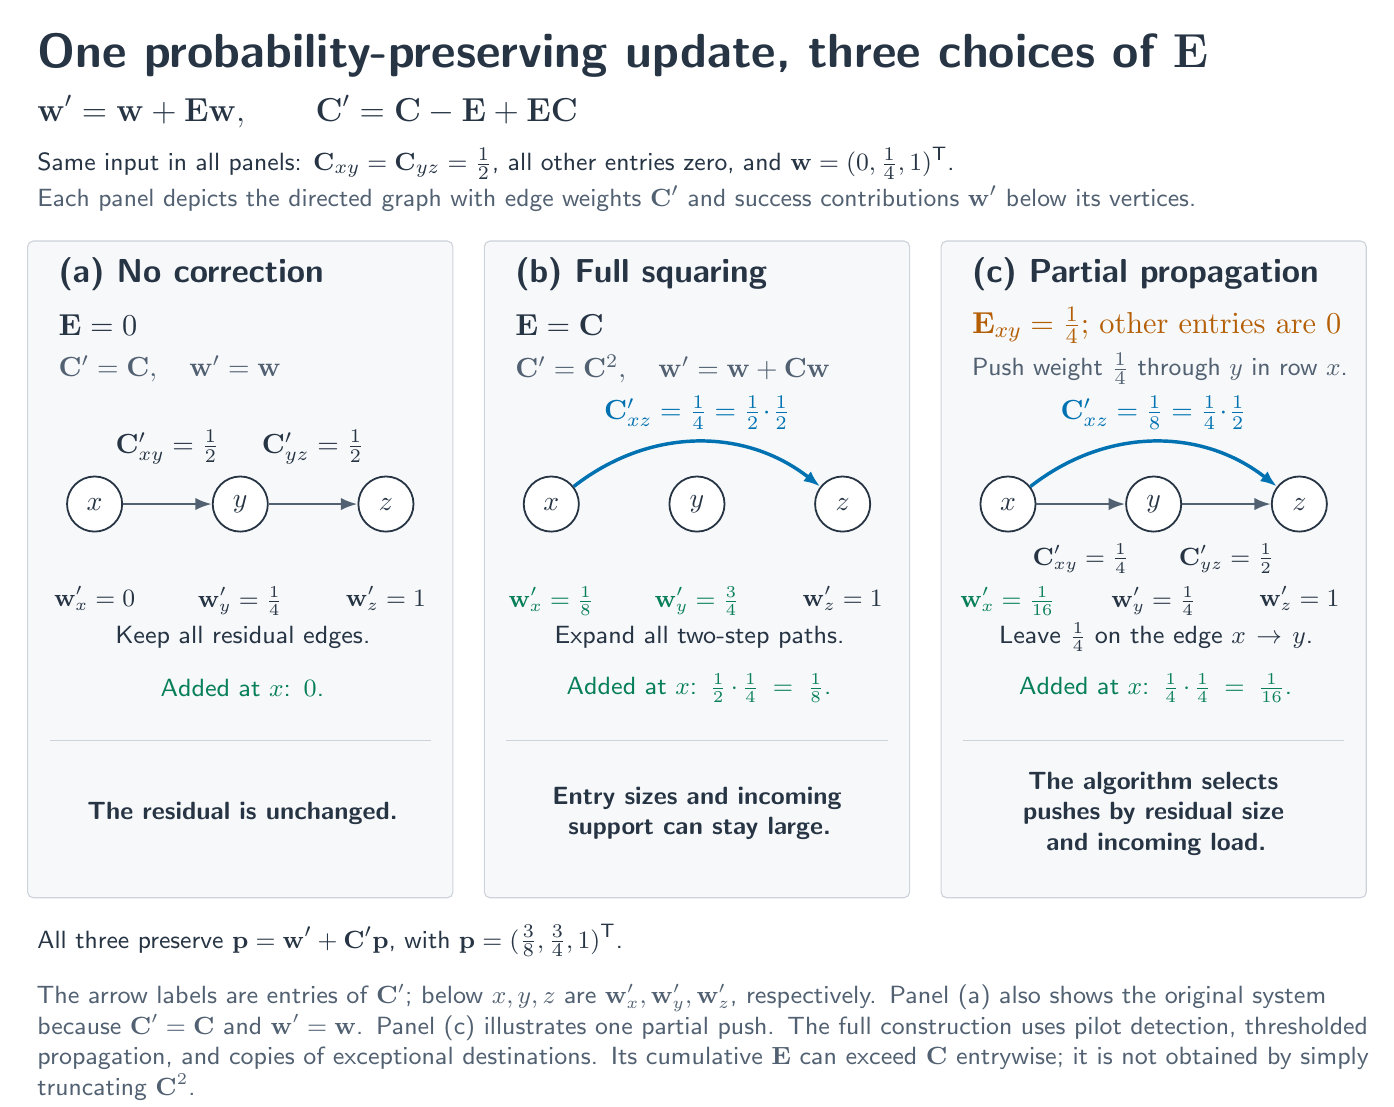
\begin{tikzpicture}[
  x=1cm,y=1cm,text=ink,
  font=\sffamily\fontsize{10}{12}\selectfont,
  vertex/.style={circle,draw=ink,line width=.65pt,fill=white,
    minimum size=7mm,inner sep=0pt,font=\normalsize},
  oldedge/.style={-{Latex[length=2.1mm]},draw=muted,line width=.95pt},
  newedge/.style={-{Latex[length=2.1mm]},draw=shortcut,line width=1.25pt},
  elabel/.style={fill=panelgray,inner sep=2pt,font=\normalsize},
  body/.style={align=center,text width=4.55cm,font=\sffamily\fontsize{9}{11}\selectfont}
]
\path[use as bounding box] (0,-2.25) rectangle (17.0,11.10);

\node[anchor=west,font=\sffamily\bfseries\fontsize{16}{19}\selectfont]
  at (0,10.75) {One probability-preserving update, three choices of $\mE$};
\node[anchor=west,font=\fontsize{12}{15}\selectfont] at (0,10.03)
  {$\displaystyle \vw'=\vw+\mE\vw,\qquad \mC'=\mC-\mE+\mE\mC$};
\node[anchor=west,font=\sffamily\fontsize{9.5}{12}\selectfont] at (0,9.38)
  {Same input in all panels: $\mC_{xy}=\mC_{yz}=\tfrac12$, all other entries zero, and $\vw=(0,\tfrac14,1)^{\mathsf T}$.};
\node[anchor=west,text=muted,font=\sffamily\fontsize{9.5}{12}\selectfont] at (0,8.93)
  {Each panel depicts the directed graph with edge weights $\mC'$ and success contributions $\vw'$ below its vertices.};

% Panel (a): the original system is unchanged.
\begin{scope}[shift={(0,0)}]
  \filldraw[fill=panelgray,draw=linegray,rounded corners=2pt] (0,.05) rectangle (5.4,8.39);
  \node[anchor=west,font=\sffamily\bfseries\fontsize{11.5}{14}\selectfont] at (.27,7.97) {(a) No correction};
  \node[anchor=west,font=\fontsize{11}{13}\selectfont] at (.27,7.32) {$\mE=0$};
  \node[anchor=west,text=muted,font=\fontsize{10}{12}\selectfont] at (.27,6.77) {$\mC'=\mC,\quad\vw'=\vw$};
  \node[vertex] (ax) at (.85,5.05) {$x$};
  \node[vertex] (ay) at (2.70,5.05) {$y$};
  \node[vertex] (az) at (4.55,5.05) {$z$};
  \draw[oldedge] (ax) -- node[elabel,above=12pt] {$\mC'_{xy}=\tfrac12$} (ay);
  \draw[oldedge] (ay) -- node[elabel,above=12pt] {$\mC'_{yz}=\tfrac12$} (az);
  \node[below=16pt of ax,font=\fontsize{9}{11}\selectfont] {$\vw'_x=0$};
  \node[below=16pt of ay,font=\fontsize{9}{11}\selectfont] {$\vw'_y=\tfrac14$};
  \node[below=16pt of az,font=\fontsize{9}{11}\selectfont] {$\vw'_z=1$};
  \node[body] at (2.7,3.36) {Keep all residual edges.};
  \node[body,text=gain] at (2.7,2.71) {Added at $x$: $0$.};
  \draw[linegray] (.28,2.05)--(5.12,2.05);
  \node[body,font=\sffamily\bfseries\fontsize{9}{11}\selectfont] at (2.7,1.12)
    {The residual is unchanged.};
\end{scope}

% Panel (b): E=C produces C squared, including the reward update at y.
\begin{scope}[shift={(5.8,0)}]
  \filldraw[fill=panelgray,draw=linegray,rounded corners=2pt] (0,.05) rectangle (5.4,8.39);
  \node[anchor=west,font=\sffamily\bfseries\fontsize{11.5}{14}\selectfont] at (.27,7.97) {(b) Full squaring};
  \node[anchor=west,font=\fontsize{11}{13}\selectfont] at (.27,7.32) {$\mE=\mC$};
  \node[anchor=west,text=muted,font=\fontsize{10}{12}\selectfont] at (.27,6.77) {$\mC'=\mC^2,\quad\vw'=\vw+\mC\vw$};
  \node[vertex] (bx) at (.85,5.05) {$x$};
  \node[vertex] (by) at (2.70,5.05) {$y$};
  \node[vertex] (bz) at (4.55,5.05) {$z$};
  \draw[newedge] (bx) to[out=38,in=142] node[elabel,above=2pt,text=shortcut] {$\mC'_{xz}=\tfrac14=\tfrac12\!\cdot\!\tfrac12$} (bz);
  \node[below=16pt of bx,text=gain,font=\fontsize{9}{11}\selectfont] {$\vw'_x=\tfrac18$};
  \node[below=16pt of by,text=gain,font=\fontsize{9}{11}\selectfont] {$\vw'_y=\tfrac34$};
  \node[below=16pt of bz,font=\fontsize{9}{11}\selectfont] {$\vw'_z=1$};
  \node[body] at (2.7,3.36) {Expand all two-step paths.};
  \node[body,text=gain] at (2.7,2.71) {Added at $x$: $\tfrac12\!\cdot\!\tfrac14=\tfrac18$.};
  \draw[linegray] (.28,2.05)--(5.12,2.05);
  \node[body,font=\sffamily\bfseries\fontsize{9}{11}\selectfont] at (2.7,1.12)
    {Entry sizes and incoming \mbox{support} can stay large.};
\end{scope}

% Panel (c): one illustrative push, not the entire threshold/pilot algorithm.
\begin{scope}[shift={(11.6,0)}]
  \filldraw[fill=panelgray,draw=linegray,rounded corners=2pt] (0,.05) rectangle (5.4,8.39);
  \node[anchor=west,font=\sffamily\bfseries\fontsize{11.5}{14}\selectfont] at (.27,7.97) {(c) Partial propagation};
  \node[anchor=west,text=choice,font=\fontsize{11}{13}\selectfont] at (.27,7.32) {$\mE_{xy}=\tfrac14$; other entries are $0$};
  \node[anchor=west,text=muted,font=\sffamily\fontsize{9.5}{12}\selectfont] at (.27,6.77) {Push weight $\tfrac14$ through $y$ in row $x$.};
  \node[vertex] (cx) at (.85,5.05) {$x$};
  \node[vertex] (cy) at (2.70,5.05) {$y$};
  \node[vertex] (cz) at (4.55,5.05) {$z$};
  \draw[oldedge] (cx) -- node[elabel,below=12pt,font=\fontsize{9}{11}\selectfont] {$\mC'_{xy}=\tfrac14$} (cy);
  \draw[oldedge] (cy) -- node[elabel,below=12pt,font=\fontsize{9}{11}\selectfont] {$\mC'_{yz}=\tfrac12$} (cz);
  \draw[newedge] (cx) to[out=38,in=142] node[elabel,above=2pt,text=shortcut] {$\mC'_{xz}=\tfrac18=\tfrac14\!\cdot\!\tfrac12$} (cz);
  \node[below=16pt of cx,text=gain,font=\fontsize{9}{11}\selectfont] {$\vw'_x=\tfrac1{16}$};
  \node[below=16pt of cy,font=\fontsize{9}{11}\selectfont] {$\vw'_y=\tfrac14$};
  \node[below=16pt of cz,font=\fontsize{9}{11}\selectfont] {$\vw'_z=1$};
  \node[body] at (2.7,3.36) {Leave $\tfrac14$ on the edge $x\to y$.};
  \node[body,text=gain] at (2.7,2.71) {Added at $x$: $\tfrac14\!\cdot\!\tfrac14=\tfrac1{16}$.};
  \draw[linegray] (.28,2.05)--(5.12,2.05);
  \node[body,font=\sffamily\bfseries\fontsize{9}{11}\selectfont] at (2.7,1.12)
    {The algorithm selects pushes by residual size and incoming load.};
\end{scope}

\node[anchor=west,font=\sffamily\fontsize{9.5}{12}\selectfont] at (0,-.49)
  {All three preserve $\vp=\vw'+\mC'\vp$, with $\vp=(\tfrac38,\tfrac34,1)^{\mathsf T}$.};
\node[anchor=north west,align=left,text width=16.9cm,text=muted,
  font=\sffamily\fontsize{9}{11}\selectfont] at (0,-.92)
  {The arrow labels are entries of $\mC'$; below $x,y,z$ are $\vw'_x,\vw'_y,\vw'_z$, respectively. Panel (a) also shows the original system because $\mC'=\mC$ and $\vw'=\vw$. Panel (c) illustrates one partial push. The full construction uses pilot detection, thresholded propagation, and copies of exceptional destinations. Its cumulative $\mE$ can exceed $\mC$ entrywise; it is not obtained by simply truncating $\mC^2$.};
\end{tikzpicture}

}
\caption{The two extreme choices and one partial propagation. Edge labels give residual transition weights; node values give accumulated success contributions. The full construction adds pilot selection, thresholds, and copying.}
\label{fig:three-choices}
\end{figure}

For the linear-system interpretation, put \(\mathbf A=\mathbf I-\mathbf C\). Then
\[
 \mathbf I-\mathbf C'=(\mathbf I+\mathbf E)\mathbf A,\qquad
 \mathbf w'=(\mathbf I+\mathbf E)\mathbf w.
\]
The step left-preconditions the system by \(\mathbf I+\mathbf E\), preserving its solution. A Richardson step for this preconditioned system, starting at zero, returns \(\mathbf w'\), with error \(\mathbf C'\mathbf p\). The outer construction repeatedly improves the representation of the system; it is not simply Richardson iteration with one fixed preconditioner.

\subsection{Choosing the correction: where to propagate, how much, and what to copy}

At one stage, let \(f\) bound the entries of \(\mathbf C\). A row has at most \(1/(\delta f)\) entries of size at least \(\delta f\), because its total weight is at most one. A column has no such automatic bound: many different rows can send substantial weight to the same destination.

For a raw propagation matrix \(\mathbf G\), the relevant \emph{incoming load} at \(y\) is the count
\[
 \#\{x:\mathbf G_{xy}\geq\delta f\},
\]
at the fixed support threshold \(\delta\) under discussion. A column is crowded when this exceeds a fixed constant times \(1/f\). This is a scale-dependent count of substantial predecessors, not the column sum or a per-vertex memory allocation.

Why control this count? Later we retain each source with probability comparable to \(f\). A bound of order \(1/f\) gives a constant expected number of retained predecessors. A further gate imposes a hard constant bound on the actual correction table in every environment. This supports forward and backward movement through a sampled correction and bounds how many old sources can charge an error at one midpoint. Both uses matter. Low incoming load alone does not prove that the whole recursive state fits in logarithmic space.

Suppose a fixed multiplier vector \(\mathbf g\), with entries in \([0,1]\), says where propagation is allowed. One enables it fully; zero disables it. Beginning with \(\mathbf E_0=0\), perform a constant number of sweeps:
\begin{equation}
 \mathbf G'_i=\mathbf C+\mathbf E_{i-1}\mathbf C,\qquad
 \mathbf E_{i,xy}
   =f\,\mathsf Q(\mathbf G'_{i,xy}/f)\mathbf g_y.
 \label{eq:overview-sweeps}
\end{equation}
The function \(\mathsf Q\) smoothly removes the excess above a small threshold:
\[
 (t-\theta_2)_+\leq\mathsf Q(t)\leq(t-\theta_1)_+,
 \qquad 0<\theta_1<\theta_2.
\]
The raw matrix includes newly propagated weight. The assignment to \(\mathbf E_i\) replaces the cumulative correction; it does not add that correction again to \(\mathbf E_{i-1}\).

The positive remainder serves more than nonnegativity. At a fixed point, every corrected position retains at least \(\theta_1 f\), so a row can correct only \(O(1/f)\) positions. Paths move forward through this bounded set. Counting those ordered paths bounds the tail after \(k\) sweeps by a constant multiple of \(c^k/k!\). A sufficiently large \emph{constant} number of sweeps therefore suffices, independently of the graph size. The remainder also makes subtraction stable: the residual dominates a fixed multiple of the sum of the unsigned terms in \(\mathbf C-\mathbf E+\mathbf E\mathbf C\).

We still need \(\mathbf g\). Testing the incoming load of \(\mathbf C\) once would miss crowding created by propagation. The construction uses a pilot calculation to detect crowding as it develops, freezes its decisions, and restarts the actual correction.

\begin{algorithm}[label=alg:overview-stage]{One exact outer stage}
\textbf{Input.} A forward substochastic matrix \(\mathbf C\) with entries at most \(f\), and accumulated success vector \(\mathbf w\). This describes exact targets; the expectations are not assumed available as small-space subroutines.
\begin{enumerate}[leftmargin=*]
\item \textbf{Pilot.} From zero pilot correction, form \(\mathbf G_i=\mathbf C+\widehat{\mathbf E}_{i-1}\mathbf C\). Sample sources and destinations at rate comparable to \(f\), suppressing sampled rows with too many substantial entries. At each column, take the conditional expected score for having many substantial retained predecessors, conditioned on retaining that column.
\item \textbf{Freeze.} A smooth decreasing function of the largest score seen so far gives a multiplier for each column. After the fixed number of pilot sweeps, freeze these multipliers as \(\mathbf g\).
\item \textbf{Restart and propagate.} Set the actual correction to zero and run \eqref{eq:overview-sweeps} with this fixed \(\mathbf g\). Let \(\mathbf E\) be the last correction.
\item \textbf{Update.} Form \(\mathbf D=\mathbf C-\mathbf E+\mathbf E\mathbf C\) and \(\widetilde{\mathbf w}=\mathbf w+\mathbf E\mathbf w\).
\item \textbf{Copy.} Divide remaining large entries among a fixed number of destination copies using prescribed routing fractions and row factors. Transport \(\widetilde{\mathbf w}\) by the same weighted projection. The next entry bound is \(f/2^h\).
\end{enumerate}
\textbf{Output.} The next exact residual matrix and accumulated success vector.
\end{algorithm}

Pilot scores are deterministic expectations: later noisy estimates do not redefine these targets. The score is an order statistic that becomes large when sufficiently many sampled predecessors contribute. The row gate lets the scores themselves have bounded-access representations. The running maximum remembers crowding in earlier sweeps. Freezing before restarting gives a monotone actual recurrence to which the fixed-point analysis applies.

Fully enabled columns acquire small residual entries. Large remaining entries occur only at exceptional columns. Each exceptional column accounts for many substantial pilot incidences; row-sum bounds limit the total number of incidences. There are therefore few exceptional columns, and their extra copies increase the active-vertex count by at most a factor of two.

Copying changes the domain. A weighted projection \(\mathbf P\) from new vertices to old ones satisfies
\[
 \mathbf C^+\mathbf P=\mathbf P\mathbf D,\qquad
 \mathbf w^+=\mathbf P\widetilde{\mathbf w}.
\]
The new solution vector is \(\mathbf P\mathbf p\). A primary copy has projection weight one and preserves its parent's value. Following primary copies preserves the original start value. This qualifies the simpler fixed-domain picture \eqref{eq:overview-invariant}.

\subsection{Sparse tables: sampling, support bounds, and bias correction}

We do not build the large matrices and conditional expectations of the exact construction. We represent their contributions as conditional means of random tables that can be queried locally.

Entries of size about \(a\) occur only \(O(1/a)\) times in a row of bounded total weight. Retaining destinations with probability comparable to \(a\) leaves a constant expected number. This explains the division into magnitude scales: one sampling rate would oversample some rows or miss their fine contributions.

An expected bound is insufficient for an algorithm that must fit in space on every seed. A row gate suppresses a table row whenever too many retained entries are substantial; correction tables also have an incoming gate. These gates introduce bias. A preparatory conditional mean corrects it. For a fixed scalar contribution \(k_{xy}\), a random gate \(R\), and the relevant retention event \(\mathcal C_{xy}\), the basic calculation is
\[
 q_{xy}=\mathbb E[R\mid\mathcal C_{xy}],\qquad
 B_{xy}=k_{xy}R/q_{xy},\qquad
 \mathbb E[B_{xy}\mid\mathcal C_{xy}]=k_{xy}.
\]
The construction bounds \(q_{xy}\) away from zero wherever the contribution is needed. The actual formula includes support cutoffs and a clipped denominator, with the preparatory task defined before the normalized task. Exact identities apply to true inputs; estimated inputs introduce errors that require analysis.

The connection with Bencz\'ur--Karger sampling~\cite{BenczurKarger2015} is sampling followed by compensating weights. Their cut sparsifier preserves all cuts of an undirected graph simultaneously. Here a sparse table has the required conditional mean, bounded access, and controlled error after averaging. A single environment need not approximate the whole residual matrix well, preserve all cuts, or preserve all quadratic forms. Later row compression is a different operation: it represents a raw row by a default and exceptions.

Polynomial evaluation supplies a short sampling description: keep a bounded number of coefficients and test membership at the queried identifier. We require comparable marginals, a conditional pair bound, a lower-tail count bound, and invariance under the common affine change induced by appending copy symbols. Full independence of all retained vertices is unnecessary.

\subsection{What expansion does, and why an arbitrary expander is insufficient}

The expander operates on \emph{sampling environments}, not on the configuration graph. For an entry \((x,y)\), the environment is conditioned to retain \(x\) on one channel and \(y\) on another. Averaging must preserve these events and approach the corresponding conditional mean uniformly over identifiers and rates.

The interface has two parts. Analytically, each conditional slice has a stationary averaging operator with a uniform spectral gap, giving exponentially decreasing \(L_8\) error with walk length. Computationally, the walk has a short description that survives recursive calls without retaining all the identifiers on which it is conditioned. The construction provides boundedly many invertible variants whose validity is tested when an identifier becomes available. Exactly one variant represents each genuine conditional step.

A sampling channel uses a polynomial coefficient matrix \(\mathbf A=(\mathbf a_0,\mathbf F)\) over \(\mathbb F_{p_{\rm fld}}\), conditioned on the nonconstant columns \(\mathbf F\) being linearly independent. Conditional on retaining an identifier \(y\), the environment can be parametrized by an independent uniform frame \(\mathbf F\) and a uniform vector \(\mathbf z\) in a box of side \(l_{\rm box}\). These choices and \(y\) determine the constant coefficient.

The infinite group is
\[
 \mathcal G_h=\mathrm{SL}_h(\mathbb Z)\ltimes\mathbb Z^h,\qquad h\geq3.
\]
It acts by
\[
 (\mathbf F,\mathbf z)\longmapsto
 (\mathbf M\mathbf F\bmod p_{\rm fld},
       \mathbf M\mathbf z+\mathbf c\bmod l_{\rm box}).
\]
The moduli need not agree. The linear part moves any frame to any other, and translations move the box coordinate, so the finite action is transitive. Its image is a finite quotient of \(\mathcal G_h\): the action is a homomorphism into a finite permutation group, whose kernel can be quotiented out. The state space itself is a homogeneous space, and the averaging graph is a Schreier graph; it need not be a Cayley graph of the whole quotient.

Property~(T) of \(\mathrm{SL}_h(\mathbb Z)\), together with relative property~(T) for the two-dimensional affine group, supplies a uniform gap. Section~\ref{sec:averaging} derives it from Shalom's quantitative results. This is not merely expansion of \(\mathrm{SL}_2(\mathbb F_p)\).

A replacement based on zig-zag expanders~\cite{ReingoldVadhanWigderson2002} would be useful if it supplied both conditional mixing and the implementation properties above, along with sampling identities and copy invariance. A strongly explicit graph with a spectral gap alone does not provide this interface. Transitivity alone does not specify how retention events, actions, and short validated descriptions fit together. This list explains the concrete construction's role; we do not assert a general substitution theorem for arbitrary expanders or transitive codes.

\subsection{What an accuracy level asks the estimator to do}

There is no probability budget assigned to a vertex. The integer \(m\) is an \emph{accuracy level of a query}. With the task's stage, scale, start-retention rate, and dependency rank, it defines an estimator and its access relation. A larger level changes the calculation, not the true target.

The level has three operational effects. Small levels make a task inactive: return zero and empty access. Active tasks call earlier tasks at smaller levels. The parent--child decrease determines how much conditional averaging to perform and how much information a suspended call can retain.

The assigned effective accuracy exponent is
\begin{equation}
 p_{\rm acc}=\frac{m}{k_{\rm prec}}
       -\frac12\log_2\frac1a-\frac12\log_2\frac1u-a_*i_*.
 \label{eq:overview-accuracy}
\end{equation}
Here \(a\) is entry scale, \(u\) is start-retention rate, and \(i_*\) is dependency rank. These deductions pay for scale changes, changes of conditioning, and propagation through earlier tasks. A nonpositive exponent triggers the zero answer. Otherwise the intended error is a fixed constant times \(2^{-p_{\rm acc}}\) in specified moment norms. Thus \(m\) is not itself a number of correct output bits.

Let \(T_r\) denote one scalar sample expression after replacing all earlier inputs by child-level-\(r\) estimates. The level-zero term is zero; exact base contributions are inserted separately. Write successive improvements as
\[
 T_{r_{\max}}=\sum_{r=1}^{r_{\max}}(T_r-T_{r-1}).
\]
The algorithm averages \(T_r-T_{r-1}\) using a conditional walk of length proportional to \(m-r\), with scale-dependent cutoffs on \(r\). Both terms use the \emph{same} walk. Early terms can be large but receive longer averaging. Later differences are smaller because both estimates are already accurate. Mean error and remaining averaging noise are bounded separately.

This relates to varying-accuracy evaluation of stochastic-matrix products~\cite{CohenDoronSberloTaShma2023}. Here the schedule must also pay for conditioning, sparse access, and suspended recursion. If \(d\leq m-r<2d\), a candidate contribution has an \(O(d)\)-bit description and calls a child of level at most \(m-d\). These decreases telescope along a chain to \(O(m)\), allowing the accuracy level to serve both error analysis and space accounting.

\begin{algorithm}[label=alg:overview-query]{Estimate one entry at accuracy level \(m\)}
\textbf{Input.} A task specifying its exact target and common parameters, a queried entry, and one shared sampling environment.
\begin{enumerate}[leftmargin=*]
\item If the effective accuracy exponent is nonpositive, return zero with empty access.
\item Express the raw signal as direct, product, projection, or vector sample terms. Average consecutive-level differences at each included scale.
\item Process contributions in groups of comparable level decrease. Combine contributions at the same destination, then compress the row to a default and a controlled number of exceptions. Small-decrease groups use short fingerprints; adaptive collisions are included in the analysis.
\item Apply row functions, preparatory normalization, incoming gates, and frozen multipliers in dependency order. Return a requested value or access information by recomputation.
\end{enumerate}
\textbf{Convention.} A numerical digit request evaluates this fixed estimator more precisely; it does not redefine the task or its access graph.
\end{algorithm}

\subsection{From local queries to a deterministic answer}

The approximate values must be accurate often enough; their implicit tables must always have bounded access; and their evaluation must always fit in space and terminate. These are separate obligations.

Compression controls row descriptions, but later destinations can depend on earlier fingerprint collisions. A fixed-pair hashing bound is insufficient. The proof compares the actual computation with one using exact equality throughout a block of accuracy levels. This yields a candidate set independent of that block's hash seed; departures from the set are charged to lower-level errors. Estimator accuracy and comparison error are proved together.

For space, bounding one local call by \(O(\log n)\) would still permit an \(O(\log^2 n)\) stack. The implementation shares long-lived workspace and regenerates local data. Each suspended record is charged to a decrease in call allowance and, for arithmetic, a change in requested digit place. These charges telescope. The proof counts shared workspace, all suspended records, traversal data, and arithmetic scratch. It proves termination even on seeds giving poor estimates.

The environment has \(O(\log n)\) bits. After paying for the conversion from average error to the specified start, the moment bound shows that a fixed majority of appropriate environments give accurate answers. Enumerate them deterministically and take a median by repeated counting passes. Recompute estimates as needed instead of storing their list. Preserve the multiplicity of original seed encodings so enumeration matches the analyzed probability law.

Choose hierarchy depth, query level, and output digit precision so their three errors sum to the requested tolerance. For bounded-error decision, compare the answer with \(1/2\); for arbitrary acceptance probabilities, return the approximation.

\subsection{Undirected connectivity and Laplacian solvers}

Undirected connectivity is a special case. A sufficiently long polynomial-time random walk finds a reachable target with constant probability by the usual hitting bound~\cite{AleliunasKLLR1979}. Apply this algorithm to the time-layered walk and threshold its acceptance probability. Even for an undirected input, the construction works with a directed forward configuration graph and residual continuation values.

Reingold's algorithm~\cite{Reingold2008} instead improves expansion within connected components, using powering and degree reduction, then enumerates short walks. The zig-zag product of Reingold, Vadhan, and Wigderson~\cite{ReingoldVadhanWigderson2002} controls degree while retaining expansion; Rozenman--Vadhan derandomized squaring~\cite{RozenmanVadhan2005} is another related route. Here partial propagation resolves a linear system, while the auxiliary expander mixes conditional sampling environments. These are distinct uses of expansion.

The connection with Spielman--Teng~\cite{SpielmanTeng2014} is preconditioning and recursive approximate computation. Their nearly-linear-time solver uses symmetric diagonally dominant structure and energy-norm approximation. Here the directed, time-layered system \(\mathbf I-\mathbf C\) is analyzed using nonnegativity, forward order, conditional moments, and total live memory. Its sparse tables are not spectral preconditioners. A closer space-complexity precedent is the Laplacian solver of Murtagh, Reingold, Sidford, and Vadhan~\cite{MurtaghReingoldSidfordVadhan2017}, which combines fast-solver ideas with small-space graph operations.

The formal proof now defines the model and sampling interface, constructs the exact reduction, builds and averages sparse tables, analyzes recursive accuracy and compression, realizes the queries within bounded total memory, and takes the final median.




% ---- sections/model ----
% Pedagogical rewrite, October 8, 2026. Original mathematics: OpenAI.
\section{The transition model and resource parameters}\label{sec:model}

We now make the configuration-graph description precise. Two choices in this reduction will be used throughout the proof. Time is part of the vertex, so the transition matrix has no directed cycles. Also, a vertex retains the complete configuration, even after the machine halts. This gives a bounded list of predecessors as well as successors. Merging all accepting configurations into one sink would lose the predecessor bound.

The reduction gives continuation probabilities at every vertex, not only at the designated start. This stronger conclusion is needed because the later construction takes weighted copies of these probabilities.

We use machines with finite control, an endmarked read-only input,
finitely many work tapes, and fresh independent fair bits. Input heads
are confined between the endmarkers. All randomized running-time
bounds hold on every random tape. Space counts traversed writable cells
in bits, including every simultaneously live counter, numerical register
and suspended call; visiting a blank work cell counts toward space.
A transducer has a one-way write-only output tape. Throughout,
$n$ is the input length and logarithms have base two.


A matrix indexed by a finite set $V$ is \emph{strictly forward} if
there is an integer time attached to every vertex and every nonzero
entry goes to a strictly later time. It is \emph{substochastic} if its
entries are nonnegative and each row sums to at most one. An edge is
specified by a vertex and a port from a fixed finite set. A \emph{paired}
edge operation returns the other endpoint together with its inverse
port; applying the inverse operation restores the first endpoint.
Absent ports are explicitly recognized.

\begin{lemma}[Configuration reduction]\label{lem:model-reduction}
Fix a polynomial-time randomized machine using $O(\log(n+2))$ work
space. On an input of length $n$ one can specify, uniformly in
logarithmic space, a polynomial-size vertex set $V_0$, a strictly
forward substochastic matrix ${\mathbf{S}}$, a vector
${\mathbf{e}}\in\{0,1\}^{V_0}$, and a start vertex $x_0$ with the following
properties.
\begin{enumerate}
\item The incoming and outgoing port degrees of ${\mathbf{S}}$ are bounded by
constants depending only on the machine. Port validity, edge weights,
and pairing are computable in logarithmic space.
\item The vector ${\mathbf{p}}_0=({\mathbf{I}}-{\mathbf{S}})^{-1}{\mathbf{e}}$ is well defined and belongs to
$[0,1]^{V_0}$.
\item The coordinate ${\mathbf{p}}_{0,x_0}$ is the acceptance probability of
the machine.
\end{enumerate}
In particular, an $\RL$ computation gives the promise
${\mathbf{p}}_{0,x_0}=0$ or ${\mathbf{p}}_{0,x_0}\ge1/2$.
\end{lemma}

\begin{proof}
Let ${\mathsf{t}}(n)$ be a fixed polynomial upper bound on the running time.
A vertex records a time in $\{0,\ldots,{\mathsf{t}}(n)\}$, the finite control,
all input and work head positions, and the contents of a sufficiently
large box of $O(\log(n+2))$ work cells. Take elementary machine steps
with fixed dyadic coin probabilities. A transition advances the time
by one. Invalid configurations or moves leaving the box have no
corresponding transition. The box is chosen large enough that this
never affects a computation from the specified start.

We need local access in both directions. Successor access is immediate: each elementary step has constantly many successor choices.
To find predecessors, guess the old finite control, locally overwritten
symbols, head movements, and coin choice, then check that the forward
step gives the specified configuration. There are constantly many such
guesses. Combine transitions with the same ordered pair of endpoints
by adding their probabilities. Order the distinct successors and
predecessors by their configuration encodings; their positions give
paired ports for the resulting matrix entries. These lists have
constant length, so duplicate removal, summed weights, and the inverse
port are computed in logarithmic space by local enumeration. This
base computation makes no recursive graph queries. All records use
$O(\log(n+2))$ bits, and the read-only input can be consulted during
these checks.

The simulated input head is an address stored in a vertex. It must not become an uncounted storage device for the algorithm carrying out the simulation. To ensure this, all input-head coordinates in the vertex universe are restricted to a
fixed polynomial interval containing the positions reachable within
${\mathsf{t}}(n)$ local steps from their specified initial positions. Configurations
and predecessor candidates outside that interval are invalid. To obtain
a simulated head's scanned symbol, compare its stored coordinate with
the input boundaries, supply any required endmarker or off-data blank
according to the source tape convention, and otherwise scan the real
endmarked input to the designated position using a logarithmic-space
counter. A position forbidden by the source tape convention remains
invalid. The physical scan stays between the real endmarkers, even when
a valid simulated coordinate is outside the data. This routine makes
no recursive graph query.

To collect acceptance at one common time, let an already halted computation keep its complete tape and head data while its time advances. These are distinct vertices in successive layers, not self-loops. Keeping the full configuration prevents many unrelated halted computations from merging at one vertex. Let ${\mathbf{e}}$ be one precisely at accepting
configurations at time ${\mathsf{t}}(n)$, and zero elsewhere. Final-time rows
have no outgoing transitions. Thus ${\mathbf{S}}$ is strictly forward and
substochastic, and it is nilpotent. Its inverse expression is the finite
sum
\[
({\mathbf{I}}-{\mathbf{S}})^{-1}{\mathbf{e}}=\sum_{j=0}^{{\mathsf{t}}(n)}{\mathbf{S}}^j{\mathbf{e}}.
\]
Starting from any valid configuration, at most one success contribution can be
collected, at final time. The sum is therefore a probability in
$[0,1]$. At $x_0$ it is exactly the machine's acceptance probability.
\end{proof}

The coordinatewise bound on ${\mathbf{p}}_0$ will be used after weighted projections
to larger vertex sets.  It holds at every configuration, independently
of the acceptance probability at the designated start.  Thus the matrix
construction and the probability approximation below apply to arbitrary
randomized computations satisfying the resource bounds.

\paragraph{The parameters to remember.}
There are three size quantities with different roles. The input has length $n$; a vertex address and the shared randomness will have length $O({b_{\rm mem}})$; and ${n_{\rm v}}$ is an upper bound on the number of vertices at any one stage. The stage index counts copy steps, whereas a sampling-rate index measures how many vertices a random subset is expected to retain. We specify these quantities below before introducing any of the local thresholds.

\paragraph{Size convention.}
Fix an integer parameter ${b_{\rm mem}}$, a power of two, comparable with
$\log_2(n+2)$ and at least a sufficiently large fixed constant.
For example, take the least power of two at least the maximum of that
constant and $\lceil\log_2(n+2)\rceil$.  This choice is computable in
logarithmic space and includes all bounded input lengths in the same
construction. All constants throughout the
construction are independent of the input; they may depend on the fixed
machine and, for fixed inverse-polynomial accuracy, its fixed exponent.
The uniform precision parameter of Theorem~\ref{thm:probability} is
handled separately by padding. The number of stages is ${l_{\rm max}}=O({b_{\rm mem}})$. At stage $l$, a vertex has
a base identifier followed by $l$ symbols from a fixed radix ${d}_0$.
The radix will be selected by the hierarchy. Encode each base vertex by
a fixed-width radix-${d}_0$ word and prepend the digit $1$; unused base
words are invalid. Appending one copy digit at each stage gives
injective numerical identifiers even across different stage lengths.
Indeed, a base width $w$ places stage-$l$ identifiers in
$[{d}_0^{w+l},2{d}_0^{w+l})$, and these intervals are disjoint.
Appending a fixed suffix is an affine map on identifiers.

Every stage has size at most a common bound
\[
{n_{\rm v}}=2^{{c_{\mathrm{bd},n_{\rm v}}}{b_{\rm mem}}}.
\]
We may increase the fixed constant ${c_{\mathrm{bd},n_{\rm v}}}$ as needed. This is a bound on
one stage, not a claim that there are only ${n_{\rm v}}$ pairs of vertices.
Integrated entry errors below carry a factor $1/{n_{\rm v}}$ while summing over both endpoints. This is a normalization per source vertex, not per ordered pair. Later degree bounds control the additional sum over destinations; inserting a second factor of $1/{n_{\rm v}}$ would change the error statement.

Fix integers ${h}\ge4$ and $2\le h_0<{h}$, and put
\[
b_k=2^{-{h}k}\qquad(k\ge0).
\]
These are the nominal sampling rates. Stage $l$ will have density
$f=b_l$. The stochastic tables will use rates from this same grid
for their source and terminal retention tests. The error power in
the later analysis is always $s=8$.

\paragraph{Uniform constants and finite ranges.}
All thresholds needed by the algorithm can be chosen rational, with
fixed gaps, and all discrete constants can be chosen integer. We
first prove estimates with constants uniform in the ambient finite
universe. The sampling construction applies to every finite range of
identifiers and rates once its prime field is sufficiently large.
The hierarchy uses $O({b_{\rm mem}})$ copy digits and rates with $k=O({b_{\rm mem}})$;
Section~\ref{subsec:final-constants} will verify this rate bound also
for the recursive estimator and give a compatible order of constant
choices.

We can then take the prime field to have size $2^{O({b_{\rm mem}})}$, with its
exponent chosen after these constants. Its elements and all identifiers
occupy $O({b_{\rm mem}})$ bits. Increasing that exponent does not change the
probabilistic constants proved in the next section.





% ---- sections/environment ----
% Pedagogical rewrite, October 8, 2026. Original mathematics: OpenAI.
\section{Sampling vertex subsets with a short description}\label{sec:env}

The detector needs to sample rows and columns without writing down a random bit for every vertex. We therefore describe an entire random subset by a small collection of polynomial coefficients. Given the coefficients and one vertex identifier, membership can be tested on demand.

\subsection{The sampling interface}

Before choosing coordinates, specify what the rest of the proof needs. A channel is a short random description of nested subsets of the vertex universe, one subset for each nominal rate. A membership query supplies a vertex and a rate, and returns one bit. The required guarantees are: correct marginal probabilities up to fixed factors, a conditional pair bound after one specified membership is imposed, a lower-tail estimate for the number of hits in a deterministic set, and invariance when a common copy suffix is appended to every identifier. Lemma~\ref{lem:env-ranks} gives their exact quantifiers and constants.

Conditional averaging imposes a further requirement on this same family: it must admit rapidly mixing actions that preserve the required memberships and have short, validated descriptions. Section~\ref{sec:averaging} proves this additional property for the construction below. Separating these requirements explains both why pairwise-independent hashing is a useful starting point and why an arbitrary such hash family is not yet sufficient.

\subsection{Polynomial channels with independent nonconstant columns}

The environment consists of the independent rank channels below together
with a finite string of independent uniform auxiliary bits.  The length
and uses of that string will be specified when needed.

One independently chosen collection of coefficients is called a channel. We use a fixed number of independent rank channels, including channels denoted $X,Y,Z$. Extra channels, when needed, are also a fixed finite
number. A channel is a uniformly random matrix
\[
{\mathbf{A}}=({\mathbf{a}}_0,{\mathbf{F}})\in\mathbb F_{p_{\rm fld}}^{{h}\times h_0}
\]
conditioned on the last $r=h_0-1$ columns ${\mathbf{F}}$ being linearly
independent. We call such an ordered collection of columns a \emph{frame}.
The integer ${p_{\rm fld}}$ is prime. It is chosen larger than every
identifier and sufficiently large for all rate comparisons below.
For a numerical identifier $y$, set
\[
{\mathbf{v}}(y)=(1,y,\ldots,y^{h_0-1})^{\mathsf T},
\qquad {\mathbf{a}}(y)={\mathbf{A}}{\mathbf{v}}(y)\in\mathbb F_{p_{\rm fld}}^{h}.
\]
Field elements in a retention test use their representatives in
$\{0,\ldots,{p_{\rm fld}}-1\}$. At nominal rate $b_k$, let
\[
{l_{\mathrm{box},k}}=\lceil {p_{\rm fld}}2^{-k}\rceil,\qquad
\pi_{b_k}=({l_{\mathrm{box},k}}/{p_{\rm fld}})^{h}.
\]
Evaluate the same polynomial array at each identifier. The identifier is retained if all coordinates of ${\mathbf{a}}(y)$ lie in
$\{0,\ldots,{l_{\mathrm{box},k}}-1\}$. Write $X_a(y)$ for the indicator on channel
$X$ at rate $a$, and similarly for other channels.
The same notation permits a specified fixed suffix in the channel
argument. Retention boxes are nested.
All rates in this section belong to the grid $b_k=2^{-{h}k}$, and the
admissible range satisfies ${p_{\rm fld}}2^{-k}\ge1$. The choices of ${h},h_0$ and
the identifier range are those of Section~\ref{sec:model}.

\begin{lemma}[Rank-channel estimates]\label{lem:env-ranks}
There are positive constants $c_\pi,{c_\pi^+},{c_{\mathrm{bd},\mathrm{pair}}},{c_{\mathrm{bd},\mathrm{var}}}$,
depending only on ${h},h_0$, with the following properties in every
admissible finite range.
\begin{enumerate}
\item A specified identifier is retained at rate $a$ with probability
$\pi_a$, where $c_\pi a\le\pi_a\le {c_\pi^+} a$.
\item For distinct identifiers $x,y$ and any admissible rates $u,a$,
\[
\Pr\{X_a(y)=1\mid X_u(x)=1\}\le {c_{\mathrm{bd},\mathrm{pair}}}a.
\]
\item If ${\mathcal{A}}_0$ is a deterministic set of $q$ distinct identifiers and
$T_a=\sum_{y\in {\mathcal{A}}_0}X_a(y)$, then
\[
\Pr\{T_a<q\pi_a/2\}\le \frac{{c_{\mathrm{bd},\mathrm{var}}}}{q\pi_a}
\quad(q>0).
\]
\item Replacing every channel argument $y$ by the same injective affine
map $\alpha y+\beta$ leaves the joint law of all evaluations unchanged,
provided $\alpha\ne0$ in $\mathbb F_{p_{\rm fld}}$. In particular, a common fixed
padding suffix leaves their law unchanged.
\end{enumerate}
\end{lemma}

\begin{proof}
We first compare the conditioned sampling rule with unrestricted polynomial coefficients. The rank condition has probability bounded below by an absolute positive constant:
\par
The probability that an unrestricted ${h}$-by-$r$ matrix is a frame is
\[
q_{\mathrm{fr}}=\prod_{j=0}^{r-1}(1-{p_{\rm fld}}^{j-{h}})\ge c_{\mathrm{fr}}>0.
\]
For fixed positive-degree coefficients, ${\mathbf{a}}_0$ is uniform, so any one
evaluation is uniform in $\mathbb F_{p_{\rm fld}}^{h}$ and independent of frame
success. This proves the exact marginal retention probability.
In the ranges used, take ${p_{\rm fld}}2^{-k}\ge1$. Then
${p_{\rm fld}}2^{-k}\le {l_{\mathrm{box},k}}\le2{p_{\rm fld}}2^{-k}$, proving comparability. The prime
exponent can in fact make all these sides much larger than one.

For the conditional-pair bound, full independence after rank conditioning is unnecessary. We can first use independence in the unrestricted distribution and then pay for conditioning by the reciprocal of its probability. Without conditioning on a frame, two evaluations at distinct field
points are independent uniform vectors: the two evaluation functionals
have rank two since $h_0\ge2$. Consequently
\[
\Pr\{X_a(y)=1,X_u(x)=1\mid {\mathbf{F}}\text{ is a frame}\}
\le \frac{\pi_a\pi_u}{q_{\mathrm{fr}}}.
\]
The first marginal after conditioning is still $\pi_u$, which proves
the second assertion.

The count estimate uses the same comparison. For the third assertion, in the unrestricted distribution the hit count
has mean $q\pi_a$ and variance at most $q\pi_a$, by pairwise
independence. Chebyshev's inequality bounds the stated lower-tail event
by $4/(q\pi_a)$. Conditioning on frame success increases this probability
by at most $1/q_{\mathrm{fr}}$.

For reuse after copying vertices, substituting $\alpha y+\beta$ in a polynomial acts on its
positive-degree coefficient columns by an invertible triangular
matrix, with diagonal $\alpha,\ldots,\alpha^{h_0-1}$.
It therefore preserves the frame condition. Its action on the full
coefficient array is an invertible linear change of variables, so it
preserves uniform measure conditional on that condition. Appending
digits in radix ${d}_0$ has $\alpha$ a power of ${d}_0$; taking
${p_{\rm fld}}>{d}_0$ ensures the required invertibility.
\end{proof}





% ---- sections/hierarchy ----
% Pedagogical rewrite, October 8, 2026. Original mathematics: OpenAI.
\section{The exact reduction: propagation with controlled incoming support}
\label{sec:hierarchy}

This section constructs the exact target of the estimator. It is useful to keep its final guarantee in view: at each stage, the largest transition entry decreases by a factor $2^{h}$, while the number of vertices incident to positive entries increases by at most a factor of two. The residual transition mass then tends to zero geometrically. Propositions~\ref{prop:hier-copy-step} and~\ref{prop:hier-reward-target} state the one-stage guarantee and its consequence for acceptance probabilities.

There are three operations to justify. A correction transfers transition contributions into the success contribution. A detector restricts that correction in columns with too many substantial incoming entries. A copy step divides the remaining large entries while controlling how many copies become active. We begin with the identity that makes the first operation exact.

Given a transition matrix ${\mathbf{C}}$ and a nonnegative correction ${\mathbf{E}}$, put
\[
 {\mathbf{D}}={\mathbf{C}}-{\mathbf{E}}+{\mathbf{E}}{\mathbf{C}}.
\]
Then ${\mathbf{I}}-{\mathbf{D}}=({\mathbf{I}}+{\mathbf{E}})({\mathbf{I}}-{\mathbf{C}})$. Thus a relation ${\mathbf{w}}=({\mathbf{I}}-{\mathbf{C}}){\mathbf{p}}$ becomes
$({\mathbf{I}}+{\mathbf{E}}){\mathbf{w}}=({\mathbf{I}}-{\mathbf{D}}){\mathbf{p}}$: the same vector ${\mathbf{p}}$ is represented by the new transition
and the updated success contribution. The correction must make ${\mathbf{D}}$ nonnegative and keep
its row sums at most one. It must also reduce entries sufficiently fast
that, after a controlled increase in the number of active vertices, the
remaining transition contribution becomes small.  The construction uses
only the model reduction, with no one-sided acceptance promise.

At one stage the input is a finite ordered set $V$, a rate $0<f\le1$
on the grid of Section~\ref{sec:env}, and a nonnegative matrix ${\mathbf{C}}$ with
\begin{equation}
 {\mathbf{C}}_{xy}=0\quad\text{unless }x<y,\qquad
 {\mathbf{C}}\mathbf1\le\mathbf1,\qquad {\mathbf{C}}_{xy}\le f.
 \label{eq:hier-input}
\end{equation}
All matrix and vector inequalities are entrywise. A scalar cutoff applied to a matrix acts entrywise. Multiplying such an array by a column multiplier means scaling column $y$ by that multiplier at $y$; all transition products, such as $\mathbf E\mathbf C$, are ordinary matrix products. Write
\[
 \mathcal R({\mathbf{C}})=\{x:\text{some }{\mathbf{C}}_{xy}>0\},\quad
 \mathcal T({\mathbf{C}})=\{y:\text{some }{\mathbf{C}}_{xy}>0\},\quad
 \mathcal A({\mathbf{C}})=\mathcal R({\mathbf{C}})\cup\mathcal T({\mathbf{C}}).
\]
The stage will reduce the entry bound from $f$ to $f/2^{h}$ and increase
$|\mathcal A({\mathbf{C}})|$ by at most a factor of two. We first analyze the
correction with an arbitrary fixed column multiplier. We then choose that
multiplier by a finite detector calculation, and use copies to divide the
entries in columns where correction is not fully enabled.

\subsection{Correction with a fixed column multiplier}

The correction will remove most of a sufficiently large entry, but it must leave a small positive remainder. That remainder has two uses. It ensures nonnegativity of the new transition matrix, and its positive size bounds the number of corrected positions in a row. The cutoff ${\mathsf{Q}}$ expresses this rule continuously, so that replacing an input by a nearby estimate has a controlled effect. The gap between its two thresholds leaves room for later errors.

Put $q=2^{h}$.  Fix rational numbers
$0<\theta_1<\theta_2<q^{-1}/32$ and a nondecreasing Lipschitz function
${\mathsf{Q}}:[0,\infty)\to[0,\infty)$ satisfying
\begin{equation}
 (t-\theta_2)_+\leq {\mathsf{Q}}(t)\leq(t-\theta_1)_+.
 \label{eq:hier-Q}
\end{equation}
Its eighth root is required to be Lipschitz on bounded intervals. This extra regularity is used when errors in support decisions are bounded by eighth moments. It is a choice we can build into the cutoff, rather than an additional hypothesis on the input matrix.
Here and below the scalar cutoffs can be chosen piecewise polynomial with
rational coefficients.  To see this explicitly, let $\beta$ be the
normalized integral of $t^7(1-t)^7$ on $[0,1]$, extended by zero to the
left and one to the right.  Both $\beta^{1/8}$ and
$(1-\beta)^{1/8}$ are Lipschitz: near their vanishing endpoints the
corresponding functions vanish to order eight, and away from those
endpoints the assertion follows by differentiation.  For example,
\[
 {\mathsf{Q}}(t)=(t-\theta_1)_+
       \beta\left(\frac{t-\theta_1}{\theta_2-\theta_1}\right)
\]
has all the stated properties.  Near $\theta_1$ its eighth root is of
order $(t-\theta_1)_+^{9/8}$; elsewhere its root has bounded derivative
on every bounded interval.  Let ${l}_{\mathsf{Q}}$ be a fixed Lipschitz constant for
${\mathsf{Q}}$.  For real arguments, extend ${\mathsf{Q}}$ by ${\mathsf{Q}}(t)=0$ when $t<0$.
This extension preserves its Lipschitz and root-Lipschitz properties and
permits evaluation on real approximations.  The exact hierarchy itself
uses only nonnegative arguments.

For the moment, suppose we have already decided how much correction each column permits. Write this decision as a fixed multiplier ${\mathbf{g}}:V\to[0,1]$. A value of one enables the full correction, and a value of zero disables it. Starting from zero, define
\begin{equation}
 {\mathbf{E}}_0=0,\qquad {\mathbf{G}}'_i={\mathbf{C}}+{\mathbf{E}}_{i-1}{\mathbf{C}},\qquad
 {\mathbf{E}}_{i,xy}=f{\mathsf{Q}}({\mathbf{G}}'_{i,xy}/f){\mathbf{g}}_{y}\quad(i\ge1).
 \label{eq:hier-fixed-g-iteration}
\end{equation}
The cutoff leaves a positive residual at each corrected entry.  Keeping
${\mathbf{g}}$ fixed makes the update map monotone.  We next show that a fixed
number of iterations suffices for every such multiplier, independently
of the size of $V$.  At a nonnegative fixed point ${\mathbf{E}}_*$ of this recurrence, put
${\mathbf{T}}={\mathbf{C}}-{\mathbf{E}}_*+{\mathbf{E}}_*{\mathbf{C}}$.  In a column with ${\mathbf{g}}_{y}=1$, the lower bound on ${\mathsf{Q}}$
gives ${\mathbf{T}}_{xy}\le\theta_2f$.  The truncation estimate below will transfer
this entry bound to a finite correction, with a small additional error.
The fixed point is only a comparison object; the hierarchy will use a
finite iteration.

\paragraph{What the fixed-multiplier calculation will establish.}
The remainder left by ${\mathsf{Q}}$ limits how many positions a single row can correct. Forward order then turns iteration error into an ordered-path count, giving a factorial tail rather than a contraction assumption. We postpone that proof until after the pilot and actual constructions are fully specified.

\subsection{Choosing which columns permit correction}

The fixed-multiplier argument did not explain how to choose ${\mathbf{g}}$. We need correction to be enabled only in columns with a controlled number of substantial entries. A preliminary sequence of corrections, called the pilot, estimates how crowded each column is. After that sequence, its final choice of ${\mathbf{g}}$ is frozen and the actual correction starts again from zero. The two sequences serve different purposes: the pilot chooses the multiplier; the actual sequence is the monotone recurrence analyzed above.

At this stage these are exact mathematical definitions. Every detector is a true expectation of an already defined input. Computing an approximation to the detector comes later, so an approximate value never defines its own exact target.

For the detectors we use independent channels $X,Y$ from
Section~\ref{sec:env}.  Denote their common retention probability at rate
$f$ by $\pi_f$.  The consequences of Lemma~\ref{lem:env-ranks} needed here
can be written, with fixed positive constants, as
\begin{align}
 c_\pi f\leq\pi_f\leq {c_\pi^+} f,\qquad
 &\Pr\{Y_f(w)=1\mid Y_f(y)=1\}\leq {c}_{\mathrm{pair}} f
       &&(w\ne y), \label{eq:hier-sampling-pair}\\
 &\Pr\left\{\sum_{x\in {\mathcal{A}}}X_f(x)<\tfrac12|{\mathcal{A}}|\pi_f\right\}
       \leq\frac{{c}_{\mathrm{var}}}{|{\mathcal{A}}|\pi_f}
       &&(\varnothing\ne {\mathcal{A}}\subseteq V\text{ deterministic}).
       \label{eq:hier-sampling-tail}
\end{align}
These constants are uniform in the stage, the admissible moduli, and common
fixed padding suffixes.  No independence between different rows of a
detector trial will be assumed.

All threshold choices and ranks below are fixed constants.  The pilot
uses the iteration count from Lemma~\ref{lem:hier-fixed-point}.  Choose
\[
 0<\delta_0<\delta_1<\theta_1/100,
 \qquad 0<\eta_-<\eta_+<\delta_0/3.
\]
If other row scores require still smaller detector thresholds, make those
choices before fixing the ranks.  Let $\phi$ be a nondecreasing cutoff
which is zero through $\delta_0$ and one from $\delta_1$ on.  Let $\rho$
be a nonincreasing cutoff which is one through $\eta_-$ and zero from
$\eta_+$ on.  Finally, let $\gamma:[0,1]\to[0,1]$ be nonincreasing,
one on $[0,1/2]$, and zero on $[4/5,1]$.  These functions and their
complements, when used, have the root regularity just described.

A detector looks for many retained rows that contribute substantially to the same column. It must first exclude rows with too many sampled entries, because those rows will not support a bounded-access representation. The row gate ${\mathbf{r}}^{\rm gate}_i$ performs this exclusion; the ${j_{\rm det}}$th-largest score then tests whether enough eligible rows remain.

For a finite multiset of nonnegative numbers, $\operatorname{rank}_j$
means its $j$-th largest member, with enough additional zeros that this is
always defined.  Starting from $\widehat {\mathbf{E}}_0=0$, perform $k_*$ pilot
steps.  At step $i$, first set
\begin{equation}
 {\mathbf{G}}_i={\mathbf{C}}+\widehat {\mathbf{E}}_{i-1}{\mathbf{C}}.
 \label{eq:hier-pilot-input}
\end{equation}
For a draw of the terminal channel, set
\begin{equation}
 {\mathbf{r}}^{\rm gate}_{i,x}=\rho\left(\operatorname{rank}_{k_{\rm row}}
       \{{\mathbf{G}}_{i,xw}/f:Y_f(w)=1\}\right).
 \label{eq:hier-pilot-row-gate}
\end{equation}
Define the deterministic column number
\begin{equation}
 {\mathbf{u}}_{i,y}=\mathbb E\left[
    \operatorname{rank}_{j_{\rm det}}
       \{\phi({\mathbf{G}}_{i,xy}/f){\mathbf{r}}^{\rm gate}_{i,x}:X_f(x)=1\}
       \,\middle|\,Y_f(y)=1\right].
 \label{eq:hier-detector}
\end{equation}
Then put
\begin{equation}
 \widehat {\mathbf{g}}_{i,y}=\gamma\left(\max_{1\leq r\leq i}{\mathbf{u}}_{r,y}\right),
 \qquad
 \widehat {\mathbf{E}}_{i,xy}=f{\mathsf{Q}}({\mathbf{G}}_{i,xy}/f)\widehat {\mathbf{g}}_{i,y}.
 \label{eq:hier-pilot-correction}
\end{equation}
The order of these definitions is essential: ${\mathbf{G}}_i$ is already
deterministic when its detector is formed, and ${\mathbf{u}}_i$ is defined before
$\widehat {\mathbf{E}}_i$.  The running maximum makes $\widehat {\mathbf{g}}_i$ nonincreasing.
Its final value is therefore no larger than any earlier pilot multiplier;
monotonicity of ${\mathsf{Q}}$ will let us bound the actual corrections by the pilot
corrections.

After the pilot, set ${\mathbf{g}}=\widehat {\mathbf{g}}_{k_*}$ and specialize the fixed-multiplier
recurrence of Equation~\eqref{eq:hier-fixed-g-iteration} to the actual correction
\begin{equation}
 {\mathbf{E}}_0=0,\qquad {\mathbf{G}}'_i={\mathbf{C}}+{\mathbf{E}}_{i-1}{\mathbf{C}},\qquad
 {\mathbf{E}}_{i,xy}=f{\mathsf{Q}}({\mathbf{G}}'_{i,xy}/f){\mathbf{g}}_{y}\quad(1\leq i\leq k_*).
 \label{eq:hier-actual-iteration}
\end{equation}
Write
\begin{equation}
 {\mathbf{E}}={\mathbf{E}}_{k_*},\qquad {\mathbf{D}}={\mathbf{C}}-{\mathbf{E}}+{\mathbf{E}}{\mathbf{C}}.
 \label{eq:hier-residual-definition}
\end{equation}

\begin{algorithm}[label=alg:exact-stage]{Pilot, frozen correction, and copying}
\textbf{Input.} The stage data in \eqref{eq:hier-input}, its success vector ${\mathbf{w}}$, and the fixed cutoffs and ranks specified here.
\begin{enumerate}[leftmargin=*]
\item Set $\widehat {\mathbf{E}}_0=0$. For $i=1,\ldots,k_*$, compute ${\mathbf{G}}_i$, the row gate ${\mathbf{r}}^{\rm gate}_i$, and the exact detector vector ${\mathbf{u}}_i$ by \eqref{eq:hier-pilot-input}--\eqref{eq:hier-detector}. Update $\widehat {\mathbf{g}}_i,\widehat {\mathbf{E}}_i$ by \eqref{eq:hier-pilot-correction}.
\item Freeze ${\mathbf{g}}=\widehat {\mathbf{g}}_{k_*}$. Restart ${\mathbf{E}}_0=0$, then perform the $k_*$ updates in \eqref{eq:hier-actual-iteration}. Set ${\mathbf{E}}={\mathbf{E}}_{k_*}$.
\item Form ${\mathbf{D}}={\mathbf{C}}-{\mathbf{E}}+{\mathbf{E}}{\mathbf{C}}$ and $\widetilde {\mathbf{w}}={\mathbf{w}}+{\mathbf{E}}{\mathbf{w}}$.
\item Use the routing fractions and row factors in \eqref{eq:hier-routing-fractions}--\eqref{eq:hier-copy-row-factors}. Return
\[
 {\mathbf{C}}^{+}_{x_i,y_j}={\mathbf{r}}_{i,x}{\mathbf{D}}_{xy}s_j({\mathbf{D}}_{xy}/f),\qquad
 {\mathbf{w}}^{+}_{x_i}={\mathbf{r}}_{i,x}\widetilde {\mathbf{w}}_{x}.
\]
\end{enumerate}
\textbf{Access convention.} This algorithm defines exact mathematical targets. The later estimator evaluates its entries and expectations recursively; it does not store these arrays.
\end{algorithm}

We now analyze that construction. The fixed-multiplier lemma applies to every possible final pilot choice, so its constants can be fixed before the detector ranks. The pilot estimates then justify which columns retain positive multipliers, and the copying proof converts that information into an active-vertex bound.

\begin{lemma}[Fixed point and factorial truncation]
\label{lem:hier-fixed-point}
For every fixed column multiplier $0\leq {\mathbf{g}}\leq1$, there is a unique
strictly forward nonnegative solution of
\begin{equation}
 {\mathbf{E}}_{*,xy}=f{\mathsf{Q}}(({\mathbf{C}}+{\mathbf{E}}_*{\mathbf{C}})_{xy}/f){\mathbf{g}}_{y}.
 \label{eq:hier-fixed-point}
\end{equation}
For the recurrence in Equation~\eqref{eq:hier-fixed-g-iteration}, $0\leq {\mathbf{E}}_i\leq {\mathbf{E}}_*$, and for every $k\geq0$,
\begin{equation}
 \max_{x,y}\frac{{\mathbf{E}}_{*,xy}-{\mathbf{E}}_{k,xy}}f
 \leq
 {\mathrm e}^{1/\theta_1}\frac{({l}_{\mathsf{Q}}/\theta_1)^k}{k!}.
 \label{eq:hier-factorial}
\end{equation}
In particular $k_*$ can be chosen as a fixed integer so that the
right side of Equation~\eqref{eq:hier-factorial} at $k=k_*$ is at most
$q^{-1}/32$, uniformly in ${\mathbf{C}},f,V$, and ${\mathbf{g}}$.
\end{lemma}

\begin{proof}
We prove the lemma in three steps: construct the comparison fixed point, bound the number of corrected positions in one row, and count the increasing paths along which a truncation error can propagate.

Order the vertices compatibly with the strictly forward relation.  For a
fixed row $x$, the entry $({\mathbf{E}}_*{\mathbf{C}})_{xy}$ involves only ${\mathbf{E}}_{*,xz}$ with
$z<y$.  Equation~\eqref{eq:hier-fixed-point} therefore defines the row
successively, in increasing column order.  Columns at or before $x$
receive zero.  This proves existence and uniqueness in the stated class,
without a contraction hypothesis.  Monotonicity of the update map proves
${\mathbf{E}}_i\leq {\mathbf{E}}_*$ and the nonnegativity of the differences.

To bound the support of a fixed row, use the positive remainder deliberately left by ${\mathsf{Q}}$. Set ${\mathbf{T}}={\mathbf{C}}-{\mathbf{E}}_*+{\mathbf{E}}_*{\mathbf{C}}$. If $a=({\mathbf{C}}+{\mathbf{E}}_*{\mathbf{C}})_{xy}$, then
Equation~\eqref{eq:hier-Q} implies
\[
 0\leq {\mathbf{E}}_{*,xy}\leq(a-\theta_1f)_+.
\]
Thus ${\mathbf{T}}\geq0$, and at every positive position of ${\mathbf{E}}_*$ one has
${\mathbf{T}}_{xy}\geq\theta_1f$.  Also
\begin{equation}
 {\mathbf{T}}\mathbf 1={\mathbf{C}}\mathbf 1-{\mathbf{E}}_*(\mathbf 1-{\mathbf{C}}\mathbf 1)
       \leq {\mathbf{C}}\mathbf 1\leq\mathbf 1.
 \label{eq:hier-fixed-residual-mass}
\end{equation}
Consequently, for each fixed row $x$, its set
${\mathcal{A}}_x=\{y:{\mathbf{E}}_{*,xy}>0\}$ has cardinality
$m_x\leq1/(\theta_1f)$.

We next bound an entry of the fixed point by expanding its recurrence. The useful count is the size of the corrected support of this one row, not the total size of the graph. Unroll the inequality ${\mathbf{E}}_*\leq {\mathbf{C}}+{\mathbf{E}}_*{\mathbf{C}}$ along this row's support.
Each resulting term for ${\mathbf{E}}_{*,xy}$ is a product of entries of ${\mathbf{C}}$
along a sequence
\[
 x<z_1<\cdots<z_j<y,
 \qquad z_1,\ldots,z_j\in {\mathcal{A}}_x.
\]
Every substitution keeps the source coordinate equal to $x$: the
recursive factor is ${\mathbf{E}}_{*,xz}$, while only its terminal coordinate
changes.  All intermediate vertices therefore belong to the same set
${\mathcal{A}}_x$.  Strict ordering makes a choice of intermediate vertices specify
at most one such sequence.
There are at most $\binom{m_x}{j}$ such sequences, and each product
is at most $f^{j+1}$.  The expansion terminates because every sequence
is strictly increasing.  Therefore
\begin{equation}
 {\mathbf{E}}_{*,xy}\leq
 f\sum_{j=0}^{m_x}\binom{m_x}{j}f^j
 =f(1+f)^{m_x}\leq f{\mathrm e}^{1/\theta_1}.
 \label{eq:hier-fixed-entry}
\end{equation}
Only the support of the single fixed row $x$ was used here; the number
of vertices in the whole graph does not enter the exponent.

The same path count now controls the error after finitely many iterations. Each iteration forces an error contribution to traverse one more strictly increasing step; choosing those steps produces the factorial in the denominator. Let $\boldsymbol{\Delta}_i={\mathbf{E}}_*-{\mathbf{E}}_i$. These matrices are nonnegative, and their
row-$x$ supports are contained in ${\mathcal{A}}_x$.  The Lipschitz bound gives
\[
 \boldsymbol{\Delta}_{i,xy}\leq
 {l}_{\mathsf{Q}}\sum_{z<y}\boldsymbol{\Delta}_{i-1,xz}{\mathbf{C}}_{zy}.
\]
Outside ${\mathcal{A}}_x$ the left side is zero, so when this inequality is unrolled
it suffices to use intermediate vertices from ${\mathcal{A}}_x$ at every step.
After $k$ steps there are at most $\binom{m_x}{k}$ strictly increasing
sequences of intermediate vertices.  Their initial differences are at
most $f{\mathrm e}^{1/\theta_1}$ by Equation~\eqref{eq:hier-fixed-entry}, and
their $k$ transition factors are at most $f^k$.  Thus
\[
 \boldsymbol{\Delta}_{k,xy}
 \leq f{\mathrm e}^{1/\theta_1}{l}_{\mathsf{Q}}^kf^k\binom{m_x}{k}
 \leq f{\mathrm e}^{1/\theta_1}\frac{({l}_{\mathsf{Q}}/\theta_1)^k}{k!}.
\]
For $k>m_x$ the first upper bound is zero.  This proves
Equation~\eqref{eq:hier-factorial}.  The factorial eventually dominates
the fixed exponential factor, giving the stated fixed choice of $k_*$.
\end{proof}

The iteration count $k_*$ is now fixed independently of the detectors.
We next choose ${\mathbf{g}}$ so that correction is supported on columns with only
boundedly many substantial entries.  A pilot selects this multiplier;
the actual recurrence then uses that one multiplier for all $k_*$ steps.



\begin{lemma}[Elementary pilot bounds]
\label{lem:hier-pilot-bounds}
All pilot and actual inputs and corrections are nonnegative and strictly
forward.  For $1\leq i\leq k_*$,
\begin{align*}
 {\mathbf{G}}_i\mathbf 1,\ \widehat {\mathbf{E}}_i\mathbf 1,
     \ {\mathbf{G}}'_i\mathbf 1,\ {\mathbf{E}}_i\mathbf 1&\leq i\mathbf 1,\\
 {\mathbf{G}}_{i,xy},\ \widehat {\mathbf{E}}_{i,xy},
     \ {\mathbf{G}}'_{i,xy},\ {\mathbf{E}}_{i,xy}&\leq if.
\end{align*}
Moreover,
\[
 {\mathbf{E}}_{i-1}\leq {\mathbf{E}}_i\leq\widehat {\mathbf{E}}_i,
 \qquad {\mathbf{G}}'_i\leq {\mathbf{G}}_i.
\]
The row and column supports of every matrix in this statement are
contained in $\mathcal R({\mathbf{C}})$ and $\mathcal T({\mathbf{C}})$, respectively.
\end{lemma}

\begin{proof}
Equation~\eqref{eq:hier-Q} gives ${\mathsf{Q}}(0)=0$ and
$0\leq {\mathsf{Q}}(t)\leq t$ for $t\ge0$.
Consequently $\widehat {\mathbf{E}}_i\leq {\mathbf{G}}_i$.  If
$\widehat {\mathbf{E}}_{i-1}\mathbf 1\leq(i-1)\mathbf 1$, then
\[
 {\mathbf{G}}_i\mathbf 1={\mathbf{C}}\mathbf 1+\widehat {\mathbf{E}}_{i-1}{\mathbf{C}}\mathbf 1
       \leq\mathbf 1+\widehat {\mathbf{E}}_{i-1}\mathbf 1
       \leq i\mathbf 1.
\]
For an individual entry,
\[
 {\mathbf{G}}_{i,xy}\leq f+f\sum_z\widehat {\mathbf{E}}_{i-1,xz}\leq if.
\]
This proves the pilot bounds by induction.

The sequence $\widehat {\mathbf{g}}_i$ is nonincreasing, so
${\mathbf{g}}\leq\widehat {\mathbf{g}}_i$ for every $i$.  Induction in
Equations~\eqref{eq:hier-pilot-input}--\eqref{eq:hier-actual-iteration},
using monotonicity of ${\mathsf{Q}}$, proves ${\mathbf{E}}_i\leq\widehat {\mathbf{E}}_i$ and
${\mathbf{G}}'_i\leq {\mathbf{G}}_i$.  The map
${\mathbf{F}}\mapsto f{\mathsf{Q}}(({\mathbf{C}}+{\mathbf{F}}{\mathbf{C}})/f){\mathbf{g}}$, applied entrywise after forming the matrix
product, is monotone.  Its iteration from zero is therefore
nondecreasing.  The actual bounds follow from the pilot bounds.

A product of strictly forward matrices is strictly forward.  A zero row
of ${\mathbf{C}}$ remains a zero row in all these formulas, by induction from the
zero correction.  A zero column of ${\mathbf{C}}$ is a zero column of every product
of the form ${\mathbf{F}}{\mathbf{C}}$ and hence of every input and correction.  This proves
the remaining assertions.
\end{proof}

The next lemma supplies both directions of the count comparison. A sufficiently crowded column is detected with large score. Conversely, a positive score above the stated threshold certifies many substantial entries. The first implication limits correction support; the second later limits the number of extra copies.

\begin{lemma}[The detector bounds overloaded columns]
\label{lem:hier-column-test}
Let
\[
 {d}_{\mathrm{row}}=1+{c}_{\mathrm{pair}}k_*/\eta_-.
\]
Choose the integer ${k_{\rm row}}\geq160{d}_{\mathrm{row}}$, increasing it if necessary
for the other finitely many row-gate estimates.  For any fixed positive
integer ${j_{\rm det}}$, choose
\begin{equation}
 {r}_*\geq c_\pi^{-1}\max(4{j_{\rm det}},40{c}_{\mathrm{var}}).
 \label{eq:hier-column-constants}
\end{equation}
Then the pilot has the following properties.
\begin{enumerate}
\item If
$\#\{x:{\mathbf{G}}_{i,xy}\geq\delta_1f\}>{r}_*/f$, then
${\mathbf{u}}_{i,y}\geq19/20>9/10$.
\item If ${\mathbf{u}}_{i,y}>1/4$, then
\[
 \#\{x:{\mathbf{G}}_{i,xy}>\delta_0f\}
       >\frac{{j_{\rm det}}}{4{c_\pi^+} f}.
\]
\item For any pilot correction with multiplier
$\widehat {\mathbf{g}}_{i,y}>0$,
\[
 \#\{x:{\mathbf{G}}_{i,xy}\geq\delta_1f\}\leq {r}_*/f.
\]
For every actual correction, ${\mathbf{g}}_{y}>0$ implies
\[
 \#\{x:{\mathbf{G}}'_{i,xy}\geq\delta_1f\}\leq {r}_*/f.
\]
\end{enumerate}
\end{lemma}

\begin{proof}
First bound how often the row gate removes a particular row. This estimate is conditional on retaining the queried column, as the detector requires. Fix $i,y$ and condition on $Y_f(y)=1$.  In a fixed row, the set
$\{w:{\mathbf{G}}_{i,xw}>\eta_-f\}$ has cardinality at most
$k_*/(\eta_-f)$ by Lemma~\ref{lem:hier-pilot-bounds}.
Its expected number of retained members is at most ${d}_{\mathrm{row}}$:
the specified terminal $y$, if in this set, contributes at most one,
and Equation~\eqref{eq:hier-sampling-pair} applies to every other member.
If the row gate is not full, at least ${k_{\rm row}}$ such members have been retained.
Markov's inequality therefore gives
\begin{equation}
 \Pr\{{\mathbf{r}}^{\rm gate}_{i,x}<1\mid Y_f(y)=1\}\leq {d}_{\mathrm{row}}/{k_{\rm row}}.
 \label{eq:hier-row-failure}
\end{equation}

For a crowded column, compare the number of sampled substantial rows with the number lost to row gates. It is enough to bound the expected number lost; the losses need not be independent. Let ${\mathcal{A}}=\{x:{\mathbf{G}}_{i,xy}\geq\delta_1f\}$ and $n=|{\mathcal{A}}|$.
Let $N_{\mathcal{A}}$ count its retained starts, and let $L_{\mathcal{A}}$ count those retained
starts whose row gate is not full.  Independence of the two channels
and Equation~\eqref{eq:hier-row-failure} imply
\[
 \mathbb E[L_{\mathcal{A}}\mid Y_f(y)=1]\leq n\pi_f{d}_{\mathrm{row}}/{k_{\rm row}}.
\]
Thus
\[
 \Pr\{L_{\mathcal{A}}>n\pi_f/4\mid Y_f(y)=1\}\leq1/40.
\]
The law of the start channel is unchanged by the conditioning, so
Equation~\eqref{eq:hier-sampling-tail} gives
\[
 \Pr\{N_{\mathcal{A}}<n\pi_f/2\mid Y_f(y)=1\}
       \leq {c}_{\mathrm{var}}/(n\pi_f).
\]
If $n>{r}_*/f$, Equation~\eqref{eq:hier-column-constants} ensures
$n\pi_f\geq\max(4{j_{\rm det}},40{c}_{\mathrm{var}})$.  Outside an event of probability
at most $1/20$, there are at least ${j_{\rm det}}$ retained high rows with full
gates.  Each has score exactly one, so the trial's ${j_{\rm det}}$-th largest score
is one.  All trial scores lie in $[0,1]$, proving the first assertion.
This argument used no independence among the row-gate failures.

For the converse, a positive ${j_{\rm det}}$th-largest score requires at least ${j_{\rm det}}$ sampled eligible starts. Counting those starts bounds the mean score from above. For the second assertion let
${\mathcal{A}}_0=\{x:{\mathbf{G}}_{i,xy}>\delta_0f\}$, and let $N_0$ be its number of
retained starts.  A positive score must come from ${\mathcal{A}}_0$.  Pointwise the
trial is at most $\mathbf 1_{\{N_0\geq {j_{\rm det}}\}}$, and hence at most
$N_0/{j_{\rm det}}$.  Its conditional expectation is at most
$|{\mathcal{A}}_0|\pi_f/{j_{\rm det}}\leq |{\mathcal{A}}_0|{c_\pi^+} f/{j_{\rm det}}$.  The asserted lower bound on
$|{\mathcal{A}}_0|$ follows.

Finally, a positive $\widehat {\mathbf{g}}_{i,y}$ implies ${\mathbf{u}}_{i,y}<4/5$, so the
first assertion excludes a high-entry count greater than ${r}_*/f$.
If ${\mathbf{g}}_{y}>0$, all pilot multipliers at $y$ are positive.  Apply the
same bound to every ${\mathbf{G}}_i$ and then use ${\mathbf{G}}'_i\leq {\mathbf{G}}_i$ from
Lemma~\ref{lem:hier-pilot-bounds}.
\end{proof}

\subsection{The finite residual}

The actual construction uses the finite correction ${\mathbf{E}}={\mathbf{E}}_{k_*}$, not the comparison fixed point. We therefore check that stopping the iteration preserves nonnegativity and bounded row sums, and that the error paid for stopping is small enough in fully corrected columns.

There is a further requirement for estimation. The residual is the signed expression ${\mathbf{C}}-{\mathbf{E}}+{\mathbf{E}}{\mathbf{C}}$, so its constituent terms can be larger than the final answer. We need a bound on each constituent relative to the nonnegative residual. Without it, a small relative error in a constituent could become a large error after cancellation. The domination estimate below supplies exactly this bound.

\begin{lemma}[Residual bounds and unsigned-term domination]
\label{lem:hier-residual}
For the $k_*$ chosen in Lemma~\ref{lem:hier-fixed-point}, put
\[
 {k_{\rm entry}}=k_*+1,\qquad
 \varepsilon_{\mathrm{good}}=\theta_2+q^{-1}/32<q^{-1}/16,
 \qquad c_{\mathrm{dom}}=\theta_1/(2k_*).
\]
The matrix ${\mathbf{D}}$ in Equation~\eqref{eq:hier-residual-definition} is
nonnegative, strictly forward, and substochastic.  Its entries satisfy
\begin{equation}
 {\mathbf{D}}_{xy}\leq {k_{\rm entry}}f,
 \qquad
 {\mathbf{g}}_{y}=1\ \Longrightarrow\ {\mathbf{D}}_{xy}\leq\varepsilon_{\mathrm{good}}f.
 \label{eq:hier-residual-entry-bounds}
\end{equation}
Furthermore,
\begin{equation}
 {\mathbf{D}}\geq c_{\mathrm{dom}}({\mathbf{C}}+{\mathbf{E}}+{\mathbf{E}}{\mathbf{C}}).
 \label{eq:hier-domination}
\end{equation}
Thus every unsigned term in ${\mathbf{C}}-{\mathbf{E}}+{\mathbf{E}}{\mathbf{C}}$ is bounded by a fixed multiple
of ${\mathbf{D}}$.  In the formulas ${\mathbf{G}}_i={\mathbf{C}}+\widehat {\mathbf{E}}_{i-1}{\mathbf{C}}$ and
${\mathbf{G}}'_i={\mathbf{C}}+{\mathbf{E}}_{i-1}{\mathbf{C}}$, each unsigned term is bounded by the corresponding
input itself.  Moreover,
$\mathcal R({\mathbf{D}})\subseteq\mathcal R({\mathbf{C}})$ and
$\mathcal T({\mathbf{D}})\subseteq\mathcal T({\mathbf{C}})$.
\end{lemma}

\begin{proof}
The last correction was computed from ${\mathbf{G}}'_{k_*}$, whereas the residual uses ${\mathbf{E}}_{k_*}$ in its product with ${\mathbf{C}}$. Separate their difference first. Set ${\mathbf{A}}={\mathbf{G}}'_{k_*}$ and
$\boldsymbol{\Delta}_{\rm inc}=({\mathbf{E}}-{\mathbf{E}}_{k_*-1}){\mathbf{C}}\geq0$.  Then
\begin{equation}
 {\mathbf{D}}={\mathbf{A}}-{\mathbf{E}}+\boldsymbol{\Delta}_{\rm inc},
 \qquad {\mathbf{A}}-{\mathbf{E}}\geq\min({\mathbf{A}},\theta_1f).
 \label{eq:hier-subsolution-residual}
\end{equation}
Here and in the minimum the scalar $\theta_1f$ denotes the constant
entrywise bound.  The second inequality follows from
${\mathbf{E}}\leq({\mathbf{A}}-\theta_1f)_+$.  It proves ${\mathbf{D}}\geq0$.
Since ${\mathbf{C}}\mathbf 1\leq\mathbf 1$ and ${\mathbf{E}}\geq0$,
\[
 {\mathbf{D}}\mathbf 1={\mathbf{C}}\mathbf 1-{\mathbf{E}}(\mathbf 1-{\mathbf{C}}\mathbf 1)
       \leq {\mathbf{C}}\mathbf 1\leq\mathbf 1.
\]
Also ${\mathbf{D}}\leq {\mathbf{C}}+{\mathbf{E}}{\mathbf{C}}$, whose entries are at most
$f+f\sum_z {\mathbf{E}}_{xz}\leq(k_*+1)f$ by
Lemma~\ref{lem:hier-pilot-bounds}.  Strict forwardness and the support
claims follow from the same formulas.

Because ${\mathbf{A}}_{xy}\leq k_*f$, Equation~\eqref{eq:hier-subsolution-residual}
gives ${\mathbf{A}}-{\mathbf{E}}\geq(\theta_1/k_*){\mathbf{A}}$.  On the other hand,
\[
 {\mathbf{C}}+{\mathbf{E}}+{\mathbf{E}}{\mathbf{C}}={\mathbf{A}}+{\mathbf{E}}+\boldsymbol{\Delta}_{\rm inc}\leq2{\mathbf{A}}+\boldsymbol{\Delta}_{\rm inc}.
\]
Since $\theta_1/k_*<1$, these two inequalities prove
Equation~\eqref{eq:hier-domination}.  The remaining unsigned-term
assertions are immediate from nonnegativity of the summands in the two
input formulas.

For the good-column bound use the fixed point with this same multiplier
${\mathbf{g}}$, and set $\boldsymbol{\Delta}={\mathbf{E}}_*-{\mathbf{E}}$.  With ${\mathbf{T}}={\mathbf{C}}-{\mathbf{E}}_*+{\mathbf{E}}_*{\mathbf{C}}$,
\[
 {\mathbf{D}}={\mathbf{T}}+\boldsymbol{\Delta}-\boldsymbol{\Delta} {\mathbf{C}}\leq {\mathbf{T}}+\boldsymbol{\Delta}.
\]
If ${\mathbf{g}}_{y}=1$, the lower bound in Equation~\eqref{eq:hier-Q} gives
${\mathbf{T}}_{xy}\leq\theta_2f$.  Equation~\eqref{eq:hier-factorial} gives
$\boldsymbol{\Delta}_{xy}\leq q^{-1}f/32$.  This proves
Equation~\eqref{eq:hier-residual-entry-bounds}.
\end{proof}

The domination in Equation~\eqref{eq:hier-domination} is also an
estimation bound.  It lets us compare the three unsigned contributions
${\mathbf{C}}$, ${\mathbf{E}}$, and ${\mathbf{E}}{\mathbf{C}}$ separately against their estimates, measuring each
error relative to the same nonnegative target ${\mathbf{D}}$.  Their signs are
then combined by a triangle inequality in
Lemma~\ref{lem:est-mean-comparison}.  The estimated raw arrays may have
negative entries; positivity here is a property of the exact target.

\subsection{Divide the remaining entries between copies}

The residual already has small entries in columns with ${\mathbf{g}}_{y}=1$.
We distribute the remaining large entries among copies of their
destinations.  The detector incidence bound will limit the number of
parents with active extra copies, and a weighted projection will relate
the new transition to the residual.

A primary copy is always present. An extra copy receives transition mass only when an entry is still too large, and its outgoing row is enabled only when the detector permits it. The routing fractions below specify how the incoming mass is divided; the row factors specify which copies can continue the computation. Their compatibility is what makes the projection identity exact.

Choose an integer ${d}_0>{k_{\rm entry}}q$, and let
$\tau_0=q^{-1}/8$, $\tau_1=q^{-1}/4$.
Choose a rising cutoff $\chi$ which is zero through $\tau_0$ and one
from $\tau_1$ on.  For $0\leq j<{d}_0$ set
\begin{equation}
 s_0(t)=1-(1-{d}_0^{-1})\chi(t),\qquad
 s_j(t)={d}_0^{-1}\chi(t)\quad(j>0).
 \label{eq:hier-routing-fractions}
\end{equation}
They are nonnegative, sum to one, and have Lipschitz eighth roots on
bounded ranges.  Define ${\mathbf{u}}^{\max}_{x}=\max_{1\leq i\leq k_*}{\mathbf{u}}_{i,x}$.
Let $\kappa$ be a rising cutoff, zero through $1/4$ and one from
$1/2$ on, and put
\begin{equation}
 {\mathbf{r}}_{0,x}=1,\qquad {\mathbf{r}}_{j,x}=\kappa({\mathbf{u}}^{\max}_{x})\quad(j>0).
 \label{eq:hier-copy-row-factors}
\end{equation}
On $V^+=V\times\{0,\ldots,{d}_0-1\}$ write $x_i=(x,i)$ and set
\begin{equation}
 {\mathbf{C}}^{+}_{x_i,y_j}={\mathbf{r}}_{i,x}{\mathbf{D}}_{xy}s_j({\mathbf{D}}_{xy}/f).
 \label{eq:hier-copy-transition}
\end{equation}
Order the copies first by their parent and then by their copy symbol.

\begin{proposition}[One-stage density and active-count reduction]
\label{prop:hier-copy-step}
Choose the detector rank ${j_{\rm det}}$ large enough that
\begin{equation}
 {j_{\rm det}}\geq\frac{2{c_\pi^+}({d}_0-1)k_*(k_*+1)}{\delta_0},
 \label{eq:hier-active-J}
\end{equation}
and then choose ${r}_*$ as in Equation~\eqref{eq:hier-column-constants}.
The matrix ${\mathbf{C}}^+$ is strictly forward and substochastic, and
\[
 {\mathbf{C}}^{+}_{x_i,y_j}\leq f/q,
 \qquad |\mathcal A({\mathbf{C}}^+)|\leq2|\mathcal A({\mathbf{C}})|.
\]
If ${\mathbf{P}}^r$ is the matrix from $V^+$ to $V$ defined by
\begin{equation}
 {\mathbf{P}}^{r}_{x_ix}={\mathbf{r}}_{i,x},\qquad
 {\mathbf{P}}^{r}_{x_iz}=0\quad(z\ne x),
 \label{eq:hier-projection}
\end{equation}
then
\begin{equation}
 {\mathbf{C}}^+{\mathbf{P}}^r={\mathbf{P}}^r{\mathbf{D}}.
 \label{eq:hier-one-step-intertwining}
\end{equation}
\end{proposition}

\begin{proof}
We check the entry and row-sum bounds first, then prove that projection recovers the old transition, and finally count the active copies.

The row sum at $x_i$ is ${\mathbf{r}}_{i,x}\sum_y{\mathbf{D}}_{xy}\leq1$.  Strict
forwardness follows from that of ${\mathbf{D}}$.  Put $t={\mathbf{D}}_{xy}/f$.  If
$t<\tau_1$, then every routed entry is at most $ft<f/q$.  If
$t\geq\tau_1$, all fractions equal $1/{d}_0$, so every entry is at
most ${k_{\rm entry}}f/{d}_0<f/q$.  This proves the density bound.

If a nonprimary fraction $s_j({\mathbf{D}}_{xy}/f)$ is positive on a positive
entry, then ${\mathbf{D}}_{xy}/f>\tau_0>\varepsilon_{\mathrm{good}}$.
Lemma~\ref{lem:hier-residual} therefore implies ${\mathbf{g}}_{y}<1$.
Since $\gamma$ equals one through $1/2$, this gives
${\mathbf{u}}^{\max}_{y}>1/2$, and hence ${\mathbf{r}}_{j,y}=1$.  The primary factor is
always one.  Thus for every positive entry of ${\mathbf{D}}$,
\begin{equation}
 \sum_{j=0}^{{d}_0-1}s_j({\mathbf{D}}_{xy}/f){\mathbf{r}}_{j,y}=1.
 \label{eq:hier-routing-projects}
\end{equation}
For a zero entry no identity of its fractions is needed.  Multiplying
Equation~\eqref{eq:hier-copy-transition} by ${\mathbf{P}}^r$ and using
Equation~\eqref{eq:hier-routing-projects} proves
Equation~\eqref{eq:hier-one-step-intertwining} entrywise.

The formal vertex set grew by the factor ${d}_0$, but most extra vertices can be inactive. We count parents of active extra copies by charging each such parent to many substantial pilot entries. Row-mass bounds then limit the total number of those incidences. Put
\[
 \mathcal O=\{y:{\mathbf{u}}^{\max}_{y}>1/4\},\qquad
 n'=|\mathcal A({\mathbf{C}})|.
\]
Every $y\in\mathcal O$ has, for some pilot step $i$, more than
${j_{\rm det}}/(4{c_\pi^+} f)$ entries with ${\mathbf{G}}_{i,xy}>\delta_0f$, by
Lemma~\ref{lem:hier-column-test}.  Counting these incidences over all
steps and all active rows, and using
Lemma~\ref{lem:hier-pilot-bounds}, gives
\begin{align*}
 |\mathcal O|\frac{{j_{\rm det}}}{4{c_\pi^+} f}
 &\leq\sum_{i=1}^{k_*}\#\{(x,y):{\mathbf{G}}_{i,xy}>\delta_0f\}\\
 &\leq\frac{n'}{\delta_0f}\sum_{i=1}^{k_*}i
   =\frac{n'k_*(k_*+1)}{2\delta_0f}.
\end{align*}
The assertion is also valid when $n'=0$, since then all matrices and
detectors vanish.  Thus
\[
 |\mathcal O|\leq
       \frac{2{c_\pi^+} n'k_*(k_*+1)}{\delta_0{j_{\rm det}}}.
\]

Every active child has an active parent, by the support conclusion of
Lemma~\ref{lem:hier-residual}.  A nonprimary child active as a row has
${\mathbf{r}}_{i,x}>0$, so its parent belongs to $\mathcal O$.  A nonprimary
child active as a column has a positive extra routing fraction and, as
shown above, its parent has ${\mathbf{u}}^{\max}>1/2$, so again belongs to
$\mathcal O$.  Therefore
\[
 |\mathcal A({\mathbf{C}}^+)|\leq n'+({d}_0-1)|\mathcal O|\leq2n',
\]
where the last inequality is Equation~\eqref{eq:hier-active-J}.
\end{proof}

\begin{remark}[Order of the one-stage constants]
\label{rem:hier-constant-order}
The bounds used to select $k_*$ in
Lemma~\ref{lem:hier-fixed-point} hold for every multiplier in $[0,1]$.
Thus $\theta_1,\theta_2,{\mathsf{Q}},k_*,{k_{\rm entry}}$ and ${d}_0$ can be fixed before any
detector rank.  Next fix all finitely many correction, detector, and
access-score threshold ladders, taking $\delta_0,\delta_1$ below the
correction support thresholds as required.  Choose ${k_{\rm row}}$ large enough for
the corresponding row estimates.  Choose ${j_{\rm det}}$ by
Equation~\eqref{eq:hier-active-J}, and then ${r}_*$ by
Equation~\eqref{eq:hier-column-constants}.  An incoming rank used later
can be chosen after ${r}_*$: its full-gate probability is controlled by
the column bound in Lemma~\ref{lem:hier-column-test}, independently of
the auxiliary row gates.  There is therefore no requirement to enlarge
${k_{\rm row}}$ again in response to that incoming rank.  Subsequent estimator
constants may depend on these already fixed ranks and thresholds.
\end{remark}

\subsection{Iterate the construction and bound the remaining error}

The copy step controls transition entries and active vertices.  We now
iterate it and transport the terminal success contribution through the same weighted
projections.  The resulting success contribution will approximate the original
acceptance probability, including probabilities strictly between zero
and one.

The remaining calculation connects the local construction to the original acceptance probability. Each copy step has a projection back to its parent. Composing these projections tells us which weighted base value a current vertex represents; composing the success contribution updates tells us how much of that value has already been collected.

Starting with ${\mathbf{C}}_0={\mathbf{S}}$ on $V_0$, repeat the one-stage construction with
\[
 f_l=q^{-l},\qquad
 V_{l+1}=V_l\times\{0,\ldots,{d}_0-1\},\qquad {\mathbf{C}}_{l+1}={\mathbf{C}}_l^+.
\]
Let ${\mathbf{E}}_l,{\mathbf{D}}_l,{\mathbf{P}}_l^r$ denote the correction, residual, and projection at
stage $l$.  Define matrices from $V_l$ to $V_0$ by
\begin{equation}
 {\mathbf{P}}_0^c={\mathbf{I}},\qquad {\mathbf{P}}_{l+1}^c={\mathbf{P}}_l^r{\mathbf{P}}_l^c,
 \qquad {\mathbf{B}}_0={\mathbf{I}},\qquad {\mathbf{B}}_{l+1}={\mathbf{P}}_l^r({\mathbf{I}}+{\mathbf{E}}_l){\mathbf{B}}_l.
 \label{eq:hier-cumulative-matrices}
\end{equation}
The superscript $c$ here denotes the cumulative projection, not a
transpose.  Let ${\mathbf{e}}$ be the base final-success success contribution and
${\mathbf{p}}_0=({\mathbf{I}}-{\mathbf{S}})^{-1}{\mathbf{e}}$, so $0\leq {\mathbf{p}}_0\leq1$ by the model reduction.

\begin{proposition}[Success contribution identity and a shallow target]
\label{prop:hier-reward-target}
For every stage,
\begin{equation}
 {\mathbf{C}}_l{\mathbf{P}}_l^c={\mathbf{P}}_l^c-{\mathbf{B}}_l({\mathbf{I}}-{\mathbf{S}}).
 \label{eq:hier-reward-algebra}
\end{equation}
The vectors ${\mathbf{w}}_l={\mathbf{B}}_l{\mathbf{e}}$ satisfy
\begin{equation}
 0\leq {\mathbf{w}}_l\leq1,\qquad
 {\mathbf{w}}_l={\mathbf{P}}_l^c{\mathbf{p}}_0-{\mathbf{C}}_l{\mathbf{P}}_l^c{\mathbf{p}}_0,
 \label{eq:hier-reward-bound}
\end{equation}
and their updates are
\begin{equation}
 {\mathbf{w}}_{l+1,x_i}={\mathbf{r}}_{i,x}\bigl({\mathbf{w}}_{l,x}+({\mathbf{E}}_l{\mathbf{w}}_l)_{x}\bigr).
 \label{eq:hier-reward-update}
\end{equation}
If $\bar x_l$ is the all-primary copy of a base vertex $x$, then
\begin{equation}
 0\leq {\mathbf{p}}_{0,x}-{\mathbf{w}}_{l,\bar x_l}
       \leq |V_0|\,2^{-({h}-1)l}.
 \label{eq:hier-final-error}
\end{equation}
Consequently there is ${l_{\rm max}}=O({b_{\rm mem}})$ for which the last upper bound is
strictly less than $1/16$ for every base vertex $x$.
In particular, ${\mathbf{p}}_{0,x}=0$ implies ${\mathbf{w}}_{l_{\rm max},\bar x_{l_{\rm max}}}=0$, and
${\mathbf{p}}_{0,x}\ge1/2$ implies ${\mathbf{w}}_{l_{\rm max},\bar x_{l_{\rm max}}}>7/16$.
Every full stage domain has size $2^{O({b_{\rm mem}})}$ and admits $O({b_{\rm mem}})$-bit
addresses.
\end{proposition}

\begin{proof}
First combine the correction identity and the copy projection into one invariant. The assertion at $l=0$ is ${\mathbf{S}}={\mathbf{I}}-({\mathbf{I}}-{\mathbf{S}})$.  The residual identity can be
written as
\[
 {\mathbf{D}}_l={\mathbf{I}}-({\mathbf{I}}+{\mathbf{E}}_l)({\mathbf{I}}-{\mathbf{C}}_l).
\]
Using Equation~\eqref{eq:hier-one-step-intertwining} and then the
inductive hypothesis,
\begin{align*}
 {\mathbf{C}}_{l+1}{\mathbf{P}}_{l+1}^c
 &={\mathbf{P}}_l^r{\mathbf{D}}_l{\mathbf{P}}_l^c\\
 &={\mathbf{P}}_l^r\bigl({\mathbf{P}}_l^c-({\mathbf{I}}+{\mathbf{E}}_l)({\mathbf{P}}_l^c-{\mathbf{C}}_l{\mathbf{P}}_l^c)\bigr)\\
 &={\mathbf{P}}_{l+1}^c-{\mathbf{P}}_l^r({\mathbf{I}}+{\mathbf{E}}_l){\mathbf{B}}_l({\mathbf{I}}-{\mathbf{S}})\\
 &={\mathbf{P}}_{l+1}^c-{\mathbf{B}}_{l+1}({\mathbf{I}}-{\mathbf{S}}).
\end{align*}
This proves Equation~\eqref{eq:hier-reward-algebra}.

Every ${\mathbf{B}}_l$ is nonnegative.  Every ${\mathbf{P}}_l^r$ has at most one nonzero
entry per row, of value in $[0,1]$, and thus ${\mathbf{P}}_l^c$ is
substochastic.  Apply Equation~\eqref{eq:hier-reward-algebra} to
${\mathbf{p}}_0$, using $({\mathbf{I}}-{\mathbf{S}}){\mathbf{p}}_0={\mathbf{e}}$.  This gives the identity in
Equation~\eqref{eq:hier-reward-bound}.  Its lower bound follows from
${\mathbf{B}}_l{\mathbf{e}}\geq0$; its upper bound follows from
${\mathbf{w}}_l\leq {\mathbf{P}}_l^c{\mathbf{p}}_0\leq1$.  Equation~\eqref{eq:hier-reward-update}
is Equation~\eqref{eq:hier-cumulative-matrices} applied to ${\mathbf{e}}$.

By Proposition~\ref{prop:hier-copy-step}, induction gives
\[
 |\mathcal A({\mathbf{C}}_l)|\leq2^l|\mathcal A({\mathbf{S}})|\leq2^l|V_0|,
 \qquad {\mathbf{C}}_{l,xy}\leq q^{-l}.
\]
There are at most $|\mathcal A({\mathbf{C}}_l)|$ columns containing any positive
entry, so each row sum of ${\mathbf{C}}_l$ is at most
$|V_0|2^lq^{-l}=|V_0|2^{-({h}-1)l}$.
The all-primary projection has every row factor equal to one and hence
$({\mathbf{P}}_l^c{\mathbf{p}}_0)_{\bar x_l}={\mathbf{p}}_{0,x}$.  The identity in
Equation~\eqref{eq:hier-reward-bound}, together with
$0\leq {\mathbf{P}}_l^c{\mathbf{p}}_0\leq1$, now proves
Equation~\eqref{eq:hier-final-error}.

Choose an integer ${l_{\rm max}}$ such that
$({h}-1){l_{\rm max}}>\log_2(16|V_0|)$.  Since $\log_2|V_0|=O({b_{\rm mem}})$, this is
$O({b_{\rm mem}})$.  If ${\mathbf{p}}_{0,x}=0$, nonnegativity forces
${\mathbf{w}}_{l_{\rm max},\bar x_{l_{\rm max}}}=0$.  If ${\mathbf{p}}_{0,x}\geq1/2$, the strict error bound
gives ${\mathbf{w}}_{l_{\rm max},\bar x_{l_{\rm max}}}>7/16$.  Finally,
\[
 |V_l|=|V_0|{d}_0^l=2^{O({b_{\rm mem}})}\qquad(0\leq l\leq {l_{\rm max}}),
\]
because ${d}_0$ is fixed.  Parent projection deletes one radix symbol,
and appending a specified symbol is affine in the numerical ID.  Thus
these domain changes preserve the address convention required by the
sampler and by the later implementation.
\end{proof}

The remainder of the proof will estimate the finite targets just
constructed.  In particular, it need only implement the $k_*$ pilot and
$k_*$ actual updates at a stage and the success contribution update in
Equation~\eqref{eq:hier-reward-update}; it does not evaluate ${\mathbf{E}}_*$.
The same error bound in Equation~\eqref{eq:hier-final-error} gives any
fixed inverse-polynomial accuracy by increasing the constant in
${l_{\rm max}}=O({b_{\rm mem}})$.  Section~\ref{sec:conclusion} makes that choice together with
the statistical and numerical precisions.





% ---- sections/estimator-description ----
% New pedagogical description of the existing estimator; October 7, 2026.
% Original mathematics: OpenAI, September 23, 2026. See README.md.
\section{The estimator: what is queried and what is returned}
\label{sec:estimator-description}

The hierarchy gives an exact success contribution, but its formulas involve matrices and expectations too large to materialize. The next several sections define a recursive estimator for individual entries and give its error analysis. Before proving the components separately, we describe how a query uses them. This description assembles the construction proved below; the formulas and their parameter choices remain in the referenced sections.

\subsection{One mathematical table, several ways to query it}

A task identifies the quantity being estimated: a bin of a transition matrix, a correction, a detector score, a normalization denominator, or a success contribution. Its parameters specify the stage, iteration, sampling rates, channel roles, inherited copy suffixes, and accuracy level ${m}$. Those parameters and the shared environment define one table or vector. The source and destination vertices are arguments to a table query. They are not extra hidden parameters that change when the same entry is found by another path.

There are two kinds of output. A value query asks for a numerical entry. An access query asks which entries can be visited, or for a paired port that moves to an adjacent vertex and permits return. The access relation can include zero-weight entries, but it must contain every nonzero contribution used in the calculation and satisfy the proved degree bounds. Its finite-accuracy selection rules are fixed as part of the task, independently of how accurately a later value query is answered.

This distinction prevents a possible circularity. Increasing numerical precision must not change the graph on which the algorithm is already navigating. A task's exact estimator value is defined first; numerical digit queries then evaluate that fixed value. The implementation of these queries is postponed to Sections~\ref{sec:arith}--\ref{sec:ctrl}.

\subsection{The order in which quantities are defined}

At a fixed stage, first define the bins representing ${\mathbf{C}}_l$. At each pilot iteration, define its raw scores, the detector vector ${\mathbf{u}}_i$, and then its correction. After the pilot has fixed the multiplier, define the actual corrections in iteration order. The residual bins and success contribution update follow. Place the unnormalized preparatory task immediately before each normalized task that uses its mean as a denominator.

There is also an order within one row task. Its earlier dependencies determine its raw arrays. Complete those arrays before forming the row functions and auxiliary scores. Form an incoming gate from those completed scores. Only then multiply by a column multiplier or impose the incoming access cap. Thus a gate does not call itself to decide which entries exist.

The accuracy level and this dependency order play different roles. The dependency order says which mathematical objects have already been defined. The accuracy level specifies how accurate their estimates are and limits how much work can be passed to a child. The precision assignment in Equation~\eqref{eq:est-precision} combines the accuracy level, task rank, and sampling rates. If the assigned precision is nonpositive, the task is inactive and returns zero values with empty access classes. Boundedness of the true outputs makes this an admissible low-accuracy answer.

\subsection{A row query, step by step}

For an active row task, the following is the order of evaluation. All lists and arrays in this description are defined implicitly; the algorithm accesses their entries by recomputation.

\begin{algorithm}[label=alg:entry-query]{A row query at a specified accuracy level}
\textbf{Input.} An active row task, the queried source, a shared environment, and the desired value or access query. All lists below are implicit.
\begin{enumerate}[leftmargin=*]
\item \emph{Write the required raw signal as sample terms.} The formulas in Equations~\eqref{eq:est-direct}--\eqref{eq:est-reward} give direct entries, correction products, copy projections, and vector updates. The first row signal is measured in units of its scale $a$. A normalized task also has a second signal obtained from its preparatory conditional mean. The factors involving actual retention probabilities correct the relevant changes of conditioning.

\item \emph{Use successive child accuracy levels.} Replace earlier inputs by their estimates at accuracy level ${r}$, and subtract the same sample expression at accuracy level ${r}-1$. For a term at scale $b$, include only $1\le {r}\le {m}-c_b$. Average the difference by a conditional walk of length $\ell({m}-{r})$. Its two parts use the same generator word and guessed wraps. This pairing is necessary for the small-difference bound.

\item \emph{Process comparable accuracy level differences together.} Group terms with $d\le {m}-{r}<2d$, in decreasing dyadic values of $d$. Include exact base contributions in the first group. A candidate in such a group has an $O(d)$-bit description and calls only children of accuracy level at most ${m}-d$. Its description identifies the formula, scale, accuracy level, averaging path, sign, and constituent ports.

\item \emph{Combine new increments at the appropriate destinations.} Validate each candidate separately, including its wrap tests. The accuracy-level block width $h_*$ is specified in Equation~\eqref{eq:fp-blocks}. For $d>2h_*$ use exact vertex equality. For $d\le2h_*$ use the current block's fingerprint key. Sum the new increments with a common key. Add their sum to every old representative with that key; if there is no old representative, introduce the first valid new candidate. Old stored values are never added together merely because their keys agree. Section~\ref{sec:fp-blocks} specifies this rule and analyzes its collisions.

\item \emph{Compress and bound the row after each group.} Apply the threshold update of Section~\ref{sec:buf-compression}, followed by its range clamps and shortlist rule. The represented row consists of a default and finitely many exceptions. The capacity depends on $d$, and the update is continuous in the numerical input values even though different calculations can select different presentations of their exceptions.

\item \emph{Assemble the output from the completed row.} After the last group, apply the row functions, preparatory normalizations, auxiliary scores, incoming gates, and column multipliers in the order above. The separate column-vector calls have the specified smaller accuracy level. This produces the row values and their access relation.
\end{enumerate}
\textbf{Output.} The prescribed entry or access information of the task's fixed estimator.
\end{algorithm}

A vector task uses the same successive-level averaging schedule for scalar contributions, with the prescribed range bounds and final clipping. It does not require destination grouping or row-list compression. A success contribution query at the final primary start is one such vector task.

\subsection{The guarantees proved in the next sections}

The construction is established in a definite sequence. Section~\ref{sec:atom} proves the sparse-table identities and access bounds, including bounds valid on inaccurate computed inputs. Section~\ref{sec:averaging} supplies the conditional walk and its short path descriptions. Section~\ref{sec:est} bounds the mean error and averaging noise before compression. Section~\ref{sec:buf-compression} shows that compression preserves enough accuracy when equal destinations are grouped exactly. Section~\ref{sec:fp-blocks} then proves the coupled error bound for the actual fingerprint-based calculation.

The exact-grouping calculation used in the last two steps is an analytical comparison, not a claim that exact identifiers can be stored at every small-accuracy level call. It helps isolate the extra error caused by fingerprints. Both calculations still use the same compression and numerical range conventions.

The final accuracy theorem is Theorem~\ref{thm:fp-estimators}. The separate implementation theorem is Theorem~\ref{thm:ctrl-realization}. The former says how often the estimator is accurate; the latter bounds memory and proves termination for every environment. The median construction needs both guarantees, so the proof never substitutes one for the other.




% ---- sections/atoms ----
% Pedagogical rewrite, October 8, 2026. Original mathematics: OpenAI.
\section{Sparse random tables for the exact construction}
\label{sec:atom}

The hierarchy defines large matrices that we cannot store. The next step is to represent a requested entry by the conditional expectation of a sparse random table. In one environment, a row of such a table has only a bounded number of nonzero entries. Averaging over environments recovers the exact contribution we need.

There are three kinds of contributions: transition and residual entries, products involving corrections, and column detector scores. The tables called bins below separate entries by magnitude; correction tables permit local movement in both directions; detector tables supply the scores used to decide which columns permit correction. A normalized table also needs an earlier preparatory table to compute the probability by which it divides. These are roles within one construction, not separate approximation algorithms.

We first prove the exact conditional-mean identities.  We then extend the
same row formulas to computed raw arrays and prove the support and access
bounds that hold even when those arrays are inaccurate.  Finally we bound
the effect of errors in the incoming gates and column multipliers.  The
later implementation supplies enumeration and pairing of the resulting
ports.

Exact conditional-mean identities refer only to the true tables defined
here.  Applying the same formulas to approximate raw signals gives
approximate tables; their normalization need not be unbiased.

Weighted pseudorandomness provides a related way to represent expectations
with few random bits; see Braverman, Cohen and Garg~\cite{BravermanCohenGarg2020}
and the error-reduction work of Cohen, Doron, Renard, Sberlo and
Ta-Shma~\cite{CohenDoronRenardSberloTaShma2021}. The tables below have
exact conditional-mean identities. Their estimates use a common
environment, so products and subsequent normalization are analyzed
through joint error bounds rather than independent sampling.

\begin{algorithm}[label=alg:sample-table]{From a raw row to a sparse table}
\textbf{Input.} A task's raw array, its retained source and destination sets, and its row functions. True inputs give the exact identities below; computed inputs give the estimator tables.
\begin{enumerate}[leftmargin=*]
\item Select the magnitude bin or correction scale, and compute the raw entry and row rank.
\item Apply the row gate and support cutoff. For a correction, complete the auxiliary scores before forming its incoming gate.
\item In a preparatory task, output the unnormalized gated quantity. In a normalized task, obtain the already-defined preparatory mean, clip its denominator to the prescribed positive interval, and divide.
\item Apply the prescribed membership mask and, when present, the frozen column multiplier. Use the support margins and capped access classes to expose ports.
\end{enumerate}
\textbf{Output.} A sparse value table with the specified access relation. The access bounds hold for every computed input, including inaccurate ones.
\end{algorithm}

The normalization corrects bias from the gates as well as from sampling. Its exact mean is a separate target; it is not estimated from the same row by declaring a ratio unbiased. The analysis first proves the true mean identities, then the hard support bounds, and finally stability under replacing true inputs by estimates.

\subsection{Conditioning and normalization}

Throughout this section $s=8$.  Fix a stage, write $f=b_l$, and let ${\mathbf{G}}$ be
one of its nonnegative raw matrix inputs.  The hierarchy gives absolute
constants ${m}_{\mathbf{G}},{k}_{\mathbf{G}}$ such that
\begin{equation}
 \sum_y {\mathbf{G}}_{xy}\le {m}_{\mathbf{G}},\qquad {\mathbf{G}}_{xy}\le {k}_{\mathbf{G}} f.
 \label{eq:atom-input-bounds}
\end{equation}
These bounds include pilot and actual inputs and the residual ${\mathbf{D}}$; see
Lemmas~\ref{lem:hier-pilot-bounds} and~\ref{lem:hier-residual}.
For a correction ${\mathbf{E}}=f{\mathsf{Q}}({\mathbf{G}}/f){\mathbf{g}}_0$, the additional input is
\begin{equation}
 {\mathbf{g}}_{0,y}>0\quad\Longrightarrow\quad
 \#\{x:{\mathbf{G}}_{xy}\ge\delta_1 f\}\le {r}_*/f,
 \label{eq:atom-column-input}
\end{equation}
from Lemma~\ref{lem:hier-column-test}.

A row task has start rate $u\le f$, end scale $a$, and, when needed, a
usage rate $t\le a$, all on the rate grid.  Its domain is
$X_u(x)=Y_a(y)=1$, with distinct start and terminal channels.  We use
$a\le {k}_f f$ for an absolute ${k}_f$, and use $a=f$ for corrections and
detector scores.  Here and in the estimation and compression sections,
$t$ denotes a sampling rate; the numerical clock $t$ is introduced
separately in Section~\ref{sec:arith}.  The true first raw signal is
\begin{equation}
 {\mathbf{d}}_y={\mathbf{G}}_{xy}/a.
 \label{eq:atom-first-signal}
\end{equation}
An optional second raw signal is
$\zeta\mathbf1_{\{Y_t(y)=1\}}{\mathbf{q}}_y$, where ${\mathbf{q}}_y=q(x,y)\in[0,1]$ is a
deterministic conditional mean and $\zeta>0$ is a fixed sufficiently small
constant.  That mean will be specified separately for each normalized task.

A query must refer to the same table regardless of the path by which the queried entry was found. Otherwise repeated contributions to one entry could not be combined consistently. For this reason, all parameters of a table are common to the whole table: its stage and
iteration, task type, channel roles, channel padding suffixes, rates
$u,a,t$, and subsequently its accuracy level and numerical convention.  They do
not depend on the row or column at which the table is queried.

Write $\operatorname{rk}_k$ for the $k$th largest value, with unlimited
zero padding.  For two arrays on the same padded index set,
\begin{equation}
 |\operatorname{rk}_k({\mathbf{v}})-\operatorname{rk}_k({\mathbf{w}})|
 \le\sup_z|{\mathbf{v}}_z-{\mathbf{w}}_z|.
 \label{eq:atom-rank-lipschitz}
\end{equation}
Indeed, if every coordinate changes by at most $\epsilon$, at least $k$
coordinates at or above the old $k$th value remain at or above that value
minus $\epsilon$; apply this in both directions.

Here is the basic tradeoff. A gate can force every sampled row to be sparse by setting crowded rows to zero. That deletion changes the expectation. Dividing by the gate's true conditional mean corrects the expectation, provided the mean is positive and not too small. The normalization can be seen before choosing the row functions.  Fix a
pair $(x,y)$ on its conditioning slice, a deterministic nonnegative value
$k({\mathbf{d}}_y)$, and a random row gate $R\in[0,1]$.  Choose a preparatory factor
$h$ that is one wherever $k$ is positive.  If
\[
 q(x,y)=\mathbb E[h({\mathbf{d}}_y)R\mid X_u(x)=Y_t(y)=1]\ge\tfrac12
\]
on that support, then $k({\mathbf{d}}_y)R/q(x,y)$ has conditional mean $k({\mathbf{d}}_y)$
there.  A clipped denominator keeps the formula bounded at every other
position and for computed inputs.  The constructions below arrange a
uniform positive lower bound on this mean while the row gate limits the
number of nonzero retained entries.  Corrections use an additional incoming
gate, with the same normalization principle.

We will use several continuous switches to distinguish small from large entries. The numerical values of their thresholds are less important than the gaps between them: an entry can be safely included in an access list before it becomes nonzero, and small numerical perturbations cannot destroy that inclusion. The next definitions fix one concrete set of switches and margins so that these requirements can be checked exactly.

For real $\alpha<\beta$, let $\chi_{\alpha,\beta}$ be a fixed increasing
switch, zero on $(-\infty,\alpha]$ and one on $[\beta,\infty)$.
Choose it by rescaling the normalized integral of
$z^{s-1}(1-z)^{s-1}$ on $[0,1]$.
Both $\chi_{\alpha,\beta}^{1/s}$ and
$(1-\chi_{\alpha,\beta})^{1/s}$ are Lipschitz: at either endpoint the
vanishing function has a zero of order $s$, and on the interior ordinary
differentiation applies.  Products of bounded functions with Lipschitz
$s$th roots again have Lipschitz $s$th roots.

Every scalar saturation below uses fixed min/max clipping,
\[
 \operatorname{clip}_{[\alpha,\beta]}(v)
   =\min\{\beta,\max\{\alpha,v\}\},
\]
which is $1$-Lipschitz.  We specify its bounds when defining the function.
Functions initially defined for nonnegative first entries are extended
by zero below zero; each already vanishes below a positive support
threshold.  These conventions apply only to evaluation of the row
functions.  Ranks and access tests always use the full prescribed raw
arrays before scalar clipping.

Here is one explicit set of margins used below.  Let $\vartheta>0$ be a
fixed lower support threshold of a main row function, and put
$\rho=\operatorname{rk}_{k_{\rm row}}(v)$ for its first raw row $v$.  Define
\begin{align}
 h_{\vartheta}(v)
   &=\chi_{\vartheta/2,\,3\vartheta/4}(v),\notag\\
 {\mathsf{R}}_{\vartheta}(\rho)
   &=1-\chi_{\vartheta/1000,\,\vartheta/500}(\rho),\notag\\
 {\mathsf{I}}_{\vartheta}(v,\rho)
   &=\chi_{\vartheta/8,\,\vartheta/4}(v)
       \bigl(1-\chi_{\vartheta/100,\,\vartheta/50}(\rho)\bigr).
 \label{eq:atom-threshold-template}
\end{align}
We take $\vartheta=\theta_1$ for corrections, $\vartheta=1/2$ for dense
bins, and $\vartheta=\delta_0$ for the detector score.  For that detector
we make the allowed hierarchy choices
\[
 \eta_-=\delta_0/1000,\qquad \eta_+=\delta_0/500,\qquad
 \rho(t)=1-\chi_{\delta_0/1000,\,\delta_0/500}(t)
          ={\mathsf{R}}_{\delta_0}(t).
\]
Here $\rho$ denotes the cutoff in the hierarchy, and the same switch
$\chi$ is used in both occurrences.  These choices satisfy
$0<\eta_-<\eta_+<\delta_0/3$.  Thus the detector row gate here is exactly
${\mathsf{R}}_i$ in Equation~\eqref{eq:hier-pilot-row-gate}.
The detector does not require $h_{\vartheta}$.
The hierarchy's choices may and do satisfy
$\delta_1<\theta_1/100$ and $0<\delta_0<\delta_1$.
Thus the correction auxiliary score ${\mathsf{I}}_{\theta_1}$ can be positive only
when ${\mathbf{G}}_{xy}>\delta_1 f$.

\subsection{Separate entries by size and normalize each part}

A single sampling rate is not well suited to entries of very different sizes. We split an entry into overlapping contributions at geometric scales. The smooth weights sum to one, so this introduces no approximation. At each scale, sampling and a row gate leave bounded row support; the preparatory conditional mean corrects for the gate's deletion.

Put $q_*=2^{h}$, and let $\chi=\chi_{1/2,1}$.  For $w\ge0$ define
\begin{align}
 \omega_0(w)&=\chi(w),\notag\\
 \omega_k(w)&=\chi(w/b_k)-\chi(w/b_{k-1})\qquad(k\ge1).
 \label{eq:atom-bin-weights}
\end{align}
The top bin has no preceding switch.  The weights are nonnegative and
sum to one for $w>0$, since their partial sums telescope to
$\chi(w/b_k)\to1$.  Hence
\begin{equation}
 w=\sum_{k\ge0}w\omega_k(w).
 \label{eq:atom-bin-partition}
\end{equation}
At scale $a=b_k$, the bin in atom units is
\begin{equation}
 k_a(d)=d\omega_k(ad).
 \label{eq:atom-bin-function}
\end{equation}
For $k\ge1$ its support is contained in $1/2<d<q_*$.
Its two switch transition intervals are disjoint, and
\[
 \chi(d)-\chi(d/q_*)=\chi(d)(1-\chi(d/q_*)),
\]
which proves directly that its $s$th root is Lipschitz.
For $k=0$, fix ${b}_{\mathrm{top}}>\max\{{k}_{\mathbf{G}},1\}$ and evaluate the defining
expression at $\operatorname{clip}_{[0,{b}_{\mathrm{top}}]}(d)$.
This makes the top-bin function bounded with Lipschitz root.  It
preserves every true value, since $a=b_0=1$ and
${\mathbf{G}}_{xy}\le {k}_{\mathbf{G}} f\le {k}_{\mathbf{G}}$.  For $k\ge1$, retain the zero extension
outside the support $(1/2,q_*)$; no upper clipping changes a zero bin
value.  Bins with $a>2{k}_{\mathbf{G}} f$ vanish on the true input, so a fixed
${k}_f\ge2{k}_{\mathbf{G}}$ suffices for the permitted scale range.

For the routed residual bin use instead
\begin{equation}
 k_a^{(j)}(d)=k_a(d)s_j(ad/f).
 \label{eq:atom-routed-bin}
\end{equation}
The routing fractions have bounded Lipschitz roots.  Since $a/f\le {k}_f$
and the bin is zero above a fixed argument range (or is top-bin clipped),
these functions have uniformly bounded Lipschitz roots as well.  The
same zero-extension and clipping conventions apply to routed bins.
Summing Equation~\eqref{eq:atom-routed-bin} over scales gives the routed
residual contribution exactly on every true input.

Having split the magnitude scales, we now apply the normalization principle to one bin. Choose ${\mathsf{R}}_{1/2}$ and $h=h_{1/2}$ from
Equation~\eqref{eq:atom-threshold-template}.  For the true row set
\[
 \rho_x=\operatorname{rk}_{k_{\rm row}}
   \{{\mathbf{G}}_{xz}/a:Y_a(z)=1\},\qquad R={\mathsf{R}}_{1/2}(\rho_x).
\]
Write
\begin{equation}
 {\mathbf{q}}_y=\mathbb E\bigl[h({\mathbf{d}}_y)R\mid X_u(x)=Y_t(y)=1\bigr],
 \qquad
 c(q)=\min\{1,\max\{1/2,q\}\}.
 \label{eq:atom-dense-denominator}
\end{equation}
The number ${\mathbf{q}}_y$ is the deterministic conditional mean at the indicated
pair.  The second raw signal carries the $Y_t$ membership mask.  In
addition, ${\mathbf{q}}_y=0$ if ${\mathbf{d}}_y\le1/4$.
The true preparatory table on the broad
terminal domain $Y_a$ is the unnormalized value $h({\mathbf{d}}_y)R$.  It uses only
the first raw signal.  Its conditional mean on the narrower slice is
exactly the ${\mathbf{q}}_y$ in Equation~\eqref{eq:atom-dense-denominator}.
The usage rate $t$ is part of the fixed task tuple: changing the slice
on which this mean is taken would in general change the denominator.
The broad preparatory domain and the narrower normalization slice must
therefore be retained as separate parts of the interface.

\begin{lemma}[Dense atom identity]
\label{lem:atom-dense}
For sufficiently large fixed ${k_{\rm row}}$, the table
\begin{equation}
 {\mathbf{B}}_{a,xy}=
  \mathbf1_{\{Y_t(y)=1\}}\frac{k_a({\mathbf{d}}_y)R}{c({\mathbf{q}}_y)}
 \label{eq:atom-dense-table}
\end{equation}
on retained starts has bounded values and row support.  On the slice
$X_u(x)=Y_t(y)=1$ its conditional expectation times $a$ equals
${\mathbf{G}}_{xy}\omega_k({\mathbf{G}}_{xy})$.  The same assertion holds for
${\mathbf{B}}_a^{(j)}$ with the routing fraction included.
Apart from its start membership, its true value uses only the terminal
channel.
\end{lemma}

\begin{proof}
First show that the gate is usually fully open, even after conditioning on the queried destination. The row gate can fail to be full only if at least ${k_{\rm row}}$ sampled columns
have ${\mathbf{G}}_{xz}/a>r$, where $r=(1/2)/1000$ is fixed.
There are at most ${m}_{\mathbf{G}}/(ar)$ such deterministic columns.
Conditional on $Y_t(y)=1$, the specified column contributes at most one
hit and each other column has $Y_a$-hit probability at most ${c_{\rm bd}} a$, by
Lemma~\ref{lem:env-ranks}.  Thus the expected count is at most
$1+{c_{\rm bd}}{m}_{\mathbf{G}}/r$.  Conditioning also on the independent source channel does
not alter this bound.  Markov's inequality makes the failure probability
at most $1/8$ by a sufficiently large ${k_{\rm row}}$.

Now the normalization is exact on every position that contributes to the bin. Where $k_a({\mathbf{d}}_y)>0$, we have $h({\mathbf{d}}_y)=1$.  Therefore
${\mathbf{q}}_y=\mathbb E[R\mid Y_t(y)=1]\in[7/8,1]$ there, and the clipping
does nothing.  The conditional mean of Equation~\eqref{eq:atom-dense-table}
is consequently $k_a({\mathbf{d}}_y)$.  Outside that support both sides vanish.
If a row output is positive, its first entry exceeds $1/2$ and its
${k_{\rm row}}$th first rank is below $1/1000$.  Hence there are at most ${k_{\rm row}}-1$
positive entries.  Boundedness follows from the clipped denominator.  The routed
fraction is deterministic at truth and obeys the same argument.
\end{proof}

For products of a correction with a deterministic bin contribution, we
will use the following bounds.

\begin{lemma}[Bounds for a fine product contribution]
\label{lem:hier-bin-products}
Let ${\mathbf{C}}$ be the transition matrix at the current stage, and let ${\mathbf{E}}$ be
any finite pilot or actual correction there.  If a matrix ${\mathbf{A}}_b\geq0$
on the same vertex set satisfies ${\mathbf{A}}_b\mathbf 1\leq\mathbf 1$ and
${\mathbf{A}}_{b,xy}\leq c_b b$ for some $b>0$, then
\[
 ({\mathbf{E}}{\mathbf{A}}_b)\mathbf 1\leq k_*\mathbf 1,
 \qquad ({\mathbf{E}}{\mathbf{A}}_b)_{xy}\leq k_*c_b b.
\]
If also ${\mathbf{A}}_b\leq {\mathbf{C}}$, then ${\mathbf{E}}{\mathbf{A}}_b\leq {\mathbf{E}}{\mathbf{C}}$.  These estimates have constants
independent of the bin scale $b$.
\end{lemma}

\begin{proof}
Use ${\mathbf{E}}\mathbf 1\leq k_*\mathbf 1$ from
Lemma~\ref{lem:hier-pilot-bounds}:
$({\mathbf{E}}{\mathbf{A}}_b)\mathbf 1\leq {\mathbf{E}}\mathbf 1$, and
$({\mathbf{E}}{\mathbf{A}}_b)_{xy}\leq c_b b\sum_z{\mathbf{E}}_{xz}$.  The last assertion follows by
multiplying ${\mathbf{A}}_b\leq {\mathbf{C}}$ on the left by the nonnegative matrix ${\mathbf{E}}$.
\end{proof}

\subsection{Corrections with an incoming gate}

A correction is used as the left factor of a product. The algorithm moves along its edge, evaluates the right factor at the new vertex, and later returns. Both the implementation and its error analysis need a bounded number of incoming as well as outgoing accesses. A row gate alone provides no incoming bound.

We therefore add a column gate. The deterministic column-support bound proved for the hierarchy ensures that this additional gate is usually fully open on a true contributing entry. A union bound will show that both gates are open simultaneously with probability at least $3/4$; their independence is not required.

Consider ${\mathbf{E}}=f{\mathsf{Q}}({\mathbf{G}}/f){\mathbf{g}}_{0,y}$ and put $a=f$, $\vartheta=\theta_1$.
Fix ${b}_{\mathsf{Q}}>\max\{{k}_{\mathbf{G}},\theta_2\}$ and define the atom cutoff
\[
 {\mathsf{Q}}_{\mathrm{at}}(d)={\mathsf{Q}}\bigl(\operatorname{clip}_{[0,{b}_{\mathsf{Q}}]}(d)\bigr).
\]
It is bounded, has a Lipschitz $s$th root on the real line, and agrees
with ${\mathsf{Q}}(d)$ for every true argument $d={\mathbf{G}}_{xy}/f$.  Its extension to
negative arguments is zero.  The exact hierarchy continues to use the
uncapped ${\mathsf{Q}}$.  Let $R={\mathsf{R}}_{\theta_1}(\rho_x)$, $h=h_{\theta_1}$, and
${\mathsf{I}}={\mathsf{I}}_{\theta_1}$ be the functions in
Equation~\eqref{eq:atom-threshold-template}, where the true row rank is
$\rho_x=\operatorname{rk}_{k_{\rm row}}\{{\mathbf{G}}_{xz}/f:Y_f(z)=1\}$.
On a true or computed raw table, form ${\mathbf{I}}_{xy}$ from that table's own row
entry and own rank.
With $\chi_{1/4,1/2}$ as above, define
\begin{equation}
 {\mathbf{t}}_y=1-\chi_{1/4,1/2}\left(
       \operatorname{rk}_{{k}_c}\{{\mathbf{I}}_{xy}:X_u(x)=1\}\right).
 \label{eq:atom-incoming-gate}
\end{equation}
Thus ${\mathbf{t}}_y=1$ through rank $1/4$ and ${\mathbf{t}}_y=0$ from rank $1/2$.
This rank is taken over the fixed retained source set before any incoming
port filtering; there is no gate-dependent change of its index set.
The true correction preparation is $h({\mathbf{d}}_y)R {\mathbf{t}}_y$ on $Y_a$.
Define its conditional mean by
\begin{equation}
 {\mathbf{q}}_y=\mathbb E\bigl[h({\mathbf{d}}_y)R {\mathbf{t}}_y\mid X_u(x)=Y_t(y)=1\bigr].
 \label{eq:atom-correction-denominator}
\end{equation}
The number ${\mathbf{q}}_y$ is deterministic; as before, its second raw signal
carries the $Y_t$ membership mask.  Define the normalized true correction
using the clipped expression everywhere:
\begin{equation}
 {\mathbf{F}}_{xy}=\mathbf1_{\{Y_t(y)=1\}}
     \frac{{\mathsf{Q}}_{\mathrm{at}}({\mathbf{d}}_y)R {\mathbf{t}}_y}{c({\mathbf{q}}_y)}\,{\mathbf{g}}_{0,y}.
 \label{eq:atom-correction-table}
\end{equation}
Here ${\mathbf{q}}_y=0$ whenever ${\mathbf{d}}_y\le\theta_1/2$.  Thus both kinds of second
signal are supported above a fixed positive first-signal threshold.
Choose $\zeta\le10^{-6}\min\{\theta_1,\delta_0,1/2\}$, decreasing it
later if a fixed compression margin requires this.  The second signals
are then uniformly tiny on the first-signal threshold scale.

\begin{lemma}[Correction atom identity, including zero multipliers]
\label{lem:atom-correction}
For sufficiently large fixed ${k_{\rm row}}$ and then ${k}_c$, the conditional mean of
$f{\mathbf{F}}_{xy}$ on $X_u(x)=Y_t(y)=1$ is exactly ${\mathbf{E}}_{xy}$.
On a true position with ${\mathsf{Q}}({\mathbf{d}}_y)>0$ and ${\mathbf{g}}_{0,y}>0$,
\begin{equation}
 {\mathbf{q}}_y=\alpha(x,y):=
  \mathbb E[R {\mathbf{t}}_y\mid X_u(x)=Y_t(y)=1]\ge3/4.
 \label{eq:atom-alpha-bound}
\end{equation}
No lower bound on ${\mathbf{q}}_y$ or $\alpha(x,y)$ is required when ${\mathbf{g}}_{0,y}=0$.
The true gates and normalization use only the two role channels $X,Y$;
${\mathbf{g}}_0$ is deterministic.
\end{lemma}

\begin{proof}
We bound failure of each gate separately. The row count argument in Lemma~\ref{lem:atom-dense}, with the correction
thresholds, gives $\Pr(R\ne1\mid\text{the two hits})\le1/8$.
If ${\mathbf{g}}_{0,y}>0$, every source with ${\mathbf{I}}_{x'y}>0$ belongs to the deterministic
set in Equation~\eqref{eq:atom-column-input}.  Conditional on $X_u(x)=1$,
the number of sampled members of that set has expectation at most
\[
 1+{c_{\rm bd}} u{r}_*/f\le1+{c_{\rm bd}} {r}_*.
\]
The bound remains valid after conditioning on the independent terminal
hit; it ignores the auxiliary row gate and therefore needs no additional
independence between rows.  If fewer than ${k}_c$ such sources are sampled,
the ${k}_c$th auxiliary rank is zero and ${\mathbf{t}}_y=1$.  Choose
${k}_c\ge8(1+{c_{\rm bd}} {r}_*)$ to make $\Pr({\mathbf{t}}_y\ne1\mid\text{the two hits})\le1/8$.
The union bound, without independence of the gates, gives
$\mathbb E[R{\mathbf{t}}_y\mid\text{the two hits}]\ge3/4$.

On a contributing entry, divide by the mean of the product of the gates. Since $h({\mathbf{d}}_y)=1$ on ${\mathsf{Q}}$'s support, Equation~\eqref{eq:atom-alpha-bound}
holds and $c({\mathbf{q}}_y)={\mathbf{q}}_y$ there whenever ${\mathbf{g}}_{0,y}>0$.  The claimed conditional
identity follows by division by this exact conditional mean.  If
${\mathsf{Q}}({\mathbf{d}}_y)=0$ or ${\mathbf{g}}_{0,y}=0$, both sides of the identity are zero.  In the latter
case the pre-incoming quantity ${\mathsf{Q}}_{\mathrm{at}}({\mathbf{d}}_y)R/c({\mathbf{q}}_y)$ is still a well-defined
bounded comparison target, even if the unclipped mean vanishes.
\end{proof}

\subsection{Detector scores}

Detector scores already take values in a bounded interval, and their defining expectation does not need the preceding normalization. We only need to expose the row-bounded table whose column order statistic is the detector trial. The unnormalized detector table is
\begin{equation}
 {\mathbf{S}}_{i,xy}=\phi({\mathbf{G}}_{i,xy}/f)
 {\mathsf{R}}_{\delta_0}\!\left(\operatorname{rk}_{k_{\rm row}}
       \{{\mathbf{G}}_{i,xw}/f:Y_f(w)=1\}\right)
 \quad\text{on }X_f(x)=Y_f(y)=1.
 \label{eq:atom-detector-table}
\end{equation}
Its column trial is the ${\mathsf{J}}$th largest such score over retained starts.
By the identical cutoff choice, its conditional mean given $Y_f(y)=1$
is exactly ${\mathbf{u}}_{i,y}$ from Equation~\eqref{eq:hier-detector}.
The trial is an inverse rank access to a row-bounded table and does not
require an incoming degree bound.

\subsection{Accessing entries when the input estimates are inaccurate}

So far we have proved identities for true inputs. The algorithm must also have well-defined bounded access when its inputs are inaccurate, since the final deterministic enumeration visits inaccurate environments as well. The next bounds are therefore pointwise statements about arbitrary computed arrays, with no accuracy hypothesis.

The conditional-mean identities now give the true contributions.  A
product estimate will query a correction at $(x,z)$ and then a bin at
$(z,y)$.  Bounded outgoing degree limits the possible midpoints; bounded
incoming degree is needed when errors at the new source $z$ are summed
over old sources $x$.  We therefore specify access relations as well as
nonzero table supports.  The access relations may contain entries of
weight zero.

Passing through one copy projection is partitioned by its fixed source and
destination symbols.  Within each part the inherited hash argument
appends that symbol before the inherited suffix.  Lemma~\ref{lem:env-ranks}
then gives the same distribution as the unpadded channel.  The task tuple
records these fixed symbols and suffixes.  By definition, neither a right
factor's task parameters nor a column vector's task parameters retain an
earlier source address.
The environment supplied to the table is common to all its entries.
The vertices $x,y$ are arguments of that table, rather than additional
parameters.  Thus two paths that discover the same entry in that
environment query the same value; the path used to discover it is not
part of its mathematical definition.

We will apply these row functions to arrays represented by a finite list
of exceptional values and one common value at every omitted endpoint.
Call that common value the \emph{default}.  Adjoin arbitrarily many dummy
coordinates with the same default, and include them in every rank; they
are never matrix entries or ports.  For the true row arrays, dummy values
are zero.  Section~\ref{sec:buf-compression} constructs the finite-list
representations.  The elementary rank convention below lets us prove
support and access bounds before choosing that construction.

\begin{remark}[Ranks of arrays with a common default]
\label{rem:atom-finite-ranks}
Suppose a row array equals a common default outside a finite list,
and arbitrarily many dummy coordinates have that same default.  Its
$k$th rank can be computed from the listed coordinates and $k$ copies of
the default, with the stipulated zero padding.  Indeed, every omitted
coordinate merely supplies another copy of a value already available
with multiplicity at least $k$.  Additional listed real coordinates
equal to the default therefore do not change the rank.  The same
observation applies to a rank of entry sizes when each omitted entry
has the same default vector.

This is an equality of ranks for one prescribed full array.  The dummy
coordinates are never matrix entries or ports.  A common componentwise
clamp of the entries and their default preserves this representation:
an omitted position still equals the clamped default.  No assertion
that different calculations select identical lists or ports is needed.
\end{remark}

An access relation may safely contain an entry whose weight is zero. What matters is that it contains every nonzero entry, has bounded degree, and can be selected by repeatable finite-accuracy tests. The next lemma constructs such a relation by putting the access threshold below the nonzero threshold, with a gap large enough to absorb numerical error.

\begin{lemma}[Support margins and exposed row classes]
\label{lem:atom-margins}
Suppose a bounded nonnegative main function $k(v)$ vanishes for
$v\le\vartheta$.  Its product $k(v){\mathsf{R}}_{\vartheta}(\rho)$ and the
preparatory product $h_{\vartheta}(v){\mathsf{R}}_{\vartheta}(\rho)$ have at most
${k_{\rm row}}-1$ nonzero real entries in a row.  They admit a common exposed class
${\mathcal{A}}$, of at most ${k_{\rm row}}-1$ real entries, containing their supports and satisfying
${\mathsf{I}}_{\vartheta}=1$ throughout ${\mathcal{A}}$.  These assertions hold for arbitrary
real raw estimates, without a sign or accuracy hypothesis.

The auxiliary score ${\mathsf{I}}_{\vartheta}$ also has at most ${k_{\rm row}}-1$ nonzero real
entries and has an exposed row class with a bounded-support smooth
witness equal to one on that class.
\end{lemma}

\begin{proof}
The basic counting observation is that an entry threshold above the row's ${k_{\rm row}}$th-largest value can be met by fewer than ${k_{\rm row}}$ entries. For the main and preparatory products a nonzero entry has
$v>\vartheta/2$ and $\rho<\vartheta/500$.  There cannot be ${k_{\rm row}}$ such
entries, since then the ${k_{\rm row}}$th rank would exceed $\vartheta/2$.

We next leave sufficient room to perform the access test with finite precision. For an explicit class choose consistently computed approximations
$\widetilde v,\widetilde\rho$ with absolute errors at most
$\eta=\vartheta/10000$, and set
\begin{equation}
 {\mathcal{A}}=\{y:Y_a(y)=1,\quad
       \widetilde {\mathbf{v}}_y>3\vartheta/8,\quad
       \widetilde\rho<\vartheta/200\}.
 \label{eq:atom-exposed-class}
\end{equation}
Every positive main or preparatory entry belongs to ${\mathcal{A}}$.  An entry in
${\mathcal{A}}$ satisfies ${\mathbf{v}}_y>(3/8-1/10000)\vartheta>\vartheta/4$ and
$\rho<(1/200+1/10000)\vartheta<\vartheta/100$, so its witness
${\mathsf{I}}_{\vartheta}$ equals one.  Its entry threshold exceeds its rank
threshold, proving $|{\mathcal{A}}|\le {k_{\rm row}}-1$.

The support of ${\mathsf{I}}_{\vartheta}$ requires $v>\vartheta/8$ and
$\rho<\vartheta/50$, again giving the same row bound.  To access this
score itself, the class
\[
 {\mathcal{A}}_{\mathsf{I}}=\{y:Y_a(y)=1,\quad
       \widetilde {\mathbf{v}}_y>\vartheta/10,\quad
       \widetilde\rho<\vartheta/40\}
\]
contains its support and has at most ${k_{\rm row}}-1$ entries.  A smooth unit witness
on ${\mathcal{A}}_{\mathsf{I}}$ is
\[
 {\mathsf{J}}_{\vartheta}(v,\rho)=
  \chi_{82\vartheta/1000,\,90\vartheta/1000}(v)
  \bigl(1-\chi_{26\vartheta/1000,\,27\vartheta/1000}(\rho)\bigr).
\]
The approximation margins imply ${\mathcal{A}}_{\mathsf{I}}\subseteq\{{\mathsf{J}}_{\vartheta}=1\}$.
Moreover $82/1000>3(27/1000)$, so this witness also has bounded row
support and the required entry versus rank separation.  The witness is
an analytical output; its support need not be broadened recursively.

These arguments use the rank of the prescribed entire raw array.
In particular, if at least ${k_{\rm row}}$ dummy positions have a common virtual
default $\beta$, then $\rho\ge\beta$.  A real position still equal to
that default cannot meet either exposed class: the required lower bound
on $v=\beta$ exceeds the required upper bound on $\rho$.  Thus omitted
default positions do not create unlisted ports.
\end{proof}

The fixed-accuracy approximations in this lemma are part of the access
interface, not tests for equality of exact reals.  The implementation
must use the same approximation and tie conventions whenever it queries
the same table.  The strict margins prove correctness for every such
choice.  Auxiliary-only access classes require a row bound but no
incoming bound.
In particular, different computed versions may expose different
zero-weight entries.  The assertions are applied to each version's own
final raw array and repeatable approximation convention; they do not
require those classes to coincide.  Accuracy of the raw array is used
later in the error estimates, not in this support argument.


We can now specify the assembly order for an estimated table. First complete its raw row arrays. Apply the bounded row functions to those \emph{final} arrays, and only then form their incoming scores and gates. No unfinished intermediate row is used as though it were the final table.  In a normalized task its second input is a
computed value approximating $\zeta\mathbf1_{\{Y_t(y)=1\}}{\mathbf{q}}_y$: the
calculator divides that input by $\zeta$ and applies $c$.  It does not launch another averaging
operation after selecting an endpoint.  Its auxiliary incoming scores
are formed from its own final first-signal rows, and its incoming gate
is Equation~\eqref{eq:atom-incoming-gate} for those scores.  A preparatory
task is an earlier, separate task; its raw arrays, scores, and gates are
its own, and its target is the unnormalized preparatory table specified
above.  Corrections additionally multiply by a clipped vector estimate
of the prescribed ${\mathbf{u}}$-cutoff ${\mathbf{g}}_{0,y}$, queried with a common broad
$Y_f$-domain tuple.  The unnormalized preparations $hR$ and $hR{\mathbf{t}}$
remain on their broad $Y_a$ domain; their usage parameter $t$ specifies
the conditional slice on which they are averaged.  The resulting
second raw signal and the normalized main output carry the $Y_t$ mask.
Dense bins and their preparations and detector tables have
no additional incoming multiplier.
Because $c$ takes values in $[1/2,1]$, every such pre-incoming row
function has a globally Lipschitz $s$th root as a function of its
saturated first entry, first rank, and scaled second entry.  The constants
may depend on the fixed $\zeta$, but not on the stage, rates, or accuracy level.

For clarity, Table~\ref{tab:atom-compression-thresholds} records the
thresholds needed by the compression argument.  For a pre-incoming row
function ${h}$, its entry factor vanishes through $e_{h}$, and its row gate
vanishes from rank ${\mathbf{g}}_{h}$ onward.  Every listed pair satisfies
$3{\mathbf{g}}_{h}<e_{h}$, including the broadest witness, for which
$82\vartheta/1000-3(27\vartheta/1000)=\vartheta/1000>0$.
All gates are full in a neighborhood of rank zero.  The correction
preparation in this table is its pre-incoming factor $hR$; its incoming
gate is assembled afterward.

\begin{table}[htbp]
\centering
\begin{tabular}{@{}lll@{}}
\toprule
Pre-incoming row function & $e_{h}$ & ${\mathbf{g}}_{h}$ \\
\midrule
Dense bin, including routed bins & $1/2$ & $1/1000$ \\
Dense preparation $hR$ & $1/4$ & $1/1000$ \\
Correction clipped-ratio function & $\theta_1$ & $\theta_1/500$ \\
Correction preparation $hR$ & $\theta_1/2$ & $\theta_1/500$ \\
Detector score & $\delta_0$ & $\delta_0/500$ \\
Auxiliary score ${\mathsf{I}}_{\vartheta}$ & $\vartheta/8$ & $\vartheta/50$ \\
Witness ${\mathsf{J}}_{\vartheta}$ & $82\vartheta/1000$ & $27\vartheta/1000$ \\
\bottomrule
\end{tabular}
\caption{Entry and row-gate thresholds. The entry factor vanishes through
$e_{h}$, and the row gate vanishes from rank ${\mathbf{g}}_{h}$ onward. Here
$\vartheta\in\{1/2,\theta_1,\delta_0\}$ as appropriate.}
\label{tab:atom-compression-thresholds}
\end{table}

The bounded first-entry ranges and gate transition intervals already
specified give fixed sensitivity ranges for these functions.  If $w$
is a computed second raw entry, its only use is through $c(w/\zeta)$;
clipping $w$ to $[\zeta/2,\zeta]$ leaves this quantity unchanged.
Its denominator stays in $[1/2,1]$ even for negative or inaccurate
inputs.  Usage masks only remove entries and do not change any of these
support or continuity bounds.

The last access issue is the number of exposed incoming entries. Merely keeping the first ${k}_c$ would depend on an arbitrary selection and could change nonzero values. Instead, the construction discards every precursor access at an overfull column. The incoming gate has already made all those values zero, so this deletion preserves the table.

\begin{lemma}[Port contract]
\label{lem:atom-ports}
All main and preparatory row tables, auxiliary scores, and the smooth
witnesses just constructed have bounded values and bounded row support.
Every row access class used for a main or preparatory output, or for
access to its auxiliary score, has bounded size and a smooth witness
equal to one on every exposed entry, including exposed entries of weight
zero.  A witness itself is needed as an analytical row function, without
an additional requirement to expose its support through a further
witness.  For a correction or its preparatory table let ${\mathcal{A}}$ be its
pre-incoming class from Equation~\eqref{eq:atom-exposed-class}.  Retain an
exposed entry $(x,y)\in {\mathcal{A}}$ only when
\begin{equation}
 \#\{x':X_u(x')=1,\ (x',y)\in {\mathcal{A}}\}\le {k}_c.
 \label{eq:atom-port-cap}
\end{equation}
This deletion preserves all table values and gives at most ${k_{\rm row}}-1$
outgoing and at most ${k}_c$ incoming exposed entries.

These assertions hold separately for every computed version, provided
that its values, ranks, scores, and access classes use the same final
raw arrays and common task tuple.  Access ports denote distinct entries:
the implementation must expose each pair at most once and pair its
incoming and outgoing ports consistently.  Access to auxiliary scores
alone has only the asserted row bound.
\end{lemma}

\begin{proof}
The row and witness assertions are Lemma~\ref{lem:atom-margins}; clipping
and multiplication by bounded factors do not enlarge supports.
If a column has more than ${k}_c$ entries in ${\mathcal{A}}$, its auxiliary score is
one at all those entries, so its ${k}_c$th auxiliary rank is one.
Equation~\eqref{eq:atom-incoming-gate} makes ${\mathbf{t}}_y=0$ there.  Consequently
every value deleted by Equation~\eqref{eq:atom-port-cap} was already zero.
The surviving relation has the stated two degree bounds even when zero
weights are retained.  The argument applies to arbitrary raw arrays, so
it applies equally to the estimated and true versions.

The cap removes every precursor port at an overfull column; it does
not choose ${k}_c$ of them.  It is applied even when the particular entry
has weight zero.  Every surviving port still lies in ${\mathcal{A}}$, so its
pre-incoming witness ${\mathsf{I}}$ equals one regardless of a zero usage mask,
incoming gate, or column multiplier.  The broader auxiliary class
${\mathcal{A}}_{\mathsf{I}}$ is used to enumerate scores for an incoming rank.  It is not the
capped correction relation used as a paired left factor in a product.

The classes are relations on row and column IDs, rather than multisets
of paths.  Choosing one port per relation element gives the stated
combinatorial interface.  Establishing its single-address enumeration
and port pairing within the space bound is an implementation obligation;
the degree argument does not itself grant random access to both IDs.
\end{proof}

The access requirements can now be summarized without conflating them with accuracy. Every query uses fixed table parameters and one supplied environment. Row ranks include the prescribed dummy coordinates. An exposed port denotes one distinct real entry and lies where its smooth witness is one. Correction and preparatory accesses obey the incoming cap. Values, scores, incoming ranks, and multipliers are all assembled from that same table. In particular, the path used to discover an entry does not change the table at which it is evaluated.  Only completed earlier output types, or stated fixed local
functions and aggregations of those types, may be used as raw inputs of
a later task.  No prefix still waiting for assembly is such an output.
These requirements distinguish finite-support analytical bounds from
the access properties used in the subsequent implementation.
Completing a raw array here means defining its entries from the allowed
earlier outputs, rather than storing the whole array at once.  Its
auxiliary scores and precursor classes are defined before its incoming
gate and cap, so their definitions do not call that same gate or cap.

These contracts apply directly to each computed array after compression
and clamping.  The later comparison in Lemma~\ref{lem:buf-clamping}
preserves relevant row-function values under its stated common-increment
hypothesis.  It need not preserve the finite-accuracy access descriptors
of two calculations.  Each calculation uses its own consistent classes,
and Lemma~\ref{lem:atom-ports} gives their support and degree bounds
separately.

\subsection{How errors propagate through table assembly}

It remains to control how errors in the row functions, incoming scores,
and detector vectors affect an assembled table.  The incoming degree
bound lets us sum these errors by columns without multiplying by the
number of possible source vertices.

We measure error by an eighth moment averaged over environments and source vertices. The source-retention weight compensates for sampling that source. The destination sum stays explicit because bounded support and incoming degree, rather than a second normalization by the universe size, will control it. Root discrepancies are convenient for products of nonnegative gates: the smooth switches were chosen precisely so that their eighth roots vary continuously at zero.

For a real row array ${\mathbf{Z}}$ define
\begin{equation}
 \|{\mathbf{Z}}\|_{u,a;s}^s=
 \frac1{n_{\rm v}}\mathbb E_\sigma\sum_x\frac{X_u(x)}u
                 \sum_{y:Y_a(y)=1}|{\mathbf{Z}}_{xy}|^s,
 \qquad
 \mathfrak d_{u,a}({\mathbf{H}},{\mathbf{H}}')=
   \|{\mathbf{H}}^{1/s}-({\mathbf{H}}')^{1/s}\|_{u,a;s}.
 \label{eq:atom-row-norm}
\end{equation}
Here $\sigma$ has the product law of the rank channels and independent
auxiliary bits specified in Section~\ref{sec:env}.  All table values are
extended by zero outside their membership domain.  The denominator $u$
is the nominal rate, and actual-rate comparability in
Lemma~\ref{lem:env-ranks} absorbs the resulting absolute constants.
For a vertex array on a channel with rate $u$, write
\begin{equation}
 \|{\mathbf{v}}\|_{u;s}^s=
    \frac1{n_{\rm v}}\mathbb E_\sigma\sum_x\frac{X_u(x)}u|{\mathbf{v}}_x|^s;
 \label{eq:atom-vertex-norm}
\end{equation}
the indicated role channel replaces $X$ when necessary.  These are also
the comparison norms for two sample-dependent versions.  All required
pre-incoming functions and smooth support witnesses are included among
the row outputs whose discrepancies are to be bounded.

Bounded row support and range imply a uniform bound on these row-output
norms, since $|V_l|\le {n_{\rm v}}$ and $\mathbb E X_u/u=O(1)$.  Bounded vertex
arrays have the analogous uniform bound.  Ordinary error is controlled
by root error on bounded nonnegative outputs, since
\begin{equation}
 |z-w|\le s {c_{\rm bd}}^{(s-1)/s}|z^{1/s}-w^{1/s}|
 \quad(0\le z,w\le {c_{\rm bd}}).
 \label{eq:atom-ordinary-from-root}
\end{equation}

\begin{lemma}[Assembly comparisons]
\label{lem:atom-assembly}
Compare two versions with the same environment, rates, and task tuple.
In the following assembly formulas, products of row outputs and column gates are pointwise: at an entry $(x,y)$, multiply the pre-incoming value at $(x,y)$ by the gate and multiplier at $y$. Powers and roots of arrays are also entrywise. For a sparse normalized output write ${\mathbf{H}}={\mathbf{P}} {\mathbf{t}} {\mathbf{g}}$ and
${\mathbf{H}}'={\mathbf{P}}'{\mathbf{t}}'{\mathbf{g}}'$, where ${\mathbf{P}},{\mathbf{P}}'$ are the pre-incoming clipped-ratio row
functions (including their usage masks), ${\mathbf{I}},{\mathbf{I}}'$ are their auxiliary
score tables, and ${\mathbf{g}},{\mathbf{g}}'$ are their column multipliers.  If ${\mathbf{g}},{\mathbf{g}}'$ are the
prescribed smooth cutoffs of bounded vertex arrays ${\mathbf{u}}_i,{\mathbf{u}}_i'$, then
\begin{equation}
 \mathfrak d_{u,f}({\mathbf{H}},{\mathbf{H}}')^s
 \le {c_{\rm bd}}\mathfrak d_{u,f}({\mathbf{P}},{\mathbf{P}}')^s
    +{c_{\rm bd}}\mathfrak d_{u,f}({\mathbf{I}},{\mathbf{I}}')^s
    +{c_{\rm bd}}\frac fu\sum_i\|{\mathbf{u}}_i-{\mathbf{u}}_i'\|_{f;s}^s.
 \label{eq:atom-assembly-bound}
\end{equation}
For a sparse preparation omit the last term and use its unnormalized
pre-incoming row function.  The corresponding dense and detector row
functions have no incoming or column-multiplier assembly cost.

If ${\mathbf{v}}_y,{\mathbf{v}}_y'$ are the detector trials formed from
${\mathbf{S}}_i,{\mathbf{S}}_i'$ by their column order statistic, then
\begin{equation}
 \|{\mathbf{v}}-{\mathbf{v}}'\|_{f;s}^s
   \le {c_{\rm bd}}\mathfrak d_{f,f}({\mathbf{S}}_i,{\mathbf{S}}_i')^s.
 \label{eq:atom-detector-comparison}
\end{equation}
\end{lemma}

\begin{proof}
Separate the change in each of the three factors. Then sum only over entries where at least one of the two final outputs is nonzero. This is where the bounded incoming degree can be used. All factors are bounded. On the union $E$ of the two final nonzero
supports, the triangle inequality for the products of $s$th roots gives
\[
 |{\mathbf{H}}^{1/s}-({\mathbf{H}}')^{1/s}|
 \le {c_{\rm bd}}|{\mathbf{P}}^{1/s}-({\mathbf{P}}')^{1/s}|
     +{c_{\rm bd}}|{\mathbf{t}}^{1/s}-({\mathbf{t}}')^{1/s}|
     +{c_{\rm bd}}|{\mathbf{g}}^{1/s}-({\mathbf{g}}')^{1/s}|.
\]
Outside $E$ the left side is zero.  The pre-incoming discrepancy may be
charged on its entire row domain; it needs no incoming cap.  Each column
has at most $2{k}_c$ edges in $E$, by Lemma~\ref{lem:atom-ports}.
By Equation~\eqref{eq:atom-rank-lipschitz}, the root-Lipschitz incoming
cutoff, and Equation~\eqref{eq:atom-ordinary-from-root},
\[
 |{\mathbf{t}}_y^{1/s}-({\mathbf{t}}_y')^{1/s}|^s
 \le {c_{\rm bd}}\sup_{x:X_u(x)=1}
            |{\mathbf{I}}_{xy}^{1/s}-({\mathbf{I}}'_{xy})^{1/s}|^s.
\]
Consequently its integrated contribution is at most
\[
 \frac {c_{\rm bd}}{{n_{\rm v}}u}\mathbb E\sum_{y:Y_f(y)=1}
              \sum_{x:X_u(x)=1}
              |{\mathbf{I}}_{xy}^{1/s}-({\mathbf{I}}'_{xy})^{1/s}|^s,
\]
which is ${c_{\rm bd}}\mathfrak d_{u,f}({\mathbf{I}},{\mathbf{I}}')^s$.

For the multiplier term, the same error at a destination may be encountered from several sources. The incoming cap bounds that multiplicity, and the ratio of the two domain weights is exactly $f/u$. The maximum over a fixed number of ${\mathbf{u}}_i$ values is Lipschitz, and the
multiplier cutoff has Lipschitz root.  Thus the last discrepancy is
bounded in $s$th power by ${c_{\rm bd}}\sum_i|{\mathbf{u}}_{i,y}-{\mathbf{u}}'_{i,y}|^s$.
Summing over $E$ costs at most $2{k}_c/u$ per retained column.  The vertex
metric has weight $1/f$ instead, giving precisely the factor $f/u$ in
Equation~\eqref{eq:atom-assembly-bound}.  All columns in this comparison
are in the common $Y_f$ domain, including those whose final values carry
a narrower usage mask.  The common-tuple condition ensures that the
vertex discrepancy at $y$ is the same quantity for every old start.
Explicitly, if $m_E(y)$ counts the edges of $E$ entering $y$, then for
each $i$ its contribution obeys
\[
 \frac1{{n_{\rm v}}u}\mathbb E\sum_{y:Y_f(y)=1}
       m_E(y)|{\mathbf{u}}_{i,y}-{\mathbf{u}}'_{i,y}|^s
 \le 2{k}_c\frac fu\|{\mathbf{u}}_i-{\mathbf{u}}_i'\|_{f;s}^s.
\]
This is the column-counting step; it uses no independence between the
two row tables and the vector estimates.

For a detector trial, Equation~\eqref{eq:atom-rank-lipschitz} bounds the
trial discrepancy by the supremum of the input score discrepancies over
retained starts.  Its $s$th power is at most the sum of their $s$th powers.
The factor $Y_f(y)/f$ in the vertex metric is exactly the factor obtained
by reversing the two sums in the row metric with $u=a=f$.
Equation~\eqref{eq:atom-ordinary-from-root} gives
Equation~\eqref{eq:atom-detector-comparison}.
\end{proof}

The required task types are therefore the dense bins ${\mathbf{B}}_b$ of
${\mathbf{C}}_l$, the routed bins ${\mathbf{B}}_b^{(j)}$ of ${\mathbf{D}}_l$, detector scores
${\mathbf{S}}_i$, and the pilot and actual correction tables ${\mathbf{F}}$,
together with one earlier unnormalized preparation for each normalized
type.  Their true conditional-mean identities are
Lemmas~\ref{lem:atom-dense} and~\ref{lem:atom-correction}.  Their computed
versions use the same bounded row functions and the assembly contract
above.  The next sections bound their discrepancies through the
additive schedule and implement their accesses without storing two
unrestricted vertex addresses.





% ---- sections/averaging ----
% Pedagogical rewrite, October 8, 2026. Original mathematics: OpenAI.
\section{Conditional averaging in the shared environment}
\label{sec:averaging}

The random tables have the right conditional means. The estimator cannot average over every possible environment at every recursive call, so it needs a shorter averaging operation. Moreover, ordinary averaging is not enough: the queried source and destination must stay in their prescribed retained sets.

Lemma~\ref{lem:env-gap} is the guarantee used by the estimator. A walk of length $d$ reduces the discrepancy from the appropriate conditional mean exponentially in $d$, with constants independent of the field size and retention rates. Lemma~\ref{lem:env-variants} gives a second, computational guarantee: a path through the averaging walk can be described without saving the vertex identifiers whose retention is being conditioned on. The tests involving an identifier can be postponed until the algorithm visits that vertex.

We first prove the mixing guarantee from a uniform spectral gap, and then explain the identifier-independent path description.

The identifiers are fixed when the conditional space is defined.  We
condition on one retained identifier per conditioned channel; additional
independent bit coordinates may be varied or frozen as specified below.

The \emph{full environment law} already includes the frame restriction
on each channel.  A conditional slice additionally imposes the indicated
retention events and fixes any designated frozen bits.  Its averaging
operator and $L_s$ norms use the normalized probability law on that slice.

The group-theoretic input ensures that a fixed list of transformations mixes uniformly over an entire family of finite spaces. In the representation-theoretic formulation, a vector that changes little under every generator must be close to a vector invariant under the whole group. On a finite transitive action the invariant functions are constants, so this gives a quantitative gap between constants and all mean-zero functions.

The only external group-theoretic inputs are property~(T) of
$\mathrm{SL}_{h}(\mathbb Z)$ for ${h}\ge3$ and relative property~(T) of
\[
(\mathrm{SL}_2(\mathbb Z)\ltimes\mathbb Z^2,\mathbb Z^2).
\]
We use Shalom's quantitative statements:
\cite[Theorem~2.6, p.~156]{Shalom1999} for the linear group and
\cite[Theorem~2.1, p.~152]{Shalom1999} for the relative property.
We derive the affine finite-action gap and the conditional sampler from
these inputs below.

\begin{lemma}[A uniform affine spectral gap]\label{lem:env-affine}
Let
${\mathcal{G}}_{h}=\mathrm{SL}_{h}(\mathbb Z)\ltimes\mathbb Z^{h}$, with fixed
${h}\ge3$. There is a fixed finite symmetric generating multiset and a
lazy rational random walk on it whose action on every finite transitive
${\mathcal{G}}_{h}$-set has a spectral gap bounded below by a positive constant
depending only on ${h}$.
\end{lemma}

\begin{proof}
We first control approximate invariance under translations, then under the linear group, and finally convert this control into a mixing bound for finite actions. Let $\mathcal S$ consist of the elementary matrices with a single
$\pm1$ off the diagonal, acting linearly, and the translations by
$\pm {\mathbf{e}}_i$, where ${\mathbf{e}}_i$ are the standard basis vectors of $\mathbb Z^{h}$.
This is a fixed finite symmetric generating set of ${\mathcal{G}}_{h}$.
For a unitary representation $\rho$ and a vector $\boldsymbol{\xi}$, put
\[
\delta=\max_{g\in\mathcal S}\|\rho(g)\boldsymbol{\xi}-\boldsymbol{\xi}\|.
\]
We first bound the distance from $\boldsymbol{\xi}$ to the invariant subspace.

For each coordinate pair $\{i,j\}$, embed the two-dimensional affine
group on those coordinates, and let ${\mathcal{P}}_{ij}$ be the orthogonal projection
onto the subspace fixed by its translations. This subspace and its
orthogonal complement are invariant under that pair group, because its
translation subgroup is normal. The eight generators in
\cite[Theorem~2.1, p.~152]{Shalom1999} belong to $\mathcal S$. Applying their
relative Kazhdan constant $1/10$ on the orthogonal complement gives
\[
\|\boldsymbol{\xi}-{\mathcal{P}}_{ij}\boldsymbol{\xi}\|\le10\delta.
\]
This is the projection argument in the proof of
\cite[Corollary~2.3, p.~154]{Shalom1999}.

To combine the two-coordinate estimates, project successively onto their translation-invariant subspaces. The projections ${\mathcal{P}}_{ij}$ commute: they are limits of averages of
commuting coordinate translations. Their product ${\mathcal{P}}_{\mathrm{tr}}$ projects onto
the subspace fixed by all translations. With $q=\binom {h}2$, telescoping
the product gives
\[
\|\boldsymbol{\xi}-{\mathcal{P}}_{\mathrm{tr}}\boldsymbol{\xi}\|
\le\sum_{i<j}\|\boldsymbol{\xi}-{\mathcal{P}}_{ij}\boldsymbol{\xi}\|
\le10q\delta.
\]
Since the full translation subgroup is normal, ${\mathcal{P}}_{\mathrm{tr}}$ commutes
with every $\rho(g)$. Its range carries a representation of
${\mathcal{G}}_{h}/\mathbb Z^{h}=\mathrm{SL}_{h}(\mathbb Z)$. Let ${\mathcal{P}}_{\mathrm{inv}}$ project onto the
full ${\mathcal{G}}_{h}$-invariant subspace, and let $\kappa_{h}>0$ be the Kazhdan
constant for the elementary generators from
\cite[Theorem~2.6, p.~156]{Shalom1999}; adjoining inverse generators
preserves the bound. Applying that constant on the range of
${\mathcal{P}}_{\mathrm{tr}}$ gives
\[
\|{\mathcal{P}}_{\mathrm{tr}}\boldsymbol{\xi}-{\mathcal{P}}_{\mathrm{inv}}\boldsymbol{\xi}\|\le\kappa_{h}^{-1}\delta,
\qquad
\|\boldsymbol{\xi}-{\mathcal{P}}_{\mathrm{inv}}\boldsymbol{\xi}\|\le {c_{\mathrm{bd},h}}\delta,
\quad {c_{\mathrm{bd},h}}=10q+\kappa_{h}^{-1}.
\]
Thus the same generating set controls distance to invariants in every
unitary representation, with a constant depending only on ${h}$.

We now apply the representation estimate to the finite space on which the averaging algorithm will run. Let $\rho$ be the permutation representation of a finite transitive
action, with the uniform probability measure, and put $m=|\mathcal S|$.
The rational Markov operator
\[
{\mathcal{K}}_{h}=\frac12{\mathcal{I}}+\frac1{2m}\sum_{g\in\mathcal S}\rho(g)
\]
is self-adjoint, and its spectrum lies in $[0,1]$. The invariant
functions are exactly the constants. For ${\mathbf{f}}$ orthogonal to constants,
the preceding inequality and the Dirichlet identity give
\[
\langle {\mathbf{f}},({\mathcal{I}}-{\mathcal{K}}_{h}){\mathbf{f}}\rangle
=\frac1{4m}\sum_{g\in\mathcal S}\|\rho(g){\mathbf{f}}-{\mathbf{f}}\|_2^2
\ge\frac1{4m{c_{\mathrm{bd},h}}^2}\|{\mathbf{f}}\|_2^2.
\]
This proves the uniform spectral gap.
\end{proof}

The conditioning event has a particularly useful coordinate description. Once the nonconstant coefficients and the value at the conditioned identifier are specified, the constant coefficient is determined. Thus the conditional space separates into a full-rank coefficient array and a uniform point in a box. The affine action can mix these coordinates even though their moduli differ.

\begin{lemma}[Conditional averaging]\label{lem:env-gap}
Consider the fixed product of rank channels, conditioned on retention of
one specified identifier per conditioned channel. Include any designated
set of independent uniform bits, with length padded to a multiple of
${h}$, and freeze any remaining independent bits.
There is a rational Markov averaging operator ${\mathcal{K}}$ on this conditional
space such that its stationary distribution is the indicated uniform
conditional law and, for each fixed $2\le s<\infty$,
\[
\|{\mathcal{K}}^d-\Pi\|_{L_s\to L_s}\le {c_{\mathrm{bd},s}}2^{-c_sd}
\qquad(d\ge0).
\]
Here $\Pi$ is conditional expectation over the variables being averaged.
The constants are independent of the field size, retention side
lengths, bit lengths, indicated identifiers, and frozen bits.
\end{lemma}

\begin{proof}
On a channel conditioned at $y$ with side ${l_{\rm box}}$, use coordinates
$({\mathbf{F}},{\mathbf{w}})$, where ${\mathbf{F}}$ is its field frame and
${\mathbf{w}}={\mathbf{A}}{\mathbf{v}}(y)\in\{0,\ldots,{l_{\rm box}}-1\}^{h}$. The constant column is uniquely
determined by ${\mathbf{F}},{\mathbf{w}},y$. As observed above, ${\mathbf{F}}$ is uniform over frames
and ${\mathbf{w}}$ is independent uniform in its box. Identify this box with
$(\mathbb Z/{l_{\rm box}}\mathbb Z)^{h}$.
For $({\mathbf{M}},{\mathbf{c}})\in {\mathcal{G}}_{h}$ act by
\[
({\mathbf{F}},{\mathbf{w}})\longmapsto({\mathbf{M}}{\mathbf{F}},{\mathbf{M}}{\mathbf{w}}+{\mathbf{c}}),
\]
using reduction modulo ${p_{\rm fld}}$ on the first coordinate and modulo ${l_{\rm box}}$
on the second.

This action is transitive. Reduction of $\mathrm{SL}_{h}(\mathbb Z)$
contains the elementary generators of $\mathrm{SL}_{h}(\mathbb F_{p_{\rm fld}})$.
That finite group acts transitively on ordered frames of length
$r<{h}$: extend either frame to a basis and adjust a complementary
column to make the change-of-basis determinant one. Once the frame
has been moved, a translation adjusts ${\mathbf{w}}$ to any specified value.
The two moduli need not agree. On an unconditioned channel use a
public identifier and side ${p_{\rm fld}}$, giving the same description.

If the free bit length is ${h}q$, identify its strings with
$(\mathbb Z/2^q\mathbb Z)^{h}$ and use the affine action on that
coordinate alone. It is transitive. All currently free bit blocks
can be concatenated into this one component; frozen bits are not
transformed.
There are a bounded number of components. Apply the lazy walk from
Lemma~\ref{lem:env-affine} to a uniformly selected component.
If there are ${j}_{\mathrm{comp}}$ components and the single-component gap is
at least $\gamma_{h}$, the product walk has gap at least
$\gamma_{h}/{j}_{\mathrm{comp}}$. Here ${j}_{\mathrm{comp}}$ is bounded independently
of the field and bit lengths. The walk preserves the desired product
measure.

Writing its gap as $\gamma>0$, we have
$\|{\mathcal{K}}^d-\Pi\|_{2\to2}\le(1-\gamma)^d$ and
$\|{\mathcal{K}}^d-\Pi\|_{\infty\to\infty}\le2$.
The diagonal case of the Riesz--Thorin interpolation theorem, already
covered by Riesz~\cite[Theorems~II and~II$'$, p.~472]{Riesz1927}, gives
\[
\|{\mathcal{K}}^d-\Pi\|_{s\to s}
\le 2^{1-2/s}(1-\gamma)^{2d/s},
\]
which has the required form. For Thorin's complex extension, see
\cite[Introduction, \S0.1; Russian translation, pp.~43--45]{Thorin1948}.
\end{proof}

\subsection{Describe a walk before the queried vertex is available}

The previous proof describes a walk in coordinates that depend on the conditioned identifier. Saving that identifier across recursive calls would be too expensive. Instead, enumerate a bounded number of possible wrap corrections for each affine step. Each guessed correction defines an invertible transformation of the full environment without using the identifier. When the algorithm reaches the identifier, it checks which guess is valid. Exactly one survives.

This construction is useful twice: it provides short computational descriptions of averaging paths, and its invertibility permits changes of variables in the error analysis.

\begin{algorithm}[label=alg:conditional-step]{Describe a conditional walk without storing its conditioning vertices}
\textbf{Input.} A generator word and the common channel parameters.
\begin{enumerate}[leftmargin=*]
\item For each affine generator $({\mathbf{M}},{\mathbf{c}})$ on a box of side ${l_{\rm box}}$, enumerate the fixed finite set of possible wrap vectors ${\mathbf{z}}$. Record the corresponding full-environment map ${\mathbf{A}}\mapsto {\mathbf{M}}{\mathbf{A}}+({\mathbf{c}}+{l_{\rm box}}{\mathbf{z}}){\mathbf{e}}_1^{\mathsf T}\pmod {p_{\rm fld}}$.
\item When the conditioned identifier is visited, check its original membership and whether its transformed integer coordinates, with the guessed wrap, lie in the same box.
\item Retain exactly the variants passing all tests. Give each surviving term the probability of its original generator word; do not divide by the number of wrap guesses.
\end{enumerate}
\textbf{Output.} The sum over valid variants, which equals the specified conditional walk.
\end{algorithm}

\begin{lemma}[Validated walk variants]\label{lem:env-variants}
A length-$d$ word in the walk of Lemma~\ref{lem:env-gap} can be expanded
into a bounded-alphabet family of variants described by $O(d)$ bits
such that:
\begin{enumerate}
\item each fixed variant acts bijectively and measure-preservingly on
the full environment before any endpoint tests;
\item its transformation is independent of the indicated identifiers;
\item for each walk word and each environment in the required
conditional slice, exactly one variant passes the slice and wrap
tests at the indicated identifiers, and this variant gives the
conditional walk transformation;
\item the sum of valid variants, each with the probability of its
original walk word, is exactly the conditional average.
\end{enumerate}
The tests can be performed when their indicated vertices are visited.
In the admissible implementation range, field elements and identifiers
have $O({b_{\rm mem}})$ bits, the total auxiliary bit string has $O({b_{\rm mem}})$ bits, and $d=O({b_{\rm mem}})$.
In that range the transformations and tests use $O({b_{\rm mem}})$ shared scratch space, and
the retained description of a variant uses $O(d)$ bits.
\end{lemma}

\begin{proof}
The only missing information is how the affine image wraps around the retention box. Since every generator has fixed coefficients, only a bounded number of wraps can occur in one step. Consider a fixed affine generator $({\mathbf{M}},{\mathbf{c}})$ on a channel with retention
side ${l_{\rm box}}$. Enumerate the transformations
\begin{equation}\label{eq:env-wrap}
{\mathbf{A}}'={\mathbf{M}}{\mathbf{A}}+({\mathbf{c}}+{l_{\rm box}}{\mathbf{z}}){\mathbf{e}}_1^{\mathsf T}\pmod {p_{\rm fld}},
\end{equation}
where ${\mathbf{e}}_1$ selects the constant column and ${\mathbf{z}}$ ranges over a fixed
finite box of integer vectors. That box contains all possible wraps:
for ${\mathbf{w}}\in\{0,\ldots,{l_{\rm box}}-1\}^{h}$, every coordinate of ${\mathbf{M}}{\mathbf{w}}+{\mathbf{c}}$ is bounded
in absolute value by a fixed multiple of ${l_{\rm box}}$ plus a fixed constant.
Since ${l_{\rm box}}\ge1$ and the generators are fixed, one bound for ${\mathbf{z}}$ works
for every side length.

Each transformation in Equation~\eqref{eq:env-wrap} is invertible.
Left multiplication preserves the frame condition, and the added
term changes only the constant column. It therefore preserves uniform
measure on the full channel. It does not refer to the indicated
identifier.

At that identifier, let ${\mathbf{w}}={\mathbf{A}}{\mathbf{v}}(y)$ in its integer representatives.
Check first that ${\mathbf{w}}$ is in the retention box, and then that
${\mathbf{M}}{\mathbf{w}}+{\mathbf{c}}+{l_{\rm box}}{\mathbf{z}}$ lies in the same box coordinatewise, using integer arithmetic
before reduction modulo ${p_{\rm fld}}$. The unique valid wrap has coordinates
${\mathbf{z}}_i=-\lfloor({\mathbf{M}}{\mathbf{w}}+{\mathbf{c}})_i/{l_{\rm box}}\rfloor$. For this vector the evaluation of
${\mathbf{A}}'$ is the representative of the intended affine action modulo ${l_{\rm box}}$.
Applying these checks at every step gives the unique valid wrap
sequence for a whole word.

The construction applies separately to the bounded number of channels.
On a channel of side ${p_{\rm fld}}$ the ordinary field reduction suffices;
alternatively, the same wrap validation may be used at its public
point. The free-bit torus has ordinary invertible affine operations
and requires no unknown endpoint. Frozen bits remain fixed.
Thus a word has only constantly many generator and wrap choices
per step, giving the $O(d)$-bit description.

The weights are important. These guesses are alternative descriptions of one walk step, not extra random choices that should be averaged uniformly. For each word and initial environment in the slice, exactly one variant survives. Its weight must be the weight of that word.
In particular, the sum is not divided by the number of guessed
wraps. This proves the asserted exact identity.
All matrices have fixed dimensions and $O({b_{\rm mem}})$-bit entries;
evaluating a bounded-degree polynomial or a word's individual steps
needs $O({b_{\rm mem}})$ arithmetic scratch. A test depending on a vertex can
be delayed until that vertex is current, with the required matrix
state regenerated from the recorded transformations.
Theorem~\ref{thm:ctrl-realization} accounts for reversible restoration
and the simultaneous space used when these operations are nested.
\end{proof}

\begin{remark}[Effective environment coordinates]
\label{rem:env-effective}
Conditional averaging is expressed in the channel and bit coordinates
of the environment supplied to that invocation. A fixed variant from
Lemma~\ref{lem:env-variants} is a measure-preserving change of variables
on the full environment; its retention and wrap tests remain explicit masks.
Thus free and frozen bits always refer to the supplied coordinates,
which may differ from those before the change of variables.
\end{remark}

\begin{remark}\label{rem:env-averaging}
Two distinct uses of the variants should be kept separate.
For centered-noise estimates, one first recognizes the sum of valid
variants as the conditional walk and applies
Lemma~\ref{lem:env-gap}. For crude bounds and changes of variables,
each fixed variant is a measure-preserving bijection, and one may
then pay for their $2^{O(d)}$ number. Counting variants before a
spectral estimate would needlessly weaken the useful contraction.
\end{remark}





% ---- sections/estimation ----
% Pedagogical rewrite, October 8, 2026. Original mathematics: OpenAI.
\section{Estimating by successive accuracy improvements}
\label{sec:est}

We now supply the averaging schedule described in Section~\ref{sec:estimator-description}. The exact sparse-table identities tell us what to average. The harder question is how accurate each recursive input must be, and how much averaging to apply to it.

The plan is to use estimates at successive child accuracy levels and average their differences. Before giving the schedule, we calculate the cost of changing a bin's scale or moving the source of a query. Those costs determine the precision assignment. We then prove separate bounds for the error in the conditional mean and the noise left by a finite averaging walk.

The prefixes analyzed here are intermediate raw arrays. The full row estimator applies compression after each group and the sparse-table functions after the final group. Its complete evaluation order was given in Section~\ref{sec:estimator-description}; the destination-grouping rule is specified in Section~\ref{sec:fp-blocks}. Here we first analyze the averaging part with exact destination grouping.

\subsection{Tasks and dependency order}

A row task specifies its input matrix, stage, iteration label, start rate
$u$, end scale $a$, optional usage rate $t\le a$, channel roles, and fixed
padding suffixes.  These parameters are common to its whole table.  A
vector task specifies the analogous vertex domain.  Its argument is a
vertex, rather than an additional parameter retained by another task.
Each task has a nonnegative integer accuracy level ${m}$; ${r}$ will
denote a child accuracy level.  These accuracy levels are distinct from the numerical
digit places introduced in Section~\ref{sec:arith}.
The ordinary and root discrepancy norms are defined in
Equations~\eqref{eq:atom-row-norm} and~\eqref{eq:atom-vertex-norm}.
We always take $s=8$.

The source weight $X_u(x)/u$ has bounded expectation, and the factor
$1/{n_{\rm v}}$ normalizes the sum over source vertices.  Endpoint sums remain
explicit: bounded row supports or incoming degrees, as appropriate,
will control them.  A bound at one specified start consequently costs
a factor ${n_{\rm v}}$ in moment power; Lemma~\ref{lem:final-majority} makes and
pays this conversion at the end of the proof.

Here is a dependency order, with only a fixed number of task types at each
stage.  First come the bin tasks for ${\mathbf{C}}_l$.  At each pilot step come its
input-score task ${\mathbf{S}}_i$, the detector vector ${\mathbf{u}}_i$, and then the
pilot correction task.  Next come the actual correction tasks in iteration
order, the routed bin tasks for ${\mathbf{D}}_l$, and the success contribution update.  Place the
unnormalized preparation immediately before each normalized task of the
same input.  The raw first channels of both these tasks refer only to
earlier inputs in this order; the normalized task has in addition its
preparation as the source of its second channel.

For a correction task or its preparation, first complete its raw arrays
and pre-incoming scores, then form its incoming gate from those scores.
This assembly uses the current task's completed arrays; every recursive
input to their raw calculation is an earlier task in the order just
specified.

\subsection{Which expressions are averaged}

There are only a few sample formulas to check: a direct entry, a correction followed by a bin, a copy projection, a preparatory mean, a detector trial, and a success contribution update. The retention-probability ratios below perform changes of conditioning. They are needed even though the nominal rates are comparable to the actual probabilities; an approximate ratio would lose the exact mean identity.

For a fixed row and endpoint let
\[
 \mathcal C_{xy}^{u,a}=\{X_u(x)=1,\ Y_a(y)=1\}.
\]
We use conditional means and conditional walks on this slice.  Write
${\mathbf{B}}_b$ for a normalized bin table and ${\mathbf{B}}_b^{(j)}$ for a
bin with destination routing fraction already included; ${\mathbf{F}}$
denotes a normalized correction table.  Their values are in atom units
and are zero off their specified membership domains.  In all formulas
below put $\tau=\min(a,b)$.

The direct dense and correction--dense product terms, before division by
the current first-channel scale $a$, are respectively
\begin{align}
 {\mathbf{T}}_{b,xy}&=b\frac{\pi_a}{\pi_\tau}{\mathbf{B}}_{b,xy},
 \label{eq:est-direct}\\
 {\mathbf{T}}^{\mathrm{prod}}_{b,xy}&=
 b\frac{\pi_a}{\pi_\tau}\frac f{\pi_f}
 \sum_{z:Z_f(z)=1}{\mathbf{F}}_{xz}{\mathbf{B}}_{b,zy}.
 \label{eq:est-product}
\end{align}
In the product, the left task has roles $X,Z$ and rates
$(u;f,f)$, listed as start, end, and usage.  The right task has roles
$Z,Y$ and rates $(f;b,\tau)$.  In the direct term the start rate stays $u$.
The term $-{\mathbf{E}}$ in ${\mathbf{D}}$ is the negative of
Equation~\eqref{eq:est-direct} with $b=f$ and ${\mathbf{F}}$ in place of
${\mathbf{B}}_b$.  Summing the direct and product terms gives the raw inputs
${\mathbf{G}}_i,{\mathbf{G}}_i'$; adding the negative term gives ${\mathbf{D}}$.

For a copy projection $x_i,y_j$ from stage $l+1$ to stage $l$, the raw term
is
\begin{equation}
 {\mathbf{r}}_{i,x}b\frac{\pi_a}{\pi_\tau}{\mathbf{B}}^{(j)}_{b,xy}.
 \label{eq:est-projection}
\end{equation}
Partition by the fixed symbols $i,j$.  Append those symbols to the native
hash arguments before the inherited suffixes on their respective channels.
The parent-stage source multiplier is obtained from its detector vectors
on the broad parent-stage vertex domain.  No child tuple contains the old
source or a particular right endpoint as an extra parameter.

For the second raw channel, use $\zeta$ times the preparatory table, take
its conditional average on $\mathcal C_{xy}^{u,t}$, and extend the result
by zero off $Y_t(y)$.  For a detector vector use the trial
\begin{equation}
 \operatorname{rank}_{{j_{\rm det}}}
       \{{\mathbf{S}}_{i,xy}:X_f(x)=1\}
 \quad\hbox{on the slice }Y_f(y)=1.
 \label{eq:est-detector}
\end{equation}
Ranks include arbitrary zero padding.  For success contributions, writing $f=b_l$, the
two terms for ${\mathbf{w}}_{l+1,x_i}$ on its inherited source slice are
\begin{equation}
 {\mathbf{r}}_{i,x}{\mathbf{w}}_{l,x},\qquad
 {\mathbf{r}}_{i,x}\frac f{\pi_f}
       \sum_{z:Z_f(z)=1}{\mathbf{F}}_{xz}{\mathbf{w}}_{l,z}.
 \label{eq:est-reward}
\end{equation}
The first ${\mathbf{w}}_l$ call keeps the inherited source domain; the second restarts
on the midpoint domain.  Vector answers are finally clipped into $[0,1]$.

\begin{lemma}[True sample means]\label{lem:est-true-means}
Using true stochastic tables in
Equations~\eqref{eq:est-direct}--\eqref{eq:est-reward} gives, after the
indicated conditional averages, the prescribed raw inputs and vector
values on their conditioning slices, with the stated zero extensions.
In particular, the first row channel has target
${\mathbf{d}}_y={\mathbf{G}}_{xy}/a$ and the second has target $\zeta {\mathbf{q}}_y\mathbf1_{Y_t(y)}$.
\end{lemma}
\begin{proof}
First consider how the destination's retention condition changes with scale. If $b\ge a$, the usage hit is already the conditioning hit.  The
conditional normalization of a bin therefore turns $b{\mathbf{B}}_b$ into
its deterministic bin contribution.  If $b<a$, nested origin boxes give
\[
 \mathbb E\left[\frac{\pi_a}{\pi_b}\mathbf1_{Y_b(y)}V
                   \,\middle|\,\mathcal C_{xy}^{u,a}\right]
   =\mathbb E[V\mid\mathcal C_{xy}^{u,b}]
\]
for every integrable $V$ on the narrower slice.  Thus the importance factor
performs exactly the required change of conditioning.

For a product, we must justify separately why the two true normalizations can be used. For a fixed midpoint in Equation~\eqref{eq:est-product}, first make this
terminal change when necessary and then condition on $Z_f(z)=1$.
Apart from membership indicators, the true right bin gate and denominator
use only channel $Y$.  The true left correction uses only channels $X,Z$.
These channels are independent, and the remaining true multipliers are
deterministic.  The two normalizations can therefore be applied separately.
In particular, after the midpoint hit is fixed, the shared role $Z$
does not occur in the right bin's remaining random value.  This is an
identity for the true atoms; the estimates will instead be compared by
their joint error norms.
The factor $f/\pi_f$ cancels midpoint sampling and converts its correction
atom to the correction entry.  Summing midpoints proves the product
formula.  The projection multiplies by deterministic ${\mathbf{r}}_{i,x}$ and includes
the routing fraction in the bin, so the same argument applies on each
fixed-symbol part.  Fixed-suffix invariance in Lemma~\ref{lem:env-ranks}
justifies all inherited padding conventions.

The second channel is its defining preparatory conditional mean, on its
own narrower slice; it has no importance factor.  The detector mean is
the definition of ${\mathbf{u}}_i$.  True success contribution factors are deterministic, so the
same midpoint argument proves Equation~\eqref{eq:est-reward}.
\end{proof}

To form an accuracy level-${r}$ sample term, replace all earlier inputs in the
corresponding formula by accuracy level-${r}$ estimates, with their domains and
common task parameters unchanged.  This includes the detector inputs
to ${\mathbf{r}}_i$; the primary factor ${\mathbf{r}}_0=1$ remains constant.  Products, source
functions, and ranks are evaluated before averaging.  We first compare
this sample's conditional mean with the same formula using true atoms.
The scale and source-domain costs of that comparison will determine
how much accuracy an accuracy level must provide.

\subsection{Mean comparisons and the cost of releasing a source}

Lemma~\ref{lem:est-true-means} identifies the exact conditional means.
For estimated factors, the comparison has two distinct costs.  The
factor $b/a$ converts a bin contribution to the current entry units.
A right factor at a midpoint also replaces the old source domain of
rate $u$ by the stage domain of rate $f$.  The following estimates
account for both changes without assuming independence of the errors.

The following scalar loss packages the comparison in a form that behaves well under averaging. Its denominator discounts an error in proportion to the magnitude of the values being compared. It is equivalent to the eighth-root discrepancy already used for the sparse tables, but its homogeneity makes the scale calculation more transparent.

For nonnegative ${h},{h}'$ define
\begin{equation}
 \mathcal L({h},{h}')=
 \begin{cases}|{h}-{h}'|^s/({h}+{h}')^{s-1},&{h}+{h}'>0,\\0,&{h}={h}'=0.
 \end{cases}
 \label{eq:est-loss}
\end{equation}

\begin{lemma}[Homogeneous loss]\label{lem:est-loss}
The loss in Equation~\eqref{eq:est-loss} is comparable, by constants
depending only on $s$, to $|{h}^{1/s}-({h}')^{1/s}|^s$.  It contracts under
sums and nonnegative mixtures.  If ${h}\le {c_{\mathrm{bd},0}}{g}$ for a nonnegative ${g}$, then
for every $a>0$ and ${h}'\ge0$,
\begin{equation}
 a\min\left\{1,\frac{|{h}-{h}'|}{a+{g}}\right\}^{s}
       \le {c_{\rm bd}}\mathcal L({h},{h}'),
 \label{eq:est-relative-loss}
\end{equation}
where ${c_{\rm bd}}$ depends only on $s,{c_{\mathrm{bd},0}}$.
\end{lemma}
\begin{proof}
Put $v=\max({h}^{1/s},({h}')^{1/s})$ and
$w=\min({h}^{1/s},({h}')^{1/s})$.  Factoring $v^s-w^s$ bounds it between
$v^{s-1}(v-w)$ and $sv^{s-1}(v-w)$; the denominator is between
$v^{s(s-1)}$ and $2^{s-1}v^{s(s-1)}$.  This proves comparability.
For a mixture, apply H\"older to
$|{h}-{h}'|=\mathcal L({h},{h}')^{1/s}({h}+{h}')^{(s-1)/s}$ and then integrate;
the triangle inequality first bounds the absolute difference of the
integrals.  This proves contraction, including finite sums.

If ${h}'\le2{h}+a$, then ${h}+{h}'\le3{c_{\mathrm{bd},0}}{g}+a\le {c_{\rm bd}}'(a+{g})$, which proves
Equation~\eqref{eq:est-relative-loss} directly.  If ${h}'>2{h}+a$, then
$|{h}-{h}'|>{h}'/2$, ${h}+{h}'<3{h}'/2$, and ${h}'>a$.
Thus $\mathcal L({h},{h}')\ge c{h}'\ge ca$, while the left side is at most $a$.
\end{proof}

Every unsigned true term of the signed formula for ${\mathbf{D}}$ is bounded by a
constant times ${\mathbf{D}}$, by Lemma~\ref{lem:hier-residual}; the corresponding
assertion for the other raw inputs follows from their nonnegative sums.
Consequently the preceding lemma can be applied separately to all true
contributions.  Triangle inequalities combine their clipped relative
errors even when a contribution has a negative sign.

\begin{lemma}[Scale and domain comparison]\label{lem:est-mean-comparison}
Compare an accuracy level-${r}$ sample term with the same term using true stochastic
inputs.  For a first-channel mean contribution use its clipped relative
error against $1+{\mathbf{d}}_y$.  In the bound for its $s$th-power norm, the scale
factor multiplying a child root-discrepancy power is, up to fixed constants,
\[
 \begin{cases}
 b/a,&b\ge a,\\
 (b/a)^{s-1},&b<a.
 \end{cases}
\]
A child that releases the old source and restarts on a stage-rate $f$
domain costs in addition at most $f/u$ in norm power.  Direct children
retaining that source have no such factor.  The same-scale vector and
second-channel comparisons have constant scale cost, with $f/u$ only
where a source is released.  No independence of estimated factors is
required.
\end{lemma}
\begin{proof}
We treat coarse and fine bins separately because changing the conditioning contributes a different power of the scale ratio in the two cases. We then check vectors and preparatory means.

First suppose $b\ge a$.  Apply
Equation~\eqref{eq:est-relative-loss} after conditional expectation, and
then the mixture contraction of Lemma~\ref{lem:est-loss} before it.
Homogeneity supplies a factor $b/a$ after division by $a$.
The factor $f/\pi_f$ in a product is bounded above and below by fixed
constants.  For bounded nonnegative atoms a product-root difference splits
into the factor-root differences, multiplied by fixed constants times
support indicators of the unaffected factor in one of the two versions.

The source-domain factor is a counting issue, not an independence claim. An error at a midpoint can be reached from only boundedly many old sources through a correction access. To determine this factor, write
$\Delta_s{\mathbf{F}}$ and $\Delta_s{\mathbf{B}}_b$ for the root discrepancies.
After integration on the source/end slice, the relevant sums, besides
$O(b/a)/{n_{\rm v}}$, have the forms
\begin{align*}
 &\mathbb E\sum_{x,z,y}\frac{X_u(x)}u Z_f(z)Y_a(y)
       |\Delta_s{\mathbf{F}}_{xz}|^s
       \mathbf1_{{\mathbf{B}}_{b,zy}\ne0},\\
 &\mathbb E\sum_{x,z,y}\frac{X_u(x)}u Z_f(z)Y_a(y)
       \mathbf1_{{\mathbf{F}}_{xz}\ne0}
       |\Delta_s{\mathbf{B}}_{b,zy}|^s.
\end{align*}
Either support indicator can come from either compared version.  In the
first sum the right row cap eliminates $y$ at constant cost.  In the
second sum the left incoming cap eliminates $x$ at cost $O(1/u)$.
The right child's row metric has weight $1/f$, leaving exactly $O(f/u)$.
Its tuple is the same for every old source, so this elimination compares
the same right error throughout.  More explicitly, for either left
support relation $\mathcal P$ with incoming degree at most ${k}_c$ and
a common right discrepancy matrix $\boldsymbol{\mathcal E}$, the relevant inequality is
\begin{align*}
 &\frac1{n_{\rm v}}\mathbb E\sum_x\frac{X_u(x)}u
       \sum_{z:(x,z)\in\mathcal P}Z_f(z)
       \sum_{y:Y_b(y)=1}|\boldsymbol{\mathcal E}_{zy}|^s\\
 &\qquad\leq \frac{{k}_c}{{n_{\rm v}}u}\mathbb E\sum_z Z_f(z)
       \sum_{y:Y_b(y)=1}|\boldsymbol{\mathcal E}_{zy}|^s\\
 &\qquad={k}_c\frac fu\,\|\boldsymbol{\mathcal E}\|_{f,b;s}^s,
\end{align*}
where the source channel in the last norm is $Z$.
The incoming cap applies pointwise, so the discrepancy can depend on
the same environment as $\mathcal P$.
Using $Y_a\le Y_b$ enlarges the remaining
endpoint domain to the child's own domain.  A direct term simply retains
its source and endpoint sums.  In a projected term, the source-multiplier
error eliminates $y$ by a row cap and changes the vertex weight from
$1/u$ to $1/f_{\mathrm{par}}$; this costs $O(f_{\mathrm{par}}/u)$.
Partitioning the fixed copy symbols keeps every tuple common during these
sums.

For fine bins, using the coarse-bin estimate would miss the useful small factor. For $b<a$, change the terminal conditioning to $Y_b$ \emph{before}
taking a power.  The normalized coefficient inside is then $b/a$.
There are only constantly many nonzero left paths in the union of the
two rows.  Ordinary bounded-factor difference inequalities and the
finite-sum power inequality therefore apply with constant cost.  The
integrated change from $Y_a$ to $Y_b$ leaves $\pi_a/\pi_b$ outside the
power.  Its total factor is
\[
 (b/a)^s\frac{\pi_a}{\pi_b}=O((b/a)^{s-1}).
\]
The same row and incoming sums as above then apply, now with $Y_b$.
Ordinary differences of bounded nonnegative values are controlled by
their root differences.  Absolute mean error bounds clipped relative
mean error, so this proves the fine-bin assertion.

For the second raw channel, Jensen is applied directly on
$\mathcal C_{xy}^{u,t}$.  Its integrated endpoint mask is $Y_t$, already
contained in the preparatory norm's $Y_a$ domain.  There is no importance
factor and hence no $\pi_a/\pi_t$ penalty.  The fixed scaling $\zeta$
does not increase the cost.

A rank discrepancy is at most the supremum of its input discrepancies.
For the detector trial, summing its power over $Y_f/f$ is bounded by the
score error sum over $X_f/f$ and $Y_f$; the rates match exactly.
For success contributions, the finite left-path count gives an ordinary product
comparison, and the same incoming cap eliminates old starts for a
right-vector error.  Source functions have bounded Lipschitz roots in
their clipped detector inputs, so their costs are the broad vertex costs
already computed.  Every estimate here is pointwise or follows from
Jensen and summation; none uses independence of its errors.
\end{proof}

The preceding comparison measures errors in a retained sample term.
Omitting a fine bin instead discards its whole true contribution; the
next bound measures that loss.

\begin{lemma}[Fine omission]\label{lem:est-omission}
If one fine bin is omitted, the norm of its normalized contribution is at
most ${c_{\rm bd}}(b/a)^{(s-1)/s}$.  This applies to direct terms, routed terms, and
correction--bin products.
\end{lemma}
\begin{proof}
The deterministic contribution ${\mathbf{H}}$ has entries at most ${c_{\rm bd}}b$ and bounded
row mass.  For a product these bounds follow from
Lemma~\ref{lem:hier-bin-products}.  Therefore
\[
 \sum_y\pi_a|{\mathbf{H}}_{xy}/a|^s
 \le \frac{\pi_a}{a^s}({c_{\rm bd}}b)^{s-1}\sum_y{\mathbf{H}}_{xy}
 \le {c_{\rm bd}}'(b/a)^{s-1}.
\]
Integrating source hits gives $\pi_u/u=O(1)$, and summing at most ${n_{\rm v}}$ rows
cancels the normalization $1/{n_{\rm v}}$.
\end{proof}

\subsection{Choosing precision to pay for scale and domain changes}

The preceding bounds explain the rate weights in the accuracy parameter.
Write $h_b=\log_2(b/a)$ for the offset of a bin scale.
In norm, the coarse-bin cost is $(b/a)^{1/s}$ and the fine-bin cost is
$(b/a)^{(s-1)/s}$.  Since $s=8$, a weight $1/2$ between these two
exponents leaves a geometric margin in both directions.  The same
weight pays for the source-release cost $(f/u)^{1/s}$.  We now make
this accuracy convention precise; the additive schedule will then
trade lower child accuracy levels for longer averaging walks.

Assign positive integer ranks $i_*$ in the task order fixed above, so every
dependency decreases rank by at least one.  The finite number of pilot steps and of
preparations is an absolute constant, so $i_*=O(l+1)$.  A task at integer
accuracy level ${m}\ge0$ has implicit precision
\begin{equation}
 {p_{\rm acc}}=\frac{{m}}{{k}_{\mathrm{prec}}}-\frac12\log_2\frac1a
        -\frac12\log_2\frac1u-{a}_*i_*.
 \label{eq:est-precision}
\end{equation}
For a stage-$l$ vector use $a=f=b_l$; detector vectors also have $u=f$,
whereas success contributions retain their inherited start rate.  The constants
${k}_{\mathrm{prec}}$ and ${a}_*$ will be chosen below.  If ${p_{\rm acc}}\le0$, return the zero
table or vector and empty access classes.  Otherwise the task is called
active.  The intended induction bound is ${c_{\rm ind}}2^{-{p_{\rm acc}}}$ for every required
ordinary vector norm and every required root discrepancy norm, including
the pre-incoming scores and witnesses.  A fixed ${c_{\rm ind}}$ makes this assertion
trivial for inactive tasks: values and row supports are uniformly bounded,
and $\mathbb E X_u/u=\pi_u/u=O(1)$.

At a normalized correction task, the column multiplier is assembled from
earlier detector-vector estimates at accuracy level ${m}-c_{\mathrm{col}}$, for a fixed
positive integer $c_{\mathrm{col}}$.  This is a separate final assembly call.
All other calls used in one additive sample term have the common
accuracy level denoted by ${r}$.

Suppose a child at accuracy level ${r}$ has parameters $a',u',i_*'$.  Subtracting
Equation~\eqref{eq:est-precision} for the parent gives the exact identity
\begin{equation}
 {p_{\rm acc}}'-{p_{\rm acc}}=-\frac{{m}-{r}}{{k}_{\mathrm{prec}}}
       +\frac12\log_2\frac{a'}a
       +\frac12\log_2\frac{u'}u
       +{a}_*(i_*-i_*').
 \label{eq:est-child-precision}
\end{equation}
In a bin comparison $a'\ge c b$ for a fixed $c>0$: a bin child has
$a'=b$, while a correction has $a'=f$ and $b\le {k}_f f$.
The start is either retained or reset to the indicated broad stage rate.
Fixed-stage changes in vector calls only change fixed constants.
Thus, after taking $s$-th roots of the costs in
Lemma~\ref{lem:est-mean-comparison}, the scale contribution times child
accuracy is bounded by
\begin{equation}
 {c_{\rm bd}} {c_{\rm ind}}\,2^{-{p_{\rm acc}}-{a}_*+({m}-{r})/{k}_{\mathrm{prec}}}
          2^{-3|h_b|/8}.
 \label{eq:est-scale-slack}
\end{equation}
Indeed for $h_b\ge0$ the exponent is $h_b/s-h_b/2=-3h_b/8$;
for $h_b<0$ it is $(s-1)h_b/s-h_b/2=3h_b/8$.
For a child that restarts at rate $f$, the source-domain comparison costs
$(f/u)^{1/s}$ in norm, while its precision gains
$\frac12\log_2(f/u)$.  Multiplying the cost by the resulting accuracy
factor gives
$(f/u)^{1/s-1/2}=(f/u)^{-3/8}\le {c_{\rm bd}}$, using the allowed start-rate
condition $u\le f$.

For the separate final column-vector call, $a=f$, its child uses
$a'=u'=f$, and ${m}-{r}=c_{\mathrm{col}}$.  Thus its norm cost times child
accuracy is at most
\[
 {c_{\rm bd}} {c_{\rm ind}}2^{-{p_{\rm acc}}}\,2^{c_{\mathrm{col}}/{k}_{\mathrm{prec}}-{a}_*}
       (f/u)^{-3/8}.
\]
The fixed rank separation pays this fixed accuracy level loss.  This calculation
also explains why the source-domain ratio is charged in the error
analysis rather than inserted as a numerical coefficient in a sample.

\subsection{Average differences and group them by accuracy level decrease}

We can now choose the schedule using the precision comparison just proved. A direct high-level child call would save little accuracy level for the caller's own work. Instead, express a high-level sample as a sum of successive improvements. Low-level improvements can tolerate long averaging walks; later improvements are smaller because their two child estimates are more accurate.

Every level-zero task is inactive under the preceding precision rule.
Hence an level-zero sample term is zero: it contains at least one
estimated table or vector factor.  Exact base terms ${\mathbf{S}}_{xy}/a$ and
${\mathbf{w}}_{0,x}$ are inserted separately.

For every first-channel term labelled by scale $b$, set
$c_b=\lceil c_0(1+|h_b|)\rceil$, where $c_0$ is a fixed positive constant.
This rule includes the sparse direct term $-{\mathbf{E}}$ with $b=f$, as well as
direct bins, products, and projection terms.  Every child factor in a
term, including the detector-vector inputs to a projected source
multiplier, uses that term's common accuracy level ${r}$ and cutoff $c_b$.
Use zero scale offset only for second-channel preparatory means,
detector-vector trials, and success contribution terms with fixed stage-rate changes.
The separate final column assembly retains its fixed drop
$c_{\mathrm{col}}$.  Denote the corresponding normalized
sample term at accuracy level ${r}$ by ${\mathbf{T}}_{b,{r}}$, including division by $a$ for the
first row channel.  For $1\le {r}\le {m}-c_b$ form
\begin{equation}
 {\mathbf{T}}_{b,{r}}-{\mathbf{T}}_{b,{r}-1}.
 \label{eq:est-difference}
\end{equation}
Apply to this difference the conditional walk of length
$\ell({m}-{r})$, where $\ell$ is a sufficiently large fixed integer.  Use the
same generator word and the same guessed wraps for its two parts.

We call ${m}-{r}$ the slack of a child call: it is the amount by which its accuracy level has decreased. The same decrease will later pay for the description of the call. Group increments by dyadic slack
$d\le {m}-{r}<2d$.  Add groups in decreasing powers of two $d\le {m}$ down to
$1$, including empty groups.  Put exact base contributions in the first
group.  Let ${\mathbf{s}}_j$ be the uncompressed prefix through the group with slack
$d_j$.  The conditional mean prefix is obtained by replacing each walk by
uniform averaging on its slice; noise is the difference from that mean.
For an available bin the last accuracy level reached by this mean prefix is
\begin{equation}
 {r}_j(b)=\max\{0,{m}-\max(d_j,c_b)\}.
 \label{eq:est-last-budget}
\end{equation}
This exact cutoff will matter in the error bound.  Bins with $c_b\ge {m}$
have no layers and are omitted.


The walk is applied to an array indexed by actual endpoints.  Thus,
for each term and pair, its input is the single function
\[
 {\mathbf{F}}_{xy}(\sigma)={\mathbf{T}}_{b,{r},xy}(\sigma)-{\mathbf{T}}_{b,{r}-1,xy}(\sigma),
\]
with all contributions at that endpoint already summed.  A path
description is only a way to enumerate those contributions.  In
particular, the two accuracy levels must be grouped at the same actual
endpoint before their difference is measured.  The following lemma
establishes this identity for the path enumeration and also records
the description length needed later by the controller.

\begin{lemma}[Immediate paths]\label{lem:est-paths}
At a row group of slack $d$, immediate candidates have descriptions of
$O(d)$ bits.  With exact endpoint grouping their sums equal the specified
conditional-walk increments.  A product visits its midpoint by a paired
correction move before using any factor at that midpoint.  Its right-hand
task tuple does not depend on the discarded old source.  Every child
estimator in such a candidate has accuracy level at most ${m}-d$.
\end{lemma}
\begin{proof}
We must check both what a path describes and why summing those paths gives the intended average. A descriptor records the finitely many formula and copy-part choices, its
scale and accuracy level offsets, its sign in Equation~\eqref{eq:est-difference},
the generator word and guessed wraps, and a bounded number of constituent
ports.  An included scale obeys $|h_b|=O(d)$, and the walk has length
$O(d)$.  Lemma~\ref{lem:env-variants} therefore bounds all these records by
$O(d)$ bits.  Port alphabets are fixed by Lemma~\ref{lem:atom-ports}.
There are only $O((1+d)^2)$ choices of accuracy levels and scales before the
exponential word/variant choices.

Check each constituent port, the outer source and endpoint memberships,
and the guessed wraps at the vertices where their coordinates can be
evaluated.  For a fixed endpoint and original generator word, unique wrap
validation leaves exactly its genuine conditional transformation.
Give the surviving term its original walk-word probability, multiplied
by the formula coefficients and sign.  Guessed wraps do not change that
probability.  Constituent ports enumerate entries once.  Hence summing
over true equal endpoints is precisely the walk of the difference, even
though its endpoint was not known when the variant was specified.

The first factor of every product is a correction, whose retained ports
have bounded degree in both directions.  Its paired move supplies the
midpoint and a bounded return token.  The right factor can then be queried
using the common $Z,Y$ tuple prescribed above; that tuple contains no old
source.  A direct unbalanced terminal motion has no further factor query
at its endpoint.  These are combinatorial access requirements; the
controller section implements the pairing and terminal operations.
Finally, the slack definition gives ${r}\le {m}-d$, also for the ${r}-1$ term.
\end{proof}


All reachable rate logarithms remain $O({b_{\rm mem}})$ when ${m}_{\mathrm{top}}=O({b_{\rm mem}})$:
a scale extension at slack $d$ changes a reciprocal-rate logarithm by
$O(d)$ and reduces accuracy level by at least $d$.  Stage resets have only their
fixed stage rates, usage rates are minima of available rates, and inherited
padding has at most one symbol per stage above the task.  Summing along a
dependency chain bounds all extensions by $O({m}_{\mathrm{top}})$.  The field in
the shared environment can therefore be chosen large enough for every
used scale, including level-zero endpoints of available differences.
Omitted finer deterministic contributions need no hash tables.


We can now estimate each mean prefix by telescoping the conditional
means to accuracy level ${r}_j(b)$.  Its deterministic omission error and its
child-estimation error are treated separately.  The remaining noise
will be bounded by applying the conditional spectral estimate to the
endpoint functions ${\mathbf{F}}_{xy}$ above.

\begin{lemma}[Mean prefixes]\label{lem:est-mean-prefix}
Assume all earlier table and vector bounds with coefficient ${c_{\rm ind}}$.
For an active task there is a fixed ${b_{\rm bias}}$, independent of the later
choice of ${a}_*$, such that every mean prefix has norm at most
$c_*2^{-{p_{\rm acc}}+{b_{\rm bias}}d_j}$ against its target.  For the first channel the norm
uses clipped relative discrepancy; for the second and for vectors it uses
ordinary absolute discrepancy.  The coefficient $c_*$ can be made
arbitrarily small by increasing ${a}_*$.
\end{lemma}
\begin{proof}
There are two sources of mean error. At a scale included in the schedule, telescoping stops at a finite child accuracy level. At an omitted scale, the entire deterministic contribution is missing. We bound them separately.

\emph{Available scales.}  For an available scale, conditional expectations of
Equation~\eqref{eq:est-difference} telescope to its term at
${r}={r}_j(b)$ in Equation~\eqref{eq:est-last-budget}.  If this accuracy level is
zero, the term is zero and the inactive-child bound still applies.
More generally, the child bound remains valid whenever its precision is
nonpositive, by the bounded-output estimate for inactive tasks.
In every case
\[
 {m}-{r}\le d_j+c_0(1+|h_b|)+1.
\]
Choose ${k}_{\mathrm{prec}}$ so that $c_0/{k}_{\mathrm{prec}}<1/8$.
Equation~\eqref{eq:est-scale-slack} is then bounded by
\[
 {c_{\rm bd}}' {c_{\rm ind}}\,2^{-{p_{\rm acc}}-{a}_*+d_j/{k}_{\mathrm{prec}}}2^{-|h_b|/4}.
\]
The rate grid is geometric, so summing this bound over available scales
costs a fixed constant.  There are only a fixed number of formula and
factor types.  Unbinned calls use the same calculation without the scale
sum.  Minkowski and subadditivity of clipped relative discrepancies
combine all these terms.  Exact base contributions are already present
in every prefix and have no error.

\emph{Wholly omitted scales.}  A bin with $c_b\ge {m}$ contributes no
layer.  We bound its deterministic contribution directly by
Lemma~\ref{lem:est-omission}.  First we show that every such bin is fine.
Put ${h_a}=\log_2(1/a)\ge0$.
A coarse bin has $0\le h_b\le {h_a}$ because all grid rates are at most one.
Activity gives
${m}>{k}_{\mathrm{prec}}({h_a}/2+{a}_*i_*)$, even after discarding the nonnegative
start-rate cost.  With ${k}_{\mathrm{prec}}/2>c_0$ and ${a}_*$ sufficiently large,
this implies ${m}>\lceil c_0(1+{h_a})\rceil$, so a wholly omitted bin is fine.
For the sparse direct term $b=f$, the same argument gives availability
when $f\ge a$.  When $f<a$, the admissibility condition $a\le {k}_f f$
gives $|h_f|\le\log_2 {k}_f$, and increasing ${a}_*$ ensures ${m}>c_f$.
Thus this term is never wholly omitted in an active task.
The inequality $c_b\ge {m}$ implies
\[
 |h_b|\ge ({m}-1)/c_0-1.
\]
Lemma~\ref{lem:est-omission} and a geometric sum consequently bound all
such omissions by
${c_{\rm bd}}2^{-(s-1){m}/(s c_0)}$.  Since ${p_{\rm acc}}\le {m}/{k}_{\mathrm{prec}}$ and
${k}_{\mathrm{prec}}>s c_0/(s-1)$, this is at most
${c_{\rm bd}}2^{-{p_{\rm acc}}-\eta {m}}$ for some fixed $\eta>0$, after absorbing the fixed
rounding offset.  Finally ${m}>{k}_{\mathrm{prec}}{a}_*i_*\ge {k}_{\mathrm{prec}}{a}_*$
makes its coefficient arbitrarily small as ${a}_*$ increases.
Taking, for example, any fixed ${b_{\rm bias}}>1/{k}_{\mathrm{prec}}$ proves the claim,
including all losses from the last included level and from omitted levels.
\end{proof}

\subsection{Absolute difference bounds and averaging noise}

The conditional-mean errors are now bounded.  To control the noise left
by finite averaging, we need an absolute norm bound on each paired
difference before the walk is applied.  This coarser bound will also be
used for the fingerprint comparison.

\begin{lemma}[Absolute differences]\label{lem:est-raw-difference}
At a slack-$d$ group, the ordinary raw norm of an unaveraged paired
difference is at most
\begin{equation}
 {c_{\rm bd}} {c_{\rm ind}}\,2^{-{p_{\rm acc}}-{a}_*+{c_{\mathrm{bd},0}}d},
 \label{eq:est-raw-bound}
\end{equation}
where ${c_{\mathrm{bd},0}}$ is fixed independently of the walk length coefficient.
For two coupled versions of an accuracy level-$r$ sample term, if the
corresponding child discrepancies are bounded by
$2^{-{p_{\rm acc}}'_r}\lambda_r$, their normalized raw difference is bounded by
$2^{-{p_{\rm acc}}+{c_{\mathrm{bd},0}}'d}\lambda_r$, summed over the finitely many child types.
For a paired layer at accuracy levels ${r}$ and ${r}-1$, apply this estimate to
both parts. Its coupled discrepancy is consequently bounded by
$2^{-{p_{\rm acc}}+{c_{\mathrm{bd},0}}'d}(\lambda_{r}+\lambda_{{r}-1})$, after enlarging the fixed
constant, or by the corresponding maximum over all children in the
group. Every child in either part has accuracy level at most ${m}-d$.
For a fixed guessed measure-preserving variant and its valid endpoint
restriction the same bounds hold.  Counting all variants separately may
increase ${c_{\mathrm{bd},0}}'$ by a constant depending on the chosen walk length.
\end{lemma}
\begin{proof}
The useful cancellation comes from comparing the two child accuracy levels with one common true sample, not by bounding their magnitudes separately. Subtract the \emph{same stochastic true-atom term} from the accuracy level-${r}$
and accuracy level-$({r}-1)$ terms, and use the triangle inequality.  A product has
only constantly many left paths in the union of the compared rows.
Ordinary bounded-factor differences and the row and incoming caps
therefore give the sums used in
Lemma~\ref{lem:est-mean-comparison}, without any averaging.  For a coarse
bin the absolute coefficient costs $b/a$ in the norm rather than its
$s$-th root.  For a fine bin the importance factor can stay inside the
power.  Both are bounded by $2^{O(|h_b|)}$.  Equation~\eqref{eq:est-child-precision}
pays the only separate possibly large domain ratio, $f/u$, as before.
All other scale and accuracy changes are $2^{O(d)}$ because
$|h_b|=O(d)$ and ${m}-{r}=O(d)$ in this group.  Ranks and bounded source
functions obey the same pointwise comparisons.  This proves
Equation~\eqref{eq:est-raw-bound}.  Replacing comparison to truth by a
comparison of the two coupled child versions gives the second assertion
by the identical inequalities; independence is still unnecessary.

For a fixed guessed variant, valid paths require the transformed
memberships.  Change variables by its full-environment measure-preserving
bijection and then discard surplus validity guards.  This leaves exactly
the child-domain sums just bounded.  When combining the paired terms,
combine their contributions at the same actual endpoint before measuring
the difference.  The number of distinct variant descriptors is
$2^{O(d)}$, so treating them separately merely enlarges the crude exponent.
The estimate before such separate counting is a statement about the
single-seed sample function and has no dependence on the eventual walk
length coefficient.
\end{proof}

\begin{lemma}[Conditional prefix bounds]\label{lem:est-prefix}
Assume exact local grouping, the earlier task error bounds, and that the
sample functions depend only on variables varied by the conditional walk.
Their uniform slice means are then deterministic at each indicated pair
or vertex.  Write ${\mathbf{s}}_j^{\mathrm{mean}}$ for a mean prefix and
${\mathbf{s}}_j^{\mathrm{noise}}={\mathbf{s}}_j-{\mathbf{s}}_j^{\mathrm{mean}}$ for its noise.  There are fixed
${b_{\rm bias}}$ and arbitrarily large prescribed ${k}_n$ such that
\begin{align}
 \left\|\min\left(1,
       \frac{|{\mathbf{s}}_j^{1,\mathrm{mean}}-{\mathbf d}|}{1+{\mathbf d}}\right)\right\|_{u,a;s}
       &\le c_*2^{-{p_{\rm acc}}+{b_{\rm bias}}d_j},
       \label{eq:est-prefix-mean}\\
 \|{\mathbf{s}}_j^{\mathrm{noise}}\|_{u,a;s}
       &\le c_*2^{-{p_{\rm acc}}-{k}_nd_j}.
       \label{eq:est-prefix-noise}
\end{align}
The second-channel mean uses its ordinary absolute norm, extended by zero
off its usage domain, and satisfies the first bound.  Vector means and
noises satisfy the corresponding vertex bounds.  The coefficient $c_*$
can be chosen as small as needed by task separation and walk constants.
\end{lemma}
\begin{proof}
The mean assertion is Lemma~\ref{lem:est-mean-prefix}. For noise, apply the conditional mixing estimate to each already-grouped destination function, then sum the resulting moments. This order avoids paying separately for every guessed walk variant before obtaining the mixing gain.
For a difference layer, write ${\mathbf{F}}_{xy}$ for its sample function on
$\mathcal C_{xy}^{u,a}$, $\mathcal A_{xy}$ for the conditional walk
operator of length $\ell({m}-{r})$, and $\Pi_{xy}$ for uniform averaging
on that slice.  Put
$w_{xy}=\Pr(\mathcal C_{xy}^{u,a})/({n_{\rm v}}u)$ and
$r_{{m}-{r}}={c_{\rm bd}}2^{-c\ell({m}-{r})}$.
Lemma~\ref{lem:env-gap} gives a uniform operator bound, so
\[
 \sum_{x,y}w_{xy}
   \|(\mathcal A_{xy}-\Pi_{xy}){\mathbf{F}}_{xy}\|_{L_s}^s
 \le r_{{m}-{r}}^s
   \sum_{x,y}w_{xy}\|{\mathbf{F}}_{xy}\|_{L_s}^s.
\]
The slice weights make the sum on the right precisely the integrated raw
norm to the $s$th power, bounded by Lemma~\ref{lem:est-raw-difference}.
Thus the uniform operator estimate applies directly to the integrated
input bound, even when different slices have different input norms.
For the second channel replace $Y_a$ by $Y_t$ in the slice and its
weight; the mask stays $Y_t$ throughout.  Vectors use the same
calculation on their one-vertex slices.  No extra conditioning factor
appears.

There are $O((1+d)^2)$ accuracy level/scale terms in a group.  Choose $\ell$ so
that the contraction dominates $2^{{c_{\mathrm{bd},0}}d}$ and this polynomial, leaving
at least $2^{-({k}_n+1)d}$.  Summing groups with slack at least $d_j$ gives
Equation~\eqref{eq:est-prefix-noise}.  Exact base terms have no noise.
This contraction applies to the paired difference as one function of the
same seed.  The sum of valid variants is the conditional walk, so the
gap applies to that sum before any separate variant counting.
Increasing ${a}_*$ supplies an
arbitrarily small coefficient in both this estimate and the mean bound.
\end{proof}

The determinism hypothesis in Lemma~\ref{lem:est-prefix} applies at
each fixed pair or vertex, in the task's effective environment as in
Remark~\ref{rem:env-effective}.  Uniform averaging must integrate every
coordinate on which its sample function depends.  In
Section~\ref{sec:fp-blocks}, the clean calculation removes dependence
on the current block's salt, while the parent walk varies all earlier
salts used by lower-block calculations; Lemma~\ref{lem:fp-clean}
verifies this hypothesis.  The resulting first-channel mean is a
deterministic number, and the second-channel mean has only its prescribed
$Y_t$ membership mask.  These are the means used in the conditional
heavy-count argument of Lemma~\ref{lem:buf-rarity}.





% ---- sections/compression ----
% Pedagogical rewrite, October 8, 2026. Original mathematics: OpenAI.
\section{Representing a row by a default and exceptions}
\label{sec:buf-compression}

The averaging schedule describes a value at every retained destination, but we cannot keep a growing list of all destinations encountered. After each group we therefore replace the row by a common default value and a controlled number of exceptions. The list remains implicit: its entries will be located by recomputation.

We do not need a uniformly accurate raw value at every position. The algorithm subsequently applies bounded row functions, scores, and support witnesses to the row. These functions ignore sufficiently small entries, become constant beyond certain ranges, and shut off when a row is too crowded. The compression analysis uses precisely these properties.

The proof distinguishes the first group at which the allowed number of exceptions forces the compression threshold above its prescribed floor. Before that event, compression changes only very small values. At that event, either the true row has unusually many sampled large entries, or earlier errors have made small entries appear large. The first case is rare even after requiring a queried destination to be retained; the second is charged to those earlier errors. A comparison with the true row then controls subsequent updates.

This distinction is also why the mean error and averaging noise were kept separate. The mean discrepancy at a fixed destination is deterministic and can be multiplied by the probability of a rare sampling event. The noise can depend on that event and needs its own unconditional bound.

We first fix the increments supplied by exact endpoint grouping and prove
the comparison without range clamps.  We then show that clamping preserves
the relevant row functions and assemble the exact-grouping error reserve.
Section~\ref{sec:fp-blocks} compares the actual and clean calculations with
those clamps in place.

\subsection{The row properties that compression uses}
\label{subsec:buf-interface}
Fix a row task, its start rate $u$, and its first-channel endpoint rate $a$.
Write ${\mathbf{d}}_y\geq0$ for its true first raw input, in units of $a$.  Its second
raw input, when present, is ${\mathbf{v}}_y=\zeta\mathbf1_{\{Y_t(y)=1\}}{\mathbf{q}}_y$.
Here ${\mathbf{q}}_y$ is the deterministic conditional mean, $0\leq {\mathbf{q}}_y\leq1$, and
${\mathbf{q}}_y=0$ whenever ${\mathbf{d}}_y$ is below the positive-start threshold of the
preparatory function $h$.  Thus ${\mathbf{d}}_y$ and ${\mathbf{q}}_y$ are deterministic at each
specified endpoint; ${\mathbf{v}}_y$ carries the prescribed narrower membership mask.
There is a fixed constant ${c_{\mathrm{bd},\mathrm{mass}}}$ such that
\begin{equation}
 a\sum_y {\mathbf{d}}_y\leq {c_{\mathrm{bd},\mathrm{mass}}}.
 \label{eq:buf-mass}
\end{equation}
The endpoint sets in this section are the retained sets, with the stipulated
common padding on their hash arguments.

We apply a fixed finite family of pre-incoming row functions to a raw array.
Denote this family by $\mathcal H$.  It includes the main pre-functions,
auxiliary scores, and witnesses required by the preceding construction.
Each function uses the first entry, possibly the second entry, and the
${k_{\rm row}}$th largest first entry.  For each member ${\mathsf{H}}\in\mathcal H$ there are fixed
positive thresholds $g_{\mathsf{H}},e_{\mathsf{H}}$, with $3g_{\mathsf{H}}<e_{\mathsf{H}}$, such that its row gate is
zero when that rank is at least $g_{\mathsf{H}}$, and its entry factor is zero when the
first entry is at most $e_{\mathsf{H}}$.  The gate is constant and full in a neighborhood
of zero.  The $s$th roots of the output functions are bounded and Lipschitz
in their relevant entry and rank arguments, where $s=8$.  All these arguments
can be clipped to fixed sensitivity ranges without changing the functions.
These are exactly the threshold buffers and saturations imposed when
constructing the atoms; the thresholds for the required functions are
listed in Table~\ref{tab:atom-compression-thresholds}.  In particular,
for every real raw array, including
arrays with negative entries,
\begin{equation}
 \sum_{{\mathsf{H}}\in\mathcal H}\#\{y:{\mathsf{H}}(y)\ne0\}\leq {c_{\mathrm{bd},\mathrm{supp}}},
 \label{eq:buf-row-support}
\end{equation}
where ${c_{\mathrm{bd},\mathrm{supp}}}$ is fixed.  Indeed a nonzero gate implies that fewer
than ${k_{\rm row}}$ entries exceed its close threshold, and every positive output entry
exceeds the larger entry threshold.  This observation applies also to the
broader witnesses.

Choose $\eta>0$ below all positive entry thresholds, all positive-start
thresholds for rank sensitivity, and the threshold for $h$, with enough
fixed separation that perturbations of size several times $\eta$ remain
inside these flat regions.  Choose $\zeta\leq\eta/100$.  These constants are
fixed throughout the proof.

Let $d_1>d_2>\cdots>d_{m_*}=1$ be the decreasing powers of two indexing
slack groups.  Empty groups are included.  Let ${\mathbf{s}}_i=({\mathbf{s}}_i^1,{\mathbf{s}}_i^2)$ be the
uncompressed prefix through group $i$, and let
$\boldsymbol{\delta}_i={\mathbf{s}}_i-{\mathbf{s}}_{i-1}$, with ${\mathbf{s}}_0=0$.  Define the clipped endpoint errors
and their row supremum by
\begin{equation}
 \begin{aligned}
 \mathbf e_{i,y}&=\max\left\{
 \min\left(1,\frac{|{\mathbf{s}}^{1}_{i,y}-{\mathbf{d}}_y|}{1+{\mathbf{d}}_y}\right),
 \min(1,|{\mathbf{s}}^{2}_{i,y}-{\mathbf{v}}_y|)\right\},\\
 {E_i}&=\sup_y \mathbf e_{i,y}.
 \end{aligned}
 \label{eq:buf-errors}
\end{equation}
omitting channel two when absent.  Write $\boldsymbol{\beta}_{i,y}$ for the maximum of
the mean discrepancies, with the same clipping and first-channel
normalization as in Equation~\eqref{eq:buf-errors}, and $\boldsymbol{\gamma}_{i,y}$ for
the maximum absolute prefix noise.  Thus
$\mathbf e_{i,y}\leq\boldsymbol{\beta}_{i,y}+\boldsymbol{\gamma}_{i,y}$.  At a specified row and endpoint, the
first-channel mean discrepancy is deterministic.  The second-channel mean
discrepancy is a deterministic magnitude times its narrower membership
mask.  Prefix noise may depend on the shared environment.
The deterministic assertion is a hypothesis of the compression argument:
the slice average defining a mean must vary every environment coordinate
on which its sample function depends.  Lemma~\ref{lem:est-prefix} states
this requirement, and Lemma~\ref{lem:fp-clean} verifies it for the clean
calculations to which we will apply the result.  We will use conditional
rarity to control these fixed mean-error magnitudes; the noise will be
controlled by its unconditional norm bound.

For row integration use
\[
 \int F\,\mathrm d\mu=\frac1{n_{\rm v}}\mathbb E\sum_x\frac{X_u(x)}u F(x).
\]
Endpoint integration means inserting the sum over retained endpoints in
this expression.  The prefix estimates used as hypotheses below are
\begin{equation}
 \left(\int\sum_y\boldsymbol{\beta}_{i,y}^s\,\mathrm d\mu\right)^{1/s}
       \leq c_*2^{-{p_{\rm acc}}+{b_{\rm bias}}d_i},\qquad
 \left(\int\sum_y\boldsymbol{\gamma}_{i,y}^s\,\mathrm d\mu\right)^{1/s}
       \leq c_*2^{-{p_{\rm acc}}-{k}_nd_i}.
 \label{eq:buf-prefix-interface}
\end{equation}
Lemma~\ref{lem:est-prefix} supplies these estimates for the additive
schedule.  Here and below endpoint sums use the relevant masks.  In
particular these bounds control the $L_s(\mu)$ norms of the corresponding
row suprema, which we denote by ${B_i}$ and ${G_i}$.

\subsection{The compression update}

The update needs to preserve large entries, suppress small ones, and remain stable when its inputs change slightly. Hard deletion at a threshold would fail the last requirement. We instead clip the displacement from a new default, with a clipping radius that grows continuously from zero.

Three quantities determine the threshold: the previous default, a prescribed positive floor, and an order statistic that enforces the list capacity. The additional ${k_{\rm row}}$th-rank adjustment makes the default compatible with the row gates. The formulas below specify this adjustment; Lemma~\ref{lem:buf-update} isolates its elementary properties before the error analysis begins.

Adjoin arbitrarily many dummy positions, all with target and increments
zero.  A compressed array has default $(z,0)$, shared also by the dummies,
and a finite list of exceptions.  Initially $z=0$ and the list is empty.
Order statistics of an array with this default mean the order statistics
of its finite exceptional values with as many default values as needed.
For a rank of order $r$, the finite list together with at least $r$
default copies gives exactly the prescribed rank.  Additional real list
positions whose values equal the default do not change this rank.
Dummy positions serve only this rank computation; endpoint sums in the
error bounds are over real retained IDs.  The margin statement of
Lemma~\ref{lem:atom-margins} ensures that a default position cannot expose
a row port.

\begin{algorithm}[label=alg:compress-row]{Update a default-and-exceptions row}
\textbf{Input.} The preceding default and exceptions, the next increment, and its slack $d_j$.

At group $j$ add $\boldsymbol{\delta}_j$ by actual endpoint equality, obtaining ${\mathbf{w}}_y$,
and set
\begin{equation}
 \begin{aligned}
 \rho_j&=2^{-c_1d_j},\qquad n_j=2^{c_2d_j},\qquad
 {\mathbf{m}}_y=\max_\nu|{\mathbf{w}}_y^\nu|,\\
 u_0&=\max\{z,\rho_j,\operatorname{rank}_{n_j}({\mathbf m})\},\\
 q_0&=\max\{0,\operatorname{rank}_{k_{\rm row}}({\mathbf w}^1)\},\\
 z'&=\max\{u_0,\min(q_0,3u_0)\}.
 \end{aligned}
 \label{eq:buf-thresholds}
\end{equation}
Here $c_1,c_2$ are fixed sufficiently large positive integers, and
$c_2$ is chosen also so that $n_j\geq {k_{\rm row}}$ in every group.
With $\mathbf b=(z',0)$, the updated array is
\begin{equation}
 {\mathbf{t}}^{\nu}_{j,y}=\mathbf b^\nu+
 \operatorname{clip}\bigl({\mathbf{w}}_y^\nu-\mathbf b^\nu,
                \pm7({\mathbf{m}}_y-2u_0)_+\bigr).
 \label{eq:buf-update}
\end{equation}
The notation $\operatorname{clip}(r,\pm {a})=\max(-{a},\min(r,{a}))$ is used.

\textbf{Output.} The new default and the entries that differ from it. The formula is continuous in the input values; its finite access representation is supplied by the shortlist rules below.
\end{algorithm}

\begin{lemma}[Local compression properties]
\label{lem:buf-update}
The update has the following properties.
It replaces every position of size at most $2u_0$ by the new default, is
identity at every position of size at least $3u_0$, and lies coordinatewise
between the input and the new default.  The default is nondecreasing.
The map from the input array and old default to the updated array and new
default is uniformly Lipschitz in the sup norm.  A list containing all
exceptions can be chosen with at most $n_j$ positions, using only the
previous list and the new candidates.
\end{lemma}
\begin{proof}
First inspect the two ranges where the update is especially simple. At size at most $2u_0$, its clipping radius is zero, so the entry becomes the default.  Since $z'\leq3u_0$, if ${\mathbf{m}}_y\geq3u_0$
then
\[
 |{\mathbf{w}}_y^1-z'|\leq {\mathbf{m}}_y+3u_0\leq7({\mathbf{m}}_y-2u_0),
 \qquad |{\mathbf{w}}_y^2|\leq7({\mathbf{m}}_y-2u_0),
\]
which proves identity there.  Clipping a displacement toward zero proves
the coordinatewise assertion.  Also $z'\geq u_0\geq z$.

If two input arrays and their defaults differ by at most $\delta$, their
size arrays, size ranks, $u_0$'s, and $q_0$'s differ by at most $\delta$.
Their new defaults differ by at most $3\delta$, and their clipping radii
by at most $21\delta$.  The elementary bound
\[
 |\operatorname{clip}(r,\pm {a})-\operatorname{clip}(r',\pm {a}')|
       \leq |r-r'|+|{a}-{a}'|
\]
therefore gives, for example, a Lipschitz constant 28 for the full update.
This constant is independent of the number and magnitudes of entries.

Fewer than $n_j$ positions have size strictly larger than $u_0$.
A coarse test supported above $u_0$ and full above $2u_0$ retains all
possible exceptions within the stated cap.  A position outside the old
list and new candidate set has input $(z,0)$, has size at most $u_0$,
and hence becomes the new default.  No other position need be inspected.
The selected list may retain some real positions that become exactly
default after compression.  Such positions still represent the same
full array.  No padding dummy is selected, since its input size is at
most $u_0$.
\end{proof}

In particular an absolute perturbation introduced at group $i$ propagates
through the remaining updates and the final root functions with factor
at most
\begin{equation}
 {c_{\rm bd}} {c_{\mathrm{bd},1}}^{m_*-i+1}
       \leq {c_{\rm bd}}(d_i+1)^{\log_2 {c_{\mathrm{bd},1}}},
 \label{eq:buf-propagation}
\end{equation}
for a fixed ${c_{\mathrm{bd},1}}>1$, enlarged below as needed.  This statement concerns
full arrays and defaults; it does not require their exceptional lists to
agree.

\subsection{Compare with a row whose relevant outputs stay fixed}

Before integrating over randomness, we establish deterministic stability statements for one row. The most useful reference is the true row together with the small changes already caused by early compression. From the first overflow onward, run compression on this reference without adding further increments. We will show that its relevant row functions stay fixed. The actual calculation can then be compared with this reference by the prefix-error bounds.

Call group $j$ an overflow if its $u_0$ exceeds $\rho_j$.  Before the first
overflow every compression change has magnitude at most $6\rho_i$ and
occurs only at input size below $3\rho_i$.  Because successive slacks
halve, choosing $c_1$ large gives, uniformly in $j$,
\begin{equation}
 6\sum_{i<j}\rho_i\leq\rho_j/100,
 \qquad 6\sum_i\rho_i\leq\eta/100.
 \label{eq:buf-small-floors}
\end{equation}
The same estimates cover dummy defaults.  For example, before the first
overflow the preceding default is at most $3\rho_{j-1}\ll\rho_j$.

\begin{lemma}[Preloss and stationary reference]
\label{lem:buf-reference}
Let ${\mathbf{l}}_{j-1}={\mathbf{t}}_{j-1}-{\mathbf{s}}_{j-1}$ before the first overflow at $j$.
Then $\|{\mathbf{l}}_{j-1}\|_\infty\leq6\sum_{i<j}\rho_i$, and at every endpoint
with ${\mathbf{d}}_y\geq\eta$,
\begin{equation}
 \max_\nu|{\mathbf{l}}^{\nu}_{j-1,y}|
       \leq {c_{\rm bd}}\sum_{i<j}\rho_i \mathbf e_{i,y}.
 \label{eq:buf-preloss}
\end{equation}
Start a reference calculation at the input of group $j$ with the true
array $({\mathbf{d}},{\mathbf{v}})+{\mathbf{l}}_{j-1}$, the same preceding default, and no further
increments.  Every subsequent compression preserves its relevant row
outputs.  Their root discrepancy from the true outputs is bounded by
${c_{\rm bd}}\sum_{i<j}\rho_i {E_i}$.
\end{lemma}
\begin{proof}
First account for the changes before the first overflow. Their uniform bound is small, but at a truly substantial entry we need a stronger bound that can be charged to earlier estimation error. The uniform preloss bound follows by adding the changes described above.
If a change occurs at group $i$ at a position with ${\mathbf{d}}_y\geq\eta$, then
$|{\mathbf{w}}_y^1|\leq3\rho_i$ and the preceding preloss is much smaller than
$\rho_i$.  Thus
\[
 \frac{|{\mathbf{s}}^{1}_{i,y}-{\mathbf{d}}_y|}{1+{\mathbf{d}}_y}
 \geq \frac{{\mathbf{d}}_y-3\rho_i-6\sum_{k<i}\rho_k}{1+{\mathbf{d}}_y}
 \geq c_\eta>0.
\]
The change of size at most $6\rho_i$ is consequently bounded by
${c_{\rm bd}}\rho_i \mathbf e_{i,y}$.  Adding such changes proves
Equation~\eqref{eq:buf-preloss}.

Next show that repeated compression without new increments leaves the reference outputs unchanged. We track its ${k_{\rm row}}$th-largest first entry, because that is the statistic used by the row gates. In the reference array negative first magnitudes and all second magnitudes
are at most $\eta$, by the choices of $\zeta$ and the floors.
Let $q$ be its initial ${k_{\rm row}}$th first-coordinate rank.  The default is
nonnegative, so $q\geq0$.  If $q>\eta$, then $n_i\geq {k_{\rm row}}$ implies that the
$n_i$th size rank is at most $q$.  The floor and preceding default are
also at most $q$, so $u_0\leq q$ and $z'\leq q$.  Entries at most $q$
stay at most $q$.  Entries at least $q$ are unchanged if $q\geq3u_0$;
otherwise $z'=q$, and they stay at least $q$.  The ${k_{\rm row}}$th rank is therefore
unchanged.  Negative first magnitudes and second magnitudes do not grow,
so this argument repeats at every subsequent group.  If instead $q\leq\eta$,
the size rank, $u_0$, and new default are at most $\eta$, and the next
${k_{\rm row}}$th rank is again at most $\eta$.

Consider an individual row function.  In the first case its rank stays
fixed.  If its gate is not already zero, $q<g_{\mathsf{H}}$, so every entry in its
support has first coordinate greater than $e_{\mathsf{H}}>3q\geq3u_0$ and both
channels there are untouched.  A position below entry support cannot
cross into support because the default is at most $q<e_{\mathsf{H}}$.
In the second case the rank stays in the common full-gate region; the
same identity argument applies to every position in entry support.
Thus each reference output is preserved.

Finally, positions with ${\mathbf{d}}_y<\eta$ stay below every entry threshold and
cannot change a rank within its sensitivity region.  Perturbations at
all other positions satisfy Equation~\eqref{eq:buf-preloss}.  Clip first
entries and ranks to the fixed sensitivity ranges and use root-Lipschitz
continuity of the row functions.  This proves the last assertion.
\end{proof}

If no overflow ever occurs, the same proof, together with the final prefix
error, gives the bound
\begin{equation}
 \sup_{{\mathsf{H}},y}|{\mathsf{H}}({\mathbf{t}}_{m_*};y)^{1/s}-{\mathsf{H}}({\mathbf{d}},{\mathbf{v}};y)^{1/s}|
       \leq {c_{\rm bd}}\left({E_{m_*}}+\sum_i\rho_i {E_i}\right).
 \label{eq:buf-no-overflow}
\end{equation}
For completeness, if the expression on the right is not small, bounded
output ranges give the assertion after enlarging ${c_{\rm bd}}$.  Otherwise low-target
positions remain below sensitivity.  At other positions clipped first
entry discrepancies are bounded by a constant times their relative error,
and second entry discrepancies by their absolute error.  Adding the
preloss estimate and applying the root-Lipschitz bounds proves the claim.

A raw first-channel error is measured relative to $1+{\mathbf{d}}_y$, so it can be large in absolute value when the true entry is large. The next lemma must therefore use saturation and the row gates, rather than merely multiply an absolute sup-norm error by a Lipschitz constant.

\begin{lemma}[Stability after the first overflow]
\label{lem:buf-relative-stability}
At a first overflow in group $j$, the discrepancy of final row-root outputs
from the stationary reference of Lemma~\ref{lem:buf-reference} is at most
\begin{equation}
 {c_{\rm bd}}\sum_{i\geq j} {c_{\mathrm{bd},1}}^{m_*-i+1}{E_i}.
 \label{eq:buf-relative-propagation}
\end{equation}
The constant does not depend on the largest true first entry.
\end{lemma}
\begin{proof}
Write $E$ for the sum in Equation~\eqref{eq:buf-relative-propagation}
without the initial constant.  If $E$ exceeds a sufficiently small fixed
constant, bounded output ranges suffice.  Otherwise all clipped errors
involved are strictly below 1.  Hence
\[
 |{\mathbf{s}}^{1}_{i,y}-{\mathbf{d}}_y|\leq(1+{\mathbf{d}}_y){E_i},
 \qquad |{\mathbf{s}}^{2}_{i,y}-{\mathbf{v}}_y|\leq {E_i},
\]
and later increments have first magnitude at most
$(1+{\mathbf{d}}_y)({E_i}+{E_{i-1}})$ and second magnitude at most ${E_i}+{E_{i-1}}$.
The input difference at group $j$ is precisely ${\mathbf{s}}_j-({\mathbf{d}},{\mathbf{v}})$; both
calculations include the same previous preloss.
The factors $1+{\mathbf{d}}_y$ prevent a direct absolute-error bound with a uniform
constant when a true entry is large.  The following two cases use the
row gate and saturation to remove that dependence.

Choose ${g}$ larger than every gate close threshold.  A baseline at least
${g}$ closes all gates, since the dummy entries force every first-coordinate
rank to be at least the baseline.  Closure is permanent under the
unclamped update.  Choose ${l}_0$ much larger than ${g}$, all sensitivity
thresholds, and 1.  If at least ${k_{\rm row}}$ true first entries exceed ${l}_0$, the
reference gates are closed.  In the perturbed calculation either some
$u_0\geq {g}$, which forces permanent closure, or every $u_0<{g}$.
In the latter case those ${k_{\rm row}}$ coordinates stay larger than half their
true value: their initial error and the total later additive variation
are at most ${c_{\rm bd}}(1+{\mathbf{d}}_y)\sum_{i\geq j}{E_i}$, and their first value is then
larger than $3{g}$.  Inductively each such position lies in the compression
identity region.  These ${k_{\rm row}}$ positive entries close all gates as well.

It remains to consider the case of fewer than ${k_{\rm row}}$ true entries above
${l}_0$.  Lemma~\ref{lem:buf-reference} bounds every reference rank and
threshold by $2{l}_0$.  Fix ${l}_1$ much larger than ${l}_0$ and all upper
saturation thresholds.  At the at most ${k_{\rm row}}-1$ positions where ${\mathbf{d}}_y>{l}_1$,
replace the first input at group $j$, in both calculations, by one common
positive sentinel larger than ${l}_1$, and give that coordinate zero later
first-channel increments.  Do not modify second channels.
The reference ranks, thresholds, and outputs are unchanged: these
coordinates stay above the relevant ranks and in all upper saturation
regions.
The sentinels are comparison devices in this proof.  They need not be
identified or stored by the compression algorithm.  Fewer than ${k_{\rm row}}$ such
coordinates occur, so replacing them by common large values removes
their possibly large absolute differences while preserving every rank
that lies in a sensitivity range.

All remaining first-coordinate input errors and increments now have
absolute bounds by ${c_{\rm bd}}(1+{l}_1){E_i}$ and
${c_{\rm bd}}(1+{l}_1)({E_i}+{E_{i-1}})$, respectively.  Lemma~\ref{lem:buf-update},
iterated from $j$ to the last group, therefore bounds every array and
threshold discrepancy by ${c_{\rm bd}}E$, on taking ${c_{\mathrm{bd},1}}$ larger than the fixed
update constant.  If $E$ is sufficiently small, all these thresholds
remain below $2{l}_0+1$.  The final root-output discrepancy is at most ${c_{\rm bd}}E$.

To remove the modification in the perturbed calculation, argue inductively.
Every original coordinate with ${\mathbf{d}}_y>{l}_1$ remains above ${\mathbf{d}}_y/2$, because
its total raw additive variation is at most ${c_{\rm bd}}(1+{\mathbf{d}}_y)\sum {E_i}$.
It is thus above the bounded thresholds and in the identity and saturation
regions.  Replacing fewer than ${k_{\rm row}}$ such positive coordinates by sentinels
cannot change either a ${k_{\rm row}}$th first rank or an $n_i$th size rank whose
sentinel-computed value is at most $2{l}_0+1$: both the original and modified
values are above that bound, and $n_i\geq {k_{\rm row}}$.
The defaults and thresholds therefore agree, the compression is identity
in both channels at these positions, and all other coordinates agree.
The relevant output behavior is the same.  This completes the induction
and the proof.
\end{proof}

\subsection{Distinguish truly crowded rows from estimation errors}

The deterministic comparisons leave two cases to integrate: no overflow,
and the first overflow.  To handle the latter, we separate a large retained
set of true heavy endpoints from overflow caused by errors at light
endpoints.
For this subsection let $\mathcal O_j$ denote the event that group $j$
is the first overflow.  These events are pairwise disjoint.  The
heavy-count event defined next depends only on the true row and its
retained endpoints; it does not itself assert that any overflow occurs.

At first overflow in group $j$, the previous default is smaller than
$\rho_j$.  Thus at least $n_j$ retained real positions have input size
strictly greater than $\rho_j$.  Define the true heavy-count event
\[
 \Theta_j=\left\{\#\{y\text{ retained}:{\mathbf{d}}_y>\rho_j/4\}\geq n_j/2\right\}.
\]
The dummy positions do not contribute to this count, since their input
is the preceding default.  On $\mathcal O_j\cap\Theta_j^c$, at least
$n_j/2$ of the overflowing positions have
${\mathbf{d}}_y\leq\rho_j/4$.  Their second targets vanish, because the floors lie
below the $h$-threshold.  Equation~\eqref{eq:buf-small-floors} then implies
$\mathbf e_{j,y}\geq c\rho_j$ at all these positions.  Consequently the indicator
of this false-type first overflow is bounded by
\begin{equation}
 \frac{{c_{\rm bd}}}{n_j\rho_j^s}\sum_y \mathbf e_{j,y}^s.
 \label{eq:buf-false-charge}
\end{equation}
A bounded row-output error may be charged to this indicator.
On $\mathcal O_j\cap\Theta_j$, we instead use the stability estimate
and the conditional rarity of $\Theta_j$ at each endpoint.

\begin{lemma}[Conditional rarity of a true heavy count]
\label{lem:buf-rarity}
At every specified endpoint,
\begin{equation}
 \mathbb P(\Theta_j\mid X_u(x)=Y_a(y)=1)
      \leq\frac{{c_{\rm bd}}}{n_j\rho_j}.
 \label{eq:buf-rarity}
\end{equation}
The same bound holds with the narrower endpoint condition $Y_t(y)=1$.
Moreover, for every prefix mean row supremum,
\begin{equation}
 \|\mathbf1_{\Theta_j}{B_i}\|_{L_s(\mu)}
      \leq {c_{\rm bd}}c_*2^{-{p_{\rm acc}}+{b_{\rm bias}}d_i}(n_j\rho_j)^{-1/s}.
 \label{eq:buf-masked-mean}
\end{equation}
\end{lemma}
\begin{proof}
Bound the number of genuinely large entries using row mass, then bound how many can be retained after one destination is forced to survive. By Equation~\eqref{eq:buf-mass}, the deterministic heavy set
\[
 {\mathcal{A}}_j(x)=\{y:{\mathbf{d}}_y>\rho_j/4\}
 \quad\text{satisfies}\quad
 |{\mathcal{A}}_j(x)|\leq\frac{4{c_{\mathrm{bd},\mathrm{mass}}}}{a\rho_j}.
\]
Conditional on one specified endpoint
hit, each other endpoint in this set is retained with probability at most
${c_{\rm bd}}a$, by Lemma~\ref{lem:env-ranks}.  This remains true if the
specified hit uses the narrower rate.  The forced endpoint contributes
at most 1, so the expected retained heavy count is at most
$1+{c_{\rm bd}}a|{\mathcal{A}}_j(x)|\leq {c_{\rm bd}}'/\rho_j$.
The independent start condition has no effect.  Markov's inequality
at the threshold $n_j/2$ proves Equation~\eqref{eq:buf-rarity}.
This calculation uses the conditional pair bound and linearity of
expectation; it permits dependence among the heavy-endpoint hits.

To exploit rarity in the mean-error estimate, condition separately at each destination before summing. This works because the magnitude of its mean error is fixed under that conditioning. For the first-channel mean error at a fixed row and endpoint, write its
deterministic magnitude as $b_i(y)$.  Then
\[
 \mathbf1_{\Theta_j}\sup_{y:Y_a(y)=1}b_i(y)^s
       \leq\sum_y\mathbf1_{\Theta_j}Y_a(y)b_i(y)^s.
\]
Condition on the start and that endpoint before taking expectations.
Equation~\eqref{eq:buf-rarity} bounds the resulting expectation by
${c_{\rm bd}}/(n_j\rho_j)$ times the endpoint-integrated mean-error power.
Indeed the factor $b_i(y)^s$ is fixed under this conditioning, so
\[
 \mathbb E\bigl[\mathbf1_{\Theta_j}X_u(x)Y_a(y)b_i(y)^s\bigr]
 \leq\frac{{c_{\rm bd}}}{n_j\rho_j}
       \mathbb E\bigl[X_u(x)Y_a(y)b_i(y)^s\bigr].
\]
The second-channel mean error has a deterministic magnitude multiplied
by $Y_t(y)$; repeat the same argument using the narrower conditional
bound.  Taking roots and using Equation~\eqref{eq:buf-prefix-interface}
proves Equation~\eqref{eq:buf-masked-mean}.  The conditioning step uses
the deterministic mean-error magnitude at the specified endpoint.
Prefix noise can depend on the heavy-count event, so no analogous
conditional estimate is asserted for it.
\end{proof}

\begin{proposition}[Integrated compression bound]
\label{prop:buf-error}
For fixed sufficiently large $c_1$, then $c_2$, and sufficiently rapid
prefix-noise decay ${k}_n$, compression preserves the prescribed row error
bound, with an arbitrarily small fixed coefficient when $c_*$ is chosen
small.  More precisely,
\begin{equation}
 \left(\int\sum_{{\mathsf{H}}\in\mathcal H}\sum_y
  |{\mathsf{H}}({\mathbf{t}}_{m_*};y)^{1/s}-{\mathsf{H}}({\mathbf{d}},{\mathbf{v}};y)^{1/s}|^s\,\mathrm d\mu\right)^{1/s}
       \leq {c_{\mathrm{bd},\mathrm{buf}}}c_*2^{-{p_{\rm acc}}},
 \label{eq:buf-integrated}
\end{equation}
where ${c_{\mathrm{bd},\mathrm{buf}}}$ is fixed, independent of the number of groups,
row width, and requested precision.
\end{proposition}
\begin{proof}
We add four contributions: the small changes preceding overflow, the final prefix error when no overflow occurs, overflow caused by erroneous large entries, and overflow in a truly crowded row. In the last case, mean error and noise are treated separately.

Equation~\eqref{eq:buf-row-support} converts every row sup bound above
into a bound for its summed output power with a fixed factor.
In fact the support of a discrepancy lies in the union of the true and
computed supports, whose total size over $\mathcal H$ is at most
$2{c_{\mathrm{bd},\mathrm{supp}}}$.  Thus this step introduces no factor from the
ambient number of endpoints.
The preloss contributions have norm at most
\[
 {c_{\rm bd}}c_*2^{-{p_{\rm acc}}}\sum_i\rho_i
             \bigl(2^{{b_{\rm bias}}d_i}+2^{-{k}_nd_i}\bigr).
\]
On the event of no overflow, Equation~\eqref{eq:buf-no-overflow} adds the
final-prefix cost, at most ${c_{\rm bd}}c_*2^{-{p_{\rm acc}}}(2^{{b_{\rm bias}}}+2^{-{k}_n})$.
By Equation~\eqref{eq:buf-false-charge} and the disjointness of the
possible first-overflow events, the total false-type error power is at
most
\begin{equation}
 {c_{\rm bd}}c_*^s2^{-s{p_{\rm acc}}}\sum_j
       (n_j\rho_j^s)^{-1}
       \bigl(2^{s{b_{\rm bias}}d_j}+2^{-s{k}_nd_j}\bigr).
 \label{eq:buf-false-sum}
\end{equation}

For a true-type first overflow at $j$, use
Lemma~\ref{lem:buf-relative-stability} and split ${E_i}\leq{B_i}+{G_i}$.
For the mean part, enlarge the actual first-overflow event to $\Theta_j$,
apply Equation~\eqref{eq:buf-masked-mean}, and use Minkowski's inequality.
Its total norm is bounded by
\begin{equation}
 {c_{\rm bd}}c_*2^{-{p_{\rm acc}}}\sum_j(n_j\rho_j)^{-1/s}
       \sum_{i\geq j}{c_{\mathrm{bd},1}}^{m_*-i+1}2^{{b_{\rm bias}}d_i}.
 \label{eq:buf-true-sum}
\end{equation}
For the noise part, use the uniqueness of the first-overflow group on
each row.  Its tail noise sum is bounded pointwise by the single full
sum $\sum_i{c_{\mathrm{bd},1}}^{m_*-i+1}{G_i}$, regardless of dependence between
noise and overflow.  More explicitly,
\[
 \sum_j\mathbf1_{\mathcal O_j}
       \sum_{i\geq j}{c_{\mathrm{bd},1}}^{m_*-i+1}{G_i}
 \leq\sum_i {c_{\mathrm{bd},1}}^{m_*-i+1}{G_i},
\]
because at most one indicator on the left is nonzero.  The absolute
prefix-noise bound therefore gives
norm at most
\begin{equation}
 {c_{\rm bd}}c_*2^{-{p_{\rm acc}}}\sum_i{c_{\mathrm{bd},1}}^{m_*-i+1}2^{-{k}_nd_i},
 \label{eq:buf-noise-sum}
\end{equation}
without an extra sum over $j$.

Choose $c_1>{b_{\rm bias}}$ large enough for the floor conditions.  Choose
$c_2>sc_1+s{b_{\rm bias}}$ with a fixed positive margin and also large enough that
$n_j\geq {k_{\rm row}}$.  Equation~\eqref{eq:buf-false-sum} then converges uniformly.
For its mean term the exponential factor is exactly
$2^{-(c_2-sc_1-s{b_{\rm bias}})d_j}$.
For Equation~\eqref{eq:buf-true-sum}, its inner sum is at most
${c_{\rm bd}}(d_j+1)^{a}2^{{b_{\rm bias}}d_j}$ for a fixed ${a}$, by
Equation~\eqref{eq:buf-propagation} and dyadic grouping; the stronger
choice of $c_2$ just made ensures convergence of the outer sum, whose
exponential factor is
$2^{-((c_2-c_1)/s-{b_{\rm bias}})d_j}$.
Taking ${k}_n$ sufficiently large handles Equation~\eqref{eq:buf-noise-sum}.
The preloss sum converges by $c_1>{b_{\rm bias}}$.  All constants are fixed before
choosing the arbitrarily small prefix coefficient $c_*$, giving
Equation~\eqref{eq:buf-integrated} and the asserted spare coefficient.
\end{proof}

Proposition~\ref{prop:buf-error} bounds the compressed pre-incoming
functions, including scores and witnesses.  Before assembling the final
atom estimates, we impose the numerical range bounds needed to evaluate
these arrays.

\subsection{Bound numerical ranges without changing the needed outputs}

The algorithm must also avoid arbitrarily large numerical values. A clamp can be harmless if its threshold lies beyond every sensitivity range and beyond all the remaining additive variation: a value cut off there cannot later return to a range where its exact magnitude matters. This is the tail-margin argument below.

In exact endpoint grouping, the additive increments are independent of
which exceptions are stored.  The path description and bounded child
ranges give a fixed ${d}$ for which
$\|\boldsymbol{\delta}_i\|_\infty\leq2^{{d}d_i}$, after increasing ${d}$ to include
immediate term counts.  This also bounds a group when all its same-key
increments are summed into one coordinate, with a possibly larger fixed
${d}$.  Fix a common gate closure level ${g}\ge\max_{\mathsf{H}} g_{\mathsf{H}}$, and then
choose ${l_{\rm cut}}>10{g}$ above every sensitivity threshold.  Let
${r}_i=2^{{b_{\rm range}}d_i}$ and choose ${b_{\rm range}}$ sufficiently large that
\begin{equation}
 {r}_i\geq 10{l_{\rm cut}}+10\sum_{k>i}\|\boldsymbol{\delta}_k\|_\infty
 \quad\text{for every group }i.
 \label{eq:buf-clamp-margin}
\end{equation}
Dyadic grouping permits this uniform choice because $d_{i+1}=d_i/2$.
After each compression, clip every coordinate and the baseline
componentwise to $[-{r}_i,{r}_i]$.
An off-list coordinate is clipped exactly as the baseline is, so it
remains a default coordinate.  These clamps therefore preserve the
finite-list representation.

\begin{lemma}[Range clamping]
\label{lem:buf-clamping}
For fixed common increments satisfying
Equation~\eqref{eq:buf-clamp-margin}, these clamps do not change the
final relevant row functions.  Each clamp is sup-norm nonexpansive, so
in comparisons of two calculations it preserves the uniform Lipschitz
propagation bound.  The analogous assertion holds for vector sums clipped
beyond their final sensitivity range and all remaining additive variation.
\end{lemma}
\begin{proof}
Compare the clamped and unclamped calculations with the same increments.
For the fixed level ${g}<{l_{\rm cut}}/10$, once both baselines are at
least ${g}$, all gates are zero because of the dummies, and remain so:
compression cannot lower the baseline and every clamp bound exceeds ${g}$.
It remains to compare the calculations before this happens.

Maintain the following invariant.  Their baselines agree while below ${g}$.
Their coordinates either agree, or have matching signs and magnitudes
well beyond ${l_{\rm cut}}$; any such differing component has enough remaining
margin that the total future increments cannot bring it into
$[-{l_{\rm cut}},{l_{\rm cut}}]$.  At the first clamp of a component this follows from
Equation~\eqref{eq:buf-clamp-margin}.  A subsequent clamp restores the
same margin using the current ${r}_i$.  Between clamps, common additions
consume at most the available tail margin.

After an addition, entries whose components differ therefore have size
larger than ${l_{\rm cut}}$ in both calculations.  Their size-rank statistics either
are equal below ${g}$ or are both at least ${g}$: differing values lie above
this comparison range and all other size values agree.
In the latter case both new baselines close the gates.  In the former
case the two values of $u_0$ agree and are below ${g}$.
Only the first-coordinate rank clipped at $3u_0$ is needed to compute
$z'$.  Differing positive first components are above this range;
differing negative first components are below zero and do not affect
its nonnegative clipped value.  Consequently the two new baselines
agree as well.  If this baseline is at least ${g}$, both calculations
close.  Otherwise every differing position lies in the compression
identity region because its size exceeds ${l_{\rm cut}}>3{g}$; equal coordinates at
other positions undergo the same update.  Thus the invariant continues.

Before closure, all rank arguments and all entry arguments within their
sensitivity ranges agree.  Differing large components have matching
signs and identical saturated behavior.  The final row functions
therefore agree.  A scalar clipping map is 1-Lipschitz, which gives the
comparison assertion.  For a vector sum, the same tail-margin argument
ensures that a clipped value stays on the same saturated side until the
final bounded clipping; no rank argument is needed.
\end{proof}

The equality assertion of Lemma~\ref{lem:buf-clamping} is used for the
clean error bound: exact endpoint grouping supplies the same increment
arrays regardless of the chosen list presentation.  It preserves the
values of every relevant ${\mathsf{H}}\in\mathcal H$, including scores and smooth
witnesses.  It makes no assertion that finite-accuracy access tests or
selected descriptors agree with those of the unclamped calculation.
In the adaptive comparison of Section~\ref{sec:fp-blocks}, both the actual
and clean calculations are clamped from their definition.  Their
possibly different bucket increments are compared directly, and the
nonexpansiveness part of Lemma~\ref{lem:buf-clamping} preserves the local
perturbation bound.  This use allows different real representatives,
including retained positions whose current value equals the default.

\subsection{The accuracy available before fingerprints}

The prefix estimates and compression bound now give the current task's
error estimate under exact endpoint grouping.  The hypotheses still
require each conditional average to vary every random coordinate used
by its sample function.  We combine the compressed pre-incoming bounds
with the atom assembly comparison; the next section will verify this
averaging hypothesis for the block-clean calculation.

We now combine the averaging bounds, compression stability, and table assembly. The coefficient is chosen to use only half the available error bound. The remaining half will pay for replacing exact destination equality by short fingerprints. This is an allocation of constants within the same estimator, not an additional approximation assumption.

\begin{proposition}[Error reserve with exact endpoint grouping]\label{prop:est-clean}
Suppose the earlier row and vector tasks have error bound ${c_{\rm ind}}2^{-{p_{\rm acc}}'}$
and the support and common-parameter properties of the atom section.
Use exact comparisons locally, and vary every variable on which the
sample terms depend.  After compression and the range clamps above, all
active row outputs, pre-incoming scores, and witnesses have error at most
$({c_{\rm ind}}/2)2^{-{p_{\rm acc}}}$.  The same holds for the final clipped vectors and the
assembled correction outputs, after choosing the fixed constants in the
order specified below.
\end{proposition}
\begin{proof}
To apply Proposition~\ref{prop:buf-error}, use the deterministic-mean and
absolute-noise bounds of Lemma~\ref{lem:est-prefix}.  The first target
is nonnegative with bounded deterministic row mass before division by
$a$, and its second target is bounded by a fixed multiple of $\zeta$ and
vanishes below the preparatory support threshold.  The buffered row
functions and their witnesses have fixed root Lipschitz constants and
fixed support bounds.  These verify its remaining hypotheses.  The
compression proposition shows that all their errors are a fixed multiple
of $c_*2^{-{p_{\rm acc}}}$ when its convergent series of
floors, capacities, and noise weights are chosen.  This includes the
pre-incoming quantities required by the incoming comparison.
Exact endpoint grouping gives common increment arrays for the clamped
and unclamped calculations.  Lemma~\ref{lem:buf-clamping} therefore
preserves these row-function values, including scores and witnesses,
so the same estimates hold after clamping.

Lemma~\ref{lem:atom-assembly} then charges the incoming gates by those
same pre-output norms.  Its separate column-vector calls have a fixed
positive accuracy level slack and decrease task rank.  Equation~\eqref{eq:est-child-precision}
pays their broad-domain factor, and increasing ${a}_*$ makes their remaining
coefficient as small as required.  A final vector needs no compression;
its clipping is nonexpansive and the bounds at $d_j=1$ apply directly.

Choose the fixed atom range/support bound ${c_{\rm ind}}$ first.  Choose $c_0$ and
${k}_{\mathrm{prec}}$ to retain the margin in Equation~\eqref{eq:est-scale-slack}
and fix ${b_{\rm bias}}$.  The
compression proof then chooses its floor exponent $c_1$, capacity exponent
$c_2$, and required noise decay ${k}_n$.  Choose task separation and walk
length sufficiently large to supply the needed small $c_*$.  The total
coefficient can thus be made at most ${c_{\rm ind}}/2$.  Inactive tasks retain their
separate trivial ${c_{\rm ind}}$ bound.  The remaining half of the active-task
error bound is reserved for the coupled fingerprint error.
\end{proof}

The reserve applies to a local exact-grouping calculation with the stated
averaging property.  The actual algorithm will also use short endpoint
keys.  In Section~\ref{sec:fp-blocks} we define an exact-grouping comparison
within each accuracy level block, verify that it has this averaging property, and
bound its difference from the algorithm.





% ---- sections/fingerprints ----
% Pedagogical rewrite, October 8, 2026. Original mathematics: OpenAI.
\section{Comparing vertices by short fingerprints}
\label{sec:fp-blocks}

Two descriptions may reach the same destination. Their contributions must be combined, but comparing full identifiers can require too much information to remain stored during recursion. We therefore use short hash values, or fingerprints, when the accuracy level decrease is small. The vertex universe has size $2^{O({b_{\rm mem}})}$, whereas the fingerprint has only ${b_{\rm mem}}$ possible values.

A collision can change the subsequent computation, including the destinations queried later. It would be incorrect to apply a fixed-pair collision bound directly to these adaptively chosen pairs. The proof instead compares the actual computation with one using exact equality throughout one block of accuracy levels. This comparison supplies a set of candidate vertices that does not depend on the current block's hash seed. We can bound collisions on that set and charge departures from it to errors in lower calls.

There is a second reason to define the comparison carefully. Its conditional averages must be deterministic at the queried pair, as required by the compression proof. Freezing a random coordinate on which the sample still depended would invalidate that requirement. The rules below specify both which hash seeds a task may inspect and which ones its averaging walk varies.

We first construct the fingerprints and explain how to compare them without retaining an index at every call. We then give the exact update rule and prove the adaptive error bound.

We use the root error metric $\mathfrak d_{u,a}$ for bounded nonnegative row
outputs, its ordinary version $\|\cdot\|_{u,a;s}$ for raw arrays, and the
ordinary vertex metric for vectors.  For a row quantity $Z(x,\sigma)$ define
also
\begin{equation}
 \|Z\|_{\mathrm{row},u;s}^s
 =\frac1{n_{\rm v}}\mathbb E_\sigma\sum_x\frac{X_u(x)}u|Z(x,\sigma)|^s.
 \label{eq:fp-row-measure}
\end{equation}
The value of $s$ remains $8$.  Supremums over endpoints below are over actual
ID positions, with the appropriate retained-domain masks; virtual default
positions are never counted with the multiplicity of the ambient universe.

\subsection{Choose one short hash seed for each accuracy level block}

The fixed-pair estimate below combines polynomial evaluation, as in
classical algebraic fingerprinting~\cite{Schwartz1980}, with affine
universal hashing~\cite{CarterWegman1979}. Its proof is included to
specify the fair-bit distribution and space bound. The adaptive use of
these fingerprints requires the separate block comparison that follows.

\begin{lemma}[Short fingerprints]\label{lem:fp-hash}
Suppose every endpoint has an injective, fixed-length binary encoding of
length ${l_{\rm ID}}\le c_{\mathrm{ID}}{b_{\rm mem}}$.  There is a uniform construction from
$O(\log {b_{\rm mem}})$ independent fair bits of a map
$k:\{\text{endpoint IDs}\}\longrightarrow\{1,\ldots,{b_{\rm mem}}\}$ such that, for
distinct fixed IDs $v,w$,
\begin{equation}
 \Pr[k(v)=k(w)]\le {c_{\rm bd}}/{b_{\rm mem}}\le {c_{\rm bd}} {b_{\rm mem}}^{-1/2}.
 \label{eq:fp-pair-collision}
\end{equation}
Evaluating the map at a presented endpoint needs $O(\log {b_{\rm mem}})$ arithmetic
scratch in addition to access to its encoding.
\end{lemma}

\begin{proof}
Pad all encodings to the same length and put
${\mathsf{p}}_v({t})=\sum_{i=0}^{{l_{\rm ID}}-1}v_i{t}^i$.  Choose a prime
${b_{\rm mem}}^3\le q\le2{b_{\rm mem}}^3$, increasing the fixed lower bound on ${b_{\rm mem}}$ if necessary.
Thus ${l_{\rm ID}}<q$.  Let $\ell=\lceil\log_2q\rceil$.  Split a string of $3\ell$
fair bits into independent integers $R,A,C$ in $\{0,\ldots,2^\ell-1\}$,
and reduce them modulo $q$ to obtain ${R_0},A_0,C_0$.  Each residue has
probability at most $2/q$.  Let
$\tau:\mathbb F_q\longrightarrow\{1,\ldots,{b_{\rm mem}}\}$ partition the standard
residues into consecutive sets of sizes differing by at most one, and set
\[
 k(v)=\tau\bigl(A_0 {\mathsf{p}}_v({R_0})+C_0\bigr).
\]
All computations are in $\mathbb F_q$ before applying $\tau$.

The nonzero polynomial ${\mathsf{p}}_v-{\mathsf{p}}_w$ has degree at most ${l_{\rm ID}}-1$, so it has at most
${l_{\rm ID}}-1$ roots.  This root bound follows by repeatedly factoring ${t}-r_0$ at a
root; it applies here because the coefficient difference $1$ or $-1$ is
nonzero in $\mathbb F_q$.  Consequently
\[
 \Pr[{\mathsf{p}}_v({R_0})={\mathsf{p}}_w({R_0})]\le 2({l_{\rm ID}}-1)/q.
\]
For distinct evaluations $z,z'$, the map
$(A_0,C_0)\mapsto(A_0 z+C_0,A_0 z'+C_0)$ is a bijection
of $\mathbb F_q^2$.  Under uniform parameters its two outputs are uniform
and independent.  The probability that their $\tau$-values agree is
\[
 q^{-2}\sum_{j=1}^{b_{\rm mem}}|\tau^{-1}(j)|^2
 \le \frac{\lceil q/{b_{\rm mem}}\rceil}{q}\le\frac1{b_{\rm mem}}+\frac1q.
\]
The actual joint law of $(A_0,C_0)$ is pointwise at most four times
the uniform law and is independent of ${R_0}$.  Adding the two cases gives
$2({l_{\rm ID}}-1)/q+4/{b_{\rm mem}}+4/q=O(1/{b_{\rm mem}})$.  A polynomial evaluation by Horner's rule and
the residue arithmetic use $O(\log q)=O(\log {b_{\rm mem}})$ bits.  The prime can be
chosen uniformly by searching and trial division in that space.  The
existence of a prime in the indicated interval is the same elementary
prime-interval fact used in choosing the environment field.
\end{proof}

A new independent hash seed for every recursive call would consume too much randomness. Instead, divide the accuracy levels into blocks and share one seed, called a salt, within each block. A block has width proportional to $\log {b_{\rm mem}}$, and a salt has $O(\log {b_{\rm mem}})$ bits, so the total over $O({b_{\rm mem}}/\log {b_{\rm mem}})$ blocks is $O({b_{\rm mem}})$ bits.

Fix a small positive rational $\epsilon$, to be chosen last.
This coefficient controls the fingerprint block width. Write
\begin{equation}
 h_*=\lfloor\epsilon\log_2 {b_{\rm mem}}\rfloor,\qquad
 {m}_b=bh_*,\qquad
 \mathcal I_b=\{{m}_b,\ldots,{m}_b+h_*-1\}.
 \label{eq:fp-blocks}
\end{equation}
Enlarge the fixed minimum ${b_{\rm mem}}$ so $h_*\ge1$ and
$h_*\ge(\epsilon/2)\log_2{b_{\rm mem}}$.  Give each block meeting
$\{0,\ldots,{m}_{\mathrm{top}}\}$ an independent salt from
Lemma~\ref{lem:fp-hash}.  Pad each salt to a multiple of the fixed integer
${h}$ by unused independent bits.  Since ${m}_{\mathrm{top}}=O({b_{\rm mem}})$, the total
number of bits is
\begin{equation}
 O\bigl((1+{b_{\rm mem}}/h_*)(\log {b_{\rm mem}}+{h})\bigr)=O({b_{\rm mem}}).
 \label{eq:fp-salt-space}
\end{equation}
Here and throughout, constants may depend on the fixed $\epsilon$ and ${h}$.
We enumerate the original fair-bit strings when enumerating environments;
reducing chunks modulo $q$ does not change that sampling convention.

The restriction on which salts a task reads is essential to the comparison argument: lower-level blocks must not inspect the current block's salt. The following access rule is part of the algorithm.  A task whose accuracy level
lies in $\mathcal I_b$ may inspect salts with indices at most $b$.  Its
conditional walks vary all earlier salts as free bits and freeze the salt
of block $b$ and every later salt.  The restriction applies to structural
choices, port orders, validity tests, and predecessor tests as well as to
numerical values.  The controller construction below implements this rule
for every access operation, including inverse queries.  It is not enough
to impose it only on the final output values.

This rule is stated in the coordinates of the task's \emph{effective
environment}.  Write $\sigma$ for that environment when analyzing a
task.  A fixed ancestor variant may mix its free salt coordinates before
supplying $\sigma$ to a descendant; the descendant's table depends on
the resulting environment, not on the word that produced it.  Thus the
rule does not forbid reading a later-indexed bit of the original master
environment while replaying that word.  It requires the descendant's
values, port orders, and access operations to be functions only of
its permitted effective coordinates.  Lemma~\ref{lem:ctrl-replay}
implements this distinction.  Each fixed variant is measure preserving
by Lemma~\ref{lem:env-variants}, so the integrated estimates may change
variables to its effective environment.  We do not assume that an
adaptively selected variant leaves a uniform conditional law.  At a
block-$b$ task, its own variants act only on effective salts earlier
than $b$ and freeze its effective block-$b$ salt and all later ones.

\subsection{Compare keys while restoring a shared bit vector}

A short key is not yet enough: keeping a $\log {b_{\rm mem}}$-bit index at each of many recursive levels could still exceed the space bound. Instead, use one shared ${b_{\rm mem}}$-bit vector as temporary workspace. A comparison may alter this vector during its execution, but it must restore exactly the contents it received. This is called catalytic use of memory; no free or uncounted memory is being assumed.

The idea is to flip the bit indexed by the first key and read the bit indexed by the second key both before and after undoing that flip. The two reads differ exactly when the keys agree. Each key is recomputed only when its vertex is visited, so no key index must survive a recursive excursion.
The cancellation of arbitrary initial contents also appears in
transparent programs for catalytic computation
\cite[Section~3]{BuhrmanCleveKouckyLoffSpeelman2014}.  Here the shared bit
vector is included in the ordinary work-space bound.

\begin{algorithm}[label=alg:compare-fingerprints]{Compare two fingerprints using shared memory}
\textbf{Input.} Restoring visits to endpoints $v,w$, a shared bit vector ${\mathbf{v}}$, and a local result bit.
\begin{enumerate}[leftmargin=*]
\item Visit $v$ and flip ${\mathbf{v}}_{k(v)}$.
\item Visit $w$ and xor ${\mathbf{v}}_{k(w)}$ into the result bit.
\item Visit $v$ again and undo its flip.
\item Visit $w$ again and xor its bit into the result.
\end{enumerate}
\textbf{Output.} The equality bit is xored into the result, and the shared vector is restored. Only the phase and result bit persist between visits; keys are recomputed locally.
\end{algorithm}

\begin{lemma}[Restoring equality test]\label{lem:fp-catalytic}
Let ${\mathbf{v}}\in\{0,1\}^{b_{\rm mem}}$ be a shared vector with arbitrary initial contents.
Suppose an excursion to either of two deterministically specified
endpoints returns the cursor, and its path and result are independent
of the incoming contents of ${\mathbf{v}}$.  Such excursions may use nested
procedures which restore ${\mathbf{v}}$.  There is a procedure which xors the bit
$\mathbf1_{k(v)=k(w)}$ into a local result bit, restores ${\mathbf{v}}$, and needs
only constant local data across four endpoint excursions.
\end{lemma}

\begin{proof}
Apply Algorithm~\ref{alg:compare-fingerprints} with initial result bit $r_0$. The key is evaluated only at the vertex currently visited. Across the excursions, retain only the phase and result bit.  If ${\mathbf{v}}^0$ is the incoming vector, the first
read equals ${\mathbf{v}}^0_{k(w)}\mathbin\oplus\mathbf1_{k(v)=k(w)}$ and the
second equals ${\mathbf{v}}^0_{k(w)}$.  Thus the final result is
$r_0\mathbin\oplus\mathbf1_{k(v)=k(w)}$ and both flips restore ${\mathbf{v}}^0$.

For nesting, use induction on the well-founded procedure order.  A
nested call sees some arbitrary incoming vector, restores precisely
that vector, and returns a result independent of it.  Hence the four
outer endpoint paths and their keys are the same on repeated visits,
even between the two outer flips.  The terminal evaluation, read, or
flip is a local operation with no further structural call.  Only a
phase and a result bit must survive across the excursions; a key index
is recomputed at each visit in shared scratch.  The result bit being
accumulated is not used to choose either endpoint path.  These facts
give the induction invariant and the claimed local storage bound.
\end{proof}

For $d>2h_*$, exact bit-by-bit ID comparison is retained.  A bit position
then takes $O(\log {b_{\rm mem}})=O(d)$ suspended bits, with constants allowed to
depend on the already fixed $\epsilon$.  For small slack,
Lemma~\ref{lem:fp-catalytic} avoids that per-frame index.  The shared
vector itself occupies ${b_{\rm mem}}$ bits and, by the lemma, may be reused by all
nested comparisons.  This algebra establishes restoration; the
controller and traversal section supplies the deterministic excursion
and call-order interfaces needed to apply it.

The endpoint action evaluates the key with the invoking comparison's
effective salt, even when the excursion visits a lower-level table.
It makes no further access query and does not choose or alter the
excursion.  Thus the lower path remains independent of later salts.
Lemmas~\ref{lem:ctrl-equality} and~\ref{lem:ctrl-replay} implement this
separation for all restoring accesses, including inverse queries.


\subsection{The actual update and the exact-equality comparison}

We now specify the destination-grouping step in the estimator description. The construction is the same row update already outlined in Section~\ref{sec:estimator-description}; here the treatment of collisions is made exact. Inactive tasks still return zero outputs and empty access classes.  For an active
row task, the additive schedule of Section~\ref{sec:est} supplies
candidate increments from smaller-level outputs.  Process the groups in
decreasing slack.  In each group, distribute increments by the rule below,
then use the compression, range clamps, and shortlist rule of
Section~\ref{sec:buf-compression}.  After the last group, form the
pre-incoming row functions and precursor classes from the completed arrays,
then assemble any incoming gates and column multipliers as in
Section~\ref{sec:atom}.  The separate column-vector calls have smaller
accuracy level.  Vector tasks use the same schedule to sum their scalar terms,
with their prescribed range clamps and final clipping; they require no
endpoint grouping or row-list compression.

The important choice is to group only the new increments. Combining old stored values when their keys collide could introduce an error as large as those values, even if the new increments were tiny. Keeping the old values at their existing vertices allows the collision cost to be measured using the small successive-level differences.

The row-group distribution rule is as follows.
For a dyadic group with slack $d>2h_*$, compare endpoint IDs exactly.  For a
group with $d\le2h_*$, use the key from the task's block as follows.
First discard invalid candidates, including invalid guessed wraps,
individually.  Sum all new candidate increments having the same key.
Add a bucket's sum to every old representative with that key.  If the
bucket has no old representative, introduce exactly its first valid new
candidate, with its previous value equal to the old default, and add the
bucket sum there.  Do not combine or discard old representatives in this
key step.  Apply the same full-array compression, clamping, and shortlist
rule as in the preceding section.

Distinct actual representatives remain distinct.  Indeed two introduced
representatives have different keys, and an introduced representative's
key differs from every old key.  Increments at one and the same actual
endpoint are always combined, even when other endpoints collide with it.
Stored values are never summed by key.  The two channels use the same keys
and the same representative selection for the entire group.

To analyze this adaptive rule, remove the current block's dependence on its own salt. For an analytical comparison at an accuracy level ${m}\in\mathcal I_b$, define the
\emph{clean calculation for block $b$} by replacing key comparisons by
exact ID comparisons throughout that block, recursively in every child
whose accuracy level still belongs to $\mathcal I_b$.  Children below ${m}_b$ are
the actual algorithms, with exactly the same environments in the two
calculations.  This replacement applies to the entire numerical and
structural calculation: candidate validity, representative selection,
compression, exposed classes, and their port orders.  Descriptor
enumeration uses fixed index orders.  Each finite-accuracy test for a
shortlist or exposed class retains its prescribed accuracy level and
tie convention, independently of any requested output accuracy.  All
these operations use the corresponding clean operands.  Thus the clean
calculation specifies its access choices as well as its represented
arrays.

Denote the actual and clean versions by superscripts $\mathrm{ac}$ and
$\mathrm{cl}$.  Both still perform compression and clamping.  The clean
calculation is a finite analytical recursion; its exact comparisons are
not asserted to satisfy the eventual space bound.

Clamping is part of both definitions.  The clean error reserve uses
Lemma~\ref{lem:buf-clamping} for exact-ID increments, which are
independent of the stored exception list.  That lemma preserves the
relevant row functions and witnesses; it need not preserve the list or
port presentation of an unclamped calculation.  The coupling below
compares the two clamped calculations directly.  Its propagation bound
uses the Lipschitz compression map and the nonexpansiveness of each
common clamp, without introducing an unclamped actual calculation.

\begin{lemma}[Independence of the clean block]\label{lem:fp-clean}
Every clean value and structural choice for block $b$ is independent of
that block's effective salt and of later effective salts.  In a task of
accuracy level ${m}\in\mathcal I_b$, the actual and clean row states immediately before
the first group with $d\le2h_*$ are identical and independent of that
salt.  Their stored lists at this boundary have size $2^{O(h_*)}$.
The deterministic slice-mean assertion required by
Lemma~\ref{lem:est-prefix} holds for the clean calculation.
\end{lemma}

\begin{proof}
We must prove independence for the entire computation, including which ports it exposes; independence of the final numerical answer alone would not be enough. Induct on the accuracy level and, within a task, on its prescribed sequence of operations.  Lower-block algorithms ignore the salt of block $b$ and
later salts by the access rule; same-block clean children ignore them
by induction.  Candidate tests use these children, exact endpoint
grouping precedes compression, and the compressed row determines its
exposed classes and pre-incoming scores.  Incoming ranks use those
completed scores.  Separate column-vector queries likewise use a
smaller-level clean child in this block or an actual child below it.
All statements here concern the current effective environment: each
same-block transformation preserves its current and later salts, and
each lower-block transformation acts on a subset of its earlier salts.
Each numerical recipe uses the same fixed operand
order, and each structural test uses its fixed accuracy level and tie
rule.  Its result therefore depends only on earlier clean operands,
including their finite numerical approximations.  The fixed index
orders then give salt-independent representatives and ports.

In particular, exact full-array addition, compression, and the prescribed
row functions are salt independent.  Reordering paths or choosing a
different representative of the same endpoint would not change an exact
sum; retaining an extra default-valued position would not change the
represented array.  The fixed conventions above also remove these
presentation choices from the structural calculation.

For a group with $d>2h_*$, every child accuracy level is at most ${m}-d<{m}_b$.
Both runs use the same lower-block children and exact comparisons there.
All their list operations, including their deterministic tie conventions,
ignore the present salt.  Thus their boundary states agree.  The last
larger dyadic slack, if there is one, is at most $4h_*$, so its shortlist
has at most $2^{O(h_*)}$ positions.  If there is no larger group, the
boundary list is empty.

Finally, the clean estimand depends only on rank channels and earlier
salts.  These are precisely the variables averaged by its conditional
walk, subject to its stated vertex conditions.  Same-block salts are
irrelevant, and lower-block salts are free variables of this walk.
Projection onto the uniform measure of the slice therefore gives a
deterministic quantity at its indicated pair or vertex, with the
prescribed retained-domain masks.  In particular, no random dependence
on a frozen salt remains in this mean.  For the second channel, its
deterministic mean magnitude is extended by its prescribed narrower
endpoint mask, as required in Section~\ref{sec:buf-compression}.
The salt rule is required of all access operations, including inverse
queries and port orders; Lemma~\ref{lem:ctrl-replay} supplies its
implementation.  Lemmas~\ref{lem:env-gap} and \ref{lem:env-variants}
therefore apply to this function.  This verifies the deterministic-mean
hypothesis of Proposition~\ref{prop:est-clean}; it does not assert
independence between errors of different children.
\end{proof}

\subsection{Find a candidate set independent of the current hash seed}

The exact-equality comparison determines a candidate set independent of the current salt. We enlarge it slightly using the smooth support witnesses, so that if an actual access leaves the set, some child witness must have changed from zero to one. This turns a discrepancy in access choices, even at a zero-weight entry, into a numerical error already covered by the induction.

We recall the relevant interfaces from Lemma~\ref{lem:atom-ports}.
Every exposed actual path port has a broader smooth witness equal to one
at that port.  Each witness has bounded row support.  The actual
correction ports, including exposed ports of weight zero, have incoming
multiplicity at most ${k}_c$.  Tables contain one entry per pair of actual
IDs.  After fixing a copy part, the child tuple is common over the whole
table; in particular, a right child reached from a midpoint does not
depend on the discarded old start.  All these statements hold for
arbitrary computed raw arrays, not just for accurate ones.

The incoming cap applies to the entire exposed correction relation,
including its zero-weight entries.  The broader auxiliary score class
needs only a row bound: it is queried for scores and witnesses, whereas
the left factor of a two-factor path is a capped correction table.
This distinction permits the source sum below to be removed even when
an offending candidate has zero numerical weight.

Let $\mathcal G_b$ be the sigma-field generated by all coordinates of the
task's effective environment except the salt of block $b$.  Fix a row
$x$ and condition on $\mathcal G_b$ with $X_u(x)=1$.  Take its boundary list from
Lemma~\ref{lem:fp-clean}, including every stored exact-default slot.
For every small group and every immediate
descriptor variant, evaluate the clean factors and their witnesses in
the environment obtained by that fixed variant.  This transformation
leaves the present and later salts frozen.  Include the endpoints in
each direct witness support and, for a two-factor path, the endpoints
in the right witness supports at all midpoints in the left witness
support.  Include local base endpoints when applicable.  Let
$\mathcal E_x$ be the union of these endpoints and the boundary list.
Set $\mathcal E_x=\varnothing$ when $X_u(x)=0$.
Unused or invalid clean descriptors may enlarge this set.  Actual
candidates must still satisfy their wrap tests and all transformed
source, midpoint, and terminal memberships; every error estimate below
retains the memberships needed for its child metrics.

\begin{lemma}[Size and independence of the envelope]
\label{lem:fp-envelope}
The set $\mathcal E_x$ is independent of the present salt and has size at
most $2^{{c_{\mathrm{bd},E}}h_*}$ for a fixed ${c_{\mathrm{bd},E}}$.  All clean nondefault representatives
in the small groups belong to this set.  Consequently, conditional on
the other data,
\begin{equation}
 \Pr[\text{two distinct IDs in $\mathcal E_x$ have the same key}]
 \le {c_{\rm bd}}\,2^{2{c_{\mathrm{bd},E}}h_*}{b_{\rm mem}}^{-1/2}.
 \label{eq:fp-envelope-collision}
\end{equation}
\end{lemma}

\begin{proof}
First fix every coordinate except the current salt. This also fixes the comparison computation and all of its witness supports. Each fixed variant is independent of the present salt and leaves it
unchanged.  Lemma~\ref{lem:fp-clean} therefore makes its clean witness
supports $\mathcal G_b$-measurable.  We use these supports as sets of
actual IDs, not the order of a port enumeration.  At a group of slack
$d$ there are $2^{O(d)}$ immediate descriptors, including variants,
difference parts, and copy choices.  The number of endpoints contributed by a direct
witness is bounded.  A two-factor path contributes a bounded number of
left witness midpoints and, for each, a bounded number of right witness
endpoints.  Summing over the dyadic groups with $d\le2h_*$ and adding the
boundary list proves the size bound.  No incoming bound on a clean
witness is used here.

Clean exposed ports lie in their clean witness supports.  Apart from the
boundary representatives, exact updates can therefore create nondefault
values only at the included endpoints.  Compression maps all untouched
default positions to the new default.  Any extra exact-default slots in
a shortlist may be omitted when describing its full array.  This proves
the representative claim.  Equation~\eqref{eq:fp-envelope-collision}
is now the pair union bound from Lemma~\ref{lem:fp-hash}, conditional on
the fixed envelope.
\end{proof}

Let $\mathcal F_x$ be the event that some valid actual candidate in the
small groups has endpoint outside $\mathcal E_x$, whether or not its
increment is zero.  As representatives are
only carried forward or chosen among new candidates, all actual
representatives stay in the envelope outside this event.
This includes default-valued representatives: they start in the full
boundary list or inherit a candidate endpoint.  Dummy copies used to
compute ranks are not new real representatives.  Thus omitting an
exact-default clean slot when describing its full array does not omit
an actual address from the collision analysis.

\begin{lemma}[Charging an escaped candidate]\label{lem:fp-escape}
Suppose actual--clean child discrepancies at accuracy level ${r}$ have their
prescribed metric bounds $2^{-{p_{\mathrm{acc},r}}}\lambda_{r}$.  The contribution of
$\mathcal F_x$ to any bounded final pre-incoming row output has norm at
most
\begin{equation}
 2^{-{p_{\rm acc}}}\sum_{\substack{d\le2h_*\\{r}\in\mathcal I_b,\ {r}\le {m}-d}}
                 2^{{c_{\rm bd}} d}\lambda_{r},
 \label{eq:fp-escape-charge}
\end{equation}
where the sum includes the finitely many dependency types and their
descriptor multiplicities in its constant ${c_{\rm bd}}$.  Equivalently, one may
use the maximum of $\lambda_{r}$ over the children of each slack group
and increase ${c_{\rm bd}}$.
\end{lemma}

\begin{proof}
Locate the first factor of an actual path that leaves the corresponding clean witness support. At that factor, the actual witness is one and the clean witness is zero. Thus an access disagreement produces a unit discrepancy, whether or not the path's numerical contribution vanishes.

An actual endpoint outside the envelope has an offending path factor.
For a direct path its actual port is outside the clean witness support.
For a two-factor path, either its actual left port is outside its clean
witness support, or its midpoint lies in that support and its actual
right port is outside the corresponding clean right witness support.
At the offending port the actual witness is one and the clean witness
is zero.  Thus the indicator of this event is at most the $s$-th power
of their root discrepancy there.  Union bounding over candidate paths
gives a sum of such nonnegative powers.  The unit-witness property holds
also for exposed zero-weight ports; no lower bound on the candidate's
increment is being assumed.

Once such a path occurs, we charge the whole bounded row-output error to its occurrence. Charging only the path's increment would be insufficient: even a zero increment can affect the selection of representatives. Each output under consideration is bounded and has bounded row support.
The union of the two output supports is still bounded, by
Equation~\eqref{eq:buf-row-support}.  Hence its entire row error power on
$\mathcal F_x$ is at most a fixed multiple of
$\mathbf1_{\mathcal F_x}$.  We charge this row-failure indicator, rather
than the size of the offending increment.  There is no endpoint sum left
on the output side to pay for.

The right-factor charge is the case where the old start must be summed
out.  Fix a guessed variant and a two-factor path $x\to z\to y$.
Change variables by its measure-preserving transformation, as in
Lemma~\ref{lem:env-variants}; in the following display all memberships,
ports, and witness values are evaluated in that transformed environment.
Write $e_R(z,y)$ for the root discrepancy of the two right witnesses and
$\mathcal P^{\mathrm{ac}}_{l_{\rm max}}$ for the actual left exposed-port relation.
The candidate's validity retains $X_u(x)$, $Z_f(z)$, and the right
child's endpoint membership $Y_{a'}(y)$.  Dropping only surplus guards,
the right-port contribution is at most a constant times
\begin{align}
 &\frac1{n_{\rm v}}\mathbb E\sum_x\frac{X_u(x)}u
       \sum_{z:(x,z)\in\mathcal P^{\mathrm{ac}}_{l_{\rm max}}}Z_f(z)
       \sum_{y:Y_{a'}(y)=1}|e_R(z,y)|^s \notag\\
 &\qquad\le\frac{{k}_c}{{n_{\rm v}} u}\mathbb E\sum_z Z_f(z)
       \sum_{y:Y_{a'}(y)=1}|e_R(z,y)|^s
   ={k}_c\frac f u\,\mathfrak d_{f,a'}({\mathbf{H}}_R^{\mathrm{ac}},
                                      {\mathbf{H}}_R^{\mathrm{cl}})^s.
 \label{eq:fp-actual-incoming}
\end{align}
The middle inequality uses the incoming cap of the \emph{actual} left
port relation.  It does not use a clean incoming cap.  The right task's
tuple is independent of $x$, so the same discrepancy is being summed
when the old start is removed.  This condition is necessary for the
displayed equality with the right metric.
For the fixed variant and copy part, the right tuple has only the
prescribed task parameters and transformed environment.  The midpoint
$z$ is its vertex argument, and the old source $x$ is not a parameter.
Its final gate and column queries use that same effective tuple, rather
than the ancestral descriptor that happened to discover the entry.

For a direct or left offending port, sum the child's witness discrepancy
over its own row and endpoint domain; the bounded number of possible
right ports incurs only a fixed factor.  Projected paths are partitioned
by the fixed copy symbols, with constant multiplicity.  Normalization
and preparation dependencies make the same direct witness comparison.
If a candidate arose from a narrower terminal slice, its validity mask
may be dropped in this row-event estimate.  Thus no factor
$\pi_a/\pi_t$ is incurred.  In contrast, the transformed source hit
cannot be omitted before the change of variables and the incoming-cap
sum; it has been retained in Equation~\eqref{eq:fp-actual-incoming}.

At slack $d$, scale ratios, variants, and immediate path counts cost at
most $2^{O(d)}$, as in Lemma~\ref{lem:est-raw-difference}.  The possible
reset factor in Equation~\eqref{eq:fp-actual-incoming} is absorbed by the
precision gain.  Admissible row tasks have $u\le f$, as specified in
Section~\ref{sec:atom}.  Equation~\eqref{eq:est-child-precision} gives,
after the scale-dependent $O(d)$ terms,
\begin{align*}
 {p_{\mathrm{acc},r}}&\ge {p_{\rm acc}}-O(d)+\tfrac12\log_2(f/u),\\
 (f/u)^{1/s}2^{-{p_{\mathrm{acc},r}}}
 &\le 2^{-{p_{\rm acc}}+O(d)}(f/u)^{1/8-1/2}
 \le 2^{-{p_{\rm acc}}+O(d)}.
\end{align*}
Take $s$-th roots and use Minkowski to sum the charges.  A child below
${m}_b$ is identical in the two versions and contributes zero.  All
remaining children satisfy ${r}\le {m}-d$ and belong to $\mathcal I_b$,
which proves Equation~\eqref{eq:fp-escape-charge}.
\end{proof}

\subsection{Bound the additional error from collisions}

The escape estimate leaves rows whose candidates stay in
$\mathcal E_x$.  On these rows we separate child discrepancies from
collisions among the clean endpoints.  We compare full arrays with
their defaults, so different shortlist presentations require no extra
error term.  The following observation explains the key update rule.

\begin{lemma}[Only increments are aliased]\label{lem:fp-buckets}
Consider one small group on $\mathcal F_x^c$.  Let
$\boldsymbol{\delta}_{\mathrm{ac},y},\boldsymbol{\delta}_{\mathrm{cl},y}$ be its unaliased
increments, namely its true-ID sums using actual and clean children,
respectively.  Let $k_d\le2^{{c_{\rm bd}} d}$ bound its number of immediate
descriptors, and let $\mathcal C_x$ denote a collision on $\mathcal E_x$.
The discrepancy between the actual bucket-distributed increment and
the clean true-ID increment is at most
\begin{equation}
 (k_d+1)\left(
       \sup_y|\boldsymbol{\delta}_{\mathrm{ac},y}-\boldsymbol{\delta}_{\mathrm{cl},y}|
       +\mathbf1_{\mathcal C_x}\sup_y|\boldsymbol{\delta}_{\mathrm{cl},y}|
                  \right)
 \label{eq:fp-bucket-bound}
\end{equation}
in sup norm, simultaneously for both channels.  The old full-array
discrepancy is added to this bound with coefficient one.
\end{lemma}

\begin{proof}
We compare the arrays before compression, separating a change in the children from a collision among the clean destinations. When all envelope keys are distinct, the rule gives exactly the actual
true-ID increment: each old occurrence is updated at its own ID, and
each genuinely new ID has its own bucket.  Thus the discrepancy is
simply $\boldsymbol{\delta}_{\mathrm{ac}}-\boldsymbol{\delta}_{\mathrm{cl}}$.

When there is a collision, each updated representative receives a sum
of increments at at most $k_d$ distinct actual addresses.  Its magnitude
is at most $k_d\sup_y|\boldsymbol{\delta}_{\mathrm{ac},y}|$.  At positions not
updated it is zero.  At either type of position subtracting the clean
increment costs at most a further
$\sup_y|\boldsymbol{\delta}_{\mathrm{cl},y}|$.  Apply
\[
 \sup_y|\boldsymbol{\delta}_{\mathrm{ac},y}|
 \le\sup_y|\boldsymbol{\delta}_{\mathrm{ac},y}-\boldsymbol{\delta}_{\mathrm{cl},y}|
      +\sup_y|\boldsymbol{\delta}_{\mathrm{cl},y}|
\]
to obtain Equation~\eqref{eq:fp-bucket-bound}.  This also covers an
increment duplicated at several old representatives and a missing
increment at an unchosen new representative.

At no point are old values combined or moved to a different ID.  An
unlisted old position has exactly the old default, and a newly selected
representative starts with that value.  Therefore the full-array
comparison before compression is the old discrepancy plus the increment
discrepancy just bounded.  There is no term involving the height of an
old value multiplied by a collision indicator.
\end{proof}

In applying this lemma to a group, combine contributions at equal actual
endpoints \emph{within each paired difference} before measuring its
clean height.  At a fixed endpoint and original generator word, the
outer slice and wrap tests are the same for accuracy levels ${r}$ and ${r}-1$.
Their constituent port sets may differ, but each set contains all
nonzero entries and enumerates each actual ID pair once; an absent
entry contributes zero.  Their true-ID sums are therefore exactly the
two terms of the paired difference.  Subtracting the same stochastic
true-atom term from both sides, as in
Lemma~\ref{lem:est-raw-difference}, preserves its cancellation.
One can then sum the resulting sup bounds over difference layers.
This remains legitimate
if a first-bucket representative is chosen across several layers:
the proof of Lemma~\ref{lem:fp-buckets} applies to their total increment,
and the triangle inequality bounds the total by the sum of the paired
bounds.  A descriptor with zero increment contributes only to $k_d$ in
this bound.  It may affect representative selection, which is already
covered by Lemma~\ref{lem:fp-buckets} and the escape event.

The remaining probabilistic step must be applied to quantities independent of the current salt. The clean increment heights and the enlarged candidate set have this property. The event that the actual computation stays inside that set need not have it, so we do not condition on that event when applying the collision bound.

\begin{lemma}[Direct cost of collisions]\label{lem:fp-direct}
The direct collision contribution to any final pre-incoming output has
norm at most
\begin{equation}
             2^{-{p_{\rm acc}}}\,2^{{c_{\rm bd}} h_*}{b_{\rm mem}}^{-1/(2s)},
 \label{eq:fp-direct-charge}
\end{equation}
for a fixed ${c_{\rm bd}}$ independent of ${d}_1,{d}_2,\epsilon$ introduced below.
All remaining contributions on $\mathcal F_x^c$ are bounded by
actual--clean child discrepancy norms with an amplification at most
$2^{{c_{\rm bd}} d}$ at slack $d$.
\end{lemma}

\begin{proof}
For each small dyadic group, let $\boldsymbol{\Delta}_{d,xy}^{\mathrm{cl},\nu}$ be
its complete clean true-ID increment in channel $\nu\in\{1,2\}$,
including any exact base term assigned to that group.  Take an absent second channel
to be zero, and choose a deterministic descriptor bound $k_d\le2^{{c_{\rm bd}}d}$.
By Lemma~\ref{lem:est-raw-difference}, the clean paired increments at a
group of slack $d$ obey their crude absolute estimates in the retained
endpoint metric.  These estimates hold for each fixed valid variant
after its measure-preserving change of variables.  Counting variants
and summing difference layers by the triangle inequality costs
$2^{O(d)}$, without using walk contraction.  Within each paired layer
the true-ID cancellation is performed before this inequality is
applied.  If a local unpaired base term occurs in a small group, its
first-group slack satisfies ${m}=O(d)$, so the same crude bound holds in
its normalized raw units.  Since $\sup_y|Z_y|^s\le\sum_y|Z_y|^s$ over actual ID
positions, the row norm of
$\max_\nu\sup_y|\boldsymbol{\Delta}_{d,xy}^{\mathrm{cl},\nu}|$ is at most
$2^{-{p_{\rm acc}}+O(d)}$.

Lemmas~\ref{lem:buf-update} and \ref{lem:buf-clamping}, together with
Equation~\eqref{eq:buf-propagation}, propagate an input discrepancy at
slack $d$ to the final array with a factor polynomial in $d+1$.
At each step the discrepancy is measured between the clamped full
arrays, including their defaults.  The next bucket increment is
compared by Lemma~\ref{lem:fp-buckets}; compression then applies its
uniform Lipschitz bound and the common clamp cannot enlarge the
discrepancy.  This recurrence does not require their later bucket
distributions or stored lists to agree.
Root-Lipschitz row functions and bounded final support then give the
same type of bound for the output metric.  Choose fixed ${c_{\mathrm{bd},\mathsf{p}}},{a}_{\mathsf{p}}$ so
that ${c_{\mathrm{bd},\mathsf{p}}}(d+1)^{{a}_{\mathsf{p}}}$ bounds this propagation.  For a retained row define
\[
 H_x={c_{\mathrm{bd},\mathsf{p}}}\sum_{\substack{d\le2h_*\\d\text{ a group slack}}}
       (d+1)^{{a}_{\mathsf{p}}}(k_d+1)
       \max_\nu\sup_y|\boldsymbol{\Delta}_{d,xy}^{\mathrm{cl},\nu}|.
\]
Set $H_x=0$ when $X_u(x)=0$.  This quantity bounds the propagated clean-height terms in
Equation~\eqref{eq:fp-bucket-bound}.  The preceding estimates give
\[
                 \|H\|_{\mathrm{row},u;s}\le2^{-{p_{\rm acc}}+{c_{\mathrm{bd},0}}h_*}.
\]
All increments defining $H_x$ are clean, and its other factors are
deterministic.  Thus $H_x$ and $\mathcal E_x$ are
$\mathcal G_b$-measurable.  Conditioning on this sigma-field gives
\[
 \mathbb E\bigl[\mathbf1_{\mathcal C_x}H_x^s\mid\mathcal G_b\bigr]
 =H_x^s\Pr(\mathcal C_x\mid\mathcal G_b)
 \le {c_{\rm bd}}\,2^{2{c_{\mathrm{bd},E}}h_*}{b_{\rm mem}}^{-1/2}H_x^s.
\]
The row membership $X_u(x)$ is also $\mathcal G_b$-measurable.
Integrating the last inequality in the row measure therefore yields
\begin{align*}
 \|\mathbf1_{\mathcal C}H\|_{\mathrm{row},u;s}^s
 &\le {c_{\rm bd}}\,2^{2{c_{\mathrm{bd},E}}h_*}{b_{\rm mem}}^{-1/2}
              \|H\|_{\mathrm{row},u;s}^s.
\end{align*}
Taking roots proves Equation~\eqref{eq:fp-direct-charge} after enlarging
${c_{\rm bd}}$.  We have not conditioned on $\mathcal F_x^c$ in this independence
calculation: the actual error there is bounded by
$\mathbf1_{\mathcal C_x}H_x$, which is then integrated on the whole
space.  Conditioning on the salt-dependent stay-inside event is
unnecessary and could destroy the stated independence.

For the first term of Equation~\eqref{eq:fp-bucket-bound}, split products
using bounded-factor differences, actual or clean row caps, and the
actual or clean incoming cap of the represented two-way factor, exactly
as in Lemma~\ref{lem:est-raw-difference}.  These are comparisons of
unaliased sums using the respective children; they make no assumption
about key success or independence of child errors.  Fixed valid
variants, scale costs, and counts are all at most $2^{O(d)}$, with the
possible source-release factor absorbed by the same precision gain as
in Equation~\eqref{eq:fp-actual-incoming}.  Compression propagation is
again absorbed in $2^{{c_{\rm bd}} d}$.  This proves the remaining assertion.
\end{proof}

\Needspace{8\baselineskip}
\subsection{Close the accuracy and comparison bounds together}

There are three assertions to prove simultaneously: accuracy of the actual estimator, accuracy of the exact-equality comparison, and closeness of the two. Lower-block calls coincide in the comparison. Within the current block, the induction permits a comparison error that grows with the accuracy level, leaving a geometric gain whenever a child has lower accuracy level. That gain absorbs the cost of enumerating paths and propagating local errors.

\begin{proposition}[Uniform block coupling]\label{prop:fp-coupling}
The fixed constants can be chosen so that, for every task of accuracy level
${m}\in\mathcal I_b$ and precision ${p_{\rm acc}}$, each prescribed actual--clean
output discrepancy, including every pre-incoming score and witness,
is at most
\begin{equation}
 2^{-{p_{\rm acc}}}\lambda_{m},\qquad
 \lambda_{m}=2^{-{d}_1h_*+{d}_2({m}-{m}_b)}.
 \label{eq:fp-lambda}
\end{equation}
The same assertion holds for the ordinary vector metrics.  Adding
these discrepancies to the clean estimates proves the target error
bounds for the actual tables and vectors.
\end{proposition}

\begin{proof}
Perform strong induction on the accuracy level, simultaneously for
the actual target estimates, the block-clean target estimates needed at
that accuracy level, and Equation~\eqref{eq:fp-lambda}.  An inactive task returns
the same zero outputs and empty paths in both versions, so its coupling
error is zero.  Lower-block children are identical in a block coupling
and already have their actual target bounds.  Same-block clean children
have the clean target bounds at smaller accuracy levels.  Therefore
Lemma~\ref{lem:fp-clean}, the prefix estimate, and the compression
analysis give the clean active target bounds with the spare constants
in Proposition~\ref{prop:est-clean}.

For the coupling, Lemmas~\ref{lem:fp-escape}--\ref{lem:fp-direct}
bound the pre-incoming quantities.  Incoming gates are then compared
by their rank and root-Lipschitz bounds.  In their multiplier effect,
restrict to the union of the final supports of the two tables; these
have bounded incoming multiplicity.  Thus Lemma~\ref{lem:atom-assembly}
costs only a fixed factor on pre-incoming errors.  Its separately queried
column vectors have a positive constant accuracy level drop and their
$f/u$ metric factor is covered by their precision gain.  Vector raw
sums have no endpoint grouping, but their same-block children may
differ.  The same crude individual-variant comparisons and nonexpansive
clamps bound those differences.  Detector rank comparisons are already
part of the assembly estimate.  No simultaneous key-success event over
an incoming search is required.

Collect the finite number of output types and absorb their fixed
assembly factors into one fixed exponent ${c_{\rm bd}}$.  For a child accuracy level
${r}\in\mathcal I_b$ used at group slack $d$, we have
\begin{equation}
 \lambda_{r}=\lambda_{m}2^{-{d}_2({m}-{r})}
              \le\lambda_{m}2^{-{d}_2d}.
 \label{eq:fp-child-gain}
\end{equation}
For a separate post-assembly query with constant positive accuracy level drop,
use $d=1$ in this inequality.  Replacing the dyadic group sum by the
larger sum over positive integers, all coupled child charges are at most
\begin{equation}
 2^{-{p_{\rm acc}}}\lambda_{m}\sum_{d=1}^{2h_*}2^{-({d}_2-{c_{\rm bd}})d}.
 \label{eq:fp-recurrence}
\end{equation}
Counts of accuracy level layers and dependency types are included in $2^{{c_{\rm bd}} d}$.
Groups with larger slack have identical children and contribute zero.
Together with Equation~\eqref{eq:fp-direct-charge}, this is the complete
coupling recurrence.

We can now choose constants in the same order as the two error sources. First make lower-call discrepancies contract across an accuracy level decrease; then make direct collisions rarer than the smallest allowed comparison error in a block. Choose ${d}_2>{c_{\rm bd}}$ so large that the infinite geometric sum in
Equation~\eqref{eq:fp-recurrence} is at most $1/4$.  Then choose
${d}_1>{d}_2+1$.  Finally choose rational $\epsilon>0$ so small that
\begin{equation}
                  \frac1{2s\epsilon}>{c_{\rm bd}}+{d}_1+2.
 \label{eq:fp-epsilon}
\end{equation}
Since $h_*\le\epsilon\log_2{b_{\rm mem}}$, the direct relative charge satisfies
\[
 2^{{c_{\rm bd}} h_*}{b_{\rm mem}}^{-1/(2s)}
 \le 2^{-(1/(2s\epsilon)-{c_{\rm bd}})h_*}
 \le\tfrac14\,2^{-{d}_1h_*}
 \le\tfrac14\lambda_{m},
\]
after increasing the fixed minimum ${b_{\rm mem}}$ to absorb any fixed coefficient.
The child and direct charges fit within Equation~\eqref{eq:fp-lambda},
even with room for fixed norm conventions already included in ${c_{\rm bd}}$.

Moreover $0\le {m}-{m}_b<h_*$ implies
\[
              \lambda_{m}\le2^{-({d}_1-{d}_2)h_*}.
\]
This is uniformly as small as required after the same minimum-size
padding.  The triangle inequality therefore adds the coupling bound to
the spare clean active bound, for example ${c_{\rm ind}}2^{-{p_{\rm acc}}}/2$, without
exceeding ${c_{\rm ind}}2^{-{p_{\rm acc}}}$.  Inactive target bounds are the previously fixed
bounded-range bounds.  This completes all three inductions.

The order of choices is consequential.  Fix the analytical hierarchy,
table thresholds, and trivial-case bound first.  Choose the precision
and cutoff constants for the mean comparisons; then the compression
floors, capacities, and walk lengths so the clean sums converge with
their spare coefficients.  Fix clamping ranges and the crude exponents
in the fixed-variant comparisons next.  These choices determine ${c_{\rm bd}}$.
Only after them choose ${d}_2,{d}_1,\epsilon$ as above.  Thus reducing
$\epsilon$ to obtain the direct collision gain does not alter an
earlier clean-coefficient requirement.

Later choices of the common stage-size bound, top-accuracy level coefficient,
and environment-field exponent do not change this crude exponent ${c_{\rm bd}}$.
Immediate descriptor counts depend on relative slack, fixed support
bounds and fixed walk length.  The sampler gap is uniform in both
field size and the length of its single free-bit component.  Likewise,
an enlargement of the fixed identifier-length coefficient only changes
the polynomial-evaluation collision term in Lemma~\ref{lem:fp-hash} to at most
$2c_{\mathrm{ID}}/{b_{\rm mem}}^2$; increasing the fixed minimum
${b_{\rm mem}}\ge c_{\mathrm{ID}}$ bounds it by $2/{b_{\rm mem}}$.  These enlargements can
therefore be absorbed after ${d}_2,{d}_1,\epsilon$ have been fixed.
\end{proof}

\begin{theorem}[Error bounds for the actual estimators]
\label{thm:fp-estimators}
For every allowed task, with precision ${p_{\rm acc}}$ defined in
Equation~\eqref{eq:est-precision}, the actual row outputs, including the
pre-incoming scores and support witnesses, satisfy
\[
                \mathfrak d_{u,a}(\bar {h},{h})\le {c_{\rm ind}}2^{-{p_{\rm acc}}}.
\]
The clipped vectors have the corresponding ordinary error bound.
In particular, every allowed success contribution query satisfies
\begin{equation}
 \frac1{n_{\rm v}}\mathbb E_\sigma\sum_{x\in {\mathbf{v}}_l}\frac{X_u(x)}u
           |\bar {\mathbf{w}}_{l,x}-{\mathbf{w}}_{l,x}|^s\le {c_{\rm ind}}^s2^{-s{p_{\rm acc}}}.
 \label{eq:fp-reward-bound}
\end{equation}
These estimates are uniform over the allowed task parameters and stage,
and the constants are independent of the input and of ${b_{\rm mem}}$.
\end{theorem}

\begin{proof}
Proposition~\ref{prop:fp-coupling} adds the actual--clean discrepancy
to Proposition~\ref{prop:est-clean} with its spare constant.  The
inactive-task bounds follow from the fixed bounded ranges and supports.
The induction in Proposition~\ref{prop:fp-coupling} includes both kinds
of tasks and every prescribed output.  Applying its ordinary vector
statement to ${\mathbf{w}}_l$ and taking the $s$-th power gives
Equation~\eqref{eq:fp-reward-bound}.
\end{proof}





% ---- sections/arithmetic ----
% Pedagogical rewrite, October 8, 2026. Original mathematics: OpenAI.
\section{Computing numerical values one digit at a time}
\label{sec:arith}

We have defined the estimator as a mathematical function of a finite random environment. Its values involve arithmetic, conditional averages, clipping, and order statistics. This section explains how finite numerical queries evaluate those values without keeping a long approximation in every caller.

There are two notions of accuracy. The accuracy level determines which estimator value is being computed. The numerical digit place determines how accurately that fixed value is read. Increasing the latter does not improve the former, and it must not change the list or port choices that define the estimator. We therefore give each fixed task value an exact signed-digit representation and implement a request for any one digit by a terminating finite calculation.

Why return one digit at a time? If a multiplication first computed and saved a whole approximation to its left operand, that word would remain live while the right operand made recursive calls. A digit interface lets the arithmetic circuit request only the bounded pieces it needs and recompute them when necessary.

A query returns one bounded digit.  During its evaluation, the space
needed by a suspended caller must be bounded by the size of its
structural descriptors and a constant times the decrease from its
output clock to the requested operand clock.  An operand clock may
exceed the output clock by an amount proportional to descriptor size;
the structural term also pays for this overshoot.  These differences
will telescope when arithmetic queries are nested inside graph procedures.
Thus the relevant question is which data remain live at each operand request.

\subsection{Exact values from bounded signed digits}

We use integer clocks $t,j\geq 0$.  Known binary scales are separated
from numerical values, so a normalized value belongs to $[-1,1]$.
The fixed digit alphabet is
\[
 \mathcal A=\{-6,-5,\ldots,5,6\}.
\]
Every digit is encoded by a fixed number of bits.  An operand stream
$(x_j)_{j\geq0}$ denotes the exact real number
\begin{equation}
 x=\sum_{j\geq0}x_j2^{-j},\qquad x_j\in\mathcal A.
 \label{eq:arith-stream}
\end{equation}
In particular, for its truncation $x^{[{k_*}]}=\sum_{j=0}^{k_*}x_j2^{-j}$,
\begin{equation}
 |x-x^{[{k_*}]}|\leq 6\,2^{-{k_*}}.
 \label{eq:arith-tail}
\end{equation}
The stream need not be a usual binary expansion, and no uniqueness
of the expansion is required.
Redundant signed-digit representations have a long history in
arithmetic~\cite{Avizienis1963}.  The redundancy lets consecutive
finite approximations define an exact stream even when they use
different truncations.

An arithmetic root has public parameters, its clock, and a description
of its operand interfaces.  We require these parameters to be
regenerable from the outer controller records without operand or graph
queries.  They are fixed inputs to each numerical computation; their
full binary encodings are not copied at every gate.  An operand label
specifies its interface and descriptor; it never specifies an unknown
vertex address from a previous cursor position.

A finite approximation at place $t$ need not extend the approximation obtained at place $t-1$. Rather than enforce matching binary prefixes, take their scaled difference as the next signed digit. The resulting partial sums telescope to the exact value. The error bound keeps each difference in a fixed finite alphabet, so only a fixed number of residue bits is needed to recover it.

\begin{lemma}[Exact streams from approximation residues]
\label{lem:arith-residue-stream}
Suppose $|z|\leq1$ and, for each $t\geq0$, a deterministic integer
${n}_t(z)$ satisfies
\begin{equation}
 |{n}_t(z)-2^tz|<2.
 \label{eq:arith-approximation}
\end{equation}
Set
\begin{equation}
 z_0={n}_0(z),\qquad z_t={n}_t(z)-2{n}_{t-1}(z)\quad(t\geq1).
 \label{eq:arith-difference-digit}
\end{equation}
Then $z_t\in\mathcal A$ and these digits represent $z$ exactly.
For any fixed integer $q\geq4$, each output digit is determined by
the required ${n}_t$ residues modulo $2^q$.
\end{lemma}

\begin{proof}
There are three things to check: the digits remain bounded, their weighted sum has the correct limit, and their residues determine them uniquely. Writing $e_t={n}_t-2^tz$ gives
$z_t=e_t-2e_{t-1}$ for $t>0$, hence $|z_t|<6$; the weaker alphabet
bound $|z_t|\leq6$ is convenient throughout.  At place zero,
$|{n}_0|<3$, so $|{n}_0|\leq2$.  The partial sum through place ${t_*}$ is
$2^{-{t_*}}{n}_{t_*}$, which tends to $z$ by Equation~\eqref{eq:arith-approximation}.
Finally, reduction modulo $2^q$ is injective on the possible signed
digits because $2^q>12$.  Thus the signed difference can be recovered
from the two residues without forming the full integers ${n}_t$.
Concretely, for $t>0$ compute
$({n}_t\bmod 2^q)-2({n}_{t-1}\bmod 2^q)$ modulo $2^q$, then use the
fixed finite table which sends each occurring residue to its unique
representative in $\mathcal A$.  At $t=0$, decode the residue of
${n}_0$ in the same way.  This final decoding has constant storage and
introduces no comparison of unknown exact real numbers.
\end{proof}

The integer ${n}_t$ is always defined before taking its residue.
Different places may use different truncations or finite circuits.
Only determinism and Equation~\eqref{eq:arith-approximation} are
required; consistency between the finite approximations is supplied
by Equation~\eqref{eq:arith-difference-digit}.  In particular, when a
digit at $t$ uses ${n}_{t-1}$, the latter is evaluated by its own
place-$(t-1)$ definition.

We compute the required residues by finite Boolean circuits.  To bound
what survives an operand query, we evaluate those circuits from paths
of child choices and regenerate their absolute addresses as needed.
Here $d\geq1$ measures the size of the immediate structural descriptors;
in the application it is the current group's slack.

The local record of a suspended numerical query contains every local bit
that must be retained across an operand query: its binary gate path,
return modes, pending bounded results, stored descriptor choices, and
any explicitly specified retained word.  The input and master choice,
the common vertex cursor, and one reusable scratch area are shared
facilities.  Temporary gate addresses, digit places and scan counters
may occupy scratch while they are being computed.  Any such data needed
after a recursive graph query must either be in the charged local
record or be reconstructible from the root parameters and that record.
An operand-dependent word retained across the query is charged even if
it was originally formed in scratch.

In particular, reconstructing an absolute digit place may use a binary
counter in scratch, while the suspended record stores only the choices
needed to recover that place.  The next lemma makes this distinction
precise for the finite circuits used below.

A second source of excess memory is saving an absolute circuit-gate address at every level. Instead, retain the finite choices along the route from the output gate. The absolute address of the current gate can be regenerated in shared scratch from that route. This trades recomputation for a smaller retained record.

\begin{lemma}[Evaluation from regenerated gate addresses]
\label{lem:arith-gate-evaluation}
Consider a finite Boolean circuit of bounded fan-in, with a specified
output gate.  Conditional gates may evaluate their selector first and
then only their selected branch.  Suppose the type and immediate predecessors of a gate,
or its operand label and digit place if it is an input gate, can be
computed from the root parameters and a path of child choices from
the output gate.  Suppose these computations use $O({b_{\rm mem}}+t+d)$ scratch
bits and make no operand or graph queries.  Then depth-first
evaluation retains $O(1)$ bits per gate on its current path, and
requires no saved absolute gate address per gate.  Its suspended
record above an operand input has length at most a constant times
the length of that path, plus any explicitly retained root-local
record.
\end{lemma}

\begin{proof}
At a gate, save its next-child or return mode and the already computed
Boolean input, if any.  At a conditional gate also save the selected
branch bit.  The bounded fan-in makes this a constant-size
record.  To locate the next child, scan the saved path from its root
and regenerate successive gate descriptions in scratch.  The final
description determines the next child choice.  On return, its Boolean
result is combined with the saved bit and the local record is popped.
All temporary addresses and scan counters are discarded before an
operand query; a later scan recreates them from the same root and
saved choices.  Circuit acyclicity gives termination.  This is an
evaluation of the circuit unfolded into a formula; repeated gates are
recomputed, so no array of previously computed values is stored.
\end{proof}


The next theorem states exactly what the graph computation will need from arithmetic. The elementary operations, multiplication, reciprocals, and indexed reductions are proved in the appendix. Their proofs track what remains stored at a recursive operand request; a bound on temporary arithmetic workspace alone would not be enough.

\subsection{The numerical interface}


We state the composition result with its syntactic hypotheses.
They concern finite arithmetic recipes and do not assert any
property of the underlying graph operations.

Application to graph procedures requires a separate certificate.  The
semantic descriptor domains and structural validity conventions are
fixed independently of the requested numerical clock; selected operands
already have defined digit interfaces; reciprocal arguments lie in the
stipulated positive intervals; and root parameters remain recoverable
after lower calls.  Clock-dependent truncations and comparison circuits
may change ${n}_t$, but not its target recipe value.
Lemmas~\ref{lem:ctrl-recipes} and~\ref{lem:ctrl-replay} verify these
conditions for the estimator procedures.  An incoming rank over the
whole vertex universe has no prescribed $2^{O(d)}$ descriptor bound and
uses the separate construction of Lemma~\ref{lem:ctrl-score-rank}.

\begin{theorem}[Uniform numerical interface]
\label{thm:arith-interface}
Fix the digit alphabet, positive reciprocal intervals, and
constants bounding the following recipe class.  A recipe at
slack $d\geq1$ has a fixed number of stages built from bounded
arithmetic operations, fixed piecewise formulas using maxima,
minima and clipping, the reciprocals of
Lemma~\ref{lem:arith-reciprocal}, indexed ranks as in
Lemma~\ref{lem:arith-rank}, and sums and known scales as in
Lemma~\ref{lem:arith-sums-scales}.  The stage and descriptor
descriptions are generated from the root parameters by index
computations using $O({b_{\rm mem}}+d+t)$ scratch and no operand queries, and the
total non-reduction dependency depth is bounded independently
of $d$.  Each indexed domain has size $2^{O(d)}$ and descriptors
of length $O(d)$.  Discrete domain and validity decisions are
structural leaves or buffered tests with their own fixed
precision conventions.  Public coefficient leaves have exact
normalized digit procedures using $O({b_{\rm mem}}+d+t)$ shared scratch
and making no operand or recursive graph queries.

Then each normalized recipe value has a deterministic exact
$\mathcal A$-stream.  For its digit at clock $t$ there are uniform
constants $a,b,c$ such that every requested operand digit $j$
satisfies
\begin{equation}
 j\leq t+cd,\qquad
 \text{total suspended local binary record length}
       \leq ad+b(t-j).
 \label{eq:arith-export}
\end{equation}
An output code bit satisfies the same bounds.  A structural leaf
is requested at clock zero and has suspended local length at
most $ad+bt$.  The maximum intrinsic local record length is
$O(d+t)$.

All gate, digit and descriptor addresses can be regenerated from
root parameters and the saved local records using
$O({b_{\rm mem}}+d+t)$ shared scratch and no recursive graph calls.  When
$d,t=O({b_{\rm mem}})$ this is $O({b_{\rm mem}})$ scratch.  If a public rational
coefficient has $O({b_{\rm mem}})$-bit numerator and denominator that can
be generated in $O({b_{\rm mem}})$ scratch, its queried digits in this clock
range also require only that shared $O({b_{\rm mem}})$ scratch.
\end{theorem}

\begin{proof}
The primitive constructions in the appendix define deterministic integers ${n}_t$.
Lemma~\ref{lem:arith-residue-stream}
turns them into exact streams.  When composing primitives,
their operands are these exact streams; numerical approximation
errors are not accumulated along the recipe as if they were
statistical errors.  Instead, each primitive's deterministic
${n}_t$ is an approximation to its own exact mathematical value.
The construction uses only residues of ${n}_t$ and ${n}_{t-1}$ and
a constant number of output code bits, which adds fixed
overshoot and fixed local overhead.

For the record bound, choose one common positive clock
coefficient $b$ for the finite primitive and stage types.  In any
bound ${l_*}\leq a_0d+b_0(t-j)$ with $j-t\leq c_0d$, replacing
$b_0$ by $b\geq b_0$ is justified by replacing $a_0$ by
$a_0+(b-b_0)c_0$.  Thus the same $b$ can be used everywhere.
There are a bounded number of stages, each with overhead $O(d)$;
within a balanced reduction the elementary overheads have total
$O(d)$ by Lemma~\ref{lem:arith-sums-scales}.  Along any path
the intermediate clock differences telescope, giving
Equation~\eqref{eq:arith-export} and total overshoot $O(d)$.
The same sum, terminated at an internal arithmetic operation
rather than an operand call, gives the intrinsic bound explicitly
as follows.  If that operation has current clock $u$, its own
intrinsic record has length at most ${c_{\rm bd}}(d+u)$, while the outer
saved portion has length at most ${a_*} d+b(t-u)$.  Choose the
common $b$ also to satisfy $b\geq {c_{\rm bd}}$.  Their sum is then at most
$({a_*}+{c_{\rm bd}})d+bt$, because $u\geq0$.  Increasing the stage constants
as above makes this same choice of $b$ valid in all local bounds.
The early-word case is already included in
Lemma~\ref{lem:arith-reciprocal}: those retained bits are part of
the local record and are paid for at the actual original-input
clock by Equation~\eqref{eq:arith-early-word-payment}.

Structural validity branches are finite branches in this circuit
organization, with length at most its full intrinsic bound.
They ask the structural operand at clock zero.  Buffered tests
are separate recipes with structural starting clock zero and
precision fixed by Lemma~\ref{lem:arith-buffered-test}; they are
not altered when a surrounding value is requested more accurately.
Thus no discontinuous comparison of exact reals at unbounded
precision is part of the interface.

All circuit constructions in the appendix use padded domains and explicit index rules.  A saved gate choice selects an operand, a subtree,
a bit of a known-width word, or one of the finite primitive modes.
Scanning these choices from the root recovers the current
descriptor and digit places by integer arithmetic.  The
reciprocal's extra records additionally specify its early-prefix
formation state.  None of these computations refers to an
ancestor cursor address or requires an operand value to discover
the next gate.  Their integers have $O({b_{\rm mem}}+d+t)$ bits; repeated
scans reuse one scratch area.  Lemma~\ref{lem:arith-gate-evaluation}
therefore applies at every Boolean portion of the recipe.

Finally, for a public coefficient ${p}/{q}$, ${q}>0$, producing a
place-$r$ approximation uses integer division of $2^r{p}$ by ${q}$,
with signed floors when needed.  The inputs and intermediate
remainders have $O({b_{\rm mem}}+r)$ bits.  Standard finite binary division
and multiplication use that much space, and extracting the
low residue or difference digit requires no larger word.
All operand bits in this computation are public, so it makes no
recursive graph call and can use shared scratch throughout.
For $r=O({b_{\rm mem}})$ its scratch bound is $O({b_{\rm mem}})$.  In contrast, any word
whose bits depend on recursive operands and must survive a new
operand request has already been charged to the local record.
\end{proof}

\begin{remark}[Use of clocks]
\label{rem:arith-clocks}
Theorem~\ref{thm:arith-interface} is a finite-request statement
for every $t$.  Its exact-stream conclusion follows by considering
these finite requests separately, and does not require a machine
to choose structural domains or port orders at infinite precision.
For the actual top-level computation all reached clocks will be
$O({b_{\rm mem}})$ by the allowance calculation in the next section.  Known
rate and field coefficients have $O({b_{\rm mem}})$-bit descriptions, and a
fixed rational generator probability raised to a walk length
$O(d)$ has numerator and denominator of $O(d)$ bits; these are
instances of the public-coefficient provision above.
\end{remark}





% ---- sections/implementation ----
% Pedagogical rewrite, October 8, 2026. Original mathematics: OpenAI.
\section{Evaluate the estimator with logarithmic total memory}\label{sec:ctrl}

The error theorem tells us that most environments give accurate estimates. It does not yet give an algorithm in the claimed space. We now implement the table and vector queries and count every bit retained by every active caller. This count must hold for inaccurate environments too, because the final deterministic algorithm enumerates all environments.

There are two ways a naive implementation could lose the bound. It could save the old vertex whenever it visits another one, or it could save a full numerical value while evaluating another operand. The first problem is addressed by one shared current vertex and restoring visits. The second is addressed by the digit-query bounds of Theorem~\ref{thm:arith-interface}. The remaining task is to prove that these mechanisms compose across the entire recursion.

We keep one vertex identifier, called the cursor.  Consider a product term
${\mathbf{F}}_{xz}{\mathbf{B}}_{b,zy}$ from
Equation~\eqref{eq:est-product}.  For a selected valid product descriptor, a query begins with the cursor
at $x$.
The correction port moves it to $z$ and supplies a bounded inverse port.
The right factor can then be queried at $z$, using its own common table
tuple; that tuple contains no copy of $x$.  Returning along the inverse
port restores $x$.  Arithmetic requests the two factor digits separately,
so it need not retain a complete left-factor value while computing a
right-factor digit.  If the operation instead asks to reach $y$, the
right factor's terminal motion is the last recursive delegation; only
local label completion follows it.  These are the paths that
Lemma~\ref{lem:est-paths} requires us to realize.

Incoming access reverses a different object: a finite program whose
canonical initial states describe the forward row ports.  We make the
program deterministic with halting success states.  The component of a
specified success state is then a tree directed toward that state; its
canonical initial states are precisely the valid row ports ending there.  A contour of that tree enumerates them and returns to
the success state without saving a second copy of its vertex address.  This gives both
capped incoming ports and incoming score ranks.  To use the contour we
must define program states and their predecessor queries carefully:
working states of a completed lower query are not themselves part of
the calling program graph.

The storage bound follows the same distinction.  A caller retains its
own descriptor choices and numerical path while a lower procedure runs.
A slack-$d$ layer pays $O(d)$ structural bits; a query from digit place
$t$ to place $j$ pays for its numerical records through the bound
$O(d)+c_{\mathrm{num}}(t-j)$ of Theorem~\ref{thm:arith-interface}, for a
fixed coefficient $c_{\mathrm{num}}$.  We assign a decreasing
allowance to the finite operation order within a prefix, the move to its
preceding prefix of slack $2d$, and the move to a child of accuracy level at most
${m}-d$.  The resulting differences telescope over the physical stack.
The proof below establishes these record bounds on the actual recipes before imposing guards on artificial program states.

Here is the order of the argument. First, define exactly what a local program state contains and prove how to query its predecessor states. Second, use a traversal of that finite program graph to implement incoming access. Third, verify the required local storage bounds for each estimator operation. Finally, assign a decreasing allowance so that these bounds telescope over the entire active stack. The distinction between a local program state and the working memory of a subroutine called by it is essential at every step.

\subsection{Shared memory, call records, and query types}\label{sec:ctrl-model}

Fix the input and a master environment.  The latter includes the rank
matrices and all the fingerprint salts.  A \emph{table tuple} consists of
the estimator type and stage, its accuracy level, scale and usage
rates, channel roles and suffixes, and its effective environment.  The
tuple specifies an entire table, rather than an individual row or entry.
Usage rates belong to this tuple; the separate integer clock $t$
specifies a requested numerical digit.
A generator and wrap word is a call-record descriptor used to derive a
child's effective environment.  It is not an additional semantic
parameter of the child table: after this derivation, the child's values,
forward port orders and guards depend on the resulting effective tuple,
not on the ancestral word which produced it.  Distinct walk descriptors
are still separate summands with their prescribed weights, even if they
induce the same environment transformation.  The variants of
Lemma~\ref{lem:env-variants} can be generated without their conditioning
vertices.  A vector tuple is defined in the same way, omitting the
unneeded terminal parameters.  All admissible absolute tuples have
$O({b_{\rm mem}})$ bits.

The mutable cursor records a vertex and its stage interpretation.  Other shared facilities are the input, the top root parameters, the master
environment, a catalytic bit vector of length ${b_{\rm mem}}$, and one reusable
scratch area.  Its size is $O({b_{\rm mem}})$ in the actual computation, where the
top numerical clock is $O({b_{\rm mem}})$; for a general top clock $t$ it may use
$O({b_{\rm mem}}+{m}_{\mathrm{top}}+t+1)$ bits.  Scratch may be used to perform arbitrary local integer
computations in this space.  It has no content which must survive a
recursive graph operation.  Every such operation starts its scratch
calculations canonically. Before every input access, its requested
position is regenerated in shared scratch. The physical
input head stays between the real endmarkers; off-data simulated
positions use the base symbol routine from
Lemma~\ref{lem:model-reduction}. These rules also apply during inaccurate
calculations and guarded artificial predecessor probes. The requested
coordinate and scan counters coexist only within this pure routine and
are discarded before a recursive graph operation. It is harmless to
copy an address temporarily
inside a scratch calculation, but such a copy is discarded before a
recursive graph operation begins.

We distinguish a visit that returns from a motion that does not. A paired edge supplies a short inverse token for the return. A more general visit retains a sequence of immediate choices that can be undone in reverse order; a final one-way motion has no such return obligation. The traversal construction below handles these cases separately. The finite interfaces to be constructed are as follows.  A port is an
index in a specified row class; the class may have holes.
\begin{enumerate}
\item A \emph{restoring test} returns one bit.  A \emph{quantity query}
  returns one bounded signed digit of a specified value.  Both restore
  the cursor and the catalytic vector.
\item A \emph{terminal motion} starts at a row and a port and finishes at
  that entry's endpoint.  No return address is provided.  An
  \emph{excursion} makes the same visit, performs a prescribed local
  action there, and returns.  The action may use scratch and the catalyst
  but makes no recursive graph query.
\item A \emph{paired motion} maps a valid row port to its endpoint and a
  bounded inverse port.  Its inverse has the same table tuple.  On
  invalid ports the restoring existence test returns false; an exported
  motion may instead return failure without moving the cursor.
\end{enumerate}
At the final row interface all port alphabets are bounded by constants.
At a prefix of slack $d$, indices and immediate descriptors have $O(d)$
bits.  These two statements must be distinguished: an entire terminal
path represented by one prefix port need not have a description of
length $O(d)$.

A port code may be in range and still name a hole in its class.  Its
existence test returns false, its quantity query returns the zero digit,
and its motion or excursion fails with cursor and catalyst unchanged.
Rank operands retain their separately prescribed baseline or padding
values: an absent real port is not a virtual default coordinate.

\begin{theorem}[Realization of the estimator interfaces]\label{thm:ctrl-realization}
Fix the construction constants and an admissible top accuracy level
${m}_{\mathrm{top}}=O({b_{\rm mem}})$.  For every actual task tuple reachable from it,
the row, vector and prefix interfaces defined in the preceding sections
admit deterministic uniform implementations by restoring queries and
cursor motions.
The following assertions hold for every master environment, without an
accuracy promise on its estimated values.
\begin{enumerate}
\item Every test or numerical digit query terminates, returns its
  defined value, and restores the cursor and catalyst.  Its result is
  independent of incoming catalyst and scratch contents.  Structural
  port and order choices are independent of a higher numerical request.
\item Terminal motions give the specified endpoints.  Their excursions
  restore the cursor.  Capped correction motions are partial paired
  maps with bounded inverse ports and safe behavior on invalid ports.
  Incoming score ranks compute the stipulated zero-padded ranks.
\item For a root numerical request at clock $t$, all records retained by the
  call and its descendants have total length $O({m}_{\mathrm{top}}+t+1)$,
  and every descendant clock is $O({m}_{\mathrm{top}}+t+1)$; the shared
  facilities use $O({b_{\rm mem}}+{m}_{\mathrm{top}}+t+1)$ space.  In particular an
  actual top request with $t=O({b_{\rm mem}})$ uses total deterministic $O({b_{\rm mem}})$ space.
\end{enumerate}
These implementations use no estimator oracle and retain no second
vertex address across recursive graph operations.
\end{theorem}

The proof also constructs every lower operation instance admitted by the
finite parameter ranges and permitted parent-to-child recipes.  This
includes calls made while testing possible predecessor states, whether
or not those states occur in a designated execution.  The larger
construction is needed to compute incoming accesses by inverse traversal.

\subsection{What belongs to a local program state}\label{sec:ctrl-graphs}

A terminal program has a fixed root tuple and root clock.  Its initial
configuration is the cursor $x$, a distinguished initiation tag, and the
original row port $p$ in a separate recoverable field.  Distinct ports
give distinct initiation states.  In a scoring program the success local state contains a
quantized score; otherwise it has only a success tag.  The starting row
and port are not root parameters.  The program universe thus includes
all rows and all ports of this same table.  Similarly, a scoring
universe at a fixed precision includes all possible quantized scores.

The program graph is an analytical and algorithmic description of one local procedure. It must not contain a fresh copy of every lower procedure's working state, or inverse traversal could repeatedly copy a growing stack. We therefore distinguish two forms of invocation inside this program.  A
restoring bit query, or a lower paired motion, is an \emph{opaque
transition query}: its temporary working configurations are not vertices
of the terminal program graph.  They are computed by the lower
procedure when the transition is probed.  A terminal delegation with no
bounded inverse port is instead \emph{explicit}: it pushes the lower
terminal controller into the local state.  Thus the vertices of the
program graph comprise the cursor and a finite chain of explicit
controllers, but not the working states of opaque transition queries.
This distinction will also be used when graphs are traversed inversely.

A full table tuple has $O({b_{\rm mem}})$ bits, but saving a tuple at every recursive level would be too expensive. A call instead records how its parameters differ from its parent's: an operation choice, an accuracy level or scale offset, a copy symbol, or an arithmetic path. Starting from the outer parameters, a scratch computation can replay these choices whenever an absolute tuple is needed. The following definition makes this requirement precise.

\begin{definition}[Regenerable record]\label{def:ctrl-record}
A local record is a delimited binary word with a tag from a fixed finite
alphabet.  It may contain immediate descriptor choices, bounded port or
copy symbols, offsets, Boolean evaluation paths and pending bits, and the
early numerical words permitted by Theorem~\ref{thm:arith-interface}.
Head positions in such words are marked locally.  A root tuple, a root
operation and its numerical clock, together with the active records,
determine every descendant tuple and clock by a scratch computation.
This computation does not call a graph procedure and does not use a
cursor that has been left behind.  We call such records
\emph{regenerable}.
\end{definition}

The records use delimited encodings, with marked positions rather than
an independent absolute stack pointer at every level.  Self-delimiting
encodings enlarge a nonempty word of length $r$ by $O(r+1)$ bits.
Constant tags also identify a root boundary, the active candidate copy
during a neighbor test, and the owner of a pending endpoint action.
These tags permit a scratch scan to select the appropriate active view
of the records.  An inactive copy is not part of a descendant's program
state or call recipe.

A root boundary is a constant tag, not a stored copy of an absolute
table tuple.  The logical root parameters of a nested query are obtained
by replay up to that boundary; the temporary absolute tuple is then
discarded before another graph query.  Thus the phrase ``fixed root
tuple'' specifies which mathematical program graph is being used.  It
does not allocate a fresh $O({b_{\rm mem}})$-bit parameter word at every nesting
level.  Lemma~\ref{lem:ctrl-replay} supplies the replay procedure.

The local storage bound must measure what the caller retains across a child call. Memory used only temporarily before that call can be reused; memory needed afterward must either be counted or recomputed. We express the retained cost using the decrease of a structural allowance and the change in requested digit place. The term \emph{raw} in the definition means the caller's own records, before adding the constant number of copies used by an inverse-neighbor probe.

\begin{definition}[Raw allowance certificate]\label{def:ctrl-allowance}
A raw controller is the caller's own selection, arithmetic, scoring or
terminal-path record, excluding the working states of a query it calls.
In a terminal program graph an explicit chain contains only its
terminal-path controllers and, in a scoring program, its score suffix
or completed score word.  The interiors of cap traversals, inverse score
ranks, numerical digit queries and paired motions are opaque queries;
they are never explicitly pushed working graphs in this chain.

A raw controller has an integer allowance $w\ge1$ and a numerical clock
$t\ge0$.  Fixed raw constants $a_0,b_0,a'>0$ give the following
certificate at a call to a lower query or an explicitly pushed raw
terminal controller at $(w',j)$:
\begin{equation}\label{eq:ctrl-local-bound}
 w'<w,\qquad j-t\le a'(w-w'),\qquad
 \ell\le a_0(w-w')+b_0(t-j).
\end{equation}
Here $\ell$ counts only the suspended caller record, including its
delimiters, return modes and pending data.  It does not count the
callee's physical working space.  Without a pending call its own raw
records have length at most $a_0w+b_0t$.  A structural operation has a
canonical starting clock zero; numerical queries used by its
finite-margin tests are included in this certificate.
\end{definition}

We will prove this bound for the actual recipes below, before using
guards to restrict artificial program states.  In particular, guard
insertion will not be used as a substitute for proving that a designated
execution fits its bound.

We next restrict the elementary instructions so that a predecessor can be found by finitely many local guesses. In particular, an instruction may not erase a long unknown word in one step: reconstructing its predecessor would then require guessing that whole word. The following finite instruction types perform erasure and movement locally.
\begin{enumerate}
\item \emph{Local edit.} Read a bounded number of marked local symbols,
  change a bounded number of symbols and a finite mode, and advance the
  marked local heads by one position.  A push opens a delimiter and
  writes a tag in a bounded number of steps.  A pop is performed only
  after the child word has been erased down to that tag, also by local
  steps.
\item \emph{Pure or restoring branch.} Compute one bit, either in scratch
  without a graph call or by a lower restoring test or digit query, and
  change a bounded local symbol or mode.  A bounded signed digit is
  handled as a fixed number of bits.  A longer selection result is
  written one bit at a time, with its index stored in the local record.
\item \emph{Paired cursor step.} With its motion tuple and short token
  already selected, apply one lower partial paired map, or one elementary
  base or label map.  Its output token and finite mode are the only
  simultaneous local changes.  The linear-size motion tuple is
  regenerated from records; it is not written as an opaque payload.
\item \emph{Explicit terminal call.} Create a lower controller with a
  regenerable call recipe.  Ordinary instructions then execute that
  controller.  On its return, local erasure and the prescribed bounded
  label completion are performed by the preceding instruction types.
\end{enumerate}
An endpoint action in an excursion may be a pure computation reading or
toggling the catalyst.  Such actions are not individual edges of a
terminal program graph: that graph uses the complete restoring,
catalyst-independent predicate which contains the excursion.  Its other
pure branches depend only on initialized scratch, the input, cursor and
permitted tuple data.  A value test is never combined with a cursor-changing
step.  Conditional validity can be a separate restoring branch; a
partial paired step may simply have no edge on an invalid domain.

Every record position erased by a local edit is marked before the edit,
or is a known end of a delimited word.  In particular, an instruction
cannot erase an arbitrarily chosen position and then forget its index.
Counters, carries and loop heads are manipulated by these local steps.
Pure computations and restoring tests can be recomputed to select one
output bit; their scratch states and physical input heads are not
included in the states whose predecessors are enumerated.

A predecessor search examines candidate states, not only states known to occur in a valid execution. A fabricated candidate can contain a stale or false validity flag. Therefore a lower procedure must check its arguments at entry rather than trust a caller's saved flag. Predecessor probes can reach artificial local states whose stored flags were not produced by a designated execution.  The lower query interfaces
must therefore be safe independently of those flags.  We use the
following entry conventions before constructing the graph.

\paragraph{Total calls on invalid ports.}
An argument is \emph{range-valid} when its tuple, operation type,
cursor type, port code and clock lie in the permitted finite ranges.
A range-valid port can still name a hole. Every exported existence
predicate is a total restoring test of its earlier defining masks.
Every port-dependent quantity query freshly tests presence at structural
clock zero before entering its value calculation. If presence fails,
the query returns the zero digit of the zero stream. A forward motion
or excursion instead returns failure, with cursor and catalyst unchanged
and without performing an endpoint action. A paired inverse uses its
target-side incoming-count and inverse-rank validation. Excursion
validity is checked before building its chain of terminal-path records, not anew at the
remote endpoint or during rollback. An endpoint comparison returns
false if either freshly tested descriptor is invalid. Wrong types or
out-of-range codes are rejected by a pure check before any lower call.

Baseline queries and rank-padding inputs retain their separately
specified values: an absent port is not a virtual default coordinate.
In particular, incoming score ranks are padded by zero, whereas a
compressed-array rank uses copies of its baseline. Every opaque query
tag invokes the canonical entry of one of these total procedures.
No permitted call recipe targets an internal continuation after its
presence test. A historical validity flag in a caller is never accepted
as a certificate of presence. Lemma~\ref{lem:ctrl-recipes} proves that
the fresh tests use earlier operations and fit the allowance bounds.

We can now form the finite local graph. Syntactic guards reject records outside the allowed ranges before invoking a lower query. These guards make artificial predecessor probes safe. They do not prove the storage bound for the intended computation: that remains a hypothesis here and is established for the actual recipes below.

\begin{lemma}[Guarded local graph]\label{lem:ctrl-local-graph}
Suppose a fixed terminal recipe uses the preceding instruction types,
has regenerable records, and obeys
\eqref{eq:ctrl-local-bound} on its designated executions.  Suppose all
its opaque transition queries are already implemented, are total on
admissible arguments, and have the stated safe invalid-port behavior.
Their returned bits, success flags, cursor outputs and port tokens are
independent of incoming scratch and catalytic contents, and they restore
the catalyst.  Then there is a finite graph with outdegree at
most one, uniformly associated with its root tuple, with these
properties.
\begin{enumerate}
\item Its designated executions are precisely the prescribed terminal
  executions.  Success states have no successor, and initiation and
  success tags are distinct.
\item Predecessor cases, ordered incidences, and paired edge movement
  are computable with a bounded number of case labels and one cursor.
  An opaque predecessor query is made only after its local bound has
  been checked.
\item If a transition query at $(w',j)$ is probed while the terminal
  root has parameters $(w,t)$, the complete live local portion of this
  probe, including a fixed number of edited or saved controller copies,
  has length
  \begin{equation}\label{eq:ctrl-neighbor-bound}
  {a}(w-w')+{d_{\rm num}}(t-j)
  \end{equation}
  for fixed enlarged coefficients ${a},{d_{\rm num}}$.  Shared facilities and the
  outside stack are not copied.
\end{enumerate}
The graph and all its guards are independent of an originating row,
an outer stack's data, and catalytic contents.
\end{lemma}

Independence from the outer stack is understood after fixing the logical
root tuple: two invocations that regenerate the same tuple define the
same graph.  Their physical replay histories may differ.  The hypothesis
on designated executions is proved for the concrete recipes in
Lemma~\ref{lem:ctrl-recipes}; the guards below extend query safety to
artificial states reached while enumerating predecessors.

\begin{proof}
We construct the graph, explain each kind of predecessor probe, and then count the records retained by such a probe.

Use as potential states the cursor and delimited words having the
specified finite tags.  Check absolute parameter ranges, descriptor
ranges, stage and suffix types, instruction modes, and the allowed
parent-to-child recipes.  Check the intrinsic word bounds of
Definition~\ref{def:ctrl-allowance}.  For each explicit chain also check
the local bounds along that chain.  Before any opaque query, check the
bound from every ancestor of its local explicit chain to that query.
All absolute parameters, clocks and lengths needed for these checks are
regenerated or counted in scratch.  No graph query is needed for a
guard.  At a state with an unavailable instruction omit that edge.

The designated paths pass the guards by hypothesis: their boundary
bounds add along an explicit chain and telescope.  Enlarging the
coefficients once covers fixed instruction tags and bounded intermediate
edits.  The resulting graph is finite since its local words have
$O(w+t)$ bits and its cursor has $O({b_{\rm mem}})$ bits.  It is deterministic since
every branch bit and partial paired map is deterministic.  Guards may
create additional dead ends, but they cannot create a new path from a
canonical initiation to a success state.

The first predecessor cases keep the cursor fixed. For a local edit, predecessor candidates are obtained by guessing the
bounded overwritten symbols, preceding finite mode, and bounded head
moves, then testing the instruction forward.  Marked positions and
incremental erasure make the number of cases bounded.  For a branch,
perform the same fresh restoring query at the unchanged cursor and test
the guessed preceding symbols.  Incorrect historical branch bits do not
resume the interior of a lower procedure: the query is always started
again on its regenerated arguments.  The guards are checked before the
query, including for a candidate predecessor.

A cursor-changing step needs more care because its predecessor vertex is not available yet. First reconstruct and check the candidate's local record using the present vertex and the recorded recipe; only then invoke the lower paired inverse. For a cursor step, first construct the possible preceding local record
by a bounded inverse edit, guessing the bounded preceding token if
needed.  Before any motion, replay that candidate's active records from
the fixed root tuple.  Check the instruction and stratum, permitted
child kind, accuracy level, scale and suffix ranges, salt permission, numerical
clock and every ancestor-to-query raw length bound.  These allocation
and recipe checks do not use the predecessor cursor.  The lower motion
tuple is then fixed by the candidate record and the present output
token.  Apply the partial inverse at the present cursor
and output token.  If it succeeds, the returned token and preceding
local symbols specify the candidate predecessor.  Static checks and
token comparisons can be made there.
A guessed preceding port is compared with the actual port returned by
the inverse.  Any remaining cursor-specific type or domain check is
pure at that cursor; a domain condition requiring another restoring
query belongs to a separate branch edge.  Thus it does not conceal a
second high-cost query inside this paired step.
To restore the probe, apply the
paired forward map with that same tuple and the actual returned token.
No saved copy of the cursor is used.  Conversely, an outgoing paired
probe checks the proposed target guards after its motion; if a guard
fails, or if the probe is only a restoring incidence test, its inverse
with the actual output token restores the starting cursor.  Both
directions have been allowed
the same lower-operation cost.  No unrelated value query is part of
this cursor step.

Label an edge by its finite instruction case and bounded erased
symbols.  Its forward instruction determines a canonical reverse case
code.  An inverse probe accepts only that code.  This removes any
duplicate descriptions of the same predecessor edge without comparing
two retained addresses.  The finite case codes give a fixed local order
and a bounded incidence token; a forward edge knows its reverse token.

Finally count the storage used while probing a neighbor. The important fact is that the copied material is the local explicit chain, not the older outside stack or the working state of an opaque query. For the space assertion, first ignore saved probe copies.  Adding the
boundary inequalities along the current explicit chain gives the bound
$a_0(w-w')+b_0(t-j)$.  A current state and a candidate predecessor differ in
length by a constant: this follows from the bounded edit used to
\emph{construct} every candidate, before it is known to be an actual
predecessor.  Consequently retaining or editing both costs only a fixed
multiple of that bound, with a constant adjustment absorbed by the
strict allowance decrease.  More explicitly, write
$\Delta w=w-w'>0$ and $\Delta t=t-j\ge-a'\Delta w$.  For a fixed copy
factor $k$ and additive bounded metadata cost $h$, choose
\begin{equation}\label{eq:ctrl-copy-coefficients}
 {d_{\rm num}}\ge kb_0,\qquad {a}\ge ka_0+({d_{\rm num}}-kb_0)a'+h.
\end{equation}
Then $k(a_0\Delta w+b_0\Delta t)+h\le {a}\Delta w+{d_{\rm num}}\Delta t$.
This also handles a negative clock decrement.  These coefficients are
uniform over all finite instruction cases.

The constants $a_0,b_0$ describe the raw skeleton uniformly over the
whole recipe family.  They have not been replaced by the physical probe
constants ${a},{d_{\rm num}}$ in a lower skeleton's guards.  Fix the maximum finite
copy factor $k$ and metadata cost $h$ and choose ${a},{d_{\rm num}}$ once.  A lower
compiled query contributes a new physical stack segment when it runs;
its contour state and saved copies are not words in the calling graph.
Thus this estimate copies raw records, not another ${a},{d_{\rm num}}$-sized physical
segment.

Only the local explicit chain is saved or edited.  A nested query has
its own root boundary and appends its local portion below the existing
stack; its program graph excludes the caller's saved copies.  A tag
selects the candidate chain for parameter replay, ignoring an inactive
saved copy.  Therefore a later neighbor probe does not copy the older
outside portions again.  Finally, all guards and forward case codes
use just the fixed tuple and its permitted records.  Imposing the same
salt-visibility convention as the underlying recipe preserves this
independence even at synthetic states.
\end{proof}

\subsection{Find incoming entries by traversing a program tree}\label{sec:ctrl-incoming}

A terminal program sends a valid row port to a destination. To find entries coming into a given destination, start from its canonical success state and search backward through the program's possible executions. Because this local graph is deterministic and the success state halts, its component is a tree directed toward that halt.

Walking around the tree in a fixed local edge order visits all its canonical initial states. The current state and a bounded incidence token suffice to continue the walk. Returning to the distinguished success state recovers the destination without retaining a second copy of its address. This traversal is a contour of the tree.

The rotation--edge-flip traversal below is the forest permutation
of Cook and McKenzie~\cite[Proposition~1, p.~387]{CookMcKenzie1987},
with a sentinel to include an isolated root. Traversal of configuration
trees also underlies space-preserving reversible simulation~\cite{LMT2000}.
We prove the contour and
incoming operations needed here, including their local record bounds.
In particular, the use of a contour will not replace the separate
allowance and guard argument.

\begin{lemma}[Inverse contour]\label{lem:ctrl-tour}
Let a finite deterministic graph of the form in
Lemma~\ref{lem:ctrl-local-graph} have a specified canonical success halt.
Its undirected component is a tree directed toward that halt.  There
are mutually inverse next-mark and previous-mark operations on its
contour, where the marks are the root sentinel and one distinguished
occurrence of each canonical initiation in the component.  These
operations require the current program state and bounded incidence
control, but no saved root or contour-length counter.
\end{lemma}

\begin{proof}
First establish that the component really is a tree. This property comes from determinism and the specified halt; it is not a property assumed of the original configuration graph. Following the unique successor from any node in the undirected
component reaches its sink.  Indeed a directed cycle in a graph of
outdegree at most one cannot be joined by a path to a sink: at the
first connection the unique outgoing edge is already used toward the
cycle.  Equivalently, on an undirected cycle all its vertices must use
their outgoing edge on that cycle, so no sink lies in its component.
The same argument excludes two sinks in one component.  Thus the
component is a finite tree with the given unique sink.

Take the incidences of its edges, with an additional sentinel incidence
at the root.  Edge flip exchanges the two incidences of an edge and
fixes the sentinel.  At each vertex cyclically rotate its incidences in
the fixed local order.  Rotation followed by flip, or its inverse,
gives one contour cycle on these incidences.  This follows by induction
on the number of edges: inserting a leaf inserts its two incidences
into the old cycle.  The isolated-root case consists only of the
sentinel.

At a canonical initiation mark its unique successor incidence; mark
the sentinel at the root.  Each initiation is therefore counted once.
Iterating the contour successor to the next mark always terminates,
since the finite contour contains the root mark.  Iterating its inverse
to the preceding mark is the inverse operation.  A success tag and the
sentinel token identify the root in this component; its address never
has to be compared with an earlier address.  Constant-degree adjacency
and edge flip are provided by Lemma~\ref{lem:ctrl-local-graph}.
\end{proof}

For correction access, we only need to distinguish at most ${k}_c$ incoming entries from more than ${k}_c$. The contour can stop counting after this fixed threshold and undo its bounded number of jumps between marked states. Hence no counter proportional to the total size of the program tree is required.

\begin{lemma}[Capped incoming ports]\label{lem:ctrl-cap}
Let a fixed row class have a constant port alphabet, distinct entries
within each row, and a deterministic terminal program which maps its
valid row ports to their endpoints.  Assume the program is of the form
in Lemma~\ref{lem:ctrl-local-graph}.  For every fixed ${k}_c$ there are
restoring tests and mutually inverse paired motions for precisely those
class entries whose endpoint has at most ${k}_c$ incoming class entries.
The inverse ports belong to $\{1,\ldots,{k}_c\}$.  No additional endpoint
address or unbalanced path is held across these operations.
\end{lemma}

\begin{proof}
We first ensure that marked initial states count exactly the intended entries, then describe the two directions of the paired map. Give invalid row ports a distinct failure execution.  The canonical
initiations in a success-root component then correspond exactly to
valid class entries at that endpoint.  Class validity is tested before
using a forward initiation as a contour starting point.

Start at a valid initiation mark.  Go forward toward the sentinel,
counting other initiation marks, stopping either at the sentinel or
after ${k}_c$ other marks.  Store the number of mark jumps, at most
${k}_c+1$, and restore the start by that many inverse jumps.  Do the same
in the backward direction and restore again.  Reaching ${k}_c$ other
marks certifies excess.  Otherwise, let $a$ and $b$ be the numbers of
other initiations before the sentinel in the forward and backward
directions.  The total is $1+a+b$; accept exactly when this is at most
${k}_c$.  The initiation's rank after the sentinel in forward order is
$r=b+1$.  A forward paired motion goes to the sentinel in $a+1$ mark
jumps and returns the inverse port $r$.

From a canonical endpoint halt, count forward marks until returning to
the sentinel or encountering ${k}_c+1$ initiations.  In the latter case
restore the sentinel by the bounded number of inverse jumps and
reject.  In the former case the total $n\le {k}_c$ is known.  For an
inverse port $r\in\{1,\ldots,n\}$, go forward by $r$ mark jumps to its
initiation and return the row port stored in that initiation state.
Invalid ranks are rejected at the sentinel.  A halt with no preimages
has $n=0$ and is harmless.  Wrong vertex types can be rejected before
creating a halt state.

Every unsuccessful inverse request therefore leaves its endpoint
unchanged: an excessive incoming count is undone before failure, and an
invalid rank is detected at the recovered sentinel.  For a successful
request the returned row port is the one in the reached initiation,
not a guessed port.  This is the token used by a later forward
restoration in Lemma~\ref{lem:ctrl-local-graph}.

These are inverse maps by the common contour order.  Existence tests
make the corresponding visits and reverse them, so they restore the
cursor.  All counts, ranks and incidence tokens have a fixed alphabet.
The terminal program graph has the common table tuple as its root;
neither direction fixes the starting row or port as an external
parameter.  Consequently the two directions use exactly the same
graph.  Restoring lower queries restore the catalyst, and the contour
itself does not otherwise change it.
\end{proof}

The incoming scores need not have bounded support in a column, so a
bounded incoming-port list does not suffice to compute their rank.  We
instead give the terminal program a success state containing both the
endpoint and a rounded score.  A contour at that halt counts the
entries with that rounded score; successive contours visit the scores
in decreasing order.  The endpoint and score belong to the current
program state.  During a tour they may be replaced by an earlier state
of the score computation, and the contour recovers them when it returns
to its unique halt.  Thus neither is retained separately while an
earlier state requests a score digit.  The next proof combines this
observation with an assembly order that stores only a short suffix
before a late digit query.

\begin{lemma}[Incoming score rank]\label{lem:ctrl-score-rank}
Let a constant-size forward row class cover every positive entry of a
bounded nonnegative score table, with distinct entries in each row.
Suppose pre-incoming score digits are restoring queries, and the class
has a terminal program with the preceding interfaces.  A fixed incoming
$k$th-largest value, with zero padding, has exact redundant digits computed
by a restoring procedure.  Its local record above a place-$j$ score
query at output approximation clock $t$ is $O(1+(t-j)_+)$, with a fixed
overshoot $j\le t+c$, in addition to
the structural allowance costs.  A complete $O(t+1)$-bit score word is
retained only over structural calls.
\end{lemma}

\begin{proof}
The incoming score column can be long, so the previous bounded incoming list is insufficient. We quantize scores, visit their values in decreasing order, and count matching initial states by contours. The quantized value belongs to the current program state; it is not an extra word retained throughout the traversal.

Normalize the score range to $[0,1]$, using a fixed public factor if
necessary.  At approximation place $t$, choose a fixed extra margin $c$.
For the digit truncation $v^{[t+c]}$ define the integer
\begin{equation}\label{eq:ctrl-score-quantization}
 q_t(v)=\operatorname{clip}_{[0,2^t]}
             \left(\left\lfloor 2^t v^{[t+c]}\right\rfloor\right).
\end{equation}
The digit tail has absolute value at most a fixed constant times
$2^{-t-c}$.  Choose $c$ so that this is less than $2^{-t}$.
Clipping is nonexpansive and fixes $2^t v$, so
$|q_t(v)-2^t v|<2$.  The same margin gives $q_t(0)=0$:
a truncation of the zero value has scaled magnitude less than one, so
flooring and nonnegative clipping give zero.  Since the forward class
contains every positive score, enumerating its entries and padding by
zero therefore gives the rank of the whole quantized score column.

To keep a long completed score from coexisting with a late score-digit query, assemble digits from least to most significant. Before a late digit request, only a short suffix has been formed. Use a forward terminal program which first tests the entire class and
membership domain at its canonical initiation, sending invalid inputs
to failure.  Its success \emph{configuration} contains the endpoint in
the cursor and $q_t(v)$ in its local state.  Before making its final
structural motion, assemble the score digits from least to most
significant.  In units $2^{-t-c}$, before the place-$j$ digit is queried
the accumulated suffix and its carry have $O(1+t+c-j)$ bits.  A
self-delimiting offset from $t+c$ fits the same bound.  After assembly,
division by $2^c$, flooring, clipping and loop setup are pure local computations.  The
complete word is then held only through structural motion and local
clearing to success.  Thus all its graph-query boundaries satisfy the
claimed record bound.  The success word is part of the graph state, not
a parameter of the graph.  At this fixed $t$ the graph includes every
allowed quantized value.

Now enumerate the quantized scores without saving a separate loop value across the contour. At the requested endpoint, initialize the success state at $q=2^t$.
Tour that root component and count canonical
initiations, saturating at the desired fixed rank.  Continue to the
sentinel even if the saturated count has already been reached.  At the
sentinel the same endpoint and quantized value have been recovered; no
other success halt occurs in that component.  If the cumulative count
has not yet reached the requested rank, decrement the value field by
pure local steps and tour the next success component.  The value field
itself is the loop variable.  No separate copy of it survives the tour.
The saturated count and control bits have constant size.  At value zero
apply the stipulated zero padding.

If the desired rank has been reached, use the value field only after
the tour has returned to the sentinel.  The clock $t$ is a root
parameter throughout; the loop value $q$ is not.  Consequently an inverse
step which reaches an earlier partial-suffix state replaces the current
score state by that suffix state, and need not retain the final $q$ or
the endpoint address alongside it.  Unique-sink recovery supplies both
again when the component tour ends.

This computes the integer order statistic ${n}_t$ of the values $q_t(v)$.
A uniform
perturbation of a finite list changes any order statistic by at most
the same perturbation, including after zero padding.  Thus ${n}_t$ has
error less than $2$ as an approximation to $2^t$ times the desired rank.
Keep only the fixed number of residue bits needed to form its
redundant digit, clear the other local data without a graph query, and
return at the unchanged endpoint.  Computing ${n}_{t-1}$ uses its own
quantization convention; the difference-digit construction needs only
the bounded errors, not nested quantizations.

During a tour the live program state may be a partial suffix state
preceding a high-place query.  It then contains that short suffix,
rather than a saved copy of the final score.  Lemma~\ref{lem:ctrl-local-graph}
therefore also gives the required bound for inverse neighbor queries.
All root components are finite, including isolated success states, and
the decreasing finite value loop terminates.  Fresh lower procedures
and the contour preserve the catalyst.
\end{proof}

\subsection{Verify the storage bounds for the actual estimator operations}\label{sec:ctrl-recipes}

The preceding lemmas are conditional on local storage and dependency guarantees. We now verify those guarantees for the estimator itself. This is where the representation choices from the earlier sections enter the implementation: bounded correction ports, short descriptions at each accuracy level difference, fixed-accuracy access tests, and queries for individual numerical digits.

The checks concern which procedures call which others and what data remain stored during those calls. They do not assume that an estimate is accurate.

\begin{lemma}[Ordered terminal paths and excursions]\label{lem:ctrl-paths}
Every unbalanced path required by the estimator has the following
ordered form: restoring selection and validity tests; local label maps
and, if necessary, a paired left-factor motion; further restoring tests
at that midpoint; at most one final terminal delegation; and then only
local label completion.  An excursion to its endpoint and back, for a
pure local action, has regenerable records.  It preserves the same
allowance and clock bounds as this ordered path, up to fixed factors.
No unbalanced spine is retained over a new high-cost query at its
endpoint.
\end{lemma}

\begin{proof}
First inspect the actual path shapes. The only unpaired motion is a final delegation; after it returns, there is no new recursive query at the remote vertex. For a direct summand the path is a local base path, a projected child
path, or a child row port.  A projection stores its bounded symbol
before removing it and appends the prescribed destination symbol after
the child terminal motion.  For a product the left factor is a
correction with paired access.  Its inverse token is stored at the
midpoint; right-factor validity and weight queries are restoring there.
The right terminal path is then the last delegation.  An old prefix
port delegates to that preceding prefix; after its return it requires
no new graph query.  These are exactly the path cases of
Lemma~\ref{lem:est-paths}.

This ordering also permits a returning excursion. Keep only each frame's immediate choices on the way out, perform the local action, and discard deeper records before invoking an earlier inverse on the way back. There are two compiled continuations of this same terminal syntax.  A
one-way continuation clears its path records after performing its
prescribed local completions.  A visiting continuation retains the
immediate choices and inverse tokens on its explicit terminal spine.
After the local endpoint action it undoes the bounded completions,
undoes the last delegated spine, and then uses the paired inverse token
of an earlier motion.  Each deeper record is cleared before invoking an
earlier inverse map.  For a projection, the saved symbol and prescribed
append symbol give its local inverse.  The identical lower paired tuple
and actual returned token give the inverse of a correction move.

This is an induction on terminal delegations, not an attempt to invert
an arbitrary unbalanced macro in one step.  A frame stores only its own
immediate descriptor, bounded choices and phase.  Its returned child
spine is used for local completion and the endpoint action, which make
no graph calls.  When a further graph query is made during rollback,
the deeper spine has already been discarded.  Thus the suspended
records are those at the corresponding forward boundary, enlarged by
bounded phase and inverse-token data.  The choices can be re-created or
kept on their own frame; no concatenated description of all old
prefixes is passed to a new tight query.

In a restoring use, intrinsic constituent validity is checked before
the visit.  A product can test its right port by crossing the paired
left edge and returning; this test does not use the right terminal
path.  Outer slice and wrap tests then use a valid intrinsic excursion.
Hence none of these validity checks recursively invokes the very
bucket or shortlist membership it helps to define.  The endpoint
action's owner is marked in the outer frame, so its tuple can be
regenerated by a scratch scan even while a descendant path is retained.
The action's result does not alter the selected paths or their undo.
\end{proof}

\begin{lemma}[Implemented endpoint comparison]\label{lem:ctrl-equality}
At slack $d$, comparisons of two valid candidate or old-list endpoints
are restoring, catalyst-independent tests with $O(d)$ suspended
structural control, in addition to the costs of their lower endpoint
visits.  They use no saved endpoint address.  Their choice between an
exact comparison and the designated fingerprint comparison is
independent of a surrounding numerical clock.
\end{lemma}

\begin{proof}
The two descriptors occupy $O(d)$ bits.  By
Lemma~\ref{lem:ctrl-paths}, each endpoint can be visited and restored for
a local bit or hash action.  If $d>2h_*$, compare the $O({b_{\rm mem}})$ identifier
bits in order, retaining only the bit-position counter and bounded
flags.  Its counter uses $O(\log {b_{\rm mem}})=O(d)$ bits, since
$h_*=\lfloor\epsilon\log_2 {b_{\rm mem}}\rfloor$ with a fixed positive
$\epsilon$ and sufficient minimum padding.

Otherwise use the four visits in Lemma~\ref{lem:fp-catalytic}: flip the
first key's bit, xor the second key's bit into a result, and repeat.
The final result is key equality for every incoming catalyst and that
vector is restored.  Key evaluation and the indicated vector-bit
action are pure endpoint operations in scratch.  No key index is saved
across another visit.  Nested structural procedures already restore the
catalyst and give results independent of its contents, by their lower
operation order.  The outer descriptors and all path choices ignore
the accumulated result bit.  The two repeated visits therefore use
identical paths.  This proves the same independence and restoration
for the completed comparison, supplying the induction hypothesis at
the next layer.  The comparison mode is determined by ${m},d$ and the
public block boundaries, not by the requested numerical place.
\end{proof}

For the block comparison in Section~\ref{sec:fp-blocks}, the clean
calculation replaces designated key comparisons by exact endpoint
equality.  Endpoint comparison is an opaque restoring bit query in the
terminal program graph: its internal states are not graph vertices.
The exact comparison can therefore use a longer bit-position counter
without enlarging the guarded raw graph states.  It still returns its
bit and restores the cursor and catalyst.  Only the actual algorithm
must satisfy the tight physical-space bound; the clean calculation
supplies comparison values and paths for the error analysis.

\begin{lemma}[Concrete recipe certificates]\label{lem:ctrl-recipes}
All actual estimator operations admit regenerable records and a fixed
finite ordering of operation strata.  At a prefix of slack $d$, each
ordinary layer has $O(d)$ structural control, and a numerical path to an
operand at clock $j$ has suspended record
\begin{equation}\label{eq:ctrl-recipe-bound}
 c_{\mathrm{str}}d+c_{\mathrm{num}}(t-j),\qquad
 j-t\le c_{\mathrm{dig}}d,
\end{equation}
with fixed coefficients.  Beyond the fixed strata of this prefix, a
call is to the preceding prefix of slack $2d$, or to an estimator of
accuracy level at most ${m}-d$.  The final row and incoming wrappers add a fixed
number of strata at $d=1$.  Every designated terminal execution obeys
the corresponding boundary bounds before guards are imposed.
\end{lemma}

\begin{proof}
We check one prefix from its lowest dependencies upward: immediate candidate paths, destination grouping, compression and list selection, and finally the exported row and incoming operations. The order is important because a presence test cannot call the value or access operation whose presence it is defining. Table~\ref{tab:ctrl-records} summarizes the records to be charged.
We verify the recipes and their dependencies in the order in which they
are constructed.  All constants depend only on the fixed construction
constants and the base machine.

\begin{table}[tbp]
\centering
\small
\renewcommand{\arraystretch}{1.15}
\begin{tabular}{@{}p{0.22\textwidth}p{0.40\textwidth}p{0.31\textwidth}@{}}
\toprule
Operation & Data retained across a lower call & Local space bound \\
\midrule
Structural tests and list selection
 & Immediate descriptors, loop indices, counts and flags
 & $O(d)$ \\
Numerical recipes
 & Gate paths, pending bits and permitted early operand words
 & $c_{\mathrm{str}}d+c_{\mathrm{num}}(t-j)$ \\
Ordered terminal paths
 & One frame's choices, phase and bounded inverse tokens
 & $O(d)$ per immediate frame \\
Incoming score ranks
 & A partial score suffix; the full word only over structural calls
 & $O(1+(t-j)_+)$\newline plus structural costs \\
Graph transition probes
 & A fixed number of local raw-state copies and bounded incidence data
 & ${a}(w-w')+{d_{\rm num}}(t-j)$ \\
\bottomrule
\end{tabular}
\caption{Suspended records at a lower call.  The bounds exclude shared
facilities and the callee's physical state.  Terminal-path frames are
charged separately along their explicit chain; graph probes copy only
that local raw chain.}
\label{tab:ctrl-records}
\end{table}

\paragraph{Immediate paths and their values.}
By Lemma~\ref{lem:est-paths}, a group has at most $2^{O(d)}$ immediate
descriptors: term and channel part, scale and accuracy level offsets, a variant
word and wrap choices, bounded copy symbols, and a bounded number of
factor ports.  All factor accuracy levels are at most ${m}-d$.  A descriptor is
stored literally in $O(d)$ bits; it never stores a discovered endpoint.
Index and range tests are pure computations.  Constituent existence
tests call only these lower factors.  Products cross a paired left
edge for right-factor tests or digits, retaining a bounded inverse
port; they return after each such query.  Factor digits can therefore be
requested separately by an arithmetic evaluation path.  No assembled
left weight remains over a late right-factor digit.  Source vector
factors are queried at the current source, with the prescribed local
projection if needed.  Their numerical coefficients and the factor
products use a fixed arithmetic recipe.

For terminal motion the right unbalanced path, or the direct child
path, is the last delegation.  This is the ordered path of
Lemma~\ref{lem:ctrl-paths}.  To avoid a validity cycle distinguish
intrinsic constituent existence, intrinsic motion or excursion, and
outer validity.  Outer validity first checks the intrinsic constituents,
then uses an intrinsic excursion for its own hit and wrap conditions.
A subsequent outer-valid motion may repeat that validity check and
then use the intrinsic motion.  Each of these is a separate stratum;
none tests the updated bucket or shortlist.  Invalid descriptors return
failure or a zero value without relying on a motion's promised inverse.

All rate factors multiplying these terms have logarithmic range
$O(d)$: a variable bin has $|\log_2(b/a)|=O(d)$, while $f/\pi_f$ is
bounded.  Resetting a source rate to the public stage rate does not
multiply the numerical term by $f/u$; that ratio was a norm cost.
It therefore causes neither a large numerical shift nor a new long
choice field.  The fixed number of bounded-factor products, coefficients
and $O(d)$ scale shifts obey Theorem~\ref{thm:arith-interface}.

\paragraph{Choose representatives before computing their updated values.}
The descriptor pool is the concatenation of the preceding list positions
and this group's unmerged paths, with invalid slots masked.  A new
descriptor is a representative exactly when it is the first valid
new descriptor with its key and no old valid position has that key.
Old valid positions remain separate.  To decide these flags, enumerate
the $2^{O(d)}$ descriptors, keeping only the current indices, bounded
flags and $O(d)$-bit counts.  Each test uses lower validity and endpoint
comparison operations.  The comparisons use only those unmerged paths
or the preceding prefix's already-defined positions.  In particular
they never inspect the new value of the bucket being defined.

An intermediate entry is the old entry at an old representative, or
the previous baseline at a new representative, plus the sum of all
valid matching increments in each channel.  That sum has a fixed
$O(d)$-bit descriptor domain and boundedly many $2^{O(d)}$ scale
factors.  It is evaluated by the balanced sum construction of
Theorem~\ref{thm:arith-interface}, with the preceding domain tests as
structural leaves.  No high-precision sequential accumulator is held
while requesting term digits.  The bucket rule preserves distinct
actual representatives, including when two old representatives have
the same key.  Thus it gives exactly the intermediate array used in
Lemma~\ref{lem:fp-buckets}.

\begingroup
\widowpenalty=10000
\paragraph{Compute compression thresholds and select exceptions.}
The intermediate domain and its values are now earlier inputs.  Add
enough copies of the default for the size and first-signal ranks.  A
finite domain of $2^{O(d)}$ indices suffices: the preceding list has
size $2^{O(2d)}$ and the new group has $2^{O(d)}$ descriptors.  The
default is included as often as needed to represent the unlimited
padding in the prescribed ranks.  The rank, max, min, absolute-value
and clipping operations of Lemma~\ref{lem:buf-update} are the finite
arithmetic primitives.  The ranges are $2^{O(d)}$ by
Lemma~\ref{lem:buf-clamping}; their known normalizing shifts have
magnitude $O(d)$.
\par\endgroup

Here $u_0\ge\rho_d=2^{-c_1d}$.  A canonical finite approximation can
test a threshold strictly between $u_0$ and $2u_0$: with error a
sufficiently small fixed fraction of $\rho_d$, accept every size
greater than $2u_0$ and accept only sizes greater than $u_0$.
The required numerical clock, after normalizing the range, is $O(d)$.
Fix this clock and tie convention once for that structural test.
Consequently every nondefault compressed position is included, and
fewer than $n_d$ positions are selected, as in
Lemma~\ref{lem:buf-update}.  Numerical equalities at the boundary need
not be decided.  No default can expose a positive row score: its
rank dummies close the gate first, by the margins of
Lemma~\ref{lem:atom-margins}.

Remap a requested list ordinal to its selected intermediate descriptor
by enumerating the pool and counting the preceding accepted flags.
The loop stores $O(d)$-bit indices and a count.  Its only calls are the
already-defined intermediate flags and finite-margin selection tests.
Compressed entry digits then query that descriptor's intermediate value
and the common compression thresholds; baseline digits use those
thresholds directly.  A terminal list motion selects its descriptor
before delegating to an old prefix path or a new valid path.  A
descriptor from many prefixes ago is therefore represented by a chain
of delegations, not retained as one long word above a tight child.

\paragraph{Check that a port exists before using it.}
Ordinal lookup returns a presence bit and a selected descriptor only
when its finite enumeration reaches the requested ordinal. It starts
with a false presence bit and returns false if enumeration ends first;
the false branch supplies no descriptor. Every compressed-entry digit
query and list motion branches on this fresh result before using a
descriptor. The preceding-prefix lookup has the same convention.
A hole denotes no real representative. Rank operands retain their
prescribed structural selection of an entry, baseline, or padding
value; they do not infer that value from the zero stream exported
at an absent real port.

The final precursor ${a}$ and auxiliary class ${a}_I$ use the bounded final
list-position alphabet, allowing holes. Their presence tests use list
presence, role-membership masks, and the fixed-precision raw-entry and
raw-rank tests of Lemma~\ref{lem:atom-margins}. Source membership is
checked locally; endpoint membership uses the earlier list or intrinsic
excursion with a pure membership action. It does not use the exposed-class
motion whose validity is being defined. These tests precede the
pre-incoming score formula and use neither its incoming gate nor its
cap. Every pre-score digit invocation repeats the corresponding class
test and returns zero on failure. Other uncapped row-value queries use
their support-covering class in the same way. Each such class contains
the entire nonzero support, so the extension agrees with the mathematical
table. Existence predicates evaluate their earlier masks directly;
they do not ask for their own existence. Analytical witness functions
without an exported port interface retain their stated full-array
values and are not restricted by this convention.

Immediate-path values and visits first use their earlier constituent
and, where appropriate, outer-validity tests. Endpoint comparisons
likewise test their two earlier descriptors before making visits.
A capped correction-value query stops with zero if its forward paired
move fails; only a successful move permits a gate or column-value query
at the endpoint. The paired inverse keeps its target-side validator
from Lemma~\ref{lem:ctrl-cap}. Incoming ranks and vector queries return
zero outside their prescribed vertex type or membership domain. These
checks are repeated at canonical entry, including when the caller is a
synthetic post-initiation state with a fabricated validity flag.
An excursion checks before constructing its spine; its endpoint action
and rollback retain the order of Lemma~\ref{lem:ctrl-paths}.

Place these entry wrappers a fixed number of strata above their
validity predicates and value or motion cores. A wrapper at clock $t$
calls its structural test at clock zero and retains $O(d)$ descriptor
and control bits; its boundary is therefore bounded by $O(d)+bt$.
When it subsequently calls a numerical core at clock $j$, the test has
finished and only bounded status and descriptor data remain, so the
bound $ad+b(t-j)$ persists after enlarging $a$. The predicates use the
fixed structural precisions already proved. They do not call the score,
gate, cap, new bucket or new shortlist whose value is being checked.
The finite stratum list is enlarged before choosing the allowance
constants. Recipe guards permit opaque calls only to total entry
wrappers, so a synthetic state cannot select a continuation that skips
validation. No semantic predicate is evaluated by a guard itself.

These wrappers preserve the represented relations, values and outgoing
endpoints. Their insertion may change the contour ordering of incoming
ports; both directions use the same updated graph, so pairing remains
consistent. The tests use the same effective tuples and fixed structural
clocks, and restore the catalyst on both outcomes. They require no
accuracy promise and add no retained endpoint address.

\paragraph{Order the local operations so their dependencies decrease.}
For clarity, a permissible ordering, from an exported operation down
to its dependencies, is:
\begin{enumerate}
\item compressed entries, baseline and list-port operations;
\item ordinal remapping, compression and exception selection;
\item size and first-signal ranks of intermediate entries;
\item intermediate domain flags and entry or bucket-sum values;
\item first-representative and key-match predicates;
\item endpoint comparisons of outer-valid paths;
\item outer-valid visits, then outer path validity;
\item intrinsic visits, constituent tests, factor digits and ordered
  motions, subdivided according to the preceding distinction.
\end{enumerate}
The wording of an interface name does not force a call at the same
stratum.  For example, the ``visit'' used to verify outer validity is
the intrinsic visit, while the visit used by key comparison is an
outer-valid visit.  Arrange these finite subtypes in their indicated
dependency order: outer-valid visits use outer validity; outer validity
uses intrinsic visits; key comparisons use outer-valid visits; and
bucket predicates use those comparisons.  Arithmetic on intermediate
values uses only their domain flags and lower matching predicates.
This refines the displayed list to a finite acyclic list.  Repeated
enumeration over descriptors stays in a loop of its layer, rather than
creating one recursive frame per descriptor.  Between these layers
Theorem~\ref{thm:arith-interface} gives \eqref{eq:ctrl-recipe-bound};
structural loops add $O(d)$ bits.  All remaining path calls go to the
preceding prefix or to the lower-accuracy level factors already described.

\paragraph{Final row classes and pre-incoming values.}
At the final slack $d=1$, the list size, port alphabet and all threshold
gaps are constants.  The classes and witnesses in
Lemma~\ref{lem:atom-ports} are defined by canonical finite-margin entry
and rank tests on the final raw arrays.  They can be enumerated without
testing positivity of a computed score.  Their tests and pre-incoming
score digits query only the final buffer and a fixed arithmetic recipe.
The same raw-array tuple is used for every row.  A normalized dense
entry uses its second raw argument, divided by the fixed scaling
constant and clipped before the reciprocal.  It does not start a new
preparation experiment at its unbalanced endpoint.

The broader auxiliary class used to score an incoming gate depends
only on the corresponding pre-incoming row calculation.  Its validity
and score queries do not depend on that incoming gate or cap.  The
precursor ${a}$ for a correction has the same property.  Its canonical
terminal program begins with a restoring check of the full precursor
class and membership domain, and sends every invalid initiation to
failure.  Thus Lemma~\ref{lem:ctrl-cap} counts exactly its valid entries,
not merely entries promised valid by an external caller.  The auxiliary
scoring program has the same initial check.  Its score digits are
pre-incoming, so Lemma~\ref{lem:ctrl-score-rank} invokes only lower
forward operations.  By Lemma~\ref{lem:atom-ports}, discarding a
precursor with more than ${k}_c$ incoming entries preserves its value.

\paragraph{Final incoming and vector wrappers.}
Place the capped-pair and inverse-score wrappers above their respective
terminal programs, and those programs above their pre-class, selection
and pre-score queries.  They are separate terminal programs: the gate
score program does not call this task's cap pairing, and the cap
program does not call its gate rank.  A final correction-value query
first completes the paired move.  At the endpoint its motion-return data consist only of the
bounded inverse port while it queries a gate-rank digit or a lower-accuracy level
column-vector digit, and then returns.  This can be done separately for
every arithmetic operand bit.  Only numerical path bits and immediate
descriptors coexist with a late query.  The factor $r_i$ at a projected
source is handled in the same way at that source.

A detector trial is an inverse-score wrapper of its lower-accuracy level
input row task.  Success contribution terms query source factors locally and cross
paired corrections before midpoint vector queries.  Vector prefix sums
use the simpler balanced arithmetic form of the same dyadic schedule.
These are all the vector and incoming uses in the additive formulas.
There are only a fixed number of final wrapper types.  Their short
counts and return ports cost a fixed allowance gap.  In an inverse
score program the saved numerical suffix satisfies the clock bound in
Lemma~\ref{lem:ctrl-score-rank}; its full word is held only over
structural motion.  The cap wrapper's counts have fixed size.

\paragraph{Generate the descriptors and add the retained records.}
Each enumerated object above has a literal $O(d)$-bit index or is a
Boolean path in one of the stated arithmetic recipes.  Uniform
index-generation uses finite integer loops on these indices, including
rank comparison pairs and balanced-tree nodes.  Constants, field/rate
coefficients and walk probabilities have $O({b_{\rm mem}})$-bit rational
descriptions.  Their requested digits use integer arithmetic in scratch
and make no recursive graph call.  In particular, a walk word has
length $O(d)$ and a fixed rational generator probability, so its
probability denominator has $O(d)$ bits.  Rate and field expressions
involve fixed powers of $O({b_{\rm mem}})$-bit integers.  The arithmetic theorem's
uniformity and public-coefficient hypotheses are thus satisfied.

The finite arithmetic list covers the formulas used here explicitly.
A fixed polynomial switch is evaluated on an affine-rescaled clipped
argument; positive parts and absolute values use maxima, and a variable
clip is a minimum followed by a maximum.  The normalizing reciprocals
have their arguments clipped to $[1/2,1]$.  The eighth roots used in the
error estimates express regularity of the row functions and are not
additional numerical operations requested by the controller.  Ranks
inside a prefix use the finite descriptor construction above; the
unbounded incoming classes use Lemma~\ref{lem:ctrl-score-rank}.  This
accounts for the arithmetic primitives without adding a real-number
comparison or an incoming-rank oracle.

Structural selection words and loop counters have $O(d)$ bits.  The
only longer local numerical words are the early operand records of
Theorem~\ref{thm:arith-interface} and the just-described score suffix;
they obey their explicit clock-decrement bounds.  Late operand calls
hold only numerical paths, pending bounded results, immediate
descriptors and short inverse tokens.  A fixed number of arithmetic and
structural layers enlarges the constants in
\eqref{eq:ctrl-recipe-bound}; its clock differences add.  Ordered
terminal delegations add their own immediate records, with the same
estimate at each boundary, including on rollback as proved in
Lemma~\ref{lem:ctrl-paths}.  This verifies the record certificate on
the designated executions, independently of any graph guards.
\end{proof}

Two remaining requirements link the implementation back to the error analysis. Recomputing a table's parameters must recover the same table after the cursor has moved. Also, every access decision in a lower accuracy level block must respect the restriction on later hash seeds, including decisions made during predecessor probes. We verify both by replaying the stored relative choices.

\begin{lemma}[Parameter replay and salt visibility]\label{lem:ctrl-replay}
The records in Lemma~\ref{lem:ctrl-recipes} are regenerable in the sense
of Definition~\ref{def:ctrl-record}.  With respect to their own effective
environments, actual procedures at an accuracy level in block $b$ ignore all salt
blocks later than $b$, including in structural orders, graph universes,
guards and predecessor probes.  Re-querying a
table entry or using a paired port in either direction uses the same
effective table tuple.
\end{lemma}

\begin{proof}
Start with the fixed top parameters and scan the active records.  An
estimator edge specifies a task type, a stage change prescribed by the
formula, an accuracy level offset, a bin-scale offset if present, a bounded copy
choice and channel-role recipe.  These determine the next absolute
stage, rates and suffixes.  A projection appends the stored symbol
before the inherited suffix.  A fresh midpoint or vector role uses the
specified public stage rate and its prescribed suffix; it does not
carry the old source.  These are the common-tuple recipes in
Lemma~\ref{lem:atom-ports} and Lemma~\ref{lem:est-paths}.

An averaging edge also carries its generator and wrap word.  Apply
these fixed transformations in order to the current environment.  Their
descriptors are independent of the indicated endpoint; membership and
wrap consistency are tested separately on visits to that vertex.
Thus no discarded conditioning address is needed to regenerate the
environment.  For an old-prefix edge the tuple stays that of the same
row calculation.  At final assembly a gate or column multiplier uses
this common tuple, rather than the internal variant which happened to
lead to a selected representative.  An action-owner tag allows an
endpoint-local calculation to replay just to that ancestor tuple.

Numerical paths specify arithmetic operands, gates, digit places and
the early-prefix modes of a reciprocal.  Their finite index rules are
those of Theorem~\ref{thm:arith-interface}; an absolute place is recovered
from the root clock and the path or offset, not saved afresh per frame.
Descriptor selections which used the cursor were stored explicitly as
their bounded choices before movement.  No later tuple computation
needs to repeat such a selection at an unknown old cursor.

At every step the tuple and the temporary integers have $O({b_{\rm mem}})$ bits in
the actual parameter and clock ranges.  Keep a current tuple in scratch
and overwrite it as each record is processed.  Repeating the scan
reconstructs an ancestor or a selected candidate chain.  Delimiters and
marked active-copy tags specify which chain is used.  This costs one
scratch facility, including its scanning counters, rather than one
absolute pointer, input-head position or tuple per frame.

A pure endpoint action belongs to its outer invoking predicate and may
read that owner's permitted salt.  It is excluded from the lower program
graph and cannot affect the lower path or rollback.  Nested lower queries
still restore their arbitrary incoming catalyst contents.

Finally, the only salt read by a new group comparison is its task's
own block salt.  Descendants do not increase their accuracy level.  Walks alter
only the already designated earlier free salt blocks and leave the
present and later ones frozen.  All descriptor and instruction orders
are fixed index orders; all range and length checks depend only on
public bounds and accessible tuple fields.  Give each recipe the
syntactic permission to address only those salt blocks at most its
accuracy level block in its effective environment.  This is a direct range check
on a requested salt index,
not a condition on the salt's value.  A synthetic record cannot change
that permission, choose a higher-accuracy level recipe, or bypass the fixed
parent-to-child rules.  The same replay and checks are used before
predecessor queries.  Consequently the entire lower-block structure is
independent of later salts.  The clean calculation in
Lemma~\ref{lem:fp-clean} uses the same fixed descriptor orders and
structural clocks, with its stipulated replacements of comparison
predicates.  The error proof uses the salt independence of the actual lower
algorithms and of the clean recipes.
\end{proof}

\begin{remark}[Effective coordinates and physical replay]
\label{rem:ctrl-effective-environment}
The salt assertion in Lemma~\ref{lem:ctrl-replay} is a statement about a
task as a function of its effective environment.  For fixed other task
parameters, write this function schematically as ${\mathsf{F}}_b(\eta)$.  Its
values, access orders and guarded program graph use only the rank
channels and the permitted salt coordinates of $\eta$.  An ancestor can
invoke it at $\eta=\varphi(\sigma)$, where $\sigma$ is the master
environment and $\varphi$ is a recorded environment transformation.
Computing the permitted coordinates of $\varphi(\sigma)$ can read
physical master bits whose original block indices exceed $b$.  Those
reads derive the effective argument; they do not give ${\mathsf{F}}_b$ a new
semantic parameter or permission to inspect later coordinates of that
argument.

For a clean calculation in the current block, the current task's own
walks vary the earlier effective salt coordinates and freeze its current
and later ones.  Same-block clean comparisons omit the current key, and
lower-block procedures obey the local permission rule just proved.
This is the coordinate convention used for the slice means in
Lemma~\ref{lem:fp-clean}.  A callback owned by a higher task remains the
separate pure endpoint action described above; it cannot enter the lower
graph, change its selected path or affect rollback through catalytic
contents.
\end{remark}

\subsection{Add the memory retained by all active calls}\label{sec:ctrl-space}

All local procedures and their retained-record bounds are now available. It remains to choose one decreasing allowance for every permitted kind of dependency and sum the physical memory costs. The proof has two separate totals to control: the sum of retained caller records, and the largest numerical digit place reached by any descendant. The latter determines the size of shared arithmetic scratch.

Two linear quantities organize the final accounting.  For positive
physical-space coefficients ${a},{d_{\rm num}}$, chosen below, define
\begin{equation}\label{eq:ctrl-potentials}
 \Phi(w,t)={a}w+{d_{\rm num}}t,\qquad \Psi(w,t)=t+a'w,
\end{equation}
where $a'$ is the clock-overshoot coefficient in
Definition~\ref{def:ctrl-allowance}.  The decrease of $\Phi$ will pay for
a suspended physical segment, including its local probe copies.
The nonincrease of $\Psi$ will bound every descendant numerical clock
and hence the shared arithmetic scratch.



\begin{proof}[Proof of Theorem~\ref{thm:ctrl-realization}]
We first assign an allowance that decreases on all three kinds of call: a lower local operation, a preceding prefix, and a smaller accuracy level. We then construct the procedures by induction on this allowance. Finally, we sum the local bounds and include the shared memory.

Let ${s_{\rm op}}$ exceed the finite number of operation strata in
Lemma~\ref{lem:ctrl-recipes}, including the subdivision of path
validation and all final wrappers.  Choose fixed integers
${k}_0>{s_{\rm op}}+1$ and ${k}_1>2({k}_0+{s_{\rm op}}+1)$, increasing them as needed for the
local constants.  Assign to an operation at accuracy level ${m}$, prefix slack
$d$ and stratum $s_0\in\{0,\ldots,{s_{\rm op}}\}$ the allowance
\begin{equation}\label{eq:ctrl-allowance-formula}
 w={k}_1(1+{m})-({k}_0+s_0)d.
\end{equation}
Final wrappers use $d=1$, with increasing $s_0$ down their dependencies.
For a nontrivial prefix, $1\le d\le {m}$; trivial tasks use fixed top
strata and terminate locally.

Check the allowance decrease separately for the three kinds of dependency. A same-slack descent lowers $w$ by at least $d$.  A preceding-prefix
descent to $2d$, even with a reset to an earlier stratum, lowers it by
at least $({k}_0-{s_{\rm op}})d>d$.  A statistical descent to ${r}\le {m}-d$ lowers it
by at least $({k}_1-{k}_0-{s_{\rm op}})d$, since the child allowance is at most
${k}_1(1+{r})$ minus a nonnegative stratum term.  Hence every required
boundary has $w-w'\ge c d$ for a fixed $c>0$, and all allowances remain
positive and $O(1+{m})$.  The estimates
\eqref{eq:ctrl-recipe-bound} and the ordered-path record certificates
give Definition~\ref{def:ctrl-allowance}, with common coefficients.
When a common clock coefficient is increased, compensate the allowance
coefficient using the bounded clock overshoot, just as in
\eqref{eq:ctrl-copy-coefficients}.  Add a fixed allowance gap for a
traversal wrapper's bounded incidence, count and status data.

Before using induction, separate the caller's raw records from the copies used by physical predecessor probes. Enlarging constants for those copies must happen once, not recursively at every level. There are two distinct estimates in this induction.  First,
Lemma~\ref{lem:ctrl-recipes} certifies the raw caller words with the same
$a_0,b_0$ at every accuracy level; a lower opaque operation contributes its call
recipe, but none of its internal working states, to that certificate.
Second, Lemma~\ref{lem:ctrl-local-graph} converts a copied raw portion to
its physical bound with one fixed pair ${a},{d_{\rm num}}$.  The induction below
appends a lower operation's physical portion; it never substitutes that
physical portion into an upper raw graph state.  The raw certificate
therefore does not depend recursively on the already enlarged physical
constants.

We can now construct the procedures in increasing allowance.  The induction covers
all recipe instances admitted by the finite range and parent-to-child
checks: both designated calls and calls made when probing candidate
predecessor records.  It does not require such a candidate record to
have occurred on a designated execution.  Each opaque call still enters
the lower procedure at its canonical entry, where its semantic presence
tests are performed.  At the bottom are
local base ports, rank and salt evaluation, rational arithmetic without
graph operands, and trivial zero tasks.  Suppose lower operations are
total, have their claimed cursor and catalyst behavior, and obey the
local bounds.  The finite restoring and numerical recipes of
Lemma~\ref{lem:ctrl-recipes}, using
Theorem~\ref{thm:arith-interface}, then compute exactly their specified
bit or digit.  Their finite loops and lower calls terminate.  Endpoint
visits use Lemma~\ref{lem:ctrl-paths}, and completed endpoint comparisons
use Lemma~\ref{lem:ctrl-equality}.  The latter restores arbitrary
catalyst contents and has an independent answer, preserving the
induction hypothesis.  The other recipes make no direct
catalyst-dependent choice.

The canonical terminal programs have finite loops and only lower
terminal delegations or opaque calls, so their prescribed executions
terminate.  Their class checks send invalid canonical initiations to
failure.  The certificates already proved show that all their
designated boundaries fit the local bounds.  By
Lemma~\ref{lem:ctrl-replay}, their parameters and static guards are
uniform and independent of a discarded cursor.  We may therefore
apply Lemma~\ref{lem:ctrl-local-graph}.  Guards remove no designated
execution.  At synthetic states they ensure that every probed query
has an admissible lower tuple and available space; fresh safe lower
queries do not rely on the truth of an earlier stored flag.

The finite graph contours of Lemma~\ref{lem:ctrl-tour} now implement
the higher cap and inverse-rank wrappers in
Lemmas~\ref{lem:ctrl-cap} and~\ref{lem:ctrl-score-rank}.  They terminate
on success-root components even if other graph components contain
cycles or guard-created dead ends.  They count only the canonical
initial executions of these programs, so their paired maps and ranks
are the mathematical ones specified by the tables.  By the common root
tuple and salt convention the same maps are obtained in either
direction and on every re-query.  This completes the well-founded
construction.  An opaque query in this induction denotes its already
constructed finite procedure; recursively substituting these
procedures gives an ordinary deterministic machine.

The allowance is a runtime parameter of this fixed finite collection of
instruction types, rather than an index for input-dependent program
text.  Operation tags select the finite recipe family; loop counters,
gate paths and regenerable descriptors select its current instance.
Thus the induction constructs one uniform interpreter for these
instructions.  It requires neither a separately compiled machine for
each accuracy level nor stored transition graphs for the contours.

The final accounting is over the physical stack that exists at one instant. It includes inactive caller records and saved local predecessor states, not just the currently executing routine. It remains to add all simultaneously live data.  By
Lemma~\ref{lem:ctrl-local-graph}, a traversal root at $(w_i,t_i)$ with a
pending query at $(w_{i+1},t_{i+1})$ contributes at most
\begin{equation}\label{eq:ctrl-stack-segment}
 {a}(w_i-w_{i+1})+{d_{\rm num}}(t_i-t_{i+1})
 =\Phi(w_i,t_i)-\Phi(w_{i+1},t_{i+1})
\end{equation}
local bits, including its fixed number of neighbor-state copies.
Ordinary restoring and numerical calls have the same bound after one
enlargement of ${a},{d_{\rm num}}$.  Inverse traversal copies only its local explicit
chain, not older stack segments or the internal configurations of a
transition query.  Choose ${a},{d_{\rm num}}$ also to dominate the bottom operation's
intrinsic linear bound.  If the active chain has boundaries
$0,\ldots,r$, with boundary zero at the top, put
$\Phi_i=\Phi(w_i,t_i)$.  The total local space is at most
\[
 \sum_{i=0}^{r-1}(\Phi_i-\Phi_{i+1})+\Phi_r+O(1)
 =\Phi_0+O(1)
 ={a}w_{\mathrm{top}}+{d_{\rm num}}t_{\mathrm{top}}+O(1).
\]
Figure~\ref{fig:ctrl-space} shows which records enter each summand.


% ---- figures/controller-space ----
\begin{figure}[t]
\centering
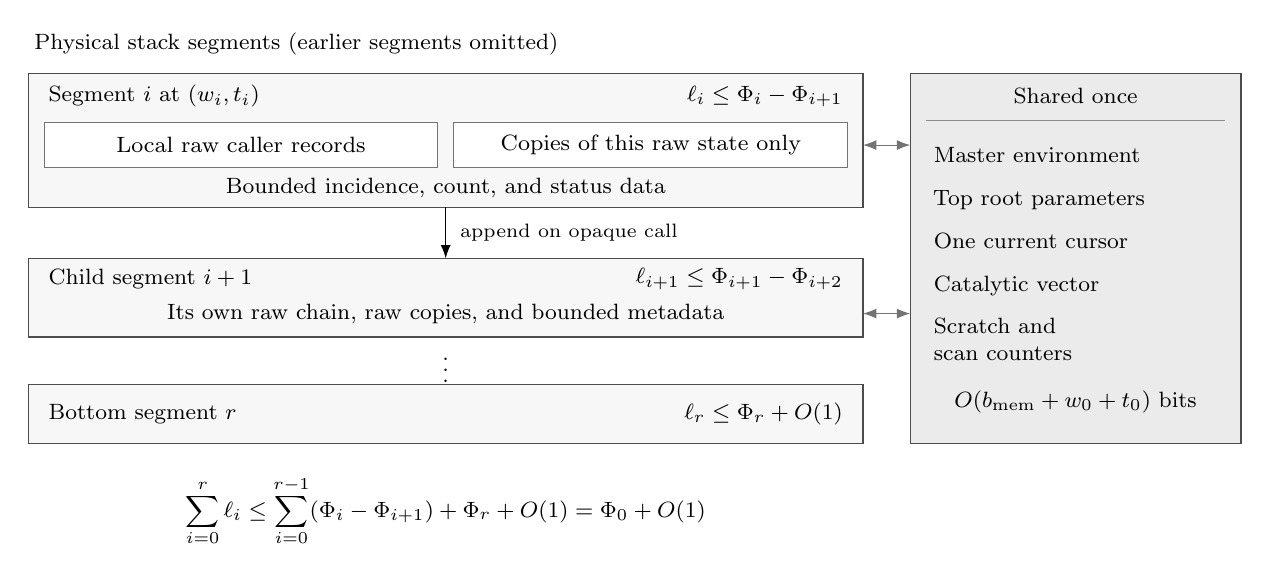
\begin{tikzpicture}[
  x=1cm,y=1cm,
  font=\footnotesize,
  every node/.style={inner sep=2pt},
  segment/.style={draw=black!70,line width=.5pt,fill=black!3},
  raw/.style={draw=black!55,line width=.4pt,fill=white},
  call/.style={-{Latex[length=1.7mm]},line width=.5pt}
]
  \node[anchor=west] at (0,5.62)
    {Physical stack segments \textnormal{(earlier segments omitted)}};

  \draw[segment] (0,3.55) rectangle (10.6,5.25);
  \node[anchor=west] at (.18,4.96) {Segment $i$ at $(w_i,t_i)$};
  \node[anchor=east] at (10.42,4.96)
    {$\ell_i\le \Phi_i-\Phi_{i+1}$};
  \draw[raw] (.2,4.05) rectangle (5.2,4.63);
  \node[align=center,text width=4.7cm] at (2.7,4.34)
    {Local raw caller records};
  \draw[raw] (5.4,4.05) rectangle (10.4,4.63);
  \node[align=center,text width=4.7cm] at (7.9,4.34)
    {Copies of this raw state only};
  \node at (5.3,3.79) {Bounded incidence, count, and status data};

  \draw[call] (5.3,3.55) -- (5.3,2.9)
    node[midway,right=3pt,font=\scriptsize] {append on opaque call};
  \draw[segment] (0,1.9) rectangle (10.6,2.9);
  \node[anchor=west] at (.18,2.64) {Child segment $i+1$};
  \node[anchor=east] at (10.42,2.64)
    {$\ell_{i+1}\le \Phi_{i+1}-\Phi_{i+2}$};
  \node at (5.3,2.2)
    {Its own raw chain, raw copies, and bounded metadata};

  \node at (5.3,1.59) {$\vdots$};
  \draw[segment] (0,.55) rectangle (10.6,1.3);
  \node[anchor=west] at (.18,.925) {Bottom segment $r$};
  \node[anchor=east] at (10.42,.925) {$\ell_r\le\Phi_r+O(1)$};

  \draw[draw=black!70,line width=.5pt,fill=black!8]
    (11.2,.55) rectangle (15.4,5.25);
  \node at (13.3,4.96) {Shared once};
  \draw[black!45,line width=.4pt] (11.4,4.65) -- (15.2,4.65);
  \node[align=left,text width=3.6cm] at (13.3,2.96) {
    Master environment\\[6pt]
    Top root parameters\\[6pt]
    One current cursor\\[6pt]
    Catalytic vector\\[6pt]
    Scratch and\\scan counters
  };
  \node[align=center] at (13.3,1.08) {$O({b_{\rm mem}}+w_0+t_0)$ bits};
  \draw[<->,>=Latex,black!55,line width=.4pt]
    (10.6,4.34) -- (11.2,4.34);
  \draw[<->,>=Latex,black!55,line width=.4pt]
    (10.6,2.2) -- (11.2,2.2);

  \node[anchor=north] at (5.3,.22) {
    $\displaystyle
      \sum_{i=0}^{r}\ell_i
      \le \sum_{i=0}^{r-1}(\Phi_i-\Phi_{i+1})+\Phi_r+O(1)
      =\Phi_0+O(1)$
  };
\end{tikzpicture}
\caption{Physical stack space, with $\ell_i$ the length of segment $i$
and $\Phi_i=\Phi(w_i,t_i)$.  Opaque child work is appended outside raw
copies.  The proved record certificates and local graph bound, with
enlarged ${a},{d_{\rm num}}$, pay for copies and metadata.  Shared facilities are
counted separately.  The displayed copies occur at traversal calls;
older physical segments are not copied into the child.  Ordinary
restoring and numerical segments obey the same difference bound.}
\label{fig:ctrl-space}
\end{figure}





The telescoping sum bounds the call records. We still have to bound shared scratch when a child asks for a later digit than its parent. The separate clock inequality in \eqref{eq:ctrl-local-bound} gives
\begin{equation}\label{eq:ctrl-clock-invariant}
 \Psi(w_{i+1},t_{i+1})\le\Psi(w_i,t_i).
\end{equation}
Since $t_i\le\Psi(w_i,t_i)$, all clocks are
$O(t_{\mathrm{top}}+w_{\mathrm{top}})$.
This also bounds the public scratch calculations in the arithmetic
theorem.  An uncharged full coefficient or cursor copy cannot persist
there: any operand-dependent early word crossing a query was included
in its record certificate, while pure public computations have no
recursive query.  The master environment, cursor, catalyst, scratch
and their global scan counters are single facilities.  Their total
space is $O({b_{\rm mem}}+t_{\mathrm{top}}+w_{\mathrm{top}})$.

For exact-stream semantics the induction is valid for each finite
requested clock, allowing scratch to scale with that clock.  Every
structural domain uses its fixed finite-margin clock, so its definition
does not change in this argument.  In particular the integer ${n}_t$ of a
score rank or arithmetic operation is always evaluated by its own
place convention, even when used in a request for the next digit.
The actual application has ${m}_{\mathrm{top}},t_{\mathrm{top}}=O({b_{\rm mem}})$,
and hence all these facilities and active records use $O({b_{\rm mem}})$ bits.
\end{proof}





% ---- sections/conclusion ----
% Pedagogical rewrite, October 8, 2026. Original mathematics: OpenAI.
\section{From the estimator to deterministic simulation}
\label{sec:conclusion}

We now put the three parts together. The exact hierarchy supplies a success contribution close to acceptance probability. The estimator approximates that success contribution for most environments. The controller evaluates every environment in logarithmic space and always halts. These statements have different quantifiers, and the final reduction needs each in its stated form.

There are three errors to allocate: the residual transition contribution, the estimator's statistical error at the designated start, and truncation of its numerical digits. We choose the parameters so that their sum is below the requested accuracy. Enumerating the conditional environments and taking a median then produces a deterministic approximation, without a promise that the acceptance probability lies outside a decision gap.

All transducers below have read-only input and a one-way write-only
output tape. Output contents are never available as work memory.
For a fixed randomized machine $\mathcal M$, write
$p_{\mathcal M}(x)$ for its acceptance probability on input $x$.

\begin{theorem}[Fixed inverse-polynomial accuracy]
\label{thm:fixed-precision}
Fix a randomized machine $\mathcal M$ with polynomial worst-case
running time and $O(\log(n+2))$ work space, and fix an integer $d\ge1$.
There is a uniform deterministic transducer that, on every input $x$
of length $n$, outputs a dyadic rational $z_x\in[0,1]$ with
\[
 |z_x-p_{\mathcal M}(x)|\le(n+2)^{-d}.
\]
Its work space and output length are $O(\log(n+2))$, and its running
time is polynomial in $n+2$. The constants may depend on
$\mathcal M$ and $d$, but not on the input.
\end{theorem}

The fixed exponent in this theorem is enough to decide bounded-error
computations. After proving it, we derive the class equality and its
promise version. We then allow the requested accuracy to be part of the
input and construct accepting computations under an inverse-polynomial
probability promise.

\begin{algorithm}[label=alg:final-median]{Deterministic probability approximation}
\textbf{Input.} A fixed resource-bounded randomized machine, an input, and a fixed inverse-polynomial error requirement.
\begin{enumerate}[leftmargin=*]
\item Build the implicit time-layered model and choose the hierarchy depth so that its deterministic residual error is within its assigned tolerance.
\item Choose the top accuracy level to pay for the target statistical error at the specified primary start. Choose the numerical digit precision separately.
\item Enumerate original environment encodings satisfying the top start-retention condition, preserving their multiplicities. For each, evaluate the final success entry to the prescribed numerical precision.
\item Find a median using repeated counting passes over those encodings. Recompute values when needed; keep no list of estimates.
\end{enumerate}
\textbf{Output.} The median approximation. The proof below allocates the errors, proves a majority of accurate estimates, and bounds every seed's computation.
\end{algorithm}

\subsection{Choose constants before choosing the input-dependent ranges}
\label{subsec:final-constants}

Several parts of the proof ask for a fixed constant to be sufficiently large or small. We record their order here to ensure that no later choice invalidates an earlier estimate. In particular, the averaging gap is uniform in the field size and number of free bits; the field can therefore be chosen after the required identifier and sampling ranges are known.

The construction has the following order of choices.
\begin{enumerate}
\item Fix ${h},h_0,s=8$ and the fixed number of independent channels.
The finite-action gap is uniform in every later modulus and bit length.
\item Choose the correction thresholds and cutoff, then the iteration
count $k_*$ from the factorial bound and its resulting uniform
magnitude constants. These estimates hold for every column multiplier
in $[0,1]$.
\item Choose ${d}_0$ for the density reduction, the routing thresholds,
and the finite ladders of entry and gate thresholds. The row-gate
rank ${k_{\rm row}}$ can then be chosen from the row-mass bounds alone.
\item Choose the detector rank ${j_{\rm det}}$ large enough for the incidence
bound on extra copies. Choose ${r}_*$ large enough for overload
detection, and finally the incoming rank ${k}_c$ large enough for
correction normalization. The earlier row-gate choice does not depend
on ${k}_c$.
\item Fix the bounded-output constant, the scale cutoff and precision
coefficient, and the prefix mean exponent. Choose the buffer
floor and capacity exponents and its noise coefficient so that all
buffer sums converge. Choose task separation and walk length
coefficients sufficiently large for the small constants in the
clean estimation induction.
\item Fix the crude range and propagation constants, then the block
gain coefficients ${d}_2,{d}_1$ and a sufficiently small rational block
width coefficient $\epsilon$. These choices close the coupled
fingerprint induction of Theorem~\ref{thm:fp-estimators}.
\item Choose the fixed operation-stratum and allowance coefficients
and the guard constants in Theorem~\ref{thm:ctrl-realization}.
Their finite enlargement does not alter the analytical tables or
the distribution of the environment.
\item Choose the coefficient of the top accuracy level, the field-size
exponent, and the minimum padding of ${b_{\rm mem}}$.
\end{enumerate}
Within each step only finitely many strict inequalities between
fixed constants are needed. The proofs in the corresponding sections
give these inequalities. In particular, the row rank is fixed before
the incoming rank, the block constants follow the crude error
constants, and the field is chosen after the reachable resource
ranges. There is no dependence of an earlier sampler gap on that
last choice.

The coefficient $\epsilon$ in this order is the fixed fingerprint
block-width coefficient. Once it has been chosen, increasing the fixed
linear top accuracy level increases the number of salt blocks but leaves the
sampler's gap uniform: all earlier salt bits form one free component in
Lemma~\ref{lem:env-gap}. The storage estimate
\eqref{eq:fp-salt-space} therefore remains $O({b_{\rm mem}})$.

For clarity, one may bound the stage index by ${l_{\rm max}}$, the inherited
suffix length by the stages remaining above a task, and logarithms
of reciprocal requested rates by
\begin{equation}\label{eq:final-admissible}
{h}{l_{\rm max}}+c({m}_{\mathrm{top}}-{m})
\end{equation}
with a sufficiently large fixed $c$. A child at slack $d$ can extend
the variable scale range by only $O(d)$ and loses at least $d$ of
accuracy level. Stage-rate resets are already covered by ${h}{l_{\rm max}}$.
The finitely many local task operations use the stated widths and
fixed subranks. Thus Equation~\eqref{eq:final-admissible} is closed
under all estimator recipes. The controller guards allow these
designated executions.

There is consequently a fixed ${c_{\mathrm{bd},p_{\rm fld}}}$ such that a prime
\[
2^{{c_{\mathrm{bd},p_{\rm fld}}}{b_{\rm mem}}}\le {p_{\rm fld}}\le 2^{{c_{\mathrm{bd},p_{\rm fld}}}{b_{\rm mem}}+1}
\]
is larger than all identifiers, makes the radix invertible, and gives
${p_{\rm fld}}2^{-k}\ge1$ for every rate ever requested. Bertrand's postulate
provides such a prime; testing consecutive integers by trial division
finds one using $O({b_{\rm mem}})$ space. The search range and running time are
$2^{O({b_{\rm mem}})}$. Field arithmetic and fixed-dimensional rank tests also
use $O({b_{\rm mem}})$ space.

\subsection{Pass from average error to the specified start}

The estimator theorem averages over source vertices. We need the value at one particular vertex, so we cannot use that theorem without paying for the loss of averaging over vertices. The next elementary calculation keeps one nonnegative summand and makes the cost explicit. Conditioning on the start being retained also identifies the exact family of environments that the deterministic algorithm will enumerate.

\begin{lemma}[Conditioning on one start]\label{lem:final-majority}
Let ${\mathbf{w}}\in[0,1]^V$, and suppose an estimator satisfies
\[
\frac1{n_{\rm v}}\mathbb E\sum_{v\in V}\frac{X_f(v)}f
 |\bar {\mathbf{w}}_{v}-{\mathbf{w}}_{v}|^8\le {c_{\rm ind}}^8 2^{-8{p_{\rm acc}}}.
\]
For any specified $z\in V$ and every $\eta>0$,
\begin{align}
\mathbb E\bigl[|\bar {\mathbf{w}}_{z}-{\mathbf{w}}_{z}|^8\mid X_f(z)=1\bigr]
 &\le {n_{\rm v}}\frac f{\pi_f}{c_{\rm ind}}^8 2^{-8{p_{\rm acc}}},
 \label{eq:final-conditional}\\
\Pr\bigl[|\bar {\mathbf{w}}_{z}-{\mathbf{w}}_{z}|>\eta\mid X_f(z)=1\bigr]
 &\le {n_{\rm v}}\frac f{\pi_f}{c_{\rm ind}}^8 2^{-8{p_{\rm acc}}}\eta^{-8}.
 \label{eq:final-tail}
\end{align}
\end{lemma}

\begin{proof}
Keep only the nonnegative summand at $z$. Since
$\Pr[X_f(z)=1]=\pi_f>0$,
\[
 \frac{\pi_f}{f}
 \mathbb E\bigl[|\bar {\mathbf{w}}_{z}-{\mathbf{w}}_{z}|^8\mid X_f(z)=1\bigr]
 =\mathbb E\!\left[\frac{X_f(z)}f|\bar {\mathbf{w}}_{z}-{\mathbf{w}}_{z}|^8\right]
 \le {n_{\rm v}} {c_{\rm ind}}^8 2^{-8{p_{\rm acc}}}.
\]
Dividing by $\pi_f/f$ proves
Equation~\eqref{eq:final-conditional}. In particular, choosing one
specified coordinate costs the factor ${n_{\rm v}}$ from the integrated norm.
Markov's inequality gives Equation~\eqref{eq:final-tail}.
\end{proof}

\begin{proof}[Proof of Theorem~\ref{thm:fixed-precision}]
We choose the hierarchy depth and accuracy level first, then convert each estimator value to a finite dyadic number. After proving that most such numbers are accurate, we explain how to find their median and count the total memory and time.

Apply Lemma~\ref{lem:model-reduction} to $\mathcal M$, with no promise
on its acceptance probability. Set
\[
 r=d\lceil\log_2(n+2)\rceil,\qquad \Delta=2^{-r},\qquad
 {l_{\rm max}}=\left\lceil\frac{{c_{\mathrm{bd},0}}{b_{\rm mem}}+r+3}{{h}-1}\right\rceil,
\]
where $|V_0|\le2^{{c_{\mathrm{bd},0}}{b_{\rm mem}}}$ is an explicit configuration bound.
Since $d$ is fixed, $r,{l_{\rm max}}=O({b_{\rm mem}})$. Let $z$ be the all-primary copy of
the start at stage ${l_{\rm max}}$. Proposition~\ref{prop:hier-reward-target}
gives
\begin{equation}\label{eq:final-hierarchy-accuracy}
 0\le p_{\mathcal M}(x)-{\mathbf{w}}_{l_{\rm max},z}\le\Delta/8.
\end{equation}
This bound holds for every acceptance probability. Choose a fixed
${c_{\mathrm{bd},n_{\rm v}}}$ large enough to bound all the resulting stage domains by
${n_{\rm v}}=2^{{c_{\mathrm{bd},n_{\rm v}}}{b_{\rm mem}}}$.

For the final success contribution task take $a=u=f=b_{l_{\rm max}}$. Its rank satisfies
$i_*=O({l_{\rm max}}+1)$, and Equation~\eqref{eq:est-precision} reads
\[
 {p_{\rm acc}}={m}_{\mathrm{top}}/{k}_{\mathrm{prec}}-{h}{l_{\rm max}}-{a}_*i_*.
\]
By Lemma~\ref{lem:env-ranks}, fix an integer ${c_{\mathrm{bd},\mathrm{tail}}}\ge1$ bounding
$(f/\pi_f){c_{\rm ind}}^8$ throughout the admissible range. Choose the fixed
linear coefficient of ${m}_{\mathrm{top}}=O({b_{\rm mem}})$ large enough that
\begin{equation}\label{eq:final-precision-choice}
 {p_{\rm acc}}\ge r+3+\frac{{c_{\mathrm{bd},n_{\rm v}}}{b_{\rm mem}}+\lceil\log_2 {c_{\mathrm{bd},\mathrm{tail}}}\rceil+3}{8}.
\end{equation}
This is the extra accuracy needed to pay the factor ${n_{\rm v}}$ in the passage to a specified vertex. The top-level and field-size choices in the preceding subsection allow this enlargement; Equation~\eqref{eq:final-admissible} still
bounds every descendant rate. Theorem~\ref{thm:fp-estimators}
supplies the success contribution moment estimate. Lemma~\ref{lem:final-majority},
with $\eta=\Delta/8$, now shows that
\begin{equation}\label{eq:final-good-environments}
 \Pr\bigl[|\bar {\mathbf{w}}_{l_{\rm max},z}-{\mathbf{w}}_{l_{\rm max},z}|>\Delta/8
       \mid X_f(z)=1\bigr]\le1/8.
\end{equation}
Thus the factor ${n_{\rm v}}$ lost on selecting one coordinate has been paid
by the statistical precision. Explicitly, the bound in
Equation~\eqref{eq:final-tail} is at most
\[
 {c_{\mathrm{bd},\mathrm{tail}}}\,2^{{c_{\mathrm{bd},n_{\rm v}}}{b_{\rm mem}}-8{p_{\rm acc}}+8r+24}\le 2^{-3},
\]
by Equation~\eqref{eq:final-precision-choice}.

We next turn the estimator values into a finite list of dyadic numbers.
For each master environment, Theorem~\ref{thm:arith-interface}
gives the digits $w_j\in\{-6,\ldots,6\}$ of its one fixed value
$\bar {\mathbf{w}}_{l_{\rm max},z}$. Structural choices do not depend on the requested
digit. Put ${k_{\rm digit}}=r+6$, compute
\[
 {a_{\mathrm{raw},\sigma}}=\sum_{j=0}^{{k_{\rm digit}}}w_j2^{{k_{\rm digit}}-j},\qquad
 a_\sigma=\min\{2^{k_{\rm digit}},\max\{0,{a_{\mathrm{raw},\sigma}}\}\},\qquad
 v_\sigma=a_\sigma2^{-{k_{\rm digit}}}.
\]
The integer ${a_{\mathrm{raw},\sigma}}$ is obtained by starting at zero and applying
${a_{\rm raw}}\leftarrow2{a_{\rm raw}}+w_j$ in order, so it uses $O({k_{\rm digit}})$ bits.
By Equation~\eqref{eq:arith-tail}, the truncation error is at most
$6\,2^{-{k_{\rm digit}}}<\Delta/8$. Clipping cannot increase error relative to
${\mathbf{w}}_{l_{\rm max},z}\in[0,1]$. Equations~\eqref{eq:final-hierarchy-accuracy}
and~\eqref{eq:final-good-environments} imply that, on more than
three quarters of the environments conditioned on $X_f(z)=1$,
\begin{equation}\label{eq:final-dyadic-accuracy}
 |v_\sigma-p_{\mathcal M}(x)|<3\Delta/8.
\end{equation}

The majority statement refers to a particular conditional distribution, so the deterministic enumeration must reproduce it exactly. Enumerate each field-matrix
entry in $\{0,\ldots,{p_{\rm fld}}-1\}$ and each raw salt bit string, retaining
precisely those encodings whose positive-degree columns form a frame
and for which $X_f(z)=1$. The retained encodings are equally weighted
and give the law in Equation~\eqref{eq:final-good-environments}.
In particular, enumerate the original salt strings, not their reduced
fingerprint parameters. Different raw strings that induce the same
fingerprint remain separate encodings; their multiplicities reproduce
the original probability law. At least one encoding is retained: a frame
exists, and its independent constant column can place the designated
evaluation in the nonempty retention box. The matrices have fixed
dimensions and $\log {p_{\rm fld}}=O({b_{\rm mem}})$; together with
Equation~\eqref{eq:fp-salt-space}, this gives $O({b_{\rm mem}})$ bits per master
environment and at most $2^{O({b_{\rm mem}})}$ encodings to enumerate.

We find the median by counting, not by storing or sorting the estimates. Let ${e_{\rm count}}\ge1$ be the number of retained encodings, found by one pass,
and let $h=\lfloor {e_{\rm count}}/2\rfloor+1$. Binary-search the integer interval
$[0,2^{k_{\rm digit}}]$ for the least $a$ such that at least $h$ retained encodings
satisfy $a_\sigma\le a$. Each count is computed by a fresh pass,
recomputing each numerator $a_\sigma$. This finds the upper median
of the finite multiset, including all repetitions. Since more than
three quarters of its members satisfy
Equation~\eqref{eq:final-dyadic-accuracy}, so does its median: fewer than
${e_{\rm count}}/4$ values can lie below the indicated interval, and fewer than
${e_{\rm count}}/4$ can lie above it. The algorithm retains only the current count
and search registers; it never stores the multiset.
Output the integers $(a,{k_{\rm digit}})$ representing $z_x=a2^{-{k_{\rm digit}}}$. Then
\[
 |z_x-p_{\mathcal M}(x)|<3\Delta/8
       \le(n+2)^{-d}.
\]

We account for the memory held during this computation. The master
environment, current cursor, catalyst, shared scratch, and suspended
controller records together use $O({b_{\rm mem}})$ bits by
Theorem~\ref{thm:ctrl-realization}, because ${m}_{\mathrm{top}},{k_{\rm digit}}=O({b_{\rm mem}})$.
The outer computation keeps only a fixed number of additional
$O({b_{\rm mem}})$-bit registers: its top parameters and designated start,
the environment enumeration index, ${e_{\rm count}}$, $h$, the current count,
the two binary-search endpoints and candidate, the digit index,
and the signed numerator accumulator. Each count is bounded by the
number of environment encodings, so it also has $O({b_{\rm mem}})$ bits.
These outer registers remain live while a digit query runs; in
particular, both its environment-enumeration state and its numerator
accumulator are included. They are present once for the whole
computation, not once per recursive level. Every query terminates on every environment,
including the inaccurate environments, by the same realization
theorem. The output is written only after the median is computed.

To bound time, use totality together with the complete configuration count. This is why termination on inaccurate environments was needed, rather than only on the majority of accurate ones. Each digit query is a halting deterministic computation with $O({b_{\rm mem}})$
work bits and physical input heads confined between the real endmarkers.
Counting its finite control, work-tape contents, and all work and input
head positions gives at most $2^{O({b_{\rm mem}})}$ complete configurations on its
fixed input. A repeated complete configuration would
force a deterministic loop, so totality bounds the query by
$2^{O({b_{\rm mem}})}$ steps. There are
$2^{O({b_{\rm mem}})}$ environment encodings, $O({k_{\rm digit}}+1)$ binary-search passes,
and ${k_{\rm digit}}+1$ digit queries per numerator. Their product is still
$2^{O({b_{\rm mem}})}=(n+2)^{O(1)}$. All finite parameters are generated
uniformly, and all constants are fixed for $(\mathcal M,d)$.
\end{proof}

\subsection{The class equality and promise separation}

\begin{proof}[Proof of Theorem~\ref{thm:main}]
Let $\mathcal M$ recognize a language in $\BPL$, with acceptance
probability at most $1/3$ on no inputs and at least $2/3$ on yes
inputs. Apply Theorem~\ref{thm:fixed-precision} with $d=3$.
For every input length, including $n=0$, its error is at most
$(n+2)^{-3}\le1/8$. Hence the dyadic answer is at most
$1/3+1/8=11/24$ on a no input and at least
$2/3-1/8=13/24$ on a yes input. Comparing this answer with $1/2$
decides the language uniformly in logarithmic space. This proves
$\BPL\subseteq\Lclass$ directly from probability approximation.

A deterministic machine may ignore its coins, giving
$\Lclass\subseteq\RL$. Two independent repetitions of an $\RL$
machine, accepting if either repetition accepts, have acceptance
probability zero on no inputs and at least $3/4$ on yes inputs.
They use logarithmic space and polynomial time, so
$\RL\subseteq\BPL$. The three inclusions prove
$\Lclass=\RL=\BPL$.
\end{proof}

A promise problem is a pair $({\mathcal{Y}},{\mathcal{N}})$ of disjoint sets of inputs.
Here $\mathsf{PromiseBPL}$, also written $\mathsf{prBPL}$,
requires one polynomial-time randomized
logarithmic-space machine that halts on every input, accepts each
input in ${\mathcal{Y}}$ with probability at least $2/3$, and accepts each
input in ${\mathcal{N}}$ with probability at most $1/3$.
The class $\mathsf{PromiseL}$ consists of pairs separated by a total
deterministic logarithmic-space decider; there is no correctness
requirement outside ${\mathcal{Y}}\cup {\mathcal{N}}$.

\begin{corollary}\label{cor:promise-bpl}
Under these conventions,
$\mathsf{PromiseBPL}=\mathsf{PromiseL}$.
\end{corollary}

\begin{proof}
The same $d=3$ approximation and threshold $1/2$ used in the preceding
proof accept every input in ${\mathcal{Y}}$ and reject every input in ${\mathcal{N}}$.
The resulting machine halts also outside the promise because its
approximation queries are total. The reverse inclusion follows by
ignoring the coins.
\end{proof}

\subsection{Handle an accuracy request supplied as input}

The fixed-accuracy theorem allows constants to depend on a fixed inverse-polynomial exponent. Theorem~\ref{thm:probability} instead needs one algorithm whose constants do not depend on the input accuracy request.

Merely asking for more digits would not achieve this: it approximates the same estimator more accurately while leaving its statistical error unchanged. We instead represent the computation as a padded input to one fixed inverse-polynomial approximator. The padding length increases the size parameter used by that approximator, while its bits can be generated on demand in the desired space.

\begin{proof}[Proof of Theorem~\ref{thm:probability}]
Fix a padded machine $\mathcal M_{\mathrm{pad}}$ as follows. On a string
beginning with $1^n0x$, where $|x|=n$, it simulates $\mathcal M(x)$
and ignores all remaining symbols. If the delimiter or the following
$n$ symbols are absent, it rejects. This is one fixed randomized
machine with polynomial worst-case running time and logarithmic work
space in its full input length. On every string with the specified
prefix its acceptance probability is $p_{\mathcal M}(x)$.
Fix once and for all the transducer of
Theorem~\ref{thm:fixed-precision} for $\mathcal M_{\mathrm{pad}}$ and $d=1$.

On input $(x,1^q)$, with $n=|x|$ and $q\ge1$, set
\[
 m=2^{q+\lceil\log_2(2n+4)\rceil+4}.
\]
Simulate that fixed transducer on the virtual length-$m$ string
\[
 y=1^n0x0^{m-(2n+1)}.
\]
An input query is answered by comparing its address with the prefix
boundaries and either returning the appropriate bit of $x$ or a
fixed bit. The simulated input-head address and all these comparisons
use $O(\log m)$ bits; the string $y$ is never stored. The simulated
transducer returns a dyadic rational $z\in[0,1]$ satisfying
\[
 |z-p_{\mathcal M}(x)|\le(m+2)^{-1}<2^{-q-4}.
\]
Its numerator and exponent have $O(\log m)$ bits and can be retained
in work space while its finite output is simulated.

Compute by exact dyadic arithmetic
\[
 a=\left\lfloor 2^{q+2}z+\tfrac12\right\rfloor.
\]
Then $0\le a\le2^{q+2}$, and rounding gives
\[
 \left|a2^{-(q+2)}-p_{\mathcal M}(x)\right|
 \le2^{-q-3}+2^{-q-4}<2^{-q}.
\]
Write the binary numerator $a$ to the output tape. It has at most
$q+3$ bits and represents the denominator specified in the theorem.
The simulator state, virtual input address, actual input counters,
captured dyadic answer, and rounding operands occupy a fixed number
of records of total size
\[
 O(\log m)=O(\log(n+2)+q).
\]
The simulation and the synthesis of each input bit take polynomial
time in $m$, so the total time is
$m^{O(1)}=(n+2)^{O(1)}2^{O(q)}$.
The padded machine and its exponent-one approximator were fixed
before reading $q$. Thus their constants are independent of the
requested accuracy. Throughout their simulation, the original size
convention is ${b_{\rm mem}}=\Theta(\log(m+2))$, exactly as required by the
estimator and controller theorems.
\end{proof}

\subsection{Construct an accepting computation from continuation values}

We return to fixed inverse-polynomial accuracy to construct an accepting
computation when the machine's acceptance probability has an
inverse-polynomial lower bound.
For a transducer, the conclusion concerns outputs certified by an
accepting run: its output tape must be write-only, so past emitted
symbols do not influence later transitions.

\begin{corollary}[Certified accepting computations]
\label{cor:certified-search}
Fix a randomized logarithmic-space machine $\mathcal M$ that halts
within a fixed polynomial bound ${\mathsf{t}}(n)\ge1$ on every input and every
coin sequence, and fix an integer $c\ge0$. There is a uniform
deterministic logarithmic-space, polynomial-time transducer that
outputs an accepting computation of $\mathcal M$ whenever
\[
 p_{\mathcal M}(x)\ge(n+2)^{-c}.
\]
On every other input it outputs either an accepting computation or
a failure symbol. If every accepting run of $\mathcal M$ emits a
valid witness for a specified relation, the transducer can instead
output such a witness with the same guarantee.
\end{corollary}

\begin{proof}
The decision approximation can also guide a path. At each configuration, some successor has continuation probability at least the current weighted average. Approximate those successor probabilities closely enough that the loss incurred by choosing the largest approximation is small over the entire path.

Give halted configurations constant self-transitions through time
${\mathsf{t}}(n)$. A configuration and its elapsed time use $O(\log(n+2))$
bits. There is a fixed randomized logarithmic-space continuation
machine which, on a valid encoding of $(x,v,t)$, starts from
configuration $v$ and simulates the remaining ${\mathsf{t}}(n)-t$ steps with
fresh coins. It checks the fixed work-space box and time bound,
rejecting malformed encodings and any attempted violation. Its
acceptance probability on the reachable configurations is the
continuation value ${\mathbf{p}}_{t,v}$, and it has a
polynomial worst-case time bound in its input length.

Write $\gamma=(n+2)^{-c}$. Choose a fixed exponent $d$ large enough
that Theorem~\ref{thm:fixed-precision}, applied to the continuation
machine, approximates every queried value within
$\delta\le\gamma/(8{\mathsf{t}}(n))$. Such a fixed exponent exists because
${\mathsf{t}}$ is a fixed polynomial and the continuation input contains $x$.
The extra fields have logarithmic length. We supply them virtually
from saved configuration and time registers, so the approximation
and those registers together use logarithmic space.

Starting at the initial configuration, at each time estimate the
continuation value of every positive-probability successor and
choose one with maximum estimated value, breaking ties by a fixed
port order. Since ${\mathbf{p}}_{t,v}$ is the weighted mean of the successor
values, the chosen successor $v'$ satisfies
\[
 {\mathbf{p}}_{t+1,v'}\ge\max_w {\mathbf{p}}_{t+1,w}-2\delta
                  \ge {\mathbf{p}}_{t,v}-2\delta.
\]
On an input satisfying the stated lower bound, after ${\mathsf{t}}(n)$ choices
the terminal continuation value is at least
$\gamma-2{\mathsf{t}}(n)\delta\ge3\gamma/4>0$. A terminal continuation value
is zero or one, so this computation accepts.

A low-probability input need not yield a successful path, so do not emit a purported accepting computation before checking where the deterministic choices lead. First run this construction without writing output. If its terminal
state rejects, output the failure symbol. Otherwise repeat the same
deterministic choices and stream the configurations through the original
first halting state, or the symbols emitted by the simulated transducer.
The artificial self-transitions after halting are omitted from the output.
This second pass follows the same accepting computation. Consequently no rejecting computation
is output, even outside the probability promise.

At any time the current, candidate, and best successor configurations,
the time counter, a constant number of dyadic scores, the virtual
input address, and the approximation workspace occupy a constant
number of $O(\log(n+2))$-bit records. The finite successor lists
have constant size, and there are only ${\mathsf{t}}(n)$ steps in each pass,
so the total running time is polynomial. Each approximation has a
deterministic guarantee at its queried configuration; no simultaneous
accuracy event for all adaptive queries is needed.
\end{proof}





\appendix

% ---- sections/arithmetic-details ----
% Pedagogical rewrite, October 8, 2026. Original mathematics: OpenAI.
\section{Detailed arithmetic constructions}

Section~\ref{sec:arith} introduced the signed-digit representation and stated the numerical guarantee used by the controller. This appendix proves the primitive operations from which that guarantee is assembled. For each operation, there are two separate questions: how accurately a finite computation approximates its exact value, and how much local information survives a request to one of its operands. We follow the same order for the elementary operations, multiplication, reciprocals, and indexed reductions.

\subsection{Compare finite truncations before taking a digit}

We first implement the elementary operations on finite truncations, and then bound their distance from the exact answer. Comparisons are between finite rational values; the algorithm never has to decide equality of two arbitrary exact reals. The truncation margin absorbs any change in which operand a maximum or minimum selects.


\begin{lemma}[Finite comparisons and bounded elementary operations]
\label{lem:arith-elementary}
The normalized operations of taking a pair average, a maximum or
minimum, and a fixed binary shift admit deterministic integers
satisfying Equation~\eqref{eq:arith-approximation}.  Their residue
procedures, for any fixed $q$, have the following properties.  There
are constants ${c_{\mathrm{bd},0}},{c_{\mathrm{bd},1}}$ such that an operand place $j$ obeys
$j\leq t+{c_{\mathrm{bd},0}}$, its suspended local record has length at most
${c_{\mathrm{bd},0}}+{c_{\mathrm{bd},1}}(t-j)$, and the intrinsic local space is $O(t+1)$.
Fixed finite compositions of these normalized operations have the
same bounds, with enlarged constants.  Fixed Boolean operations on
returned digit codes, including sign decoding and conditional selection
of code bits, add only constant local overhead.
\end{lemma}

\begin{proof}
First consider comparing two truncations through ${k_*}=t+h$, where $h$
is a sufficiently large fixed integer.  Their difference digits have
magnitude at most 12.  Scanning from place zero to ${k_*}$, update a signed
prefix by $p\leftarrow2p+\delta$.  While $|p|\leq12$, retain $p$
exactly.  Once $p>12$ or $p<-12$, retain only the corresponding
absorbing sign state.  This sign is correct for every finite
continuation: the remaining suffix, in the current scale, has
magnitude strictly less than 12.  The state space is finite, so each
transition has a fixed bounded-fan-in Boolean circuit.  The sign
at the end determines the exact order of the two finite truncations.
The path from that sign bit to an input at place $j$ has length
$O({k_*}-j+1)=O(t-j+1)$.

Let $v_t$ be the average, maximum, or minimum of the two
truncations, and put ${n}_t=\lfloor2^tv_t\rfloor$.  Each operation is
1-Lipschitz for the sup norm on its operands.  Consequently
$|v_t-v|\leq6\,2^{-{k_*}}$, where $v$ is the corresponding exact output.
Choosing $h$ so that $6\,2^{-h}<1/2$ gives
$|{n}_t-2^tv|<3/2$.

To obtain ${n}_t\bmod2^q$, only a fixed number of low places of the
selected truncation are needed.  More explicitly, at scale $2^{k_*}$,
terms of input place $j\leq t-q$ are multiples of $2^{q+h}$.
Modulo this modulus the remaining $q+h$ places suffice.  For an
average with integer input prefixes ${a}_{k_*},{b}_{k_*}$ at scale $2^{k_*}$,
use ${n}_t=\lfloor({a}_{k_*}+{b}_{k_*})/2^{h+1}\rfloor$.  Its residue needs
modulus $2^{q+h+1}$ and one additional retained place:
only places $j\leq t-q-1$ can be omitted.  The finite number
of remaining digits can be added and shifted by a constant-size
Boolean circuit.  A maximum or minimum first uses the comparison
bit to select these residue bits.  Its long comparison branch has
the path bound proved above, and its residue branch reaches only
places within a fixed distance of $t$.  A fixed shift changes these
places by a fixed amount.  Fixed normalization factors are handled
in this way whenever an intermediate range exceeds $[-1,1]$.

The topology of the comparison chain and the low-residue circuits
depends only on the root clock, the fixed margins, and the gate
path.  Regenerating a place by replaying that path needs no saved
binary place counter at each transition.  Lemma~\ref{lem:arith-gate-evaluation}
therefore gives the suspended-space bounds.  Their longest paths
have length $O(t+1)$.

For composition, use one common coefficient of $(t-j)$ for the
finite primitive list.  Increasing such a coefficient by $\Delta$
requires increasing its constant term by at most $\Delta {c_{\mathrm{bd},0}}$,
because the operand overshoot is at most ${c_{\mathrm{bd},0}}$.  With these common
coefficients, the clock differences telescope along the composed
path.  The finite number of constant terms remains a constant.
\end{proof}

We will also use the following explicit Boolean arithmetic facts.
A carry bit in binary addition is described by a generate/propagate
pair $(g,p)$.  Composition of adjacent intervals is the associative
operation
\[
 (g_2,p_2)\circ(g_1,p_1)
   =(g_2\lor(p_2\land g_1),\ p_2\land p_1).
\]
Balanced trees of these pairs give every carry in $O(\log({w_*}+1))$
depth for ${w_*}$-bit words.  A balanced tree adding ${r_*}$ such words modulo
$2^{w_*}$ has depth
\begin{equation}
 O\bigl(\log({r_*}+1)\log({w_*}+1)\bigr).
 \label{eq:arith-adder-depth}
\end{equation}
The trees can be padded by zero words to powers of two, so their
gate addresses are computable by ordinary index arithmetic.
For counts of ${r_*}$ Boolean bits one can do better: constant-depth
full adders replace three same-width rows by two rows of their sum,
with carries placed in the next column.  In $O(\log({r_*}+1))$ rounds
only two rows remain.  The word width is $O(\log({r_*}+1))$; a final
carry computation gives total depth $O(\log({r_*}+1))$.  These
constructions use bounded fan-in throughout.

\subsection{Multiply without retaining a long partial product}

Expanding a product of digit streams produces many pairs of input digits. A straightforward sum can leave a long partial result stored while requesting another digit. We instead partition the pairs according to the smaller of their two indices. In a group whose smaller index is large, both digits are early enough relative to the requested output place to pay for the circuit path leading to them.

The proof has four parts: define finite band sums, bound the omitted tails and rounding error, compute only the residues needed for the output digit, and charge each circuit path to the difference between its output and input places.

\begin{lemma}[Multiplication]
\label{lem:arith-multiplication}
For normalized exact input streams $x$ and $y$, multiplication has all
the conclusions of Lemma~\ref{lem:arith-elementary}.  In particular,
its suspended storage at an operand place $j$ is
$O(1)+c(t-j)$, despite the potentially long product expansion.
\end{lemma}

\begin{proof}
First partition the formal product and specify which pairs are retained. Fix $q$ and write ${a_*}=6$.  Partition ordered pairs $(i,j)$ of
nonnegative places into a zero band, where $\min(i,j)=0$, and
positive bands
\[
 \mathcal P_{d_*}=\{(i,j):{d_*}\leq\min(i,j)<2{d_*}\},
 \qquad {d_*}=1,2,4,\ldots.
\]
Set $h_0=h_\circ$ for the zero band and
$h_{d_*}=h_\circ+\lfloor {d_*}/4\rfloor$ for positive bands.  The fixed
integer $h_\circ$ will be chosen below.  Retain in band ${d_*}$ only
pairs with $i+j\leq t+h_{d_*}$, and let
\begin{equation}
 {s}_{d_*}=\sum_{\substack{(i,j)\in\mathcal P_{d_*}\\i+j\leq t+h_{d_*}}}
           x_i y_j2^{t+h_{d_*}-i-j}.
 \label{eq:arith-band-integer}
\end{equation}
For the zero band the same formula uses its defining pair set.
These are mathematical integers; no bound on their full binary
length is assumed in the residue computation.

The omitted tails can be bounded without forming the band sums. At any fixed diagonal $i+j=s$, a positive band contains at most
$2{d_*}$ ordered pairs.  Indeed the smaller place has ${d_*}$ possibilities,
and an off-diagonal pair has two orientations.  The zero band has
at most two pairs.  Thus, in units of $2^{-t}$, the total omitted
product terms have absolute sum at most
\begin{equation}
 E_{\mathrm{omit}}
 \leq 2{a_*}^2\sum_{{d_*}\in\{0,1,2,4,\ldots\}}({d_*}+1)2^{-h_{d_*}}.
 \label{eq:arith-band-tail-error}
\end{equation}
The geometric summation of the diagonal weights gives this bound
also when the truncation threshold lies below the first possible
diagonal.  Both the series in Equation~\eqref{eq:arith-band-tail-error}
and $\sum_{d_*}2^{-h_{d_*}}$ converge.  Choose $h_\circ$ sufficiently large
that their displayed combined error bound, including coefficient
$2{a_*}^2$, is less than $1/2$.

There are only finitely many nonempty retained bands.  For a
positive one, $2{d_*}\leq t+h_{d_*}$, whence
\begin{equation}
 {d_*}\leq\frac47(t+h_\circ).
 \label{eq:arith-last-band}
\end{equation}
The left side of the nonemptiness condition grows monotonically
faster than its right side along the dyadic bands.  We may therefore
stop at the last band satisfying this inequality, retaining empty
bands within the finite prefix if necessary.

Starting with the most distant retained band, define integers
recursively by
\begin{equation}
 {f}_{d_*}={s}_{d_*}+
       \left\lfloor 2^{h_{d_*}-h_{{d_*}^+}}{f}_{{d_*}^+}\right\rfloor,
 \qquad
 {n}_t=\left\lfloor2^{-h_0}{f}_0\right\rfloor,
 \label{eq:arith-band-recursion}
\end{equation}
where ${d_*}^+$ is the next band, and the last missing tail is zero.
One internal floor, divided back to scale $2^t$, changes the sum
by less than $2^{-h_{d_*}}$.  Induction down the bands consequently
shows that the difference between $2^{-h_0}{f}_0$ and the sum of
all retained terms in scale-$t$ units is at most $\sum_{d_*}2^{-h_{d_*}}$.
Equation~\eqref{eq:arith-band-tail-error} and the choice of
$h_\circ$ make the error before the final floor less than $1/2$.
The final floor costs less than one more unit.  Therefore
Equation~\eqref{eq:arith-approximation} holds for $z=xy$.

The integers in this recurrence define the approximation; they need not be stored in full. We next implement Equation~\eqref{eq:arith-band-recursion} using residues.  At band ${d_*}$ use modulus $2^{q+h_{d_*}}$.  An integer term
in Equation~\eqref{eq:arith-band-integer} with $i+j\leq t-q$
is a multiple of this modulus and can be omitted from the circuit.
It remains present in the mathematical integer ${s}_{d_*}$.
Only the diagonals
\begin{equation}
 t-q<i+j\leq t+h_{d_*}
 \label{eq:arith-relevant-diagonals}
\end{equation}
need to be processed, giving
$O(({d_*}+1)(h_{d_*}+q+1))=O(({d_*}+1)^2)$ candidate pairs.

Signed floor shifts are well defined on the required residues.
For $h'\geq h$ and $a-b=k2^{q+h'}$,
\begin{equation}
 \left\lfloor\frac{a}{2^{h'-h}}\right\rfloor
 -\left\lfloor\frac{b}{2^{h'-h}}\right\rfloor
       =k2^{q+h}.
 \label{eq:arith-signed-residue-floor}
\end{equation}
This identity holds for all signed integers $a,b$.  Thus a next-band
residue modulo $2^{q+h'}$ supplies the correctly floor-shifted
tail modulo $2^{q+h}$.  Apply the same observation to the final
shift by $h_0$ to obtain ${n}_t\bmod2^q$.
In the finite binary circuit, this shift just discards the lowest
$h'-h$ bits of the canonical $(q+h')$-bit residue.  The displayed
identity proves that this is valid also when the underlying integer
is negative.

For completeness, the finite gate structure can be indexed without
storing an absolute operand place at each gate.  For a positive
band enumerate triples $(r,s,o)$, where
${d_*}\leq r<2{d_*}$, $t-q<s\leq t+h_{d_*}$, and $o\in\{0,1\}$.
The triple supplies $(r,s-r)$ if $s-r\geq r$ and $o=0$;
it supplies $(s-r,r)$ if $s-r>r$ and $o=1$; otherwise it supplies
a zero term.  This enumerates the relevant pairs exactly once.
For the zero band use $r=0$ with the same orientation rule.
Negative candidate places are invalid and supply zero.
The offsets $r-{d_*}$ and $s-(t-q+1)$ have $O(\log({d_*}+2))$ bits.
They and $o$ are obtained from paths in padded binary selection trees.
The full places are then computed from the root clock in scratch.

Each nonzero term is a constant-bit signed product $x_i y_j$,
shifted into a word of width ${w}_{d_*}=q+h_{d_*}=O({d_*}+1)$ and interpreted
modulo $2^{{w}_{d_*}}$.  A bit of this word is a fixed Boolean function
of the two bounded digit codes, the bit index and the known shift;
negative products use their ordinary residue, equivalently sign
extension before reduction.  Add these words and the shifted tail
using Equation~\eqref{eq:arith-adder-depth}.  A band contributes
depth $O(\log^2({d_*}+2))$.  Bit selection for the shifted tail is
wiring and does not require evaluating a full tail word.

It remains to connect circuit depth with the digit place of an operand. This is the reason for grouping by the smaller input index. The sum of these depths through the bands up to ${d_*}$ is
$O(\log^3({d_*}+2))$, hence at most ${c_{\rm bd}}({d_*}+1)$ for a fixed ${c_{\rm bd}}$.
For an original input digit in a positive band, its partner place
is at least ${d_*}$.  Equation~\eqref{eq:arith-relevant-diagonals} gives
\begin{equation}
 j\leq t+h_{d_*}-{d_*}
       \leq t+h_\circ-\frac34{d_*}.
 \label{eq:arith-multiplication-latency}
\end{equation}
Equivalently, $t-j\geq\tfrac34{d_*}-h_\circ$, so the full path cost
through these bands satisfies
\[
 {c_{\rm bd}}({d_*}+1)\leq {c_{\rm bd}}\left(1+\frac43h_\circ\right)
                   +\frac{4{c_{\rm bd}}}{3}(t-j).
\]
This gives ${c_{\mathrm{bd},0}}+{c_{\mathrm{bd},1}}(t-j)$ with fixed constants.  The zero band
has constant depth and only constant overshoot.  All its gate
descriptions, term coordinates, bit positions and tail shifts are
computable by replaying paths and doing integer index arithmetic
from $t$ and $q$.  Lemma~\ref{lem:arith-gate-evaluation} converts these
depth bounds to suspended storage.  Finally,
Equation~\eqref{eq:arith-last-band} bounds every intrinsic path
and local word width by $O(t+1)$.
\end{proof}

\subsection{Take a reciprocal using an early prefix and a small remainder}

For a reciprocal, a prefix through roughly half the requested digit place is enough to define a linear approximation whose remaining error is quadratically small. Forming that prefix requires a long word. The memory bound is still possible because the word is present only while the algorithm queries early input places, where the output-to-input digit difference is large enough to pay for it.

The crucial order is to compute a needed coefficient digit from the early prefix, release the prefix word, and only then request a late digit of the input remainder. Treating the prefix as a permanent local constant would lose the storage bound.

\begin{lemma}[Reciprocal on a positive compact interval]
\label{lem:arith-reciprocal}
Fix constants $0<a\leq b$.  On inputs $x\in[a,b]$, a reciprocal,
after a fixed known normalization, has the same operand-clock,
suspended-record, and intrinsic-space bounds as in
Lemma~\ref{lem:arith-elementary}.  Its local record may contain an
$O(t+1)$-bit word only while querying input places
$j\leq\lfloor t/2\rfloor+O(1)$.
\end{lemma}

\begin{proof}
The input can first be normalized by a fixed binary scale.  It is
enough to prove the result with a fixed digit alphabet and fixed
positive interval; all constants below may depend on $a,b$.
Choose a fixed power of two ${c_{\rm bd}}$ large enough that the desired output
$z=1/({c_{\rm bd}}x)$ lies in $[0,1]$ and that the coefficients below have
absolute value at most one.  Put
\[
 k=\lfloor t/2\rfloor+c,\qquad x^0=x^{[k]},\qquad e=x-x^0,
\]
where $c$ is a sufficiently large fixed integer.  By
Equation~\eqref{eq:arith-tail}, $|e|\leq 6\,2^{-k}$.  Choosing $c$
first ensures $x^0\in[a/2,2b]$ and $|e|\leq1$ at every $t$.
Increasing ${c_{\rm bd}}$ if necessary gives bounded coefficients
\[
 \alpha=\frac1{{c_{\rm bd}}x^0},\qquad \beta=-\frac1{{c_{\rm bd}}(x^0)^2}.
\]
The exact algebraic identity
\begin{equation}
 \frac1{{c_{\rm bd}}x}=\alpha+\beta e+
               \frac{e^2}{{c_{\rm bd}}(x^0)^2x}
 \label{eq:arith-reciprocal-taylor}
\end{equation}
shows that the linear expression ${t}_t=\alpha+\beta e$ differs
from $z$ by at most a fixed constant times $2^{-2k}$.
Choose $c$ large enough that
\begin{equation}
 2^t|{t}_t-z|\leq\frac14
 \quad\hbox{for every }t\geq0.
 \label{eq:arith-reciprocal-remainder}
\end{equation}
Clipping ${t}_t$ to $[-1,1]$ cannot increase this error; denote the
clipped expression by $\widehat {t}_t$.

For this fixed original $t$, the coefficients $\alpha,\beta$ are
exact rational numbers.  Their digits are produced by integer
arithmetic, as described below.  The suffix $e$ has the exact stream
with digit zero through $k$ and digit $x_j$ thereafter.  Thus
Lemmas~\ref{lem:arith-elementary} and
\ref{lem:arith-multiplication} provide exact streams for
$\widehat {t}_t$, using only a fixed number of normalized operations.
Explicitly, form the product $\beta e$, then the pair average
$u=(\alpha+\beta e)/2$, clip $u$ to $[-1/2,1/2]$ by a maximum
and a minimum, and finally apply the fixed shift by 2.  Every
exported intermediate value is normalized, and the final value is
$\widehat {t}_t$.  Forming this expression introduces no additional
reciprocal operation.

Let ${p}_s(\widehat {t}_t)$ be the integer approximation furnished by
those operations at place $s=t+3$, and define
\begin{equation}
 {n}_t(z)=\left\lfloor {p}_{t+3}(\widehat {t}_t)/8\right\rfloor.
 \label{eq:arith-reciprocal-approximation}
\end{equation}
The cutoff $k$ and the coefficients remain those of the original $t$,
not those of $s$.  Equations~\eqref{eq:arith-approximation} and
\eqref{eq:arith-reciprocal-remainder} give
\[
 |{n}_t(z)-2^tz|<1+\frac28+\frac14=\frac32<2.
\]
To obtain this integer modulo $2^q$, ask for the approximation
${p}_{t+3}$ modulo $2^{q+3}$ and use
Equation~\eqref{eq:arith-signed-residue-floor}.

The approximation error is now controlled. We separately verify the lifetime of the operand-dependent words, since their rational form alone does not make them public constants. It remains to justify storage in the coefficient computations.
The signed numerator of $x^0$ in units $2^{-k}$ has $O(k+1)$
bits.  Form it by querying places $0,\ldots,k$ and updating the
integer prefix.  The numerator, a place counter, and all data that
must survive the next query are part of the local record.
To return a coefficient digit of place $r$, numerator squaring and
integer division require $O(k+r+1)$ bits.  Here $r\leq t+O(1)$,
because the enclosing expression has fixed depth and constant
overshoot.  After the input prefix is obtained, these integer
computations make no further operand queries.  Standard binary
long multiplication and division, performed by bounded loops with
their partial products or remainder, use only this linear number
of bits.  For $r>0$, computing floors of the coefficient scaled at
$r$ and $r-1$ gives its exact difference digit; at $r=0$ use the
place-zero floor alone, as in Lemma~\ref{lem:arith-residue-stream}.
Clipping is unnecessary
because the coefficients were normalized in advance.

Every original-input query during this formation has
$j\leq k\leq t/2+O(1)$.  Hence
\begin{equation}
 t+1\leq {c_{\mathrm{bd},2}}+{c_{\mathrm{bd},3}}(t-j)
 \label{eq:arith-early-word-payment}
\end{equation}
for fixed constants, at all such queries.  The enclosing gate path
also has length $O(t+1)$, so the complete suspended local record
satisfies the required bound there.  Equivalently, the coefficient
branch is charged against the original reciprocal clock $t$, not
against its possibly small coefficient digit place $r$.

On a suffix branch with $j>k$, the coefficient word is absent.
The Boolean evaluation asks for a coefficient digit at a separate
leaf, returns its bounded code bits, and discards the coefficient
word.  If the other child of a gate subsequently asks for a late
suffix digit, only the bounded pending bits and gate choices are
retained.  The path bound from the preceding arithmetic lemmas
therefore gives $O(1)+c(t-j)$ also on this branch.  Repeated
coefficient requests rebuild the word.  The parameter $k$ and the
choice of coefficient are regenerated from the original $t$ and
the saved gate path; no earlier cursor address is required.
All intrinsic records have $O(t+1)$ bits.
\end{proof}

The coefficients in this proof are operand-dependent, even though they
are rational once $x^0$ is known.  They therefore do not qualify as
public coefficient leaves.  A coefficient request first forms its
charged early prefix, then uses scratch for integer arithmetic, returns
only the requested bounded digit, and releases that prefix before a
suffix branch is evaluated.  The original reciprocal clock $t$ remains
regenerable throughout.  This order of operations is the lifetime rule
used in the suspended-record bound.  In particular, $j\le\lfloor t/2\rfloor+c$
gives the explicit payment $t+1\le2(t-j)+2c+1$ for the early word.

\subsection{Order statistics, sums, and finite-accuracy access tests}

The remaining operations have an explicitly indexed domain of size at most exponential in the local descriptor length. We can recompute a value whenever it is compared or added, rather than store the whole domain. Numerical order statistics may select different approximating entries at different digit places, but they must approximate one fixed exact order statistic. By contrast, a structural access test has a fixed precision chosen once for that test.

\begin{lemma}[Indexed finite ranks]
\label{lem:arith-rank}
Fix $\kappa>0$ and $d\geq1$.  Consider at most $2^{\kappa d}$
normalized values, indexed by descriptors of length at most
$\kappa d$, and an order statistic specified by an $O(d)$-bit
index.  The semantic list length $n$ is public; the requested index
is in $\{1,\ldots,n\}$, or an out-of-range request returns a
prescribed normalized constant.  Absent descriptors may be assigned
prescribed constant dummy values by structural validity predicates.
This order statistic has deterministic integer approximations ${n}_t$
satisfying Equation~\eqref{eq:arith-approximation}.  Their residue
procedures have constants $a,b,c$, depending only on the descriptor
bounds, such that an operand digit query at $j$ obeys
\begin{equation}
 j\leq t+cd,\qquad
 {l_*}\leq ad+b(t-j),
 \label{eq:arith-local-bound}
\end{equation}
where ${l_*}$ is the total suspended local record length.  A structural
validity query is assigned clock zero and has suspended length
$O(d+t)$.  The intrinsic local length is $O(d+t)$.
\end{lemma}

\begin{proof}
For $1\le k\le n$, the $k$th largest of the semantic $n$-entry list
is its $(n-k+1)$st ascending order statistic, before any extra padding.
Pad to a fixed descriptor domain whose cardinality is a power of
two, adding entries of value $+1$.  These entries do not change
any of the first $n$ ascending order statistics.  An empty list or
an out-of-range request returns its specified default immediately.
Replace invalid original descriptors by the prescribed dummies.
An operand access evaluates validity first and enters the actual
value branch only when valid; an invalid access returns the dummy's
digit.  Thus a dummy does not require a query to an undefined value.
For each valid numerical value use its truncation through
${k_*}=t+h$ for fixed large $h$.  Order these finite rational values,
breaking ties by descriptor index.  Compare every pair using the
signed comparison of Lemma~\ref{lem:arith-elementary}.  For each
descriptor count how many descriptors precede it, then compare
that count to the requested rank minus one.  Exactly one
descriptor is selected.  Select its low-residue bits using Boolean
AND and OR trees and finally floor to output scale $2^t$.
The selected descriptor is internal to this residue computation.  It
may change with $t$; the exact order statistic being approximated is
fixed by the semantic list and the requested index.

If all coordinates of two finite lists differ by at most $\eta$,
their corresponding order statistics differ by at most $\eta$.
Indeed, at least the specified number of the perturbed entries
are no larger than the original order statistic plus $\eta$;
interchanging the lists gives the reverse inequality.  Here
$\eta=6\,2^{-{k_*}}$.  Thus the selected truncation, followed by the
final floor, satisfies Equation~\eqref{eq:arith-approximation}
for sufficiently large fixed $h$.  Descriptor ties affect neither
this estimate nor the uniqueness of the finite selection.
This argument perturbs the entire padded exact list.  Some truncated
original entries may exceed $+1$ slightly, but their error, and hence
the error of the selected padded order statistic, is still at most
$\eta$.  The padding argument requires no separate claim that every
finite truncation remains in $[-1,1]$.

Each count has $O(d)$ bits.  Carry-save counting as described
above, the comparison to the requested rank, and selection among
$2^{O(d)}$ descriptors add $O(d)$ Boolean depth above the
pairwise comparison bits and selected residue bits.  A
place-$j$ input to a pairwise comparison consequently has path
length $O(d)+O(t-j)$; a residue input is within a fixed distance
of $t$ and has path length $O(d)$.  The paths to validity predicates
have length at most the whole circuit depth $O(d+t)$, and the
predicates themselves are separate structural leaves of clock zero.

Each gate is specified by its pair of descriptor indices, its
counting-tree or selection-tree position, and a comparator or bit
position.  The paths determine these indices in $O(d+t)$ scratch,
using only the fixed domain and root parameters.  No numerical
comparison is needed to determine the circuit topology.  Apply
Lemma~\ref{lem:arith-gate-evaluation}.  The constants in
Equation~\eqref{eq:arith-local-bound} can absorb the fixed digit
overshoot because $d\geq1$.
\end{proof}

For the compression ranks, copies of a previously computed baseline
are ordinary indexed operands: their digit interfaces query the
baseline's exact stream one bounded digit at a time.  A slot that
chooses between an entry and the baseline first evaluates its
structural flag and then queries the selected, already-defined stream.
Treating this as a defined operand interface leaves no absent value
for the rank procedure to evaluate.
The required baseline copies belong to the semantic list; the extra
power-of-two padding in the proof is then supplied by the constant
$+1$.  The structural choice adds only a fixed conditional branch,
so the same digit-clock and suspended-record bounds apply.

A rank over the full incoming vertex universe need not have a $2^{O(d)}$ descriptor domain. That operation uses the terminal-program construction of Lemma~\ref{lem:ctrl-score-rank}, rather than the finite-domain result proved here.

A sum is evaluated by a balanced tree of normalized pair averages, followed by a known scale adjustment. This avoids retaining a sequential accumulator across late operand queries. The number of tree levels is paid for by the descriptor length.

\begin{lemma}[Bounded sums and known scales]
\label{lem:arith-sums-scales}
Suppose an immediate descriptor domain has at most $2^{\kappa d}$
terms, all required binary scale exponents have magnitude at most
$\kappa d$, and every intermediate output has a known range bound
$2^{\kappa d}$.  A sum over an empty domain is zero, and an average
is taken over a public nonempty domain.  Balanced sums or averages of these terms, followed
by the required known rescalings and bounded clipping, satisfy
Equation~\eqref{eq:arith-local-bound} and have intrinsic local
space $O(d+t)$.
\end{lemma}

\begin{proof}
Choose one common known power-of-two range bound for the immediate
terms and divide each term by it, so every term lies in $[-1,1]$.
Pad their number to a power of two $2^r$, $r=O(d)$, and use a complete
binary tree of pair averages.  Every internal value stays normalized.
Along one path there are $r$ elementary operations.  Choose common
coefficients in their bounds, as in the last paragraph of the
proof of Lemma~\ref{lem:arith-elementary}.  The constant terms
sum to $O(r)$ and the differences of successive digit clocks
telescope.  Thus the local length is $O(d)+b(t-j)$ and the
total overshoot is $O(d)$.  Restore the common normalization scale
only after the tree of pair averages.  For a sum, combine this factor
with the known padding count $2^r$ in one binary shift of magnitude
$O(d)$.  For an average over an original domain of size $m$, combine
the scale restoration with multiplication of the padded average by
the public factor $2^r/m$.  With minimal padding the latter factor
is in $[1,2)$, so it requires only one normalized public multiplication
and a fixed shift in addition to the common scale restoration.

More explicitly, for a shift by $2^v$, truncate the operand at
${k_*}=\max(0,t+v+h)$.  If $t+v+h\geq0$, its scaled truncation
error in scale-$t$ units is at most $6\,2^{-h}$.  If the scaled
output is known to be normalized, floor in the desired output
scale.  Otherwise, when a bounded clip is required, apply that
clip to the scaled truncation before flooring.  For the
normalized clip to $[-1,1]$, for example, define the approximation
using $\min(1,\max(-1,2^v x^{[{k_*}]}))$; its error cannot increase.
This shift-and-clip procedure does not first export an unbounded
intermediate as a normalized stream.
The low residue requires the constant number of places near
$t+v$, and a comparison needed for clipping has a constant-state
chain through ${k_*}$.  Comparisons to the scaled clipping endpoints
are equivalently comparisons of $x^{[{k_*}]}$ to the known endpoints
divided by $2^v$; their finite constants and shifted place data
are public.  When $v\geq0$ these endpoints belong to $[-1,1]$;
when $v<0$ the normalized operand is already in the clip interval
after scaling, so no clipping comparison is needed.  Its path cost is
$O(1)+O(\max(0,t+v-j))$, which is at most
$O(d)+O(t-j)$ on an actual operand query.  If $t+v+h<0$, zero
is already a sufficiently accurate approximation after increasing
$h$, and no operand query is needed.  A fixed number of such
rescalings and clips preserves the bounds by telescoping.
Known non-power-of-two coefficients can instead be handled as
public normalized streams and bounded multiplication.
\end{proof}

An access decision does not need to distinguish values exactly at one sharp threshold. The allowed gap between acceptance above $2u$ and rejection at or below $u$ makes a fixed finite precision sufficient. This is the numerical basis for the support margins used in the table and compression constructions.

\begin{lemma}[Finite buffered tests]
\label{lem:arith-buffered-test}
Let $d\geq1$, let $s$ and $u$ have known magnitude bound $2^{\kappa d}$,
and suppose $u\geq\rho\geq2^{-\kappa d}$.  There is a deterministic
finite test that accepts every $s>2u$ and accepts only $s>u$.
It uses $O(d)$-place digit queries after normalization, with
intrinsic and suspended local lengths $O(d)$.  Its result is
independent of any subsequent numerical output clock.
\end{lemma}

\begin{proof}
Compute finite rational approximations $\widetilde s,\widetilde u$
with individual errors at most $\rho/16$.  The known range and
lower bound on $\rho$ make $O(d)$ normalized digits sufficient.
Accept exactly when
$\widetilde s>\tfrac32\widetilde u$, using a fixed convention
at equality.  If $s>2u$, the left side minus the right side is
greater than $u/2-5\rho/32>0$.  If $s\leq u$, it is at most
$-u/2+5\rho/32<0$.  The finite comparison and all previous
arithmetic have the bounds already proved.  The test chooses its
precision from $d$ and $\rho$, not from an enclosing numerical
clock.  With its structural starting clock defined as zero, its
operand requests have $j=O(d)$; increasing $a$ in
Equation~\eqref{eq:arith-local-bound} pays also for the term $-bj$.
\end{proof}





% ---- sections/compiler ----
% Pedagogical rewrite, October 8, 2026. Original mathematics: OpenAI.
\section{Compile a supplied machine into a deterministic simulation}
\label{sec:compiler}

The approximation theorem begins by fixing a randomized machine. There is a separate uniformity question: can one algorithm take a machine description and its supplied resource bounds, and output a deterministic simulator together with explicit bounds for that simulator? This appendix gives that compiler.

The supplied time, space, and error bounds are hypotheses about the source. The compiler does not decide whether they are true. Instead, it uses one fixed resource-capped interpreter and one fixed deterministic approximator for that interpreter. Source-dependent padding puts every promised source computation within the interpreter's caps.

\begin{theorem}[Effective simulation with explicit bounds]
\label{thm:effective-simulation}
There is a terminating algorithm which, given a finite randomized machine
description ${\mathcal{M}}$ and positive integers $a,b$, emits a deterministic
machine ${\mathcal{D}}_{\mathcal{M}}$ and positive integers ${k_{\rm space}},{h},c$ with the following guarantee.
If, on every input of length $n$ and every random tape, ${\mathcal{M}}$ halts within
$(n+2)^a$ steps, uses at most $b\lceil\log(n+2)\rceil$ work bits, and
has acceptance probability at most $1/3$ on no inputs and at least
$2/3$ on yes inputs, then ${\mathcal{D}}_{\mathcal{M}}$ decides the same language. On each input,
that same execution uses at most ${k_{\rm space}}\log(n+2)$ work bits and
${h}(n+2)^c$ elementary bit operations.
\end{theorem}

The compiler's own running time need only be finite, and its output
exponent may depend on the source.

The proof has four steps. Construct a single interpreter with unconditional resource bounds on every encoded input. Apply the approximation theorem to it once. Encode any promised source run as a sufficiently padded input to that fixed approximation program. Finally, generate the virtual-input routines and derive explicit bounds from their finite descriptions.

We prove Theorem~\ref{thm:effective-simulation} by specializing one fixed deterministic program. First we construct a randomized interpreter
${\mathcal{U}}$ that enforces polynomial-time and logarithmic-space bounds on every
input. Theorem~\ref{thm:fixed-precision} supplies a deterministic machine
${\mathcal{A}}$ that separates the inputs on which ${\mathcal{U}}$ accepts with probability at
least $2/3$ from those on which it accepts with probability at most
$1/3$. Both ${\mathcal{U}}$ and ${\mathcal{A}}$ are fixed before the compiler receives a source
description ${\mathcal{M}}$ and bounds $a,b$.

When the source satisfies its supplied resource bounds, padding places
each encoded computation within ${\mathcal{U}}$'s caps without changing its
acceptance probability. The generated machine runs ${\mathcal{A}}$ on that padded input, generating each requested
symbol from the real input. We then compute the output bounds ${k_{\rm space}},{h},c$
from the generated finite transition table and the fixed library data.
The compiler never has to select a new probability approximator or infer
resource bounds from the source's behavior.

Universal deterministic estimation has a substantial antecedent in
Pyne, Raz and Zhan~\cite[full version, Theorem~5.1]{PyneRazZhan2023}.
They construct one deterministic algorithm that, on input $(1^n,\mathcal B)$
with $n\ge1$ and $\mathcal B$ an ordered branching program of length
and width at most $n$, approximates its acceptance probability to error less than
$1/n$. For every space-constructible ${\mathsf{s}}(n)\ge\log n$, this single
algorithm uses $O({\mathsf{s}}(n))$ space exactly when
$\mathsf{prBPL}\subseteq\mathsf{SPACE}[O({\mathsf{s}}(n))]$.
Here the preceding sections establish the separator used by one fixed
library, and we compute explicit resource bounds for its source-specific
specialization.

All quantities in this section are local to the compiler construction.
In particular, ${p}$ is a padding exponent, $d_{\mathrm{code}}$ is a program
length, ${b}_n=\lceil\log_2(n+2)\rceil$, and ${n}_{\mathrm{pad}}$ is a virtual
input length.  They do not denote the accuracy levels, field modulus,
or domain sizes used in the preceding sections.  We use the usual
counted-cell convention for work tapes: traversed writable cells count
toward space, whether or not they contain a nonblank symbol.  The finite
control and the read-only input have their standard treatment.

\subsection{An interpreter that enforces its own resource limits}
\label{subsec:compiler-interpreter}

The interpreter must be small-space even on malformed or maliciously large descriptions. It therefore measures the whole input first, checks the code length before allocating storage, and imposes explicit time and tape limits during simulation. The coding below makes those checks finite scans of listed data.

Fix a binary coding of ordinary finite transition lists.  One concrete
choice uses a fixed record grammar and the field encoding
$w\mapsto 1^{|w|}0w$.  Lists specify the finite state set, tape and
alphabet declarations, initial and halting states, blanks and endmarkers,
and transition records.  A transition record lists its tested state,
scanned symbols and coin pattern, followed by its next state, written
symbols and local head movements.  The grammar has fixed nesting depth;
its fields are actual listed data, not recursively executable descriptions.
State and symbol IDs are canonical binary integers used only as names.
The first matching transition is
used; a missing transition causes rejection.  Wildcards for ignored coins
can equivalently be expanded into a finite explicit list.

Write $z$ for a program in this coding and
$d_{\mathrm{code}}=|z|\ge1$.  The coding permits at most
$d_{\mathrm{code}}$ work tapes and a block of at most
$d_{\mathrm{code}}$ fresh fair bits per simulated transition.  Every ID
has at most $d_{\mathrm{code}}$ bits.  A harmless padding field can enlarge
the program to meet these inequalities.  All tape movements are local.
Work coordinates are measured from their initial origins; the ordinary
model has one input head and one head per work tape.  For a source input
$x$ of length $n$, let ${\mathsf{E}}_{d_{\mathrm{code}}}(x)$ encode each of its
symbols by its ID padded to exactly $d_{\mathrm{code}}$ bits.

\paragraph{Preserving the supplied source bounds.}
An ordinary source machine ${\mathcal{M}}$ can be converted effectively to this format
by renaming its states and symbols and listing its transitions.  Its tapes
are represented directly, so a source transition retains its work writes
and head movements and counts as one interpreted transition.  The
conversion does not pass through a slower single-tape simulation.

Under the optional one-way read-only random-tape convention, the source
may reuse its current random bit. Store a cached bit and a validity flag
in finite control, initially invalid.
At each transition obtain one fresh bit.  Use it if the cache is invalid;
otherwise use the cached bit and discard the fresh one.  Execute the
source transition, then retain the used bit if the random head stayed
and invalidate the cache if it advanced.  This samples a newly visited
random cell lazily on its next use.  It preserves the joint distribution
of the source run and needs no initialization transition.  An initially
halting state is recognized before the first transition.  The same
argument uses a fixed finite block for a convention allowing finitely
many fresh bits per elementary transition, discarding unused bits.
The finite cache changes neither counted work space nor the number of
source transitions.  Thus the supplied parameters $a,b$ remain valid;
only the static description length can increase.

\begin{lemma}[A total resource-capped interpreter]
\label{lem:compiler-interpreter}
There is one fixed randomized Turing machine ${\mathcal{U}}$ with polynomial
worst-case running time and $O(\log(m+2))$ counted work bits on every
binary input of length $m$, with the following behavior.
Set
\begin{equation}\label{eq:compiler-interpreter-cap}
 \lambda_m=\lceil\log_2(m+2)\rceil,
 \qquad
 {\mathsf{r}}(m,d_{\mathrm{code}})
   =\left\lfloor\frac{\lambda_m}
       {100(d_{\mathrm{code}}+1)^3}\right\rfloor.
\end{equation}
On an input with prefix
\begin{equation}\label{eq:compiler-prefix}
  1^{d_{\mathrm{code}}}0\,z\,1^n0\,
  {\mathsf{E}}_{d_{\mathrm{code}}}(x),
\end{equation}
it first requires $1\le d_{\mathrm{code}}\le\lambda_m$ and
${\mathsf{r}}(m,d_{\mathrm{code}})\ge1$.  It then simulates the encoded machine
for at most $m$ transitions, allowing each counted work tape only
coordinates in $[-{\mathsf{r}},{\mathsf{r}}]$.  It rejects malformed data, a requested move
outside these bounds, or failure to halt by the end of the transition
limit.  Otherwise it returns the encoded machine's decision.  The
suffix after the complete prefix has no parsing significance.
\end{lemma}

\begin{proof}
First validate the input before allocating any description-dependent storage. Count $m$ before interpreting the prefix.  Scan the unary code-length
header with a bounded counter, rejecting if its length exceeds
$\lambda_m$ or the required delimiter is absent.  Check the two
eligibility conditions before copying $z$ or allocating simulation
storage.  Then verify that the following $d_{\mathrm{code}}$ code bits,
the unary data-length header, and the required data bits are present.
The parsed $n$ is at most $m$, and
$d_{\mathrm{code}}n\le\lambda_m m$, so even size calculations preceding
a failed length check use only $O(\lambda_m)$ bits.  List counts, ID
lengths, tape declarations, and movements are checked against the actual
code and the stated bounds before any loops or allocations using them.
There is no enumeration of an implicit domain of symbol or state names.

The eligibility conditions now imply a simultaneous storage bound for all encoded tapes and administrative records. Store the encoded tapes sequentially on a fixed number of real work
tapes of ${\mathcal{U}}$.  At most $d_{\mathrm{code}}$ strips, each with $2{\mathsf{r}}+1$
cells of $d_{\mathrm{code}}$ bits, require
\begin{equation}\label{eq:compiler-interpreter-space}
 d_{\mathrm{code}}^2(2{\mathsf{r}}+1)=O(\lambda_m)
\end{equation}
bits.  Indeed, eligibility gives
$d_{\mathrm{code}}^3\le\lambda_m$ and
$d_{\mathrm{code}}^2{\mathsf{r}}\le\lambda_m$.
The copied program, current state, scanned and written symbol tuples,
coin block, strip coordinates, step counter, and parsing scratch fit
simultaneously in $O(\lambda_m)$ bits.  A single simulated input-head
coordinate has magnitude $O(m)$ by the transition cap and therefore
also uses $O(\lambda_m)$ bits.  Read the corresponding source symbol
by rescanning the encoded data, supplying the appropriate markers or
off-data blanks according to the encoded input-tape convention.

All routines are bounded scans and ordinary binary arithmetic.  They
iterate over actual code positions, input positions, a bounded tape/head
list, strip positions, and bit positions, with a fixed nesting depth.
Each range is polynomially bounded in $m+2$; binary arithmetic is
implemented by bit scans, not unit-cost operations on growing words.
Matching a listed transition, fetching input symbols, updating the
strips, and obtaining its finite coin block therefore take polynomial
time in $m+2$, with one fixed exponent determined by these routines.
The same bounds hold when a check fails.  There are at most $m$
interpreted transitions.  Checking the initial halting state and the
state reached by the last permitted transition gives the asserted
total behavior, including $m=0$.  The resulting fixed ${\mathcal{U}}$ has the
required polynomial worst-case time on every random tape.
\end{proof}

No bounded-error language promise is asserted for ${\mathcal{U}}$ on arbitrary
inputs.  Its acceptance probability may lie between $1/3$ and $2/3$.
This is why we use probability approximation rather than a bare
language-class containment.

\subsection{Fix the deterministic approximator once}
\label{subsec:compiler-library}

The interpreter need not itself decide a bounded-error language on arbitrary encodings. This causes no difficulty because our theorem approximates arbitrary acceptance probabilities. Apply Theorem~\ref{thm:fixed-precision} to the fixed machine ${\mathcal{U}}$ and
accuracy exponent $3$, and compare its dyadic answer with $1/2$.
The error on an input of length $m$ is at most
$(m+2)^{-3}\le1/8$.  Hence the resulting deterministic machine accepts
whenever $\Pr[{\mathcal{U}}\text{ accepts}]\ge2/3$ and rejects whenever that
probability is at most $1/3$, since
\[
 \frac13+\frac18=\frac{11}{24}<\frac12
   <\frac{13}{24}=\frac23-\frac18.
\]
It halts on every input, including inputs between the two thresholds,
as also stated in Corollary~\ref{cor:promise-bpl}.  Its logarithmic
space bound counts all simultaneously live work in the approximation
algorithm.  Store the $O(\log(m+2))$-bit dyadic output in work space
for the threshold test.

We fix this library once in the following convenient form.  It is an
ordinary finite-tape deterministic decision machine ${\mathcal{A}}$ with one input
head confined to the endmarked input, initially at its left endmarker,
such that every work head stays in
\begin{equation}\label{eq:compiler-library-box}
 [-(\lambda_m+1),\lambda_m+1]
\end{equation}
relative to its origin.  To obtain this form, first consolidate any
input heads by keeping their coordinates in logarithmic work space
and scanning for each read.  Even an off-data coordinate under an
unbounded-input convention has logarithmic length because the original
library has polynomial running time.  A fixed change of initial control
state handles its input-head start convention.

Next choose an integer $w$ at least a coefficient bounding each counted
work head's distance from its origin by $w\lambda_m$.  Such one fixed
$w$ exists from the logarithmic bound, enlarged if necessary for the
finitely many small lengths.  Group consecutive work cells into blocks
of width $w$, storing within-block offsets in finite control.  The
resulting finite alphabet and finite transition list realize
Equation~\eqref{eq:compiler-library-box}, also for two-sided tapes.
All symbol widths will be charged in bits below; grouping only exposes
a uniform address bound and gives no uncharged bit compression.

This choice of ${\mathcal{A}}$, including its one blocking width, precedes every
compiler input.  More formally, the remaining construction is a
computable syntactic function of a finite library list and
$({\mathcal{M}},a,b)$.  Fixing one valid finite list yields one ordinary
computable compiler on all those source inputs.  It does not require
an algorithm that discovers a separator or a logarithmic-space
coefficient from an arbitrary machine description.  The existence
of the fixed list was proved by Theorem~\ref{thm:fixed-precision};
no constant is selected as a noncomputable function of the source
machine or its ordinary input.

The fixed finite data are the program grammar, the transition list of
${\mathcal{A}}$ with its blocked work alphabets and head conventions, and the
finite callback templates described below. The construction constants,
cutoffs, generator choices and finite instruction routines used by the
separator are included in that list. Its blocking width is fixed at
the same time. These are data specifying one compiler; subsequent
source-dependent integers are computed from these data and the supplied
$({\mathcal{M}},a,b)$.

\subsection{Use padding to fit the promised source computation}
\label{subsec:compiler-padding}

The deterministic approximator is now fixed, independently of the source description. We enlarge its virtual input enough that the interpreter's work strips and transition limit contain every promised source run. No branch of such a run is cut off, so acceptance probability is preserved exactly.

Given the source description and its supplied positive integers $a,b$, construct $z$ as above and compute
\begin{equation}\label{eq:compiler-padding}
 \begin{split}
 {p}&=1000(d_{\mathrm{code}}+2)^4(a+b+2),\\
 {b}_n&=\lceil\log_2(n+2)\rceil,
 \qquad {n}_{\mathrm{pad}}=2^{{p}{b}_n}.
 \end{split}
\end{equation}
The generated machine will run ${\mathcal{A}}$ on a virtual binary input
$y_x$ of length ${n}_{\mathrm{pad}}$ whose prefix is
Equation~\eqref{eq:compiler-prefix} and whose remaining bits are zero.
Its prefix length is exactly
\begin{equation}\label{eq:compiler-prefix-length}
 {l}_{\mathrm{pre}}
 =(d_{\mathrm{code}}+1)+d_{\mathrm{code}}+(n+1)
       +d_{\mathrm{code}}n
 =(d_{\mathrm{code}}+1)(n+2).
\end{equation}
Since ${b}_n\ge1$, $2^{{b}_n}\ge n+2$, and
$2^{{p}-1}\ge d_{\mathrm{code}}+1$, this length is at most
${n}_{\mathrm{pad}}$.  The interpreter's length parameter is
\begin{equation}\label{eq:compiler-padded-log}
 \ell_{\mathrm{pad}}
 :=\lambda_{{n}_{\mathrm{pad}}}={p}{b}_n+1.
\end{equation}

All eligibility checks pass.  In particular,
\[
 \frac{{p}}{100(d_{\mathrm{code}}+1)^3}
 =10\frac{(d_{\mathrm{code}}+2)^4}
          {(d_{\mathrm{code}}+1)^3}(a+b+2)
 \ge30(a+b+2),
\]
so
\begin{equation}\label{eq:compiler-strip-slack}
 {\mathsf{r}}({n}_{\mathrm{pad}},d_{\mathrm{code}})
 \ge30(a+b+2){b}_n-1\ge(a+b){b}_n+4.
\end{equation}
Also ${p}>a$, whence
$(n+2)^a\le2^{a{b}_n}<{n}_{\mathrm{pad}}$.
Local motion from an initial work origin to a cell entails visiting
the intervening counted cells.  The source bound of $b{b}_n$ work bits
therefore places every source work cell in the allocated strip;
the slack in Equation~\eqref{eq:compiler-strip-slack} also covers a final
one-cell move.  This uses the source's original cell costs, each at
least one bit, and does not charge it for the larger interpreter IDs.

Consequently no resource cutoff changes a promised source run, and
\begin{equation}\label{eq:compiler-exact-probability}
 \Pr[{\mathcal{U}}(y_x)\text{ accepts}]=\Pr[{\mathcal{M}}(x)\text{ accepts}].
\end{equation}
There is no conditioning or additional approximation in this equality.
The decision of ${\mathcal{A}}(y_x)$ is therefore the decision required for ${l}_{\mathcal{M}}$.
Although ${n}_{\mathrm{pad}}$ is given exponentially, it is at most
$(n+2)^{2{p}}$ for the fixed source.  More importantly, it need never
be written as an input string.

\begin{remark}[Optional head conventions]
The construction also applies when the fixed coding and ${\mathcal{U}}$ are chosen
to allow at most $d_{\mathrm{code}}$ heads per tape, with the usual common
initial origin. These conventions are fixed before choosing ${\mathcal{A}}$.
There are then at most $d_{\mathrm{code}}^2$ work-head coordinates and
scanned symbols.  Their storage is bounded by
\[
 O\bigl(d_{\mathrm{code}}^2\log(2{\mathsf{r}}+1)
          +d_{\mathrm{code}}^3\bigr)=O(\lambda_m).
\]
For multiple input heads, or an optional entirely blank tape whose
cells are not charged, use signed ${\mathsf{r}}$-bit coordinates and reject on
overflow.  At most $d_{\mathrm{code}}^2$ such coordinates still cost
$O(d_{\mathrm{code}}^2{\mathsf{r}})$ bits.  These optional conventions do not
change the interpreter's bounds. The padded instances just constructed
never overflow those coordinates.

Under the optional head conventions, local motion bounds an input or
uncharged blank-tape coordinate by the source time, up to the fixed
endmarker offset.  Its signed encoding fits because ${\mathsf{r}}\ge a{b}_n+4$.
\end{remark}

Figure~\ref{fig:compiler-padding} shows how the generated machine supplies
the virtual input requested by ${\mathcal{A}}$. The library's work tapes remain live
while the callback scans the real input; the resource bound below counts
the library and callback storage simultaneously.

\begin{figure}[tb]
 \centering
 
% ---- figures/compiler-padding ----
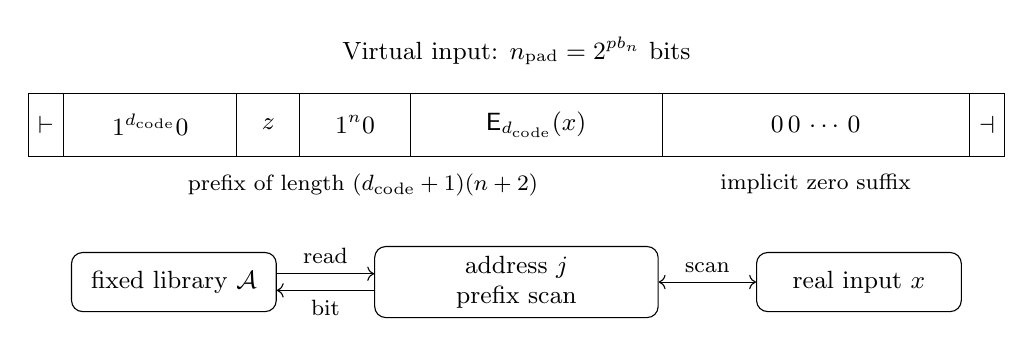
\begin{tikzpicture}[x=1cm,y=1cm,font=\small]
  \draw (0,0) rectangle (12.4,0.8);
  \draw (0.45,0) -- (0.45,0.8);
  \draw (2.65,0) -- (2.65,0.8);
  \draw (3.45,0) -- (3.45,0.8);
  \draw (4.85,0) -- (4.85,0.8);
  \draw (8.05,0) -- (8.05,0.8);
  \draw (11.95,0) -- (11.95,0.8);
  \node at (0.225,0.4) {$\vdash$};
  \node at (1.55,0.4) {$1^{d_{\mathrm{code}}}0$};
  \node at (3.05,0.4) {$z$};
  \node at (4.15,0.4) {$1^n0$};
  \node at (6.45,0.4) {${\mathsf{E}}_{d_{\mathrm{code}}}(x)$};
  \node at (10,0.4) {$0\,0\,\cdots\,0$};
  \node at (12.175,0.4) {$\dashv$};
  \node[anchor=south] at (6.2,1.03)
    {Virtual input: ${n}_{\mathrm{pad}}=2^{{p}{b}_n}$ bits};
  \node[anchor=north,font=\footnotesize] at (4.25,-0.1)
    {prefix of length $(d_{\mathrm{code}}+1)(n+2)$};
  \node[anchor=north,font=\footnotesize] at (10,-0.1)
    {implicit zero suffix};
  \node[draw,rounded corners,align=center,minimum width=2.6cm,
        minimum height=0.75cm] (library) at (1.85,-1.6)
    {fixed library ${\mathcal{A}}$};
  \node[draw,rounded corners,align=center,minimum width=3.6cm,
        minimum height=0.75cm] (callback) at (6.2,-1.6)
    {address ${j}$\\prefix scan};
  \node[draw,rounded corners,align=center,minimum width=2.6cm,
        minimum height=0.75cm] (realinput) at (10.55,-1.6)
    {real input $x$};
  \draw[->] ([yshift=3pt]library.east) -- ([yshift=3pt]callback.west)
    node[midway,above,font=\footnotesize] {read};
  \draw[->] ([yshift=-3pt]callback.west) -- ([yshift=-3pt]library.east)
    node[midway,below,font=\footnotesize] {bit};
  \draw[<->] (callback.east) -- (realinput.west)
    node[midway,above,font=\footnotesize] {scan};
\end{tikzpicture}




 \caption{The fixed library reads the padded input through a callback.
 The callback regenerates prefix symbols from the real input and returns
 zero for an address in the padding interval.}
 \label{fig:compiler-padding}
\end{figure}

\subsection{Read the padded input without storing it}
\label{subsec:compiler-callback}

The padded string can be much longer than the real input. Only its current queried address needs to be stored. A finite routine answers that query by scanning the short encoded prefix and returning zero if the address lies in the padding. We now give the routine explicitly so that its memory is counted alongside the suspended approximator.

Inline the finite transition list of ${\mathcal{A}}$, giving it its own work tapes.
The generated machine ${\mathcal{D}}$ suspends its library control state in finite
control during an input operation.  Four auxiliary binary words suffice:
the length count $n+1$, the virtual right-endmarker address
${n}_{\mathrm{pad}}+1$, the virtual input-head position ${j}$, and a prefix
position ${i}$.  Each has a separate tape, with origin and termination
marks and digits in low-end-first order.

Initialize the length count to one and increment it once per real input
symbol.  Its bit length is exactly
\begin{equation}\label{eq:compiler-bitlength}
 \operatorname{bitlength}(n+1)
   =\lfloor\log_2(n+1)\rfloor+1
   =\lceil\log_2(n+2)\rceil={b}_n
 \qquad(n\ge0).
\end{equation}
For every bit place in that count, write ${p}$ zero bits on the bound tape,
then append a one.  This produces the low-end-first representation of
$2^{{p}{b}_n}={n}_{\mathrm{pad}}$; increment it to obtain
${n}_{\mathrm{pad}}+1$.  The repetition of ${p}$ is hardwired finite control.
Initially set ${j}=0$, the library's left-endmarker position.

At a virtual read, first test ${j}=0$ and ${j}={n}_{\mathrm{pad}}+1$ and return
the corresponding endmarker.  Otherwise initialize ${i}=1$ and regenerate
the prefix in its natural order:
\begin{enumerate}
 \item emit the fixed string $1^{d_{\mathrm{code}}}0z$;
 \item scan $x$, emitting one $1$ per symbol, and then emit $0$;
 \item rewind and scan $x$ again, emitting each fixed-width symbol code
       in ${\mathsf{E}}_{d_{\mathrm{code}}}(x)$.
\end{enumerate}
Here ``emit'' means compare the current ${i}$ with ${j}$, return the bit
if they agree, and otherwise increment ${i}$ and continue.  If the scan
finishes without a match, return zero.  The strings $z$, the integer
$d_{\mathrm{code}}$, symbol codes and emission phases are fixed in
the generated control.  The real input head is rewound by scanning to
its endmarker, without storing its position.  In particular,
${j}={n}_{\mathrm{pad}}+1$ is answered before regeneration, while a padding
address such as ${j}={n}_{\mathrm{pad}}$ returns zero after the finite
prefix scan.  The largest prefix counter value is
${l}_{\mathrm{pre}}+1\le {n}_{\mathrm{pad}}+1$.

For explicit counter routines, an increment uses a finite carry flag.
Compare two low-end-first words by scanning both, retaining only a
finite comparison flag that is overwritten by each higher differing
bit.  After one terminator, treat its later bits as zero using a finite
``ended'' flag.  Rewind each tape to its origin mark afterward.  Zeroing
and copying are likewise bounded bit scans.  No growing arithmetic
register beyond the named words is required.  All words have at most
${p}{b}_n+2$ bits; including delimiters and rewinds, their heads need visit
only positions through ${p}{b}_n+10$.

After the callback, perform the indicated library transition and update
${j}$ in place for its input-head motion.  The library's work heads and
contents are untouched by the callback.  Its state, the returned input
symbol, and any step-local scanned tuple are fixed finite-control data.
The callback does not invoke ${\mathcal{A}}$ recursively or maintain a stack of
callbacks.  The real input head stays between its real endmarkers.

Every listed routine terminates.  For example, a complete regeneration
uses at most ${l}_{\mathrm{pre}}$ emissions, each with an
$O({p}{b}_n+1)$-bit comparison and increment, together with two real-input
scans.  Initialization makes $n$ increments and writes ${p}{b}_n+1$ bound
bits.  These observations give direct polynomial bounds for the
auxiliary operations.  The whole simulation halts because ${\mathcal{A}}$ is total.
Its more uniform explicit time bound, including every such operation,
is derived next from the complete configurations of this same machine.

All the above instructions can be generated as finite transition tables,
unrolling fixed repetitions and strings if necessary.  Formation of the
source list, the integer ${p}$, and this transition table is a finite
effective process.  It makes no test of the source's semantic error or
resource promises.  Syntactically invalid compiler inputs may be assigned
a fixed default output; correctness is required on the stipulated class.
The generated simulation is total and obeys the bounds below even when
the supplied source promises fail; those promises are used to establish
that its decision agrees with the source.

\subsection{Compute explicit bounds for the generated machine}
\label{subsec:compiler-bounds}

All source-dependent choices have now been made by finite operations on code and supplied integers. The remaining bounds use three concrete counts: work tapes, alphabet sizes, and control states. We first bound all live work bits, then count complete configurations of the halting machine, and finally convert finite-alphabet transitions to elementary bit operations.

Use the finite-alphabet description just constructed to compute $t$, its
number of work tapes; $g\ge2$, the maximum of two and its work alphabet
sizes, including all blank, origin and termination symbols; and $q_{\mathcal{D}}$,
its number of states, including callback phases.  Let $u\ge1$ dominate
its explicit transition-table bit length, all alphabet sizes (including
the input alphabet), the number of states, and the number of tapes.
Padding this integer is effective.  Return the positive integer bounds
\begin{equation}\label{eq:compiler-output-bounds}
 \begin{split}
 \rho&=100({p}+2),\qquad
 {s_{\rm bits}}=1+(t+1)(2\rho+1)(g+2),\\
 {k_{\rm space}}&=4{s_{\rm bits}},\qquad c=2{s_{\rm bits}}+1,\qquad
 {h}=2^{(u+100)^2}(q_{\mathcal{D}}+1).
 \end{split}
\end{equation}
These depend on the fixed source and the fixed library, and are computed
from finite syntax.  They have no dependence on $n$ or $x$.

\paragraph{All live work bits.}
Every work head stays in
$[-\rho {b}_n,\rho {b}_n]$.  For a library tape this follows from
Equations~\eqref{eq:compiler-library-box} and
\eqref{eq:compiler-padded-log}, since
$\ell_{\mathrm{pad}}+1={p}{b}_n+2\le\rho {b}_n$.
For an auxiliary tape it follows from
${p}{b}_n+10\le\rho {b}_n$, using ${b}_n\ge1$.
Thus the library's live data and all callback data satisfy the same
bound at the same time.  Encoding a work alphabet of size $g_i$ in
$\max\{1,\lceil\log_2 g_i\rceil\}\le g$ bits per symbol bounds
their total data by
\begin{equation}\label{eq:compiler-space-bound}
 t(2\rho {b}_n+1)g\le {s_{\rm bits}}{b}_n.
\end{equation}
Even twice this quantity satisfies the stronger logarithmic bound: with
${l}_n=\log_2(n+2)\ge1$ we have ${b}_n\le2{l}_n$ and
\[
 2{s_{\rm bits}}{b}_n\le4{s_{\rm bits}}{l}_n={k_{\rm space}} {l}_n.
\]

\paragraph{All finite-alphabet transitions.}
For a fixed real input $x$, a complete configuration is specified by
the state, the real input-head position, all work-head positions, and
all work symbols in the stated intervals.  Everything outside these
intervals remains at its initial value.  There are at most
\begin{equation}\label{eq:compiler-configurations}
 q_{\mathcal{D}}(n+2)(2\rho {b}_n+1)^t
       g^{t(2\rho {b}_n+1)}
 \le q_{\mathcal{D}}(n+2)2^{{s_{\rm bits}}{b}_n}
 \le q_{\mathcal{D}}(n+2)^c
\end{equation}
such configurations.  For the first inequality use
\[
 2\rho {b}_n+1\le(2\rho+1){b}_n,
 \quad \log_2g\le g,
 \quad \log_2(2\rho {b}_n+1)\le(2\rho+1){b}_n;
\]
the second uses ${b}_n\le2\log_2(n+2)$ and $c=2{s_{\rm bits}}+1$.
A deterministic halting computation cannot repeat a complete
configuration.  Therefore Equation~\eqref{eq:compiler-configurations}
bounds its total transitions, including initialization, counter
arithmetic, every regenerated input bit, and every library transition.
The virtual head position is already in the counted word ${j}$; it is
not an additional uncounted configuration component.

\paragraph{Elementary bit operations.}
The preceding count refers to ordinary finite-alphabet transitions.
To charge them in bits, encode each work symbol by a fixed-width block,
mapping blank to the all-zero block.  Read and write within the current
block, return to its first bit, and move to the first bit of the target
block.  Within-block phases and scanned finite tuples are stored in
finite control.  No per-block writable delimiter is needed, and these
operations visit only blocks whose macro positions occur in the proved
work intervals.  Existing origin and termination symbols have already
been included in $g$.  Thus the block implementation obeys the bit-space
estimate above; the factor two also allows the usual blank/bit tape
convention.  Input-symbol access has fixed width and is covered by the
same finite description parameter $u$.

There are at most $u+1$ scanned symbols of at most $u$ bits each.
An explicit sequential comparison against at most $u$ transition rows,
followed by the fixed-width reads, writes and moves, uses at most a
fixed polynomial in $u+1$ bit actions per transition.  For example,
the deliberately loose bound $100(u+1)^8$ suffices for these scans
and comparisons, with all temporary phase and symbol information in
finite control.  It is dominated, for $u\ge1$, by
\[
 100(u+1)^8\le2^{(u+100)^2}.
\]
The binary microcode may have more states than $q_{\mathcal{D}}$, but no new
configuration count is needed: multiply the number of original
transitions by this per-transition bit cost.  Equations~\eqref{eq:compiler-output-bounds}
and~\eqref{eq:compiler-configurations} give the simultaneous bound
\begin{equation}\label{eq:compiler-time-bound}
 \operatorname{time}_{\mathrm{bit}}({\mathcal{D}},x)
 \le {h}(n+2)^c.
\end{equation}
No growing-word arithmetic is charged as a single elementary bit action.

\begin{proof}[Completion of the proof of Theorem~\ref{thm:effective-simulation}]
The compiler returns the described machine ${\mathcal{D}}$ and the integers
${k_{\rm space}},{h},c$ in Equation~\eqref{eq:compiler-output-bounds}.  Its finite
syntactic construction terminates.  On every promised source input,
Equation~\eqref{eq:compiler-exact-probability} and the fixed separator's
threshold guarantee give the correct decision.  The totality of ${\mathcal{A}}$
and the finite callback loops prove halting.  Equations~\eqref{eq:compiler-space-bound}
and~\eqref{eq:compiler-time-bound} give at most ${k_{\rm space}}\log_2(n+2)$
work bits and ${h}(n+2)^c$ bit operations for this same machine.

All claims include $n=0$: then ${b}_n=1$, the real-input scans are empty,
the count $n+1=1$ has one bit, and every displayed padding, strip,
space, and time inequality remains valid.  The library's grouping
width already includes its finitely many small-length exceptions.
All construction constants are fixed before the ordinary input is read.

The work and time internal to probability approximation---environment
enumeration, numerical digits, recursive interfaces, recomputation,
and precision management---belong to the one complete library machine
proved in Theorem~\ref{thm:fixed-precision}.  Its tapes remain counted
throughout virtualization.  The compiler adds only the exact input
operations analyzed here, without an evaluation oracle or an external
stack.  Configuration counting gives polynomial time because this
entire deterministic machine uses exact logarithmic space.
\end{proof}





% ---- sections/related ----
% Pedagogical rewrite, October 8, 2026. Original mathematics: OpenAI.
\section{Historical context and related work}


The complexity of probabilistic Turing machines was developed by
Gill~\cite{Gill1977}, including measures of both time and tape usage.
Random walks made the logarithmic-space question concrete:
Aleliunas, Karp, Lipton, Lov\'asz and Rackoff obtained polynomial-time
randomized algorithms for undirected connectivity and explicitly asked
whether polynomial-time randomized logarithmic space could be simulated
in deterministic logarithmic space~\cite{AleliunasKLLR1979}.
Early work also studied probabilistic machines without a polynomial-time
restriction. Borodin, Cook and Pippenger obtained a quadratic-space
deterministic simulation in this broader setting
\cite{BorodinCookPippenger1983}.
The distinction between a space bound and simultaneous time and space
bounds is essential throughout this history.

Pseudorandom generators attack the problem by replacing a long sequence
of fresh random bits with the output generated from a short seed.
Ajtai, Koml\'os and Szemer\'edi gave early logarithmic-space
constructions that hit small-space tests using short random
strings~\cite{AjtaiKomlosSzemeredi1987}. Babai, Nisan and Szegedy
subsequently obtained pseudorandom generators through multiparty
communication bounds~\cite{BabaiNisanSzegedy1992}.
Nisan's generator uses $O({\mathsf{s}}\log {r})$ seed bits for a space-${\mathsf{s}}$
computation reading ${r}$ random bits~\cite{Nisan1992}.
For logarithmic space and polynomially many bits this gives
$O(\log^2 n)$ seed length; direct seed enumeration has a
quasipolynomial time bound. Nisan's later simultaneous simulation
achieves polynomial time and $O(\log^2 n)$ space
\cite{Nisan1994RLinSC}. Although its title uses $\mathrm{RL}$,
that result includes two-sided bounded error.
For ${\mathsf{s}}(n)\ge\log n$, Nisan and Zuckerman showed that a space-${\mathsf{s}}$
computation using $\operatorname{poly}({\mathsf{s}})$ random bits can be simulated
using only $O({\mathsf{s}})$ random bits and $O({\mathsf{s}})$ space~\cite{NisanZuckerman1996}.
The restriction on the original number of random bits is substantive;
for logarithmic space it permits polylogarithmically many bits.

Saks and Zhou reduced the deterministic space needed for general
bounded-error logarithmic-space computation to
$O(\log^{3/2}n)$~\cite{SaksZhou1999}.
Cai, Chakaravarthy and van Melkebeek established a simultaneous
tradeoff: for each fixed rational $0\le\alpha\le1/2$, the simulation
uses time $n^{O(\log^{1/2-\alpha}n)}$ and space
$O(\log^{3/2+\alpha}n)$
\cite{CaiChakaravarthyVanMelkebeek2006}.
The polynomial-time endpoint has squared-logarithmic space.
Hoza subsequently improved the general space bound to
$O(\log^{3/2}n/\sqrt{\log\log n})$
\cite[Theorem~1.6 and Corollary~A.5]{Hoza2021}.
These smaller space containments do not assert the same polynomial-time
endpoint. Hoza's work also develops weighted pseudorandomness, in which
signed or real weights replace an ordinary probability distribution;
the space-containment improvement and the new weighted-generator
construction are distinct results of that paper.

Acceptance-probability estimation also connects derandomization to
stochastic matrix products and inverses. Ahmadinejad, Kelner, Murtagh,
Peebles, Sidford and Vadhan developed high-precision small-space
algorithms for random-walk probabilities, with stronger bounds for
Eulerian graphs~\cite{AhmadinejadKelnerMurtaghPeeblesSidfordVadhan2020}.
Cohen, Doron, Sberlo and Ta-Shma later used varying precision across
recursion to improve the space complexity of long stochastic matrix
products~\cite{CohenDoronSberloTaShma2023}. The construction in these notes works with a finite inverse on a time-layered configuration graph;
its correction and copy hierarchy controls the information retained
while individual entries are evaluated.

Structural restrictions on a computation provide another route.
For undirected connectivity, Nisan, Szemer\'edi and Wigderson obtained
deterministic space $O(\log^{3/2}n)$~\cite{NisanSzemerediWigderson1992},
subsequently improved to $O(\log^{4/3}n)$ by Armoni, Ta-Shma,
Wigderson and Zhou~\cite{ArmoniTaShmaWigdersonZhou2000}.
Reingold's logarithmic-space algorithm, whose conference version
appeared at STOC 2005, settles undirected connectivity~\cite{Reingold2005,Reingold2008}.
Reingold, Trevisan and Vadhan studied regular directed graphs and gave
logarithmic-space path search for Eulerian directed graphs
\cite{RTV2006}. Their oblivious walk constructions impose additional
labeling conditions. General directed configuration graphs need not
have these properties, so those results did not settle the unrestricted
randomized computation problem.
A read-once branching program is a layered deterministic computation
that reads the input symbols once in a fixed order (bits in the binary
case). Its length is the number of steps,
and its width is the largest number of states in a layer.
A $1/2$-hitting set for a class of programs contains an accepting input
for every member that accepts at least half of all input strings.
The relation between one-sided and two-sided derandomization also
requires care. Cheng and Hoza proved that one uniformly logarithmic-space-enumerable
$1/2$-hitting-set family for all width-$n$, length-$n$ read-once branching
programs would yield
$\mathsf L=\mathsf{BPL}$~\cite{ChengHoza2022}.
The premise is a hitting-set construction; it is not merely the
language-class equality $\mathsf{RL}=\mathsf L$.

Recent results refine both general and structured models.
Chen, Cohen, Doron, Khaskelberg and Ta-Shma improve error reduction for
weighted generators; in the polynomial-width regime their construction
has seed length $\log|\Sigma|+O(\log^2 {\mathsf{t}}+\log(1/\delta))$, where
${\mathsf{t}}$ is branching-program length, $\Sigma$ its alphabet and $\delta$
the error~\cite{ChenCohenDoronKhaskelbergTaShma2026}.
Cheng and Wu obtain simultaneous polynomial-time and polylogarithmic-space
simulations for regular branching programs, with extensions to polynomial-time
randomized logarithmic-space machines whose two-way read-only random tape
visits each cell at most constantly often, and to such machines with read-once randomness
and an auxiliary stack whose push, pop and idle schedule is independent
of the random bits. Consecutive stays on a random-tape cell count as one
visit~\cite[Theorems~5--6]{ChengWu2026SC}.
Hardness-versus-randomness approaches additionally give conditional,
certified and per-instance alternatives; Pyne and Tell survey this
line of work~\cite{PyneTell2026}.

Effectivity has its own substantial antecedents.
Pyne, Raz and Zhan construct a universal deterministic estimator whose
$O({\mathsf{s}}(n))$ space guarantee follows from
$\mathsf{prBPL}\subseteq\mathsf{SPACE}[O({\mathsf{s}}(n))]$, for
space-constructible ${\mathsf{s}}(n)\ge\log n$
\cite[full version, Theorem~5.1]{PyneRazZhan2023}.
Here $\mathsf{prBPL}$ denotes promise problems solvable in polynomial
time and randomized logarithmic space with bounded error.
The compiler in Appendix~\ref{sec:compiler} uses the fixed separator established by the preceding construction
and supplies explicit source-specific numerical resource bounds.
Its construction should be read in this context of universal
simulation, with the source bounds supplied as part of the compiler input.





% ---- sections/notation ----
\section{Notation and a guide to the source symbols}
\label{sec:notation}

The following tables collect the recurring objects. Each is also defined near its first use. Local cutoff constants, finite program tags, and temporary variables are specified in their own sections.

\begin{longtable}{@{}p{.23\textwidth}p{.70\textwidth}@{}}
\toprule
Symbol & Meaning\\ \midrule\endhead
$\mathbf S,\mathbf e$ & Base time-layered transition matrix and final acceptance indicator.\\
$\mathbf p_0$ & Vector of exact continuation probabilities in the base model.\\
$\mathbf C_l,\mathbf w_l$ & Stage-$l$ residual transition matrix and accumulated success vector.\\
$\mathbf E,\mathbf D$ & Cumulative correction and residual $\mathbf C-\mathbf E+\mathbf E\mathbf C$ before copying.\\
$\mathbf G_i,\mathbf G'_i$ & Raw pilot and actual propagation inputs, respectively.\\
$\mathbf g,\mathbf u_i$ & Frozen column multipliers and exact detector scores. The source writes the latter as $U_i$.\\
$\mathbf P_l^r,\mathbf P_l^c$ & One-stage and cumulative weighted projections from copies to their ancestors. The superscript $c$ means cumulative.\\
$\mathbf B_l$ & Cumulative matrix taking the base indicator to $\mathbf w_l$; distinct from a scale-indexed sampling table.\\
$f,\ b_k=2^{-hk}$ & Current entry bound and the fixed geometric grid of nominal retention rates.\\
$a,u,t$ & Entry scale, start-retention rate, and optional usage rate in a sampling task. In numerical sections $t$ is instead a digit clock; the change is stated there.\\
$X_a(y),Y_a(y),Z_a(y)$ & Scalar membership indicators on different sampling channels.\\
$\pi_a$ & Actual retention probability at nominal rate $a$.\\
$\mathbf A,\mathbf F$ & Polynomial coefficient matrix and its frame of nonconstant columns. A local exact correction may instead be denoted $\mathbf E$; the normalized correction table is $\mathbf F$.\\
$p_{\rm fld},l_{\rm box}$ & Prime modulus and retention-box side length.\\
$\mathcal G_h,\mathcal K$ & Integer affine group and a conditional averaging operator.\\
$\mathbf B_b,\mathbf F$ & Normalized sparse bin and correction tables (the source's $\mathcal B_b,\mathcal F$).\\
$m,r$ & Parent accuracy level and child accuracy level. The source uses $M,m$.\\
$p_{\rm acc}$ & Effective statistical accuracy exponent, after scale, domain, and rank charges; the source uses $p$.\\
$i_*,d$ & Dependency rank and a dyadic parent--child level decrease.\\
$b_{\rm mem},n_{\rm v}$ & Size parameter comparable to $\log(n+2)$ and common upper bound on one stage's vertex count; the source uses $B,N$.\\
$l_{\rm max},h,d_0$ & Number of outer stages, fixed dimension/rate exponent, and copy radix; the source uses $L,H,D_0$.\\
$k_{\rm row},j_{\rm det},k_c$ & Fixed row rank, detector rank, and incoming cap; the source uses $K,J,K_c$.\\
$k_*,k_{\rm entry}$ & Fixed sweep count (also a correction row-sum bound), and the residual-entry constant; the source uses $k_*,K_*$.\\
$\mathbf s_i,\mathbf t_i$ & Uncompressed and compressed raw-row prefixes in the compression section.\\
$h_*,\mathcal I_b$ & Fingerprint block width and the $b$th block of accuracy levels.\\
$\mathbf v$ & Shared bit vector used for restoring fingerprint comparisons; the source calls it $V$ in that subsection.\\
$w,w'$ & Parent and child call allowances in the memory accounting, distinct from the success vector $\mathbf w$.\\
$t,j$ & Requested output and operand digit clocks in the arithmetic and controller sections.\\
\bottomrule
\end{longtable}

An overbar marks an estimator when it is compared with its exact target; a pilot correction instead carries a hat. Neither boldface nor case encodes accuracy. In particular, a matrix stays bold uppercase after fixing its random environment. Functions such as the scalar cutoff $\mathsf Q$ and the row functions $\mathsf H$ are named functions, not scalar random variables.

The three independent measures of progress are worth keeping distinct. The outer stage reduces the exact residual. The accuracy level determines which recursive estimator is used. The numerical digit clock asks for a more precise reading of that fixed estimator. Raising the last does not improve the statistical approximation supplied by the second.




% Bibliography embedded to keep this file self-contained.
\begin{thebibliography}{10}

\bibitem{AhmadinejadKelnerMurtaghPeeblesSidfordVadhan2020}
AmirMahdi Ahmadinejad, Jonathan Kelner, Jack Murtagh, John Peebles, Aaron
  Sidford, and Salil Vadhan.
\newblock High-precision estimation of random walks in small space.
\newblock In {\em 61st IEEE Annual Symposium on Foundations of Computer Science
  (FOCS 2020)}, pages 1295--1306. IEEE, 2020.
\newblock Full version: arXiv:1912.04524.

\bibitem{AjtaiKomlosSzemeredi1987}
Mikl{\'o}s Ajtai, J{\'a}nos Koml{\'o}s, and Endre Szemer{\'e}di.
\newblock Deterministic simulation in {LOGSPACE}.
\newblock In {\em Proceedings of the Nineteenth Annual ACM Symposium on Theory
  of Computing}, pages 132--140. Association for Computing Machinery, 1987.

\bibitem{AleliunasKLLR1979}
Romas Aleliunas, Richard~M. Karp, Richard~J. Lipton, L{\'a}szl{\'o} Lov{\'a}sz,
  and Charles Rackoff.
\newblock Random walks, universal traversal sequences, and the complexity of
  maze problems.
\newblock In {\em 20th Annual Symposium on Foundations of Computer Science},
  pages 218--223. IEEE, 1979.

\bibitem{ArmoniTaShmaWigdersonZhou2000}
Roy Armoni, Amnon Ta-Shma, Avi Wigderson, and Shiyu Zhou.
\newblock An {$O(\log(n)^{4/3})$} space algorithm for {$(s,t)$} connectivity in
  undirected graphs.
\newblock {\em Journal of the ACM}, 47(2):294--311, 2000.

\bibitem{Avizienis1963}
Algirdas Avizienis.
\newblock On a flexible implementation of digital computer arithmetic.
\newblock In C.~M. Popplewell, editor, {\em Information Processing 1962}, pages
  664--670. North-Holland, 1963.

\bibitem{BabaiNisanSzegedy1992}
L{\'a}szl{\'o} Babai, Noam Nisan, and M{\'a}ri{\'o} Szegedy.
\newblock Multiparty protocols, pseudorandom generators for logspace, and
  time-space trade-offs.
\newblock {\em Journal of Computer and System Sciences}, 45(2):204--232, 1992.

\bibitem{BenczurKarger2015}
Andr{\'a}s~A. Bencz{\'u}r and David~R. Karger.
\newblock Randomized approximation schemes for cuts and flows in capacitated
  graphs.
\newblock {\em SIAM Journal on Computing}, 44(2):290--319, 2015.

\bibitem{BorodinCookPippenger1983}
Allan Borodin, Stephen Cook, and Nicholas Pippenger.
\newblock Parallel computation for well-endowed rings and space-bounded
  probabilistic machines.
\newblock {\em Information and Control}, 58(1--3):113--136, 1983.

\bibitem{BravermanCohenGarg2020}
Mark Braverman, Gil Cohen, and Sumegha Garg.
\newblock Pseudorandom pseudo-distributions with near-optimal error for
  read-once branching programs.
\newblock {\em SIAM Journal on Computing}, 49(5):STOC18--242--STOC18--299,
  2020.

\bibitem{BuhrmanCleveKouckyLoffSpeelman2014}
Harry Buhrman, Richard Cleve, Michal Kouck{\'y}, Bruno Loff, and Florian
  Speelman.
\newblock Computing with a full memory: Catalytic space.
\newblock In {\em Proceedings of the 46th Annual ACM Symposium on Theory of
  Computing}, pages 857--866. Association for Computing Machinery, 2014.

\bibitem{CaiChakaravarthyVanMelkebeek2006}
Jin-Yi Cai, Venkatesan~T. Chakaravarthy, and Dieter van Melkebeek.
\newblock Time-space tradeoff in derandomizing probabilistic logspace.
\newblock {\em Theory of Computing Systems}, 39(1):189--208, 2006.

\bibitem{CarterWegman1979}
J.~Lawrence Carter and Mark~N. Wegman.
\newblock Universal classes of hash functions.
\newblock {\em Journal of Computer and System Sciences}, 18(2):143--154, 1979.

\bibitem{ChenCohenDoronKhaskelbergTaShma2026}
Ben Chen, Gil Cohen, Dean Doron, Yuval Khaskelberg, and Amnon Ta-Shma.
\newblock Improved error reduction for weighted {PRGs}.
\newblock In {\em Approximation, Randomization, and Combinatorial Optimization.
  Algorithms and Techniques (APPROX/RANDOM 2026)}, volume 392 of {\em Leibniz
  International Proceedings in Informatics}, pages 39:1--39:23. Schloss
  Dagstuhl -- Leibniz-Zentrum f{\"u}r Informatik, 2026.

\bibitem{ChengHoza2022}
Kuan Cheng and William~M. Hoza.
\newblock Hitting sets give two-sided derandomization of small space.
\newblock {\em Theory of Computing}, 18(21):1--32, 2022.

\bibitem{ChengWu2026SC}
Kuan Cheng and Ruiyang Wu.
\newblock {SC} derandomization for regular {ROBPs} and models beyond {BPL},
  2026.
\newblock Version 1, September 20, 2026.

\bibitem{CohenDoronRenardSberloTaShma2021}
Gil Cohen, Dean Doron, Oren Renard, Ori Sberlo, and Amnon Ta-Shma.
\newblock Error reduction for weighted {PRGs} against read once branching
  programs.
\newblock In {\em 36th Computational Complexity Conference (CCC 2021)}, volume
  200 of {\em Leibniz International Proceedings in Informatics}, pages
  22:1--22:17. Schloss Dagstuhl -- Leibniz-Zentrum f{\"u}r Informatik, 2021.

\bibitem{CohenDoronSberloTaShma2023}
Gil Cohen, Dean Doron, Ori Sberlo, and Amnon Ta-Shma.
\newblock Approximating iterated multiplication of stochastic matrices in small
  space.
\newblock In {\em Proceedings of the 55th Annual ACM Symposium on Theory of
  Computing}, pages 35--45. Association for Computing Machinery, 2023.

\bibitem{CookMcKenzie1987}
Stephen~A. Cook and Pierre McKenzie.
\newblock Problems complete for deterministic logarithmic space.
\newblock {\em Journal of Algorithms}, 8(3):385--394, 1987.

\bibitem{Gill1977}
John Gill.
\newblock Computational complexity of probabilistic {Turing} machines.
\newblock {\em SIAM Journal on Computing}, 6(4):675--695, 1977.

\bibitem{Hoza2021}
William~M. Hoza.
\newblock Better pseudodistributions and derandomization for space-bounded
  computation.
\newblock In {\em Approximation, Randomization, and Combinatorial Optimization.
  Algorithms and Techniques (APPROX/RANDOM 2021)}, volume 207 of {\em Leibniz
  International Proceedings in Informatics}, pages 28:1--28:23. Schloss
  Dagstuhl -- Leibniz-Zentrum f{\"u}r Informatik, 2021.

\bibitem{LMT2000}
Klaus-J{\"o}rn Lange, Pierre McKenzie, and Alain Tapp.
\newblock Reversible space equals deterministic space.
\newblock {\em Journal of Computer and System Sciences}, 60(2):354--367, 2000.

\bibitem{MurtaghReingoldSidfordVadhan2017}
Jack Murtagh, Omer Reingold, Aaron Sidford, and Salil Vadhan.
\newblock Derandomization beyond connectivity: Undirected {Laplacian} systems
  in nearly logarithmic space.
\newblock {\em SIAM Journal on Computing}, 50(6):1892--1922, 2021.
\newblock Preliminary version in FOCS 2017.

\bibitem{Nisan1992}
Noam Nisan.
\newblock Pseudorandom generators for space-bounded computation.
\newblock {\em Combinatorica}, 12(4):449--461, 1992.

\bibitem{Nisan1994RLinSC}
Noam Nisan.
\newblock {$\mathrm{RL}\subseteq\mathrm{SC}$}.
\newblock {\em Computational Complexity}, 4(1):1--11, 1994.

\bibitem{NisanSzemerediWigderson1992}
Noam Nisan, Endre Szemer{\'e}di, and Avi Wigderson.
\newblock Undirected connectivity in {$O(\log^{1.5} n)$} space.
\newblock In {\em Proceedings of the 33rd Annual Symposium on Foundations of
  Computer Science}, FOCS '92, pages 24--29. IEEE Computer Society, 1992.

\bibitem{NisanZuckerman1996}
Noam Nisan and David Zuckerman.
\newblock Randomness is linear in space.
\newblock {\em Journal of Computer and System Sciences}, 52(1):43--52, 1996.

\bibitem{PyneRazZhan2023}
Edward Pyne, Ran Raz, and Wei Zhan.
\newblock Certified hardness vs. randomness for log-space.
\newblock In {\em 64th IEEE Annual Symposium on Foundations of Computer Science
  (FOCS 2023)}, pages 989--1007. IEEE, 2023.
\newblock Full version: arXiv:2303.16413.

\bibitem{PyneTell2026}
Edward Pyne and Roei Tell.
\newblock Using hardness vs randomness to design low-space algorithms.
\newblock Electronic Colloquium on Computational Complexity, Report TR26-045,
  2026.

\bibitem{Reingold2005}
Omer Reingold.
\newblock Undirected {ST}-connectivity in log-space.
\newblock In {\em Proceedings of the Thirty-Seventh Annual ACM Symposium on
  Theory of Computing}, STOC '05, pages 376--385. ACM, 2005.

\bibitem{Reingold2008}
Omer Reingold.
\newblock Undirected connectivity in log-space.
\newblock {\em Journal of the ACM}, 55(4):17:1--17:24, 2008.

\bibitem{RTV2006}
Omer Reingold, Luca Trevisan, and Salil Vadhan.
\newblock Pseudorandom walks on regular digraphs and the {RL} vs. {L} problem.
\newblock In {\em Proceedings of the 38th Annual ACM Symposium on Theory of
  Computing}, pages 457--466. Association for Computing Machinery, 2006.

\bibitem{ReingoldVadhanWigderson2002}
Omer Reingold, Salil Vadhan, and Avi Wigderson.
\newblock Entropy waves, the zig-zag graph product, and new constant-degree
  expanders.
\newblock {\em Annals of Mathematics}, 155(1):157--187, 2002.

\bibitem{Riesz1927}
Marcel Riesz.
\newblock Sur les maxima des formes bilin{\'e}aires et sur les fonctionnelles
  lin{\'e}aires.
\newblock {\em Acta Mathematica}, 49:465--497, 1927.

\bibitem{RozenmanVadhan2005}
Eyal Rozenman and Salil Vadhan.
\newblock Derandomized squaring of graphs.
\newblock In {\em Approximation, Randomization and Combinatorial Optimization:
  Algorithms and Techniques}, volume 3624 of {\em Lecture Notes in Computer
  Science}, pages 436--447. Springer, 2005.

\bibitem{SaksZhou1999}
Michael Saks and Shiyu Zhou.
\newblock {$\mathrm{BP}_{\mathrm H}\mathrm{SPACE}(S)\subseteq
  \mathrm{DSPACE}(S^{3/2})$}.
\newblock {\em Journal of Computer and System Sciences}, 58(2):376--403, 1999.

\bibitem{Schwartz1980}
Jacob~T. Schwartz.
\newblock Fast probabilistic algorithms for verification of polynomial
  identities.
\newblock {\em Journal of the ACM}, 27(4):701--717, 1980.

\bibitem{Shalom1999}
Yehuda Shalom.
\newblock Bounded generation and {Kazhdan}'s property {(T)}.
\newblock {\em Publications Math{\'e}matiques de l'IH{\'E}S}, 90:145--168,
  1999.

\bibitem{SpielmanTeng2014}
Daniel~A. Spielman and Shang-Hua Teng.
\newblock Nearly-linear time algorithms for preconditioning and solving
  symmetric, diagonally dominant linear systems.
\newblock {\em SIAM Journal on Matrix Analysis and Applications},
  35(3):835--885, 2014.

\bibitem{Thorin1948}
G.~O. Thorin.
\newblock {\em Convexity theorems generalizing those of {M. Riesz} and
  {Hadamard} with some applications}.
\newblock PhD thesis, Lund University, 1948.
\newblock Russian translation by Yu. T. Medvedev, \emph{Matematika} 1 (1957),
  no.~3, 43--78. \href{https://www.mathnet.ru/eng/mat17}{Translation and
  bibliographic record}.

\end{thebibliography}

\end{document}

